\documentclass[11pt,oneside]{book}
\usepackage{fontspec}
\setmainfont{Noto Serif}
\setsansfont{Noto Sans}
\setmonofont{Noto Sans Mono}
\newfontfamily\proseunicodefont{DejaVu Serif}
\usepackage[margin=1in]{geometry}
\usepackage{microtype}
\usepackage{amsmath,amssymb,amsthm,mathtools,bm}
\usepackage{graphicx}
\usepackage{xcolor}
\usepackage{booktabs}
\usepackage{array}
\usepackage{longtable}
\usepackage{enumitem}
\usepackage{float}
\usepackage{caption}
\usepackage{hyperref}
\usepackage{fancyhdr}
\usepackage{tikz}
\usetikzlibrary{arrows.meta,positioning,calc,decorations.pathmorphing}

\hypersetup{
  colorlinks=true,
  linkcolor=blue!50!black,
  urlcolor=blue!50!black,
  citecolor=blue!50!black
}

\setlength{\parskip}{0.5em}
\setlength{\parindent}{0pt}
\setlist[itemize]{topsep=0.25em,itemsep=0.2em}
\setlist[enumerate]{topsep=0.25em,itemsep=0.2em}
\setlength{\headheight}{40pt}
\numberwithin{equation}{chapter}

\newtheorem{theorem}{نظرية}[chapter]
\newtheorem{proposition}[theorem]{قضية}
\newtheorem{lemma}[theorem]{لمّة}
\newtheorem{corollary}[theorem]{نتيجة}
\theoremstyle{definition}
\newtheorem{definition}[theorem]{تعريف}
\newtheorem{example}[theorem]{مثال}
\theoremstyle{remark}
\newtheorem{remark}[theorem]{ملاحظة}

\providecommand{\ket}[1]{\left\lvert#1\right\rangle}
\providecommand{\bra}[1]{\left\langle#1\right\rvert}
\providecommand{\braket}[2]{\left\langle#1\,\middle|\,#2\right\rangle}
\providecommand{\expect}[1]{\left\langle#1\right\rangle}
\newcommand{\lectureoverview}[1]{\paragraph{نظرة عامة.} #1}

\makeatletter
\newcommand{\course@headerfont}{\normalfont\small\itshape}
\newcommand{\course@pagefont}{\normalfont\small}
\newcommand{\course@headerraise}{14pt}
\newlength{\course@headerboxheight}
\setlength{\course@headerboxheight}{\dimexpr\headheight-\course@headerraise-9pt\relax}
\newcommand{\course@leftheadbox}[1]{%
  \raisebox{\course@headerraise}{%
    \parbox[t][\course@headerboxheight][t]{0.82\textwidth}{%
      \raggedright\course@headerfont\strut\MakeUppercase{#1}\strut%
    }%
  }%
}
\newcommand{\course@rightheadbox}[1]{%
  \raisebox{\course@headerraise}{%
    \parbox[t][\course@headerboxheight][t]{0.82\textwidth}{%
      \raggedleft\course@headerfont\strut\MakeUppercase{#1}\strut%
    }%
  }%
}
\renewcommand{\chaptermark}[1]{\markboth{\MakeUppercase{\chaptername\ \thechapter.\ #1}}{}}
\renewcommand{\sectionmark}[1]{\markright{\MakeUppercase{\thesection\hspace{0.4em}#1}}}
\fancyhf{}
\fancyhead[L]{\course@leftheadbox{\leftmark}}
\fancyhead[R]{\course@pagefont\thepage}
\renewcommand{\headrulewidth}{0.5pt}
\pagestyle{fancy}
\fancypagestyle{plain}{%
  \fancyhf{}
  \fancyhead[L]{\course@leftheadbox{\leftmark}}
  \fancyhead[R]{\course@pagefont\thepage}
  \renewcommand{\headrulewidth}{0.5pt}
}
\makeatother

% Video2Book editorial provenance macros
\newenvironment{classroomqa}{%
  \par\medskip\noindent\begin{minipage}{\linewidth}\small\hrule\medskip
}{%
  \medskip\hrule\end{minipage}\par\medskip
}
\newcommand{\audiencequestion}[1]{\noindent\textbf{سؤال من الحضور.} #1\par\smallskip}
\newcommand{\lecturerresponse}[1]{\noindent\textbf{الإجابة.} #1\par}
\newcommand{\lecturetimestamp}[1]{\footnote{التوقيت في المحاضرة: #1.}}
\newcommand{\lectureframe}[1]{\par\smallskip{\centering\footnotesize\itshape لقطة المحاضرة: #1.\par}}
\newcommand{\editorialnote}[1]{\footnote{توضيح تحريري: #1}}

\usepackage{polyglossia}
\setdefaultlanguage{arabic}
\usepackage{sectsty}
\setotherlanguage{english}
\newfontfamily\arabicfont[Script=Arabic]{Amiri}
\newfontfamily\arabicfontsf[Script=Arabic]{Amiri}
\newfontfamily\arabicfonttt[Script=Arabic]{DejaVu Sans Mono}
\let\arabicsectionnumber\thesection
\let\arabicsubsectionnumber\thesubsection
\renewcommand{\thesection}{\LRE{\arabicsectionnumber}}
\renewcommand{\thesubsection}{\LRE{\arabicsubsectionnumber}}
\renewcommand{\contentsname}{المحتويات}
\renewcommand{\chaptername}{الفصل}
\renewcommand{\figurename}{الشكل}
\renewcommand{\tablename}{الجدول}
\renewcommand{\proofname}{البرهان}
\renewcommand{\bibname}{المراجع}
\sectionfont{\raggedleft}
\subsectionfont{\raggedleft}
\makeatletter
\renewcommand{\@pnumwidth}{2.2em}
\renewcommand{\@tocrmarg}{3.2em}
\makeatother
\usepackage{tocloft}
\renewcommand{\cftchapfont}{\small\bfseries}
\renewcommand{\cftchappagefont}{\small\bfseries}
\renewcommand{\cftsecfont}{\small}
\renewcommand{\cftsecpagefont}{\small}
\setlength{\cftsecnumwidth}{3em}
\renewcommand{\cftsubsecfont}{\small}
\renewcommand{\cftsubsecpagefont}{\small}
\setlength{\cftsubsecindent}{4.5em}
\setlength{\cftsubsecnumwidth}{4em}
\emergencystretch=6em
\pdfstringdefDisableCommands{\def\proseunicodefont{}}

\geometry{paperwidth=177.6mm,paperheight=252mm,left=16mm,right=16mm,
 top=18mm,bottom=18mm,includeheadfoot,headheight=28pt,headsep=7mm,footskip=9mm}
\usepackage{scrextend}
\changefontsizes[17pt]{12pt}
\raggedbottom
\renewenvironment{classroomqa}{\par\medskip\begingroup}{\par\endgroup\medskip}
\fancyhf{}
\setlength{\headwidth}{\textwidth}
\fancyhead[L]{\parbox{\textwidth}{\raggedleft\fontsize{9}{11}\selectfont\nouppercase{\leftmark}}}
\fancyfoot[C]{\small\thepage}
\renewcommand{\headrulewidth}{0.3pt}
\fancypagestyle{plain}{\fancyhf{}\fancyfoot[C]{\small\thepage}\renewcommand{\headrulewidth}{0pt}}

\graphicspath{{../../../generated_course_notes/supplementary/particle_physics_1_basic_concepts/2009_fall/figures/}{../../../generated_course_notes/supplementary/particle_physics_1_basic_concepts/2009_fall/assets/}}
\begin{document}
\frontmatter
\hypersetup{pageanchor=false}
\begin{titlepage}
\hyphenpenalty=10000\exhyphenpenalty=10000
\thispagestyle{empty}
\begin{tikzpicture}[remember picture,overlay]
  \node[anchor=center,inner sep=0] at (current page.center) {%
    \includegraphics[height=\paperheight,keepaspectratio]{../../../generated_course_notes/supplementary/particle_physics_1_basic_concepts/2009_fall/assets/cover-art.png}%
  };
  \node[
    anchor=north west,
    align=right,
    text width=0.78\paperwidth,
    fill=white,
    fill opacity=0.9,
    rounded corners=8pt,
    inner xsep=10pt,
    inner ysep=8pt
  ] at ([xshift=0.08\paperwidth,yshift=-0.06\paperheight]current page.north west) {%
    {\fontsize{30}{33}\selectfont\bfseries\color{black!88} \RLE{فيزياء الجسيمات 1: المفاهيم الأساسية}\\[0.85em]}
    {\large\color{black!72} \RLE{النسخة العربية / خريف 2009}}
  };
  \node[
    anchor=south west,
    align=right,
    text width=0.68\paperwidth,
    fill=white,
    fill opacity=0.82,
    text opacity=1,
    rounded corners=6pt,
    inner sep=12pt
  ] at ([xshift=0.08\paperwidth,yshift=0.08\paperheight]current page.south west) {%
    {\normalsize\color{black!78} \RLE{المحاضرات الأصلية: \LRE{Leonard Susskind}}\\[0.35em]}
    {\small\color{black!72} \RLE{النسخة المصاحبة: \LRE{\href{https://lazying.art}{LazyingArt LLC} / \href{https://github.com/lachlanchen/Video2Book}{Video2Book}}}}
  };
\end{tikzpicture}
\mbox{}
\end{titlepage}
\hypersetup{pageanchor=true}

\clearpage
\chapter*{حول هذه الملاحظات}
تتبع هذه الملاحظات المرافقة، المحررة بصورة مستقلة، محاضرات Leonard Susskind. وقد أُعيد بناؤها من تفريغات آلية، وترجمات مصاحبة، ولقطات مختارة من السبورة، ثم جرى التحقق منها بمقارنتها بالمادة المصدرية المتاحة. وهي ليست مخطوطة أصلية للأستاذ Susskind، ولم يراجعها أو يقرّها.

أُعِدَّت هذه الطبعة بواسطة \href{https://lazying.art}{LazyingArt LLC} باستخدام مسار العمل المفتوح المصدر \href{https://github.com/lachlanchen/Video2Book}{Video2Book}. وتظل التفريغات الآلية متاحةً بصورة منفصلة، وقد تحتوي على أخطاء في التعرّف. ويُشار إلى الإيضاحات التحريرية وعمليات إعادة البناء غير البديهية في الحواشي.
\clearpage
\tableofcontents
\mainmatter
\chapter{الجسيمات والموجات وطاقة الاستبانة}

\section{جسيمات أم حقول؟}

عمَّ تبحث فيزياء الجسيمات؟ الجسيمات---لكن هذه الإجابة تثير فورًا سؤالًا قديمًا. هل الطبيعة متقطعة؟ والمقصود بمتقطعة هنا أن المادة تأتي في وحدات منفصلة غير قابلة للانقسام، لا أنها لبقة. والكلمة اليونانية \emph{أتوم} تعني غير قابل للانقسام، مع أن الأجسام التي تُسمّى اليوم ذرات يمكن تفكيكها. وفي الوقت الراهن، سيكون \emph{جسيم} الاسم العام لوحدة متقطعة.

والتصور المقابل هو المتصل. فالمادة عندئذ ليست مجموعة من القطع المنفصلة، بل توزعًا مستمرًا عبر الفضاء. ولغته الطبيعية هي لغة الحقول. فالحقل دالة في الموضع: كثافة مادة ما حقل، والحقلان الكهربائي والمغناطيسي حقلان أيضًا. وهذان الأخيران يحددان كيف تتحرك الجسيمات المشحونة، لكن الحقول نفسها تُتصوَّر في الوصف الكلاسيكي على أنها موزعة باستمرار في الفضاء.

لا ينبغي التشديد كثيرًا على الترتيب التاريخي لهذه الأفكار. فهذا التسلسل مفيد لأنه يُظهر منطق الحجة، لا لأنه يقدّم تسلسلًا زمنيًا موثوقًا. وتشمل مفردات صورة الجسيمات الذرات والجزيئات والتصادمات والأجسام الموضعية؛ وتشمل مفردات صورة المتصل الحقول والخواص التي تتغير باستمرار. فأيُّ الصورتين صحيحة؟ تمنع ميكانيكا الكم أيًّا منهما من أن تكون صحيحة تمامًا، لكنها تمنع أيضًا أيًّا منهما من أن تكون خاطئة تمامًا.

ستكون المناقشة مكتفية بذاتها جزئيًا، مع أن الحجج اللاحقة تستند إلى ميكانيكا الكم والميكانيكا الكلاسيكية والنسبية الخاصة والكهرومغناطيسية. ومع ذلك يبقى السؤال المباشر أبسط: ما الذي أقنع الناس أولًا بأن المادة متقطعة حقًا؟

\section{الأدلة الكيميائية على أن المادة متقطعة}

جاء أول دليل جاد، على الأقل في هذا العرض المنطقي، من الكيمياء لا من الفيزياء. وهذا التمييز مصطنع: فالكيمياء إلى حد بعيد هي فيزياء الذرات والجزيئات. قارن دالتون كتل أعداد متساوية من جزيئات مواد مختلفة. وكان التحقق من أن العينات تحتوي أعدادًا متساوية من الجزيئات مسألة كبرى بحد ذاتها. وهنا يرد اسم أفوغادرو، والمول هو عدد أفوغادرو من الجزيئات. ولم تكن القيمة الفعلية لذلك العدد لازمة لمجرد مقارنة عينات تحتوي العدد نفسه من الجزيئات.

كان النمط اللافت هو أن الكتل المولية جاءت تقريبًا على هيئة مضاعفات صحيحة للكتلة المولية للهيدروجين. ولم تكن معاملات الضرب عمومًا \(3/2\) أو \(\pi\) أو أعدادًا حقيقية اعتباطية، بل أعدادًا قريبة من الأعداد الصحيحة. فالكربون-12، على سبيل المثال، يحمل تقريبًا اثنتي عشرة من وحدات الكتلة التي يمثلها الهيدروجين. وهذا يوحي بقوة ببناء من لبنات متكررة ذات الكتلة نفسها تقريبًا.

يزيل التفسير الحديث هذا الغموض. فالذرات العادية تحتوي بروتونات ونيوترونات وإلكترونات. ولا تزيد كتلة الإلكترون إلا على نحو جزء واحد من ألفين من كتلة البروتون أو النيوترون، ولذلك تسهم الإلكترونات إسهامًا صغيرًا في الكتلة الذرية. وتحمل البروتونات والنيوترونات تقريبًا كل هذه الكتلة، وتختلف كتلها بأقل بكثير من واحد في المئة. ولأن نواة الهيدروجين العادي بروتون واحد، فإن كتلة الذرة أو الجزيء تكون تقريبًا مضاعفًا صحيحًا لكتلة نووية على مقياس الهيدروجين. وهذا القول تقريبي فحسب: فكتلتا البروتون والنيوترون ليستا متطابقتين، والإلكترونات تسهم بقليل. ومع ذلك يكشف هذا النمط القريب من المضاعفات الصحيحة عن مكوّنات منفصلة.

كان يُنظر إلى الجزيئات آنذاك بوصفها تراكيب من الذرات. وقد حددت كيمياء القرن التاسع عشر نحو مئة نوع من الذرات ونظمتها بوصفها عناصر؛ ويوجد نحو اثنين وتسعين منها طبيعياً في تعداد العناصر، مع تمييزات إضافية حين تُدرج النظائر. وليس الجدول الدوري دورياً بالمعنى الساذج الذي يفترض مجرد تكرار كتل متساوية، لكنه نظّم تلك الأنواع المنفصلة. وفي تلك المرحلة بدت العناصر نفسها كأنها اللبنات الأولية. وقد قدّم عمل أينشتاين 1905 طريقة كمية لترسيخ النظرية الجزيئية للمادة على نحو أكثر حسماً بكثير، لكن الأدلة الكيميائية كانت قد جعلت الصورة الذرية مقنعة بالفعل.

وقبيل نهاية القرن التاسع عشر لم تصمد هذه النهاية الظاهرية. فقد اكتُشف الإلكترون، وكشف النشاط الإشعاعي عن ظواهر لم يستطع التصور الذي يعدّ العناصر أولية أن يستوعبها. وكان النشاط الإشعاعي يتضمن بالفعل، في صورة مصغّرة، كثيراً من الأسئلة التي أصبحت لاحقاً أسئلة الفيزياء النووية وفيزياء الجسيمات.

\section{النشاط الإشعاعي والحزم المفصولة}

الإسناد الدقيق والتسلسل الزمني غير مؤكَّدين. ويُقرن اسم بيكريل، على سبيل التحفّظ، بملاحظة أن مادة مشعة صادف أن كانت بالقرب من صفيحة فوتوغرافية فأثرت فيها كما لو أن إشعاعاً غير مرئي قد أضاءها. وبدلاً من التعامل مع الصفيحة المُضبَّبة بوصفها مجرد صفيحة تالفة، كان يمكن التساؤل عمّا بلغها. وينتمي أيضاً إلى هذا التاريخ عمل ماري كوري الواسع اللاحق، لكن التقسيم الدقيق للاكتشافات المبكرة ليس لازماً للمنطق التجريبي.

ضع المادة عميقاً داخل كتلة كثيفة من الرصاص واترك قناة ضيقة نحو صفيحة فوتوغرافية. والرصاص مفيد لأنه كثيف، في حين تُحزِّم القناة كل ما يفلت. وبدلاً من تعرّض منتشر، تتكوّن على الصفيحة بقعة موضعية، مما يشير إلى حزمة موجَّهة. وبهذا المعنى المنطقي تكون هذه أول حزمة جسيمات، مع أن طبيعتها في هذه المرحلة غير معروفة.

والآن مرِّر الانبعاث المُحزَّم عبر مجال مغناطيسي عمودي على مستوى المسارات. وينفصل الأثر إلى ثلاثة فروع. يستمر أحدها من دون انحراف. وينحني اثنان إلى جهتين متعاكستين، وبمقدارين غير متساويين. وتنعكس جهة القوة المغناطيسية عندما تنعكس إشارة الشحنة، لذا فإن الفرعين المنحنيين على هذا النحو يتصرفان كإشعاعين ذوي شحنتين متعاكستين؛ أما الفرع المستقيم فيتصرف كإشعاع متعادل.\footnote{يعيد هذا الرسم التخطيطي بناء الشكل الذي جرى تطويره في فيديو المحاضرة بين 00:14:34 و00:19:31.}

\begin{figure}[h]
\centering
\begin{tikzpicture}[scale=0.92]
\draw[fill=gray!20] (0,-1.55) rectangle (2.1,1.55);
\draw[fill=white,draw=none] (1.02,-0.13) rectangle (2.12,0.13);
\draw[fill=black] (1.02,0) circle (0.07);
\node[below] at (1.02,-0.12) {\small source};
\node[above] at (1.05,1.55) {\small lead};
\foreach \x in {3.0,3.55,4.1}
  \foreach \y in {-0.55,0,0.55}
    \node at (\x,\y) {\(\otimes\)};
\node[above] at (3.55,0.78) {\small \(\mathbf B\) into the page};
\draw[thick] (7,-1.8) -- (7,1.8);
\node[above] at (7,1.8) {\small plate};
\draw[thick,->] (2.1,0) -- (6.85,0);
\draw[thick,->] (2.1,0) .. controls (4.0,0.05) and (5.35,0.40) .. (6.85,0.88);
\draw[thick,->] (2.1,0) .. controls (3.7,-0.08) and (5.0,-0.75) .. (6.85,-1.42);
\node[right] at (7,0.88) {\small \(\alpha\)};
\node[right] at (7,0) {\small \(\gamma\)};
\node[right] at (7,-1.42) {\small \(\beta\)};
\end{tikzpicture}
\caption{حزمة إشعاعية محزَّمة في مجال مغناطيسي مستعرض. لا ينحرف المركّب المتعادل، بينما تنحني المركّبات ذات الشحنات المتعاكسة إلى جهتين متعاكستين وبمقادير غير متساوية.}
\end{figure}

سُمّيت المكوّنات الثلاثة ألفا وبيتا وغاما. وبالمصطلحات الحديثة،
\begin{equation}
\begin{aligned}
\beta\text{-radiation} &= \text{electrons},\\
\alpha\text{-radiation} &= \text{helium nuclei},\\
\gamma\text{-radiation} &= \text{photons}.
\end{aligned}
\end{equation}
يتألف جسيم ألفا من بروتونين ونيوترونين، وهذا يفسر أن عدده الكتلي أربعة. ومن ثم، في التسلسل التقريبي للأعداد الصحيحة عند دالتون، لكان الهيليوم قد شغل الرقم أربعة: أربع وحدات نووية على مقياس الهيدروجين. أما أشعة بيتا فهي الإلكترونات سالبة الشحنة المعروفة سلفاً من تجارب الأشعة المهبطية. ولا تحمل أشعة غاما أي شحنة كهربائية.

مع مصدر منخفض الكثافة بما يكفي وكاشف قادر على تمييز كل وصول على حدة، يتحول التعريض الذي يبدو مستمرًا إلى تتابع من أحداث منفصلة: نبضة، نبضة، نبضة. ويمكن إجراء الشيء نفسه مع إشعاعات بيتا وألفا وغاما. ويعطي عدّاد غايغر الصورة الصحيحة، سواء أكان أقدم جهاز قد شُغِّل في ذلك النمط التشغيلي تحديدًا أم لا. يصل كل مكوِّن في حزم منفصلة. وتبقى أشعة غاما هي اللغز: فهي عديمة الشحنة، ومع ذلك تُكشَف حدثًا واحدًا في كل مرة. فإشعاع غاما هو ضوء ذو طاقة عالية جدًا، وقد ربط بلانك، وبخاصة أينشتاين، الضوء بالكمّات. لكن قبل مواجهة هذا الاستنتاج، لا بد من أخذ الأدلة الكلاسيكية على أن الضوء موجة على محمل الجد.

\section{الطبيعة الموجية الكلاسيكية للضوء}

في التصور الكلاسيكي، كان الضوء أوضح مثال على الاستمرارية. فهو يتكون من حقول كهربائية ومغناطيسية تنتشر على هيئة موجات متصلة. وكان نيوتن قد فضّل تصورًا جسيميًا، لكن التجارب الموجية أزاحته. إن اهتزاز شحنة يولد إشعاعًا كهرومغناطيسيًا. ويمكن لهوائي عياني أن يصدر موجات راديوية أو موجات ميكروية أو أشعة تحت الحمراء أو ضوءًا مرئيًا أو أشعة فوق بنفسجية؛ والشحنة التي تتحرك داخل الذرة هي أيضًا هوائي. ويمكن للإشعاع المنبعث أن يعرّض لوحًا فوتوغرافيًا.

تعطي فتحة واحدة أول إشارة إلى السلوك الموجي. فلو كان الضوء تيارًا من الرصاصات، لتوقعنا أن تُنتج فتحة صغيرة بقعةً ضيقةً شديدةَ الانحصار. لكن الإضاءة تنتشر بدلًا من ذلك إلى منطقة ضبابية. غير أن الانتشار وحده ليس حاسمًا، إذ يمكن تخيل جسيمات تنحرف بفعل قوى عند حافتها.

وتعطي فتحتان الاختبار الأدق. فسيعطي سيلان جسيميان مستقلان لطختين متداخلتين، ربما تكونان أشد سطوعًا حيث يتداخلان. أما الموجات فتفعل شيئًا مختلفًا. يمكن لقمة من إحدى الفتحتين أن تلتقي قمةً من الأخرى فتتعززا؛ ويمكن أيضًا لقمة أن تلتقي قاعًا فيُلغي أحدهما الآخر. ولذلك تُظهر الشاشة أشرطةً مضيئةً ومظلمةً بالتناوب، بما في ذلك مواضع مظلمة كانت أيٌّ من الفتحتين وحدها ستضيئها.\footnote{يعيد الشكل التخطيطي بناء مخططي الفتحة والتداخل اللذين جرى تطويرهما في فيديو المحاضرة بين 00:25:00 و00:29:49.}

\begin{figure}[h]
\centering
\resizebox{\linewidth}{!}{%
\begin{tikzpicture}[scale=0.88]
\begin{scope}
\draw[->] (-0.3,1.06) -- (0.8,1.06);
\draw[thick] (1.3,0.15) -- (1.3,0.92);
\draw[thick] (1.3,1.20) -- (1.3,2.0);
\draw[thick] (4.8,0.15) -- (4.8,2.0);
\draw[->] (1.34,1.06) .. controls (2.2,1.55) and (3.2,1.55) .. (4.65,1.48);
\draw[->] (1.34,1.06) -- (4.65,1.06);
\draw[->] (1.34,1.06) .. controls (2.2,0.58) and (3.2,0.58) .. (4.65,0.64);
\draw[dashed] (5.45,1.06) ellipse (0.47 and 0.82);
\node at (2.95,2.28) {\small one opening};
\node at (5.45,2.05) {\small broadened spot};
\end{scope}
\begin{scope}[xshift=6.8cm]
\draw[->] (-0.3,1.35) -- (0.8,1.35);
\draw[->] (-0.3,0.75) -- (0.8,0.75);
\draw[thick] (1.3,0.15) -- (1.3,0.62);
\draw[thick] (1.3,0.88) -- (1.3,1.25);
\draw[thick] (1.3,1.51) -- (1.3,2.0);
\draw[thick] (4.8,0.15) -- (4.8,2.0);
\draw[thin] (4.8,0.32) -- (5.18,0.32);
\draw[line width=2pt] (4.8,0.59) -- (5.18,0.59);
\draw[thin] (4.8,0.86) -- (5.18,0.86);
\draw[line width=2pt] (4.8,1.13) -- (5.18,1.13);
\draw[thin] (4.8,1.40) -- (5.18,1.40);
\draw[line width=2pt] (4.8,1.67) -- (5.18,1.67);
\draw[thin] (4.8,1.94) -- (5.18,1.94);
\draw[->] (1.34,0.75) .. controls (2.4,0.82) and (3.5,1.02) .. (4.65,1.13);
\draw[->] (1.34,1.38) .. controls (2.4,1.31) and (3.5,1.20) .. (4.65,1.13);
\draw[->] (1.34,0.75) .. controls (2.4,1.05) and (3.5,1.55) .. (4.65,1.67);
\draw[->] (1.34,1.38) .. controls (2.4,1.55) and (3.5,1.66) .. (4.65,1.67);
\node at (2.95,2.28) {\small two openings};
\node at (5.62,1.13) {\small bright and dark bands};
\end{scope}
\end{tikzpicture}
}
\caption{تُنتِج فتحة واحدة صورةً متسعة، بينما تُنتِج فتحتان تداخلاً بنّاءً وهدّامًا بالتناوب.}
\end{figure}

يسهل تخيّل الأثر نفسه في الماء. حرّك إصبعين على سطحه: تنتشر الموجات الدائرية، وتتَعزَّز في بعض المواضع، وتُلغي بعضها بعضًا في مواضع أخرى. إن التداخل، لا مجرد الانتشار، هو العلامة الحاسمة على السلوك الموجي.

والتسلسل التاريخي، مرة أخرى، ليس بسيطًا. ففي هذا العرض التخطيطي يُقدَّم Huygens قبل Newton بوصفه من أنصار انتشار الموجات؛ ويُربَط Thomas Young ببرهان التداخل؛ كما أن بعض تجارب Newton البصرية نفسها تقبل تفسيرًا قائمًا على تداخل الموجات، رغم أنه كان يفضّل الجسيمات. وقد أثبتت تجارب التداخل اللاحقة الطبيعة الموجية للضوء بما لا يدع مجالًا لشك معقول.

ثم حدّد Maxwell ما الذي يتذبذب. فإذا انتشرت موجة ضوئية على طول محور، فإن مجالها الكهربائي يكون مستعرضًا بالنسبة إلى ذلك المحور. ويكون مجالها المغناطيسي مستعرضًا أيضًا ومتعامدًا على المجال الكهربائي. وينتقل النمط بأكمله بسرعة الضوء.\footnote{يعيد هذا المخطط بناء رسم الموجة الكهرومغناطيسية المرسوم في فيديو المحاضرة عند 00:31:08.}

\begin{figure}[h]
\centering
\begin{tikzpicture}[
  scale=0.9,
  x={(1cm,0cm)},
  y={(0cm,1cm)},
  z={(0.42cm,0.34cm)}
]
\draw[->] (0,0,0) -- (7,0,0) node[right] {\small propagation};
\draw[->] (0,-1.35,0) -- (0,1.35,0) node[above] {\small \(\mathbf E\)};
\draw[->] (0,0,-1.35) -- (0,0,1.35) node[above right] {\small \(\mathbf B\)};
\draw[thick,smooth,variable=\x,domain=0:6.3,samples=100]
  plot ({\x},{sin(\x r)},0);
\draw[thick,dashed,smooth,variable=\x,domain=0:6.3,samples=100]
  plot ({\x},0,{sin(\x r)});
\end{tikzpicture}
\caption{في موجة كهرومغناطيسية، يكون المجالان الكهربائي والمغناطيسي متعامدَين أحدهما على الآخر، وكلاهما مستعرض بالنسبة إلى اتجاه الانتشار.}
\end{figure}

يتذبذب الضوء المرئي العادي بسرعة أكبر بكثير من أن يمكن تتبّع الحقول المتناوبة مباشرةً. وفي موجة راديوية طويلة جدًا، يكون التذبذب أبطأ على نحو مناظر. وفي كلتا الحالتين تؤدي هندسة الموجة المستعرضة نفسها إلى التداخل.

\section{الطول الموجي، والزمن الدوري، والتردد}

الطول الموجي \(\lambda\) هو مسافة مكانية: ابدأ من نقطة في الاهتزاز وتحرك على طول الموجة حتى يتكرر الطور نفسه بعد دورة كاملة. ويُقاس بالأمتار أو بالسنتيمترات أو بأي وحدة طول أخرى.

والآن ابقَ عند موضع واحد بينما تمر الموجة. فالزمن اللازم لدورة كاملة واحدة هو الزمن الدوري \(T\). للضوء المرئي زمن دوري قصير جدًا، تقريبًا من رتبة \(10^{-15}\,\mathrm{s}\)؛ فالطول الموجي الأطول يقابله زمن دوري أطول، والأقصر يقابله زمن دوري أقصر.

خلال زمن دوري واحد، تتقدم الموجة بمقدار طول موجي واحد، لذا فإن موجة سرعتها \(v\) تخضع للعلاقة
\begin{equation}
v=\frac{\lambda}{T}.
\end{equation}
وللموجات المائية والصوتية سرعات انتشارها الخاصة. أما بالنسبة إلى الضوء،
\begin{equation}
c=\frac{\lambda}{T}.
\end{equation}
والتردد \(f\) هو عدد الدورات في وحدة الزمن:
\begin{equation}
f=\frac{1}{T}.
\end{equation}
ومن ثم
\begin{equation}
\lambda f=c.
\end{equation}
ويكفي معرفة الطول الموجي أو التردد لتحديد الآخر.

\begin{figure}[h]
\centering
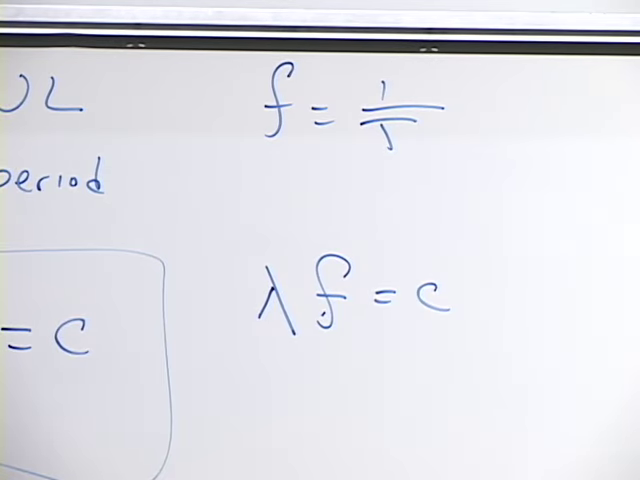
\includegraphics[width=0.68\textwidth]{lecture_01_figure_03.png}
\caption{لموجة ضوئية، \(f=1/T\) و\(\lambda f=c\).}
\lectureframe{00:36:24}
\end{figure}

غالبًا ما يقيس الفيزيائيون معدل الاهتزاز بالراديان في الثانية بدلًا من الدورات الكاملة في الثانية. تخيَّل حركة منتظمة حول دائرة. إذا أكملت النقطة \(f\) دورةً في كل ثانية، وكانت كل دورة تحتوي على \(2\pi\) راديان، فإن ترددها الزاوي هو
\begin{equation}
\omega=2\pi f,
\qquad
\frac{\omega}{2\pi}=f.
\end{equation}
وفي الوقت الحالي هذا مجرد تعريف؛ أما السؤال العملي عما إذا كان يقلل عدد عوامل \(2\pi\) فسيعود لاحقًا.

إن الجمع بين \(f=c/\lambda\) و\(\omega=2\pi f\) يعطي
\begin{equation}
\omega=\frac{2\pi c}{\lambda},
\qquad
\omega\lambda=2\pi c.
\end{equation}
أما لنوع آخر من الموجات، فيُستبدل \(c\) بسرعة انتشار تلك الموجة.

\begin{figure}[h]
\centering
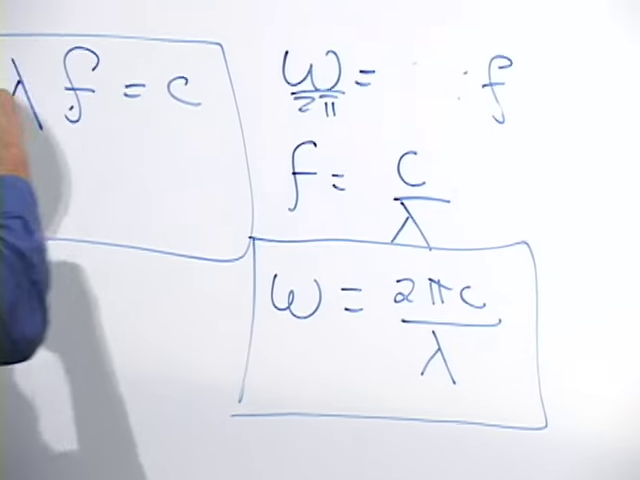
\includegraphics[width=0.68\textwidth]{lecture_01_figure_04.png}
\caption{مع \(\omega=2\pi f\)، تحقق موجة ضوئية \(\omega=2\pi c/\lambda\).}
\lectureframe{00:39:10}
\end{figure}

يشكل الإشعاع الكهرومغناطيسي طيفًا متصلًا. ومرتبةً من الأطول طولًا موجيًا إلى الأقصر، تكون الأسماء المتعارف عليها هي
\begin{equation}
\begin{aligned}
\text{radio}
&\longrightarrow \text{microwave}
\longrightarrow \text{infrared}
\longrightarrow \text{visible}\\
&\longrightarrow \text{ultraviolet}
\longrightarrow \text{X ray}
\longrightarrow \text{gamma ray}.
\end{aligned}
\end{equation}
ولا يشغل الضوء المرئي إلا مجالًا ضيقًا. والحدود بين المناطق المسماة اصطلاحية، لذلك لا حاجة هنا إلى أطوال موجية فاصلة دقيقة. قد تكون الموجات الراديوية طويلة للغاية؛ أما إشعاع غاما فهو الطرف القصير جدًا في الطول الموجي من الطيف الكهرومغناطيسي. وهنا تتضح الصعوبة بحدة: فإشعاع غاما، وفقًا للوصف الكلاسيكي، موجة حقلية متصلة، ومع ذلك يُكتشف على هيئة ومضات منفصلة.

\section{وصولات منفصلة واحتمالات الموجة}

قادت الخواص الثرموديناميكية للإشعاع بلانك وآينشتاين إلى استنتاج أن الضوء يجب أن يُعامل في وحدات منفصلة. وتجربة متخيلة تجعل هذه النقطة جلية، لكنها لا تزعم أنها المسار التاريخي الفعلي إلى الاكتشاف.

سلِّط حزمة على شاشة. عند شدة عادية، تُحدث بقعة مضيئة تبدو متصلة. ضع مُضعِّفًا معتمًا جزئيًا في الحزمة: فتصبح البقعة أخفت. زِد الإضعاف مرارًا فيصل ضوء أقل في وحدة الزمن. وفي النهاية يتغير المظهر. فبدلًا من بقعة خافتة تبدو متصلة، يسجل الكاشف أحداثًا منفصلة.\footnote{يعيد الرسم التخطيطي بناء تجربة الإضعاف كما جرى عرضها في فيديو المحاضرة بين 00:42:32 و00:45:42.}

\begin{figure}[h]
\centering
\begin{tikzpicture}[scale=0.9]
\begin{scope}
\draw[fill=yellow!35] (0,0) circle (0.18);
\draw[->,thick] (0.2,0) -- (2.55,0);
\draw[thick] (2.65,-1.0) -- (2.65,1.0);
\node[below] at (1.4,-1.0) {\small bright beam};
\end{scope}
\begin{scope}[xshift=4.1cm]
\draw[fill=yellow!35] (0,0) circle (0.18);
\draw[->,thick] (0.2,0) -- (1.15,0);
\draw[fill=gray!70] (1.2,-0.85) rectangle (1.55,0.85);
\draw[->,thick] (1.6,0) -- (2.55,0);
\draw[thick] (2.65,-1.0) -- (2.65,1.0);
\node[below] at (1.85,-1.0) {\small strong attenuation};
\end{scope}
\fill[gray!45] (2.62,-0.65) rectangle (2.70,0.65);
\foreach \y in {-0.66,-0.31,0.13,0.58}
  \fill (6.72,\y) circle (0.045);
\node[above] at (2.65,1.0) {\small unresolved exposure};
\node[above] at (6.75,1.0) {\small isolated detections};
\end{tikzpicture}
\caption{يخفض الإضعاف التدريجي معدل الكشف حتى ينحلَّ تعريض يبدو متصلًا إلى أحداث فوتونية منفصلة.}
\end{figure}

إذا انتظرت مدة كافية، تراكمت تلك الأحداث لتكوِّن التوزيع المكاني نفسه للبقعة الأصلية. ولذلك كانت المنطقة المضيئة هي المجموع غير المفصول لوصولات فردية كثيرة. ويمكن إجراء هذا الاختبار عند شدة منخفضة، مع أنه لم يكن التجربة المبكرة التي حفزت في الأصل فرضية الفوتون. وقد نشأ اقتراح آينشتاين للفوتون من اعتبارات ترموديناميكية وكهروضوئية؛ وتوفر تجربة الإضعاف طريقة مباشرة على نحو خاص لتصوُّر نتيجته.

ضع الآن فتحتين في الحزمة وخفِّض الشدة حتى تصل الفوتونات واحدًا تلو الآخر. وكل عملية كشف هي ومضة موضعية. ومع ذلك، بعد عمليات كشف كثيرة، تملأ الومضات نمط تداخل، بما في ذلك أهداب مضيئة ومظلمة. الوصولات المنفصلة عشوائية، لكن توزيع احتمالاتها هو التوزيع الذي يتنبأ به النمط الموجي. لقد أصبحت الموجة الكلاسيكية موجةً تحكم الاحتمالات.

فالموجة والجسيم ليسا إذن نوعين منفصلين من الكيانات يُنسب كل منهما إلى جزء مختلف من الطبيعة. بل هما مظهران لشيء كمومي واحد. ولا يمكن وصف الضوء وصفًا كافيًا على أنه موجة فقط أو جسيم فقط.

أما الإلكترونات فتعكس المفاجأة الأصلية. فقد كان يُسلَّم بأن الإلكترونات جسيمات، وهي تصل إلى كاشف واحدةً تلو الأخرى، لكنها، إذا كانت الفتحات متقاربة بما يكفي، تُنشئ أيضًا نمط تداخل. وجسيمات ألفا، وهي أثقل من الإلكترونات بنحو ثمانية آلاف مرة، تخضع للمبدأ نفسه، وإن كانت التجربة أشد صعوبة. وقد لوحظ التداخل حتى مع buckyballs: جزيئات مكوَّنة من ستين ذرة كربون مرتبة تقريبًا على هيئة كرة قدم معممة. ومن المتوقع أن ينطبق المبدأ نفسه حتى على كرات البولينغ، رغم أن مثل هذه التجربة غير عملية على نحو يكاد يكون خياليًا. ويمكن المضي في المناقشة إلى تجارب مقترحة على الفيروسات أو الخلايا الحية، بوصفها أمثلة يزداد طموحها. وفهم كيف ينسجم الوصفان الموجي والجسيمي يتطلب ميكانيكا الكم؛ أما المهمة المباشرة فهي استخلاص خصائص الفوتون اللازمة لفيزياء الجسيمات.

\section{طاقة الفوتون}

الفوتونات هي العناصر المنفصلة غير القابلة للانقسام للضوء. يحمل الضوء طاقة---فضوء الشمس يسخِّن جسمًا ماصًّا---لذا لا بد أن يحمل كل فوتون طاقة. للموجة الأحادية اللون طول موجي وتردد زاوي محددان، وتكون طاقة كل فوتون فيها:
\begin{equation}
E_\gamma=\hbar\omega.
\end{equation}
ومن المضلل أن نحاول تصور موجة متصلة على أنها تجمّع ميكانيكي صغير من النقاط. وما هو مؤكد هو هذا التركيب التجريبي: تحدث عمليات كشف موضعية وفق توزيع تحكمه الموجة، وتصل الطاقة في وحدات غير قابلة للانقسام.

وبما أن
\begin{equation}
\omega=\frac{2\pi c}{\lambda},
\end{equation}
فإن الطول الموجي الأقصر يعني ترددًا زاويًا أكبر، ومن ثم طاقة أكبر في كل فوتون:
\begin{equation}
\lambda\downarrow
\quad\Longrightarrow\quad
\omega\uparrow
\quad\Longrightarrow\quad
E_\gamma\uparrow.
\end{equation}
طاقة الفوتون الراديوي الواحد صغيرة جدًا. ومع ذلك، يمكن لحزمة راديوية أن تحمل طاقة كلية هائلة لأنها تحتوي على عدد كبير جدًا من الفوتونات. ولنبضة أحادية اللون تحتوي على \(n\) فوتونًا،
\begin{equation}
E_{\text{pulse}}=n\hbar\omega,
\qquad
n=0,1,2,\ldots.
\end{equation}
قد يكون المجموع كبيرًا، لكنه يظل مضاعفًا صحيحًا لطاقة الفوتون الواحد.

تشير هذه العلاقة إلى السؤال العملي الذي سيحكم بقية المناقشة. لماذا يجب بناء آلات أكبر فأكبر لرؤية أشياء أصغر فأصغر؟ ولماذا لا نستخدم آلة صغيرة لشيء صغير؟ النصف الأول من الجواب حاضر بالفعل: فتمييز بنية أصغر فأصغر يتطلب طولًا موجيًا أقصر، والكم ذو الطول الموجي الأقصر يحمل طاقة أكبر.

\section{طاقة السكون والكتلة اللامتغيرة}

تجمع فيزياء الجسيمات بين ميكانيكا الكم والنسبية. وتوفّر علاقة الفوتون \(E_\gamma=\hbar\omega\) الجانب الكمّي؛ أمّا الحقيقة الأولية المناظرة من النسبية فهي
\begin{equation}
E_{\mathrm{rest}}=mc^2.
\end{equation}
وهذا التقييد مهم. فقد ميّزت العروض الأقدم بين \emph{كتلة السكون} وبين \emph{الكتلة المتحركة} المعتمدة على السرعة. ويستعمل الاصطلاح الحديث \emph{الكتلة} للدلالة على الكتلة الثابتة لجسم ما. فالحركة تغيّر طاقته لا كتلته. ولكل إلكترون الكتلة نفسها مهما كانت حالته الحركية، في حين تزداد طاقة الإلكترون كلما عُجِّل. ومن ثم فإن \(E=mc^2\)، في هذه الصيغة، هي طاقة جسم ذي كتلة في إطار يكون فيه الجسم ككل ساكنًا.

ليس من الضروري أن يكون الجسم ساكنًا داخليًا. يمكن لصندوق من الغاز أن يبقى ساكنًا على ميزان بينما تتحرك جزيئاته بسرعة في جميع الاتجاهات. وطاقة تلك الحركات الداخلية جزء من طاقة السكون للصندوق بأكمله. ابدأ بصندوق بارد، وقِس كتلته، ثم أضف طاقة حرارية مع إبقاء الصندوق نفسه ساكنًا. فتتغير كتلته الساكنة بمقدار
\begin{equation}
\Delta m=\frac{\Delta E_{\mathrm{internal}}}{c^2}.
\end{equation}
ويزداد وزنه وقصوره الذاتي مع كتلته. وبالنسبة إلى صندوق عادي، حتى بعد ارتفاع كبير في درجة الحرارة، يكون الأثر أصغر بكثير من أن يُلاحظ على ميزان عادي؛ وصِغَر الأثر لا يغيّر المبدأ.

ويأتي مثال أوضح باستخدام إلكترون وبوزيترون. فلهما كتلتان متساويتان تمامًا وشحنتان كهربائيتان متعاكستان. وإذا كانا في البداية ساكنين ثم أفنيا بعضهما، حملت الفوتونات الطاقة بعيدًا:
\begin{equation}
e^-+e^+\longrightarrow \text{photons}.
\end{equation}
والطاقة الابتدائية هي
\begin{equation}
E_{\mathrm{initial}}=2m_e c^2,
\end{equation}
ولا يمكن لتلك الطاقة أن تختفي. ولا يعطي زوج واحد إلا مقدارًا ضئيلًا جدًا، لذا يلزم عدد هائل من الأزواج لتسخين حتى فنجان من القهوة، لكن أحداث الإفناء الفردية تُظهر التحول مباشرةً.

لذلك، بالنسبة إلى جسم ساكن، تكون الكتلة والطاقة الكمية الفيزيائية نفسها مُعبَّرًا عنها بوحدتين مختلفتين. والعامل \(c^2\) هو عامل التحويل بين وحدات الكتلة والطاقة المألوفة، تمامًا كما يحوّل عامل عددي الأمتار إلى سنتيمترات.

\begin{classroomqa}
\lecturetimestamp{01:04:39}
\audiencequestion{هل يتطلب تحويل الكتلة إلى طاقة منطلقة آليةً ما؟}
\lecturerresponse{نعم، يلزم وجود آلية فيزيائية، لكن قوانين الانحفاظ تقيّد نتيجتها سلفًا. فحتى قبل وصف آلية الإفناء المجهرية، لا بد أن تعاود الظهور في مكان ما الطاقة الابتدائية للإلكترون--البوزيترون. لذلك يمكن لانحفاظ الطاقة أن يحدد جزءًا مهمًا من الجواب من غير عرض تفصيلي للتفاعل.}
\end{classroomqa}

\section{الأبعاد واختيار الوحدات}

في وحدات النظام الدولي، تكون سرعة الضوء عددًا كبيرًا جدًا ويكون ثابت بلانك عددًا صغيرًا جدًا. ويُوحي بصِغَر هذا الأخير أصلًا علاقة الفوتون: فالتردد الزاوي للضوء المرئي هائل، في حين أن طاقة فوتون واحد ضئيلة، لذا تتطلب \(E_\gamma=\hbar\omega\) قيمة عددية صغيرة لـ\(\hbar\) في هذه الوحدات. وعلى مستوى رتبة المقدار،
\begin{equation}
c\sim 10^8\ \mathrm{m\,s^{-1}},
\qquad
\hbar\sim 10^{-34}\ \mathrm{J\,s}.
\end{equation}
\editorialnote{لم يُحتفَظ إلا برتب المقدار المذكورة في المحاضرة لأن الأرقام الأخيرة على اللوح غير واضحة.}
والوحدات أساسية: فليس أيٌّ من الثابتين مجرد عدد عشري صرف. وبما أن للطاقة الأبعاد
\begin{equation}
[E]=M L^2 T^{-2},
\end{equation}
وأن \(E_\gamma=\hbar\omega\) مع \([\omega]=T^{-1}\)، فإن ثابت بلانك له الأبعاد
\begin{equation}
[\hbar]=[E]T=M L^2 T^{-1}.
\end{equation}

إن وصف \(c\) بالكِبَر و\(\hbar\) بالصِّغَر يفترض سلفًا اختيارًا للوحدات. فقياس السرعة بالأقدام في الساعة يعطي قيمة عددية لـ\(c\) تختلف عن قياسها بالأمتار في الثانية. وبوحدات السنوات الضوئية لكل سنة، أو الثواني الضوئية لكل ثانية، تكون سرعة الضوء ببساطة واحدًا. وبالمثل، يمكن لاختيار مناسب ومنسق لوحدات الكتلة والطول والزمن أن يجعل \(\hbar=1\).

أنظمة الوحدات المألوفة أعراف متوارثة، لا خصائص مميزة للطبيعة. فالميل الواحد يضم 5280 قدمًا، ووحدة stone تضم أربعة عشر رطلًا، وتُقاس الخيول بوحدة اليد، وقد تُقاس القدرة بالقدرة الحصانية. والوحدات المترية أكثر انتظامًا، لكن مقاييسها تظل اختيارات بشرية. وليس في الفيزياء الأساسية ما يميّز المتر أو الثانية أو الكيلوغرام.

يتيح الطول والزمن والكتلة ثلاثة اختيارات أساسية مستقلة للوحدات:
\begin{equation}
L,\qquad T,\qquad M.
\end{equation}
ويمكن بناء سائر الوحدات الميكانيكية منها. وتعتمد الاختيارات المفيدة على المسألة. فكتلة شمسية مريحة في الفيزياء الفلكية؛ وقد تكون كتلة البروتون مريحة في الفيزياء النووية؛ كما تجعل السنوات الضوئية والسنوات الصيغ الفلكية النسبية أكثر إيجازًا. ومع وجود ثلاثة اختيارات مستقلة، يمكن إسناد قيم عددية مناسبة إلى ثلاثة ثوابت ذات أبعاد مستقلة. وليس من الضروري أن تتخذ الفيزياء الفلكية والفيزياء الذرية وفيزياء الجسيمات الاختيارات نفسها.

في فيزياء الجسيمات، هناك اصطلاحان مفيدان على نحو خاص هما
\begin{equation}
c=1,
\qquad
\hbar=1.
\end{equation}
ولا توجد كتلة لجسيم تتميز على نحو مماثل بالنسبة إلى الوحدة المتبقية. ويمكن للمرء أن يعلن أن كتلة البروتون، أو كتلة بوزون هيغز، أو كتلة الميون تساوي واحدًا، لكن ذلك لن يكون إلا تفضيلًا لعنصر واحد من مجموعة كبيرة.

فلماذا نختار \(c\) و\(\hbar\) إذن؟ قد يكون الجواب الأول أنهما يظهران في معادلات كثيرة. لكن كثرة الظهور لا تكفي: فكتلة البروتون تظهر أيضًا في معادلات كثيرة، وكذلك حجم البروتون. وما يميز \(c\) و\(\hbar\) هو كونيتهما.

الثابتان \(c\) و\(\hbar\) مختلفان. فالسرعة \(c\) تقيّد كل جسم فيزيائي: إذ يمكن للأجسام ذات الكتلة أن تقترب منها، ولكن لا يمكن تسريعها لتتجاوزها. ويقيّد ثابت بلانك كل جسم كمومي من خلال علاقة الارتياب على مستوى رتبة المقدار
\begin{equation}
\Delta x\,\Delta p\gtrsim\hbar.
\end{equation}
ولا تخص أيٌّ من العبارتين نوعًا بعينه من الجسيمات. وهذه الكونية هي ما يجعل \(c=1\) و\(\hbar=1\) اصطلاحين طبيعيين.

ولا يوفّر البروتون مقياسًا كونيًا مماثلًا. فهو مجرد جسم واحد بين أشياء كثيرة. وجعل كتلة البروتون مساوية لواحد لا يتمتع بمكانة أكثر أساسية من جعل كتلة ذرة روبيديوم مساوية لواحد؛ ويعرض الإلكترون وبوزون هيغز والميون الصعوبة نفسها.

وتوحي الشحنة الكهربائية بكمية كونية أخرى، لكن بعد جعل \(c\) و\(\hbar\) مساويين لواحد، يصبح الاقتران الكهرومغناطيسي ذو الدلالة الفيزيائية بلا أبعاد. ويمكن لتغيير الوحدات أن ينقل الثوابت ذات الأبعاد داخل صيغة كهرومغناطيسية؛ لكنه لا يستطيع تغيير اقتران حقيقي بلا أبعاد.

وتوفّر الجاذبية ثابتًا كونيًا ذا أبعاد. ففي الصيغة النيوتونية، يكون مقدار القوة بين كتلتين
\begin{equation}
F=G\frac{m_1m_2}{r^2}.
\end{equation}
وكل كتلة تتفاعل ثقاليًا، في حين إن الأجسام المتعادلة كهربائيًا ليست مضطرة إلى المشاركة في قوة كهربائية. ومن ثم يملك \(G\) الكونية المطلوبة. ومع ذلك، فهو تطبيع عملي رديء لفيزياء الجسيمات العادية، لأن قوى الجاذبية بين الجسيمات الأولية المعروفة مهملة في الحسابات موضع النقاش.

\begin{classroomqa}
\lecturetimestamp{01:20:34}
\audiencequestion{هل يصح ببساطة استبعاد \(G\)؟ فعند طاقات عالية جدًا قد لا تطيع الجسيمات الأولية الجاذبية الكلاسيكية على النحو المفترض.}
\lecturerresponse{تستجيب الجسيمات المفردة فعلًا لحقل الجاذبية الأرضي: فالجسيم الواحد يسقط في ذلك الحقل. ولم يُقَس الأثر الثقالي لجسيم أولي واحد على آخر قياسًا مباشرًا، لذا يمكن التشكيك في افتراض الكونية عند ذلك المستوى. والسبب المباشر لترك \(G\) خارجًا هو سبب عملي لا مطلق: فالجاذبية تسهم إسهامًا مهملًا في تجارب فيزياء الجسيمات العادية ومعادلاتها.}
\end{classroomqa}

\begin{classroomqa}
\lecturetimestamp{01:22:01}
\audiencequestion{هل يمكن استعمال التفاعل الكهربائي بوصفه الاصطلاح الثالث لتحديد الوحدات بدلًا من الجاذبية؟}
\lecturerresponse{نعم. يمكن اختيار وحدات كهرومغناطيسية تُطبَّع فيها الشحنة الكهربائية، أو الثابت الذي يظهر في قانون كولوم. وتُستعمل مثل هذه الاصطلاحات. فالإلكترونات تتنافر بدلًا من أن تتجاذب، لكن تلك الإشارة لا تعوق الاختيار. إنه ببساطة ليس الاصطلاح المعتمد هنا.}
\end{classroomqa}

\begin{classroomqa}
\lecturetimestamp{01:23:06}
\audiencequestion{بمجرد جعل \(c\) و\(\hbar\) مساويين لواحد، هل تصبح الشحنة الكهربائية بلا أبعاد؟}
\lecturerresponse{نعم. فهناك مقدار بلا أبعاد يرتبط بمربع الشحنة الكهربائية يساوي تقريبًا \(1/137\). ويمكن إرجاء الاصطلاح الدقيق ومعنى ذلك العدد؛ والنقطة هنا هي أنه بلا أبعاد.}
\end{classroomqa}

\begin{classroomqa}
\lecturetimestamp{01:23:37}
\audiencequestion{هل يمكن اختيار ثابت كولوم بوصفه الثابت الثالث الذي يُجعل مساويًا لواحد؟}
\lecturerresponse{يمكن امتصاصه في اصطلاح الوحدات الكهرومغناطيسية. ولا يمكن لهذا الاختيار أن يحوّل الاقتران اللابُعدي \(1/137\) إلى واحد، لأن تغيير الوحدات لا يمكن أن يغيّر عددًا بلا أبعاد. ولا يُدَّعى هنا أي نفع خاص من اعتماد ذلك الاصطلاح.}
\end{classroomqa}

\section{معادلات الوحدات الطبيعية والأطر المرجعية}

مع \(c=1\)، تصبح علاقة طاقة السكون لجسم ذي كتلة على الصورة
\begin{equation}
E_{\mathrm{rest}}=m.
\end{equation}
ومع \(\hbar=1\)، تصبح علاقة الفوتون على الصورة
\begin{equation}
E_\gamma=\omega.
\end{equation}
ويمكن إعادة إدخال الثابتين كلما احتيج إلى مقادير عددية بوحدات مألوفة.

\begin{figure}[h]
\centering
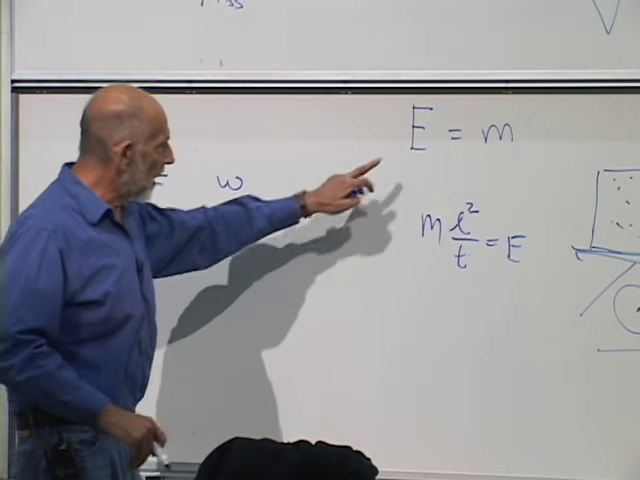
\includegraphics[width=0.72\textwidth]{lecture_01_figure_05.png}
\caption{في وحدات يكون فيها \(c=1\)، تكون طاقة السكون لجسم ذي كتلة في حالة سكون هي \(E=m\).}
\lectureframe{01:25:40}
\end{figure}

تبدو هذه الصيغ متشابهة، لكنها تعني أشياء مختلفة. في \(E_{\mathrm{rest}}=m\)، تمثل \(E\) طاقة السكون لجسم ذي كتلة. والفوتون عديم الكتلة ولا يمكن إحضاره إلى السكون، لذا فإن طاقته ليست طاقة سكون. وتعطي العلاقة \(E_\gamma=\omega\) طاقة كمٍّ متحرك عديم الكتلة.

\begin{classroomqa}
\lecturetimestamp{01:26:07}
\audiencequestion{ما معنى \emph{في حالة سكون} عندما يكون السكون دائمًا بالنسبة إلى شيء ما، والمختبر نفسه ليس في سكون مطلق؟}
\lecturerresponse{يُعرَّف السكون بالنسبة إلى إطار مختار. فإذا كان كوب ساكنًا بالنسبة إلى المختبر، فإن طاقته في إطار المختبر ذاك هي كتلته عندما \(c=1\)، من دون أي إسهام حركي كلي. أما راصد آخر يمر بجانب الكوب فيسند إليه طاقة حركية أيضًا. وبوجه عام، يسند راصدون مختلفون طاقات مختلفة إلى الجسم نفسه أو إلى الفوتون نفسه؛ فالطاقة تعتمد على الإطار المرجعي، ولا يقتضي ذلك أي ادعاء بوجود سكون مطلق.}
\end{classroomqa}

يمكن الآن إعادة النظر في اصطلاح التردد الزاوي. إن كتابة \(E_\gamma=\hbar\omega\) موجزة، لكن \(\omega=2\pi f\) أدخلت عاملًا مقداره \(2\pi\) في وقت سابق.

\begin{classroomqa}
\lecturetimestamp{01:28:13}
\audiencequestion{لماذا نستخدم التردد الزاوي \(\omega\)، المقاس بالراديان في الثانية، بدلًا من العدد الذي يبدو أبسط للدورات الكاملة في الثانية؟}
\lecturerresponse{الاختيار تاريخي جزئيًا، والإجابة الرياضية عملية أكثر منها مباشرة. والإجابة المطروحة هنا مبدئية: اكتب المعادلات ذات الصلة مرة باستعمال \(f\) ومرة باستعمال \(\omega\)، ثم انظر أي الاصطلاحين يترك عوامل أقل من \(2\pi\). ولا يمكن جعل عوامل \(2\pi\) تختفي في كل موضع. وقد اقتُرح أيضًا ارتباط محتمل بترميز الأسّ المركب، لكنه لا يُطوَّر هنا.}
\end{classroomqa}

\begin{classroomqa}
\lecturetimestamp{01:29:51}
\audiencequestion{هل يمكن تسريع جسيمين حتى يصبح تفاعلهما الثقالي المتبادل مهمًّا؟}
\lecturerresponse{من حيث المبدأ، نعم. أما عمليًا، فالمعجلات الحالية بعيدة على نحو استثنائي عن ذلك النطاق. وتعتمد الإجابة أيضًا على المقصود بكلمة جسيم: فالجسم العياني ذو الجاذبية ليس هو حالة الجسيم الأولي المقصودة هنا.}
\end{classroomqa}

\begin{classroomqa}
\lecturetimestamp{01:30:27}
\audiencequestion{ما الذي يمكن أن يكون مصدرًا للبوزيترونات؟}
\lecturerresponse{يمكن للتصادمات عالية الطاقة أن تُنتج بوزيترونات. كما تنتجها بعض العمليات النووية وبعض الاضمحلالات أيضًا.}
\end{classroomqa}

\begin{classroomqa}
\lecturetimestamp{01:30:53}
\audiencequestion{هل زمن بلانك ومسافة بلانك هما الوحدتان الطبيعيتان المستخدمتان هنا؟}
\lecturerresponse{لا. تنشأ وحدات بلانك عندما تُجعل \(G\) و\(c\) و\(\hbar\) جميعها مساويةً للواحد. ويكون طول بلانك الناتج أصغر بكثير من مقاييس الطول المعتادة في فيزياء الجسيمات، لذا فهو مقياس غير ملائم هنا. وتكون مثل هذه الوحدات طبيعية عندما تكون الجاذبية وميكانيكا الكم والنسبية كلها مهمة معًا، كما في فيزياء الثقوب السوداء أو علم الكونيات أو الجاذبية الكمومية. وعندما تكون الجاذبية مهملة، يكون جعل \(c\) و\(\hbar\) فقط مساويين للواحد أكثر فائدة.}
\end{classroomqa}

\section{الزخم والضوء والاستبانة}

المفهوم الأساسي التالي هو الزخم. الجسم الساكن لا يملك زخمًا، مع أن له طاقة سكون غير منعدمة هي \(mc^2\). وما إن يتحرك حتى يحمل، في العموم، زخمًا. ويُحفَظ الزخم في التصادم كما تُحفَظ الطاقة: فعندما يتصادم جسمان، يكون الزخم المتجهي الكلي قبل التصادم وبعده هو نفسه. وأي شيء يقيّده قانون حفظ يستحق اهتمامًا خاصًا.

الزخم كمية متجهة: فهو يشير في اتجاه الحركة. ولجسم غير نسبي،
\begin{equation}
\mathbf p=m\mathbf v.
\end{equation}
وليست هذه هي الصيغة النسبية العامة، ولا يمكن تطبيقها مباشرة على الضوء.

ومع ذلك، يحمل الضوء زخمًا كما يحمل طاقة. ويولد الضوء العادي دفعًا ضئيلًا جدًا بحيث يصعب ملاحظة زخمه، لكن نبضة ليزر شديدة يمكن أن تنقل اندفاعًا معتبرًا. فالليزر الكبير في Livermore، على سبيل المثال، يمكنه أن يدفع المادة إلى الداخل بالزخم الذي يحمله إشعاعه.

تأمل نبضة ذات توازٍ جيد بما يكفي بحيث تسير أشعتها تقريبًا على طول محور واحد. وقد يكون للحزمة الحقيقية بعض الانتشار الزاوي، بحيث تسير أجزاء منها في اتجاهات مختلفة قليلًا، لكن في الحزمة المثالية المتوازية يشير الزخم على امتداد الحزمة ويكون مقداره
\begin{equation}
p=\frac{E}{c},
\qquad\text{or equivalently}\qquad
E=cp.
\end{equation}
وتُتخذ هذه العلاقة هنا بوصفها حقيقة نسبية بدلًا من البرهنة عليها. ولا يؤكد الفحص البعدي الآتي إلا أن وحداتها تتفق مع وحدات الزخم المعتاد:
\begin{equation}
\left[\frac{E}{c}\right]
=
\frac{M L^2 T^{-2}}{L T^{-1}}
=
M L T^{-1}
=
[m v]
=
[p].
\end{equation}
ولا تُسنِد هذه المقارنة البعدية كتلة سكون إلى الضوء. فالفوتون كتلته صفر؛ وهو يحمل زخمًا لأنه يحمل طاقة ويتحرك بسرعة \(c\).

اتجاه \(\mathbf p\) هو اتجاه الانتشار. وعادةً يصعب كشف مقداره لأن \(c\) تظهر في المقام. ويمكن للحزمة أن تكشف عن طاقتها بسهولة بتسخين المادة أو تبخيرها، في حين يكون دفعها الميكانيكي أصغر بكثير. ومع شدة كافية، يمكن أن يصبح ذلك الدفع كبيرًا.

لفوتون واحد،
\begin{align}
p_\gamma
&=\frac{E_\gamma}{c}\\
&=\frac{\hbar\omega}{c}.
\end{align}
وللتعبير عن ذلك بدلالة الطول الموجي، نعود بحذر إلى علاقات الموجة. وبما أن
\begin{equation}
f\lambda=c,
\qquad
\omega=2\pi f,
\end{equation}
فالعلاقة الصحيحة هي
\begin{equation}
\omega\lambda=2\pi c,
\qquad
\omega=\frac{2\pi c}{\lambda}.
\end{equation}
ومن السهل قلب عامل \(2\pi\) إذا لم تُكتب التعريفات صراحةً. والبدء من جديد من \(f\lambda=c\) و\(f=\omega/(2\pi)\) يحسم الأمر:
\begin{equation}
\frac{\omega}{2\pi}\lambda=c
\quad\Longrightarrow\quad
\omega\lambda=2\pi c.
\end{equation}
ويعطي التعويض الآن
\begin{align}
p_\gamma
&=\frac{\hbar}{c}\frac{2\pi c}{\lambda}\\
&=\frac{2\pi\hbar}{\lambda}\\
&=\frac{h}{\lambda}.
\end{align}

\begin{classroomqa}
\lecturetimestamp{01:42:38}
\audiencequestion{هل \(2\pi\hbar\) يساوي \(h\)؟}
\lecturerresponse{نعم. فبحسب التعريف \(h=2\pi\hbar\)، لذا فإن \(p_\gamma=2\pi\hbar/\lambda\) هو نفسه \(p_\gamma=h/\lambda\). وتظهر عوامل \(2\pi\) من جديد في موضع ما أيًّا كان اصطلاح التردد المختار.}
\end{classroomqa}

كلما قصر الطول الموجي كبر زخم الفوتون. لفوتون الراديو طول موجي طويل جدًا وزخم ضئيل جدًا. أما فوتون أشعة غاما فطوله الموجي قصير جدًا ودفعتُه أكبر بكثير. ولا يزال فوتون واحد لا يعطي إلا اندفاعًا عيانيًا صغيرًا، لكن زخمه أكبر بكثير من زخم فوتون راديو. وطاقته أكبر أيضًا، لأن \(E_\gamma=cp_\gamma\).

تفسر هذه العلاقة لماذا تتطلب الأجسام الأصغر آلات أكبر. فالصورة الملتقطة بأطوال موجية أطول بكثير من رأس الإنسان لا يمكن أن تُظهر إلا غشاوة. ولتمييز ملامح الوجه، يجب أن يكون الطول الموجي أقصر من الرأس. ولتمييز شعرة واحدة، يجب أن يكون مماثلًا لسماكة الشعرة أو أصغر منها. ولتمييز بنية ذرة، يجب ألا يزيد الطول الموجي للمسبار على الذرة:
\begin{equation}
\lambda_{\mathrm{probe}}\lesssim
\text{size of the structure to be resolved}.
\end{equation}
ولذلك تتطلب البنى الأصغر أطوالًا موجية أقصر، وتتطلب الأطوال الموجية الأقصر زخمًا وطاقة أكبر. ولا يلزم أن يكون المسبار فوتونًا؛ فالجسيمات العالية الطاقة من أنواع أخرى تخضع للصلة الكمومية نفسها بين الطول الموجي والزخم. ويتطلب إنتاجها معجلات تنقل إلى كل جسيم طاقة أكبر فأكبر. وتكفي العلاقتان \(p_\gamma=h/\lambda\) و\(E_\gamma=\hbar\omega\) لإقامة هذه الحجة: فزيادة طاقة المسبار تزيد زخمه وتقصّر طوله الموجي.

كان هذا هو النمط المتكرر في فيزياء الجسيمات طوال نحو قرن: طاقة أعلى، وزخم أكبر، وطول موجي أقصر، واستبانة مكانية أدق.

\begin{classroomqa}
\lecturetimestamp{01:46:57}
\audiencequestion{هل يوجد حد أدنى نظري للطول الموجي؟}
\lecturerresponse{ربما. يُتوقع شيء جديد قرب طول بلانك، لكن الإجابة غير جازمة. وإذا كان حدّ الاستبانة المكانية يقع هناك، فإن ذلك المقياس لا يزال أصغر بنحو سبعة عشر رتبة مقدار من المسافات التي يجري سبرها في LHC، لذا تبقى التجارب الحالية بعيدة عنه على نحو هائل.}
\end{classroomqa}

وتشير سلسلة الاستدلال نفسها إلى صلة تقريبية بين مقياس المعجّل والمقياس الذي يستطيع تمييزه.

\begin{classroomqa}
\lecturetimestamp{01:48:02}
\audiencequestion{هل يرتبط الطول الموجي، أو الحجم الذي يجري تمييزه، تقريبًا بعلاقة عكسية مع حجم المعجّل؟}
\lecturerresponse{تقريبًا، نعم، بشرط أن تبقى الحقول الكهربائية العظمى التي تسرّع الجسيمات، والحقول المغناطيسية المستخدمة في توجيهها، ثابتة ضمن ما يتيحه الجهاز المتاح. وتدرج التسريع هو كسب في الطاقة لكل وحدة طول. وفي معجّل خطي طوله \(L\) وتدرج ثابت تقريبًا مقداره \(\mathcal G\)،
\[
E_{\mathrm{beam}}\sim \mathcal G L.
\]
وعند الطاقات الفائقة النسبية يرتبط الطول الموجي القابل للتمييز عكسيًا بالطاقة، لذا فإن زيادة طول المعجّل الخطي تحسّن الاستبانة تقريبًا بالعامل المعكوس. وهذا مجرد تحجيم استدلالي، لا قانونًا دقيقًا. وتتيح الآلات الدائرية اجتياز الجهاز نفسه مرارًا، لكن الشحنات المسرّعة تشع أثناء انحنائها وتفقد طاقة.}
\end{classroomqa}

\begin{classroomqa}
\lecturetimestamp{01:49:47}
\audiencequestion{ما كِبَر المعجّل الذي سيلزم لبلوغ طول بلانك؟}
\lecturerresponse{وفق هذا التحجيم التقريبي، سيلزم أن يكون أطول بنحو سبعة عشر رتبة مقدار من معجّل CERN. وهذا ليس بحجم الكون، لكنه يقع تقريبًا على مقياس مجري.}
\end{classroomqa}

\begin{classroomqa}
\lecturetimestamp{01:50:09}
\audiencequestion{كيف تُقارَن طاقات الأشعة الكونية الأعلى طاقةً بطاقات المصادمات؟}
\lecturerresponse{يمكن للشعاع الكوني الواحد أن يحمل طاقة مخبرية أكبر بكثير. ولأجل المقارنة العددية، خذ شعاعًا كونيًا متطرفًا ذا طاقة مخبرية من رتبة \(10^{21}\,\mathrm{eV}=10^{12}\,\mathrm{GeV}\). لكن الشعاع الكوني يصطدم بهدف ساكن في المختبر، في حين يُدخل المصادم حزمتين عاليتي الطاقة في تصادم جبهي. والأهم من ذلك أن التجارب المفيدة تتطلب فيضًا: عددًا كبيرًا من الجسيمات وكثيرًا من التصادمات المضبوطة جيدًا. فقد يُخطئ شعاع كوني منفرد الهدفَ المعني، أو يُنتج حدثًا لا يمكن استنتاج الكثير منه. وقدَّر تقديرٌ بالمكافئ النفطي، مقصودٌ به المبالغة، الإمدادَ اللازم لتشغيل مُسرِّع مجرّي مفيد بنحو مئة تريليون برميل من النفط في الثانية. والغرض منه هو إظهار أن إحصاءات التصادمات الكافية ستكون على الأقل عقبةً جسيمة بقدر طول المُسرِّع.}
\end{classroomqa}

\editorialnote{تقدير المكافئ النفطي غير متسق في المصدر. فهو يُذكر أولًا ثم يُعاد ذكره على أنه نحو \(10^{14}\) برميل في الثانية؛ ثم تورد إعادة صياغة لاحقة \(10^{11}\) برميل في الثانية. وقد أُبقي على كلا المقياسين بدلًا من التوفيق بينهما بصمت.}

هذه مقاييس مسافات حقيقية، لا مجرد مقاييس صورية. والمعضلة العملية هي كيف يمكن سبرها من دون بناء مُسرِّع مجرّي وتزويده بقدرته الخيالية.

\begin{classroomqa}
\lecturetimestamp{01:52:55}
\audiencequestion{كيف ينبغي مقارنة طاقة مصادم الهادرونات الكبير مع شعاع كوني طاقته \(10^{12}\,\mathrm{GeV}\)؟}
\lecturerresponse{بالنسبة إلى مقذوف فائق النسبية ذي طاقة مخبرية \(E_{\mathrm{lab}}\) يصطدم بهدف ثابت كتلته \(m_{\mathrm{target}}\)، فإن طاقة مركز الكتلة تأخذ، من حيث الاعتماد البارامتري، الصورة
\[
E_{\mathrm{cm}}\simeq
\sqrt{2m_{\mathrm{target}}c^2E_{\mathrm{lab}}}.
\]
\editorialnote{تُظهر صيغة الهدف الثابت المعروضة صراحةً التدرج مع الجذر التربيعي المذكور في هذا الحوار.}
ومع تثبيت كتلة الهدف، لا تنمو طاقة التصادم المفيدة إلا كالجذر التربيعي لطاقة المقذوف. ومن ثم فإن شعاعًا كونيًا طاقته \(10^{12}\,\mathrm{GeV}\) يقابل، على مستوى رتبة المقدار، طاقات حزم متعاكسة الاتجاه من رتبة \(10^6\,\mathrm{GeV}\) لكل حزمة، لا \(10^{12}\,\mathrm{GeV}\) في كل حزمة. ويمكن للأشعة الكونية مع ذلك أن تتجاوز طاقات المصادمات الأرضية، لكن فيضها المنخفض جدًا يجعل التجارب المنهجية المضبوطة غير عملية.}
\end{classroomqa}
\chapter{الموجات، والأنماط المكمّاة، ومؤثرات الخلق}

\section{الموجات، والحقول، والأسّيات المركبة}

نظرية الحقل الكمومي هي الأداة الأساسية لفيزياء الجسيمات. وقبل تقديم حتى عرض أولي لحقل كمومي، من المفيد جمع الحقائق الرياضية التي تصل بين الموجات والجسيمات. فالموجة هي بالفعل تهيئة حقلية: إذ يتغيّر الحقل من نقطة إلى أخرى في الفضاء، والموجة تهيئة تتذبذب فيها تلك القيم وتنتشر. وتوفّر ميكانيكا الكم الصلة بين مثل هذه الموجات والجسيمات.

يُفترض هنا الإلمام المسبق بميكانيكا الكم والنسبية الخاصة. والغرض المباشر هو مراجعة العناصر اللازمة لفيزياء الجسيمات، لا أن يحل هذا محل مقرر في أيٍّ من الموضوعين.

تتميّز الدالة الأسية بنمو متناسب. فإذا
\begin{equation}
f(x)=e^{\alpha x},
\end{equation}
فحينئذٍ
\begin{equation}
\frac{df}{dx}=\alpha f.
\end{equation}
فعلى مدى فترة صغيرة، تكون الزيادة متناسبة مع المقدار الموجود سلفًا. ويعطي نمو جماعة من الكائنات في طبق بتري الصورة المألوفة: فكلما ازداد عدد الكائنات الموجودة، ازداد ما هو متاح منها للتكاثر، لذا يكون معدل الازدياد متناسبًا مع الجماعة نفسها. ولا يغيّر ضرب \(e^{\alpha x}\) في ثابت كلي هذه الخاصية التعريفية.

تتذبذب دالتا الجيب وجيب التمام بدلًا من النمو. وهما المنحنى نفسه مزاحًا بمقدار ربع دورة، والاشتقاق يحوّل كلًّا منهما إلى الآخر:
\begin{align}
\frac{d}{dx}\sin(kx)&=k\cos(kx),\\
\frac{d}{dx}\cos(kx)&=-k\sin(kx).
\end{align}
وليست أيٌّ من الدالتين وحدها دالةً أسية، لأن مشتقتها تتناسب مع الدالة الأخرى. أما التركيب المركب فله الخاصية الأسية فعلًا. ومع \(i^2=-1\)،
\begin{align}
\frac{d}{dx}\bigl(\cos(kx)+i\sin(kx)\bigr)
&=-k\sin(kx)+ik\cos(kx)\\
&=ik\bigl(\cos(kx)+i\sin(kx)\bigr).
\end{align}
ولذلك
\begin{equation}
e^{ikx}=\cos(kx)+i\sin(kx).
\end{equation}
وتظهر هذه المتطابقة مرارًا لأن الجيب وجيب التمام يصفان تذبذبات شبيهة بالموجات. فعندما يكون \(x\) إحداثيًا مكانيًا، تتذبذب الدالة عبر الفضاء. وعندما تكون الحجة زمنًا، فإنها تتذبذب في الزمن.

\section{التردد، والطول الموجي، وزخم الفوتون}

التردد المعتاد \(f\) هو عدد الدورات الكاملة في الثانية. وتعني الدورة اهتزازة كاملة واحدة. ويقيس التردد الزاوي الحركة نفسها بوحدة الراديان في الثانية:
\begin{equation}
\omega=2\pi f.
\end{equation}
والترميزان يصفان التردد نفسه. وينتقل المرء بينهما لإبقاء عوامل \(2\pi\) غير الضرورية خارج الحساب، مع أن هذه العوامل لا تختفي تمامًا أبدًا.

الطول الموجي \(\lambda\) هو المسافة التي تشغلها دورة مكانية كاملة واحدة. فإذا انتشرت موجة بسرعة \(v\)، فإن المسافة في كل دورة مضروبة في عدد الدورات في الثانية هي سرعة الانتشار:
\begin{equation}
\lambda f=v.
\end{equation}
وبالنسبة إلى الضوء في الفراغ، \(v=c\)، ولذلك
\begin{equation}
\lambda f=c.
\end{equation}
أما في موجة صوتية فالطرف الأيمن هو سرعة الصوت، وفي موجة مائية هو سرعة الموجة المائية المناسبة. ومن ثم فإن ظهور \(c\) هو قول عن الضوء، لا تعريفًا مشتركًا لكل موجة.

تقدّم ميكانيكا الكم ثابت بلانك بترميزين،
\begin{equation}
\hbar=\frac{h}{2\pi}.
\end{equation}
والانتقال من \(h\) إلى \(\hbar\) لا يفعل إلا نقل عوامل \(2\pi\) من معادلة إلى أخرى.

تعتمد القيم العددية للثوابت ذات الأبعاد على الوحدات المستخدمة للتعبير عنها. فالمتر والثانية والكيلوغرام اصطلاحات على المقياس البشري، ملائمة للأطوال والأزمنة العادية. وكانت الوحدات التقليدية القريبة من طول الذراع مفيدة للقماش أو الحبال؛ ومهما يكن المسار التاريخي الدقيق الذي أدى إلى المتر، فلا يوجد مبدأ أساسي يختار هذا المقياس البشري بعينه. وفي وحدات النظام الدولي SI،
\begin{equation}
\begin{aligned}
h &\simeq 6.6\times10^{-34}\ \mathrm{J\,s},
&\hbar &\simeq 1.1\times10^{-34}\ \mathrm{J\,s},\\
c &\simeq 3\times10^8\ \mathrm{m\,s^{-1}}.
\end{aligned}
\end{equation}
والمغزى من هذه الأرقام هو مقياسها في الوحدات الاصطلاحية: فثابت بلانك صغير على نحو غير عادي، وسرعة الضوء كبيرة على نحو غير عادي.

لكمّ واحد من نمط طاقة
\begin{equation}
E_{\text{one quantum}}=\hbar\omega=hf.
\end{equation}
وهذه هي طاقة فوتون واحد، لا الطاقة الكلية لموجة كهرومغناطيسية كلاسيكية اعتباطية. فللضوء المرئي تردد من رتبة \(10^{15}\) دورة في الثانية، ولذلك تكون طاقة فوتون ضوئي نموذجي من رتبة
\begin{equation}
E_\gamma\sim 10^{-19}\ \mathrm{J}.
\end{equation}
وحتى مثل هذا التذبذب البصري السريع يعطي طاقة صغيرة جدًا لكل كم لأن \(h\) صغير جدًا. ولذلك فإن مقدارًا ماكروسكوبيًا من الطاقة الضوئية يحتوي على عدد هائل من الفوتونات.

تستحق الطاقة والزخم عناية خاصة لأن كليهما محفوظ. وهما كميتان مفيدتان لضبط الحساب: إذ يجب أن تتوازن الطاقة والزخم الكليان الداخلان في عملية ما مع الطاقة والزخم الكليين الخارجين منها. والزخم متجه ويشير في اتجاه الحركة. وبالنسبة إلى جسيم يتحرك أبطأ كثيرًا من الضوء،
\begin{equation}
\vec p=m\vec v.
\end{equation}

والآن انظر في إشعاع كهرومغناطيسي مُحزَّم على امتداد اتجاه واحد، بدلًا من أن يكون مبعثرًا في اتجاهات كثيرة. ويتجه زخمه على طول الحزمة. ولا يمكن تطبيق الصيغة غير النسبية على الفوتون، لأن \(m\) تعني كتلة السكون، وكتلة سكون الفوتون صفر. ومع ذلك توجد وسيلة تذكّر بُعدية مفيدة. فإذا أسند المرء إلى الفوتون، \emph{على نحو غير ملائم}، الكمية \(E/c^2\) كما لو كانت كتلةً ثم عوّض \(v=c\)، وجد
\begin{equation}
mv\longrightarrow \frac{E}{c^2}c=\frac{E}{c}.
\end{equation}
وتصادف أن هذه الحيلة تعطي الجواب الصحيح وتجعل الوحدات صحيحة، لكنها ليست حجة مشروعة على أن للفوتون كتلة سكون \(E/c^2\). أما العبارة النسبية الصحيحة للإشعاع المُحزَّم فهي
\begin{equation}
|\vec p|=\frac{E}{c}.
\end{equation}
وتعطي المعادلة المقدار. أما الاتجاه فهو الاتجاه الذي يسير فيه الإشعاع.

بالنسبة إلى فوتون واحد،
\begin{align}
|\vec p_\gamma|
&=\frac{E_\gamma}{c}
=\frac{hf}{c}.
\end{align}
وبالنسبة إلى الضوء،
\begin{equation}
\lambda f=c,
\qquad
\frac{f}{c}=\frac{1}{\lambda},
\end{equation}
ومن ثم
\begin{equation}
|\vec p_\gamma|=\frac{hf}{c}=\frac{h}{\lambda}.
\end{equation}

\begin{figure}[t]
\centering
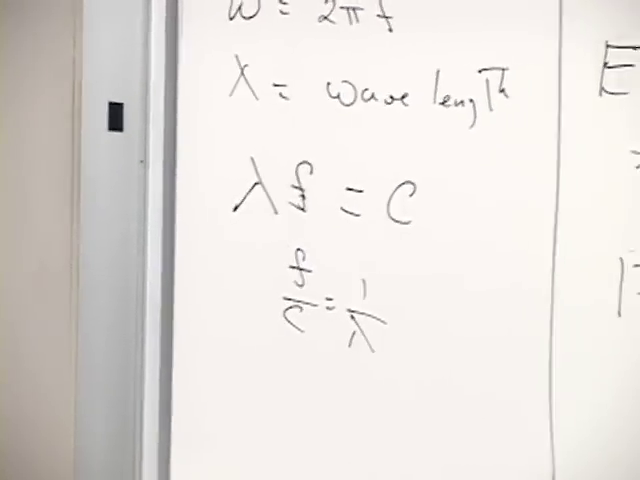
\includegraphics[width=0.56\textwidth]{lecture_02_figure_02.png}
\caption{بالنسبة إلى الضوء، \(\lambda f=c\) و\(f/c=1/\lambda\) هما العلاقتان المستخدمتان لاستخراج \(|\vec p_\gamma|=h/\lambda\).}
\lectureframe{00:21:39}
\end{figure}

كلما قصر الطول الموجي، ازداد زخم الفوتون. وهذه إحدى أهم الحقائق الكمومية في فيزياء الجسيمات. فلدراسة جسم صغير يحتاج المرء إلى مسبار قصير الطول الموجي، وثمن ذلك القِصر في الطول الموجي هو زخم كبير.

\begin{classroomqa}
\lecturetimestamp{00:22:23}
\audiencequestion{هل \(E=\hbar\omega\) أساسي، أم إنه مشتق من مبدأ أعمق؟}
\lecturerresponse{ينتج ذلك من ميكانيكا الكم للمذبذب التوافقي. وستُستخدم هذه النتيجة هنا من دون إعادة برهانها؛ وتوفّر لغة المذبذب التي ستُطوَّر أدناه الإطار الأعمق لها.}
\end{classroomqa}


\section{سعة الموجة وعدد الفوتونات}

\begin{classroomqa}
\lecturetimestamp{00:23:10}
\audiencequestion{ماذا تعني سعة الموجة بلغة الفوتونات؟}
\lecturerresponse{قارن بين موجتين لهما الطول الموجي والتردد نفسيهما ولكن بسعتين مختلفتين، مثل \(\sin(kx)\) و\(A\sin(kx)\). وكلاسيكيًا، تكون الطاقة في منطقة ثابتة متناسبة مع مربع السعة. وكموميًا، يكون للنمط الذي يحتوي على \(n\) فوتونًا طاقة \(n\hbar\omega\). ولذلك، عند تثبيت التردد والمنطقة والتطبيع، تنمو السعة، من حيث رتبة المقدار، مثل \(\sqrt n\).}
\end{classroomqa}

الموجتان متماثلتان في نمط تذبذبهما. وإحداهما ببساطة أشد من الأخرى.\footnote{يوضّح الرسم التخطيطي مقارنة الموجتين عند 00:23:47--00:24:28.}

\begin{figure}[t]
\centering
\begin{tikzpicture}[x=1cm,y=0.65cm]
\draw[->] (-0.4,0) -- (6.8,0);
\draw[->] (-0.4,-2.1) -- (6.8,-2.1);
\draw[thick] plot[domain=0:6.2,samples=120] (\x,{0.45*sin(\x r)});
\draw[thick] plot[domain=0:6.2,samples=120] (\x,{-2.1+1.15*sin(\x r)});
\draw (6.2,0.55) node[right]{small amplitude};
\draw (6.2,-0.75) node[right]{large amplitude};
\end{tikzpicture}
\caption{موجات لها الطول الموجي والتردد نفسيهما ولكن بسعات مختلفة.}
\end{figure}

لمقدار ثابت من الموجة،
\begin{equation}
E_{\text{wave}}\propto A^2.
\end{equation}
وبالنسبة إلى موجة كهرومغناطيسية، فهذا هو القول المألوف إن طاقة الحقل تتناسب مع مربع شدة الحقل. وإذا احتوى النمط نفسه على \(n\) فوتونًا، فإن
\begin{equation}
E_{\text{wave}}=n\hbar\omega.
\end{equation}
وبالتالي، مع تثبيت النمط والتردد والتطبيع والمنطقة،
\begin{equation}
A^2\propto n\hbar\omega,
\qquad
A\propto\sqrt n\quad\text{at fixed }\omega.
\end{equation}
ولا يُدَّعى هنا أي تطبيع دقيق. فمقدار الموجة المشمول مهم: إذ إن مضاعفة طول موجة منتظمة فيما عدا ذلك تغيّر طاقتها الكلية من دون أن تغيّر السعة الموضعية. ولذلك يمكن فهم التناسب على أنه يخص منطقة ثابتة، مثل طول موجي واحد.

وهناك أيضًا تحفّظ كمّي مخصوص. فلا يمكن إسناد قيم كلاسيكية مضبوطة تمامًا إلى السعة والطور معًا. ولذلك يكون السؤال ``ما سعة فوتون واحد؟'' ملتبسًا إذا كان يطلب حقلًا كلاسيكيًا محددًا على نحو حاد تمامًا. ومع ذلك، فإن اتخاذ \(n=1\) يعطي مقياسًا معقولًا لرتبة المقدار.

\begin{classroomqa}
\lecturetimestamp{00:28:25}
\audiencequestion{هل تمثّل الإزاحة العمودية في رسم موجة كهرومغناطيسية موضع الفوتون في الفضاء؟}
\lecturerresponse{لا. فمحور الانتشار مكاني، في حين يمثّل الإحداثي العمودي قيمة المجال الكهربائي أو المغناطيسي. ويتجه الزخم على طول محور الانتشار، لا على طول سعة الحقل المرسومة.}
\end{classroomqa}

قد تنتشر الموجة في أي اتجاه مكاني، لكن الرسم الجيبي المألوف يستخدم محوره الأفقي وحده بوصفه إحداثيًا مكانيًا. أما الاتجاه الآخر المرسوم فيسجّل شدة الحقل.

\begin{classroomqa}
\lecturetimestamp{00:29:37}
\audiencequestion{هل يُعَدّ عدد الفوتونات المذكور داخل طول موجي واحد أم داخل دورة واحدة من الموجة؟}
\lecturerresponse{يمكن اختيار منطقة ثابتة، مثل طول موجي واحد. ولهذا فالعلاقة تناسبية فحسب: إذ تعتمد الطاقة الكلية وعدد الفوتونات أيضًا على مقدار ما يُضمَّن من الموجة. فطولان موجيان أو ثلاثة أو أربعة أطوال موجية تحتوي، عند السعة نفسها، على طاقة أكبر تبعًا لذلك من طول موجي واحد.}
\end{classroomqa}

\begin{classroomqa}
\lecturetimestamp{00:30:17}
\audiencequestion{هل سعة فوتون واحد بلا معنى؟}
\lecturerresponse{لا تكون ذات معنى إلا بوصفها عبارة عن رتبة مقدار تُستحصل بوضع \(n=1\). بالنسبة إلى نمط كهرومغناطيسي، تؤدي معلومات المجالين الكهربائي والمغناطيسي دورًا مماثلًا لمعلومات الموضع والزخم المترافقين، لذا يحد عدم اليقين الكمومي من مدى إمكان تعيين سعة كلاسيكية تعيينًا حادًا. وتظل علاقة رتبة المقدار مفيدة.}
\end{classroomqa}

تقود هذه الأسئلة بالفعل إلى نظرية الحقل الكمومي، حيث يمكن بيان العلاقة بين متغيرات الحقل وعدد الجسيمات على نحو دقيق. أما الآن فتكفي علاقات التناسب.

\section{العلاقات الكمومية العامة وموجات المادة البطيئة}

تنطبق بعض الصيغ التي قُدِّمت للفوتونات على نحو أعم بكثير، بينما لا تنطبق صيغ أخرى كذلك. ومن المفيد فرزها قبل الانتقال إلى الإلكترونات.

\begin{figure}[t]
\centering
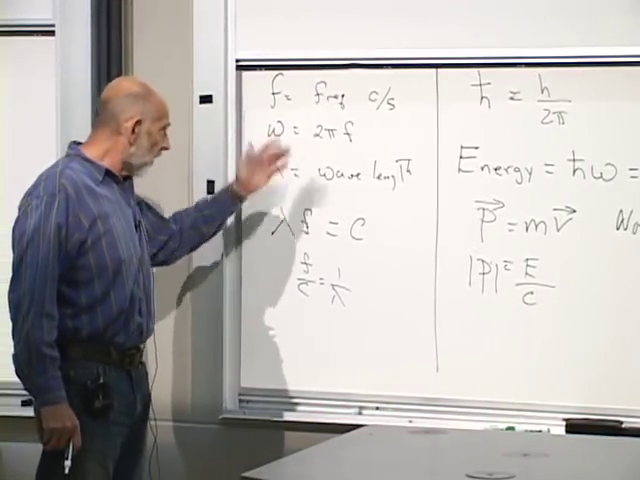
\includegraphics[width=0.82\textwidth]{lecture_02_figure_03.png}
\caption{تعريفات الموجات، وعلاقتا الزخم للفوتون وللحركة غير النسبية، مقارنةً بحسب مجالات صلاحيتهما.}
\lectureframe{00:31:52}
\end{figure}

تنطبق تعريفات \(f\) و\(\omega=2\pi f\) و\(\lambda\) على نحو عام. كما أن العلاقة الكمومية
\begin{equation}
E=\hbar\omega=hf
\end{equation}
عامة أيضًا في المناقشة الحالية. وعلى النقيض من ذلك، فإن الصيغ التي تتضمن \(c\)، مثل \(\lambda f=c\) و\(|\vec p|=E/c\)، تنطبق على الموجات التي تتحرك بسرعة الضوء. أما الصيغة \(\vec p=m\vec v\) فتنطبق على الجسيمات التي تتحرك أبطأ بكثير من الضوء. وتتطلب الحركة النسبية بين هذين الحدين استيفاءً ليس مطلوبًا بعد.

لا تقتصر علاقة الزخم--الطول الموجي على مثال الفوتون:
\begin{equation}
p=\frac{h}{\lambda}.
\end{equation}
وهنا يدل \(p\) على المقدار عندما تُؤخذ \(\lambda\) بوصفها طولًا موجيًا موجبًا؛ ويمكن تحديد الاتجاه على نحو منفصل.

\begin{figure}[t]
\centering
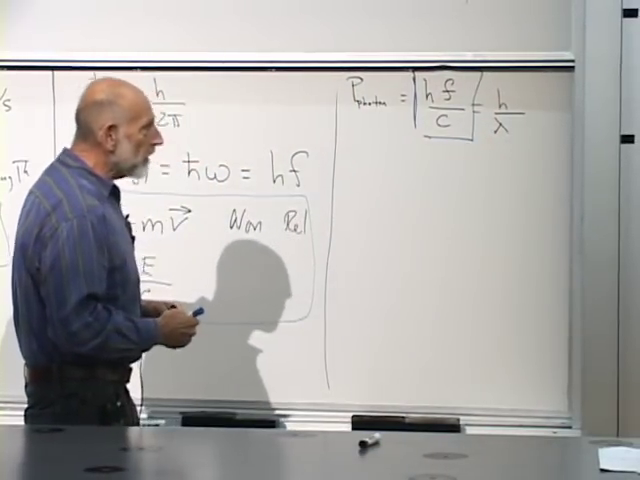
\includegraphics[width=0.74\textwidth]{lecture_02_figure_04.png}
\caption{زخم الفوتون \(|\vec p_\gamma|=hf/c=h/\lambda\)، مما يقود إلى علاقة دي برولي العامة.}
\lectureframe{00:33:32}
\end{figure}

يمكن ربط إلكترون، ونواة، وحتى كرة بولينغ، بموجة. ويُعد تداخل الإلكترونات أحد تجليات هذه الحقيقة. اكتب موجة الإلكترون على الصورة \(\psi\). ما الذي يحل محل \(\lambda f=c\) لإلكترون يتحرك ببطء؟ العنصر الناقص هو العلاقة غير النسبية بين الطاقة والزخم.

نبدأ بالطاقة الحركية والزخم:
\begin{align}
E&=\frac12 mv^2,\\
p&=mv,
\qquad
v=\frac{p}{m}.
\end{align}
وبالتعويض من العلاقة الأخيرة في الأولى نحصل على
\begin{align}
E
&=\frac12m\left(\frac{p}{m}\right)^2\\
&=\frac{p^2}{2m}.
\end{align}
تظهر الكتلة في البسط في \(\frac12 mv^2\) وفي المقام في \(p^2/(2m)\). ومن السهل الالتباس في هذا الترتيب، ومن المفيد إعادة اشتقاقه.

والآن نستخدم العلاقات الكمومية العامة
\begin{equation}
E=hf,
\qquad
p=\frac{h}{\lambda}.
\end{equation}
وبالنسبة إلى جسيم بطيء واحد،
\begin{align}
hf
&=\frac{p^2}{2m}\\
&=\frac{1}{2m}\left(\frac{h}{\lambda}\right)^2\\
&=\frac{h^2}{2m\lambda^2}.
\end{align}
وبالقسمة على \(h\) نحصل على
\begin{equation}
f=\frac{h}{2m\lambda^2}.
\end{equation}

\begin{figure}[t]
\centering
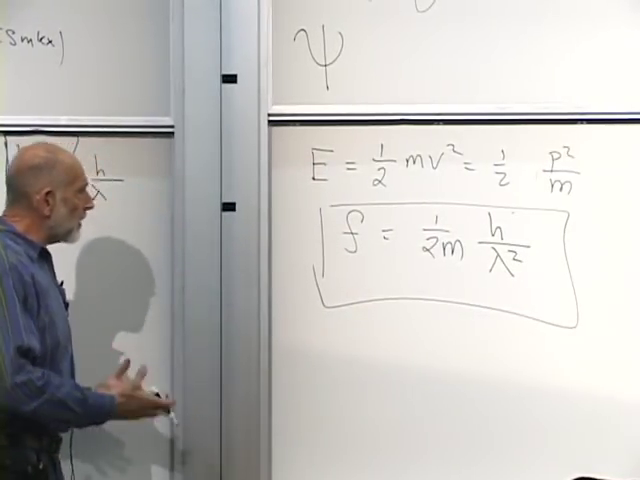
\includegraphics[width=0.64\textwidth]{lecture_02_figure_05.png}
\caption{بالنسبة إلى جسيم بطيء، تؤدي \(E=p^2/(2m)\) و\(p=h/\lambda\) إلى \(f=h/(2m\lambda^2)\).}
\lectureframe{00:37:47}
\end{figure}

بالنسبة إلى الضوء،
\begin{equation}
f\propto\frac{1}{\lambda},
\end{equation}
أما بالنسبة إلى المادة البطيئة،
\begin{equation}
f\propto\frac{1}{\lambda^2}.
\end{equation}
فلا حاجة إلى حفظ العلاقة الثانية بمعزل عن غيرها. إذ يمكن دائمًا إعادة بنائها انطلاقًا من \(E=p^2/(2m)\) و\(E=hf\) و\(p=h/\lambda\). وبالنسبة إلى إلكترون يتحرك ببطء في ذرة، فإنها تعطي تردد موجة Schr\"odinger الموافقة.

\begin{classroomqa}
\lecturetimestamp{00:38:35}
\audiencequestion{هل تنطبق علاقة التردد--الطول الموجي غير النسبية على جسيمات أخرى غير الإلكترونات؟}
\lecturerresponse{نعم. إنها تنطبق على أي جسيم يتحرك أبطأ بكثير من الضوء. أما الاستيفاء النسبي بين الحد البطيء والحد الضوئي فهو موضوع مستقل.}
\end{classroomqa}

\begin{classroomqa}
\lecturetimestamp{00:38:55}
\audiencequestion{ما العلاقة التي تنطبق على نيوترينو؟}
\lecturerresponse{يعتمد ذلك على سرعة النيوترينو. فمعظم النيوترينوهات التي نصادفها في الطبيعة تتحرك بسرعة قريبة جدًا من سرعة الضوء، لذا تكون علاقة الحد الضوئي تقريبًا جيدًا. أما النيوترينو الذي يتحرك أبطأ بكثير من الضوء فيخضع بدلًا من ذلك للعلاقة غير النسبية.}
\end{classroomqa}

\editorialnote{يتناول تبادل قصير مع الحضور، مباشرة بعد سؤال النيوترينو، السعات والكمّات واختلاف الأطوال الموجية للإلكترونات، لكن صياغته متضررة أكثر مما يسمح باستعادتها على نحو موثوق. أما الرد الذي أمكن استخلاصه فيؤجل العلاقة العامة بين السعات والكمّات ذات الأطوال الموجية المختلفة.}

\begin{classroomqa}
\lecturetimestamp{00:39:56}
\audiencequestion{هل يكون إلكترون من مسرّع \(20\,\mathrm{keV}\) بطيئًا أم نسبيًا؟}
\lecturerresponse{يُعامل على أنه بطيء. ففي الوحدات التي يكون فيها \(c=1\)، يمكن التعبير عن الكتلة والطاقة والزخم بالوحدات نفسها. ويبلغ مقياس طاقة السكون للإلكترون تقريبًا \(0.5\,\mathrm{MeV}\)، في حين أن \(20\,\mathrm{keV}\) أصغر بكثير. وبصورة مكافئة، فإن معيار الزخم غير النسبي هو \(p\ll mc\).}
\end{classroomqa}

مقارنة الطاقة في المثال هي
\begin{equation}
K=20\,\mathrm{keV}\ll m_ec^2\simeq0.5\,\mathrm{MeV}.
\end{equation}
\editorialnote{يعرض المقطع الأصلي عند 00:39:56--00:41:40 القيمة \(20\,\mathrm{keV}\) بوصفها طاقة مسرّع، ثم يصوغ المعيار النسبي بدلالة مقارنة الزخم بكتلة السكون. إن كتابة معياري الطاقة الحركية والزخم كلٌّ على حدة تتجنب مساواة الطاقة المذكورة بزخم، مع الحفاظ على الاستنتاج غير النسبي المذكور.}

\section{سرعة الطور، وسرعة المجموعة، والتشتت}

\begin{classroomqa}
\lecturetimestamp{00:41:46}
\audiencequestion{هل يمكن استخدام حاصل ضرب التردد في الطول الموجي للحصول على سرعة موجة إلكترون؟}
\lecturerresponse{إنه يعطي سرعة الطور، لا السرعة المنسوبة إلى الإلكترون. وللحزمة الموضعية كلٌّ من سرعة طور تصف حركة قممها وقيعانها الداخلية، وسرعة مجموعة تصف حركة الغلاف. وتُعرَّف سرعة المجموعة بأنها السرعة الموافقة لحركة الجسيم.}
\end{classroomqa}

تبدو الحزمة الموجية محليًا كموجة جيب أو جيب تمام، لكنها محصورة بغلاف. وأثناء حركتها، لا يلزم أن يتحرك الغلاف والقمم الموجودة داخله بالسرعة نفسها.\footnote{يتبع هذا الرسم التخطيطي مناقشة الحزمة الموجية عند 00:42:34--00:44:11.}

\begin{figure}[t]
\centering
\begin{tikzpicture}[x=0.75cm,y=0.8cm]
\draw[->] (-0.5,0) -- (12.8,0);
\draw[thick] plot[domain=0:12,samples=140] (\x,{1.10*exp(-0.20*(\x-6)^2)});
\draw[thick] plot[domain=0:12,samples=140] (\x,{-1.10*exp(-0.20*(\x-6)^2)});
\draw[thick] plot[domain=0:12,samples=240] (\x,{1.10*exp(-0.20*(\x-6)^2)*sin(6*\x r)});
\draw[->] (4.1,1.45) -- (7.5,1.45);
\draw (5.8,1.8) node{group motion};
\draw[->] (7.0,-1.55) -- (8.3,-1.55);
\draw (8.7,-1.55) node[right]{phase motion};
\end{tikzpicture}
\caption{حزمة موجية موضعية يتحرك غلافها وطورها الداخلي عمومًا بسرعات مختلفة.}
\end{figure}

سرعة الطور هي سرعة القمم والقيعان وسائر الأطوار الثابتة لمركبة وحيدة التردد. وبالنسبة إلى علاقة التشتت غير النسبية،
\begin{equation}
v_\phi=f\lambda=\frac{h}{2m\lambda}.
\end{equation}
فهي تعتمد على الطول الموجي. ولذلك تكون لمركبات الأطوال الموجية المختلفة سرعات طور مختلفة، ومن ثم يمكن للقمم أن تتحرك عبر الحزمة ويمكن للحزمة أن تتشتت. أما سرعة المجموعة فهي سرعة الحزمة ككل، وهي التي تُعرَّف بوصفها سرعة الجسيم.

توجد حالة خاصة بسيطة. فإذا تحركت جميع مركبات الأطوال الموجية بالسرعة نفسها، اتفقت سرعتا الطور والمجموعة. وللضوء في الفراغ هذه الخاصية: فكل طول موجي ينتشر بسرعة \(c\). أما علاقة الجسيم البطيء فلا تملكها؛ إذ إن \(f\lambda\) فيها يتغير مع \(\lambda\).

المعادلة
\begin{equation}
f=\frac{h}{2m\lambda^2}
\end{equation}
هي معادلة Schr\"odinger الحرة في صورة مموهة قليلًا. يحدد التردد الاعتماد الزمني لموجة مستوية، ويحدد الطول الموجي اعتمادها المكاني، وتربط معادلة Schr\"odinger بينهما. وعلى العكس، فإن إدخال موجة ذات تردد معيّن وطول موجي معيّن في معادلة Schr\"odinger الحرة يعيد إنتاج علاقة التشتت هذه.

\begin{classroomqa}
\lecturetimestamp{00:47:02}
\audiencequestion{هل يمكن أن تتجاوز سرعة الطور سرعة الضوء؟}
\lecturerresponse{نعم. سرعة الطور لا تنقل معلومات. أما المعلومات والحزمة الموضعية فتنتشران بسرعة المجموعة، لذا لا تتيح سرعة طور فوق ضوئية إرسال إشارات فوق ضوئية.}
\end{classroomqa}

\section{الفضاء المحدود والزخم المتقطع}

الغاية النهائية هي الموجات في فضاء لانهائي، لكن البدء بنظام محدود أكثر أمانًا. فاللانهاية ليست شيئًا يستطيع الحاسوب تخزينه أو معالجته مباشرة. تُصاغ المعادلات أولًا لنظام محدود، ثم لا يُؤخذ إلا بعد ذلك الحد الذي يصبح فيه حجمه كبيرًا كيفما نشاء. وهذه العادة مفيدة في ميكانيكا الكم، ونظرية الحقل الكمومي، وفيزياء الجسيمات كلها.

لا يضيع شيء أساسي بالبدء في بعد مكاني واحد. فقد تعيش الموجة على وتر كمان، أو على حبل يُهز، أو في عالم تجريدي أحادي البعد. وأوضح نظام محدود هو قطعة طولها \(L\) ذات طرفين عاكسين. تنتقل موجة إلى أحد الطرفين، فتنعكس، ثم تعود. هذا شرط حدود عاكس مشروع تمامًا، لكنه ينطوي على إزعاج: فالزخم غير محفوظ داخل النظام الموجي. فالموجة المتحركة نحو اليمين تحمل زخمًا يمينيًا؛ وبعد الانعكاس تحمل زخمًا يساريًا. وقد وفّر الحدّ الدفعة وامتص الفرق.

يمكن تمثيل انقلاب الزخم عند طرف عاكس تمثيلًا تخطيطيًا.\footnote{يتبع هذا الرسم التخطيطي الحجة المتعلقة بالحدود العاكسة عند 00:49:24--00:51:08.}

\begin{figure}[t]
\centering
\begin{tikzpicture}[x=1cm,y=1cm]
\draw[thick] (0,0) -- (7,0);
\draw[very thick] (0,-0.45) -- (0,0.45);
\draw[very thick] (7,-0.45) -- (7,0.45);
\draw[->,thick] (1.0,0.35) -- (5.8,0.35) node[midway,above]{\(p>0\)};
\draw[->,thick] (5.8,-0.35) -- (1.0,-0.35) node[midway,below]{\(p<0\)};
\draw (3.5,-0.85) node{\(L\)};
\end{tikzpicture}
\caption{الانعكاس عند طرفي قطعة محدودة يقلب اتجاه زخم موجة منتقلة.}
\end{figure}

هناك طريقة أخرى لجعل النظام منتهيًا مع الحفاظ على الزخم. اجعل طرفي القطعة متطابقين. يمكن رسم النتيجة على هيئة دائرة، لكن لا حاجة إلى دائرة حرفية مضمَّنة في بُعد ثانٍ. والصياغة الرياضية هي ببساطة أن الإحداثي دوري: فبعد قطع مسافة كلية مقدارها \(L\) يعود المرء إلى النقطة نفسها.

\begin{figure}[t]
\centering
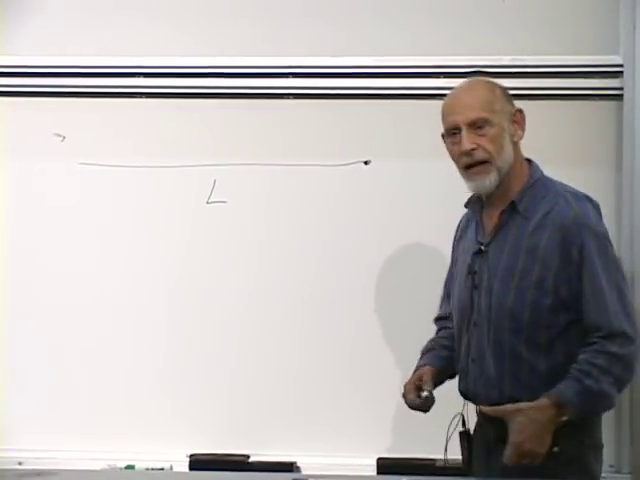
\includegraphics[width=0.72\textwidth]{lecture_02_figure_06.png}
\caption{مسار أحادي البعد بطول كلي \(L\) يُستخدم لتقديم المطابقة الدورية.}
\lectureframe{00:51:21}
\end{figure}

يُصرَّح بتطابق الطرفين في المخطط الآتي.\footnote{ويتبع هذا المخطط حجة المطابقة الدورية عند 00:51:09--00:52:37.}

\begin{figure}[t]
\centering
\begin{tikzpicture}[x=1cm,y=1cm]
\draw[thick] (0,0) -- (7,0);
\fill (0,0) circle (1.5pt);
\fill (7,0) circle (1.5pt);
\draw[->,thick] (1.0,0.35) -- (6.0,0.35);
\draw (3.5,-0.35) node{\(L\)};
\draw[->,bend left=45] (7,0.08) to (0,0.08);
\draw (3.5,1.2) node{identified endpoints};
\end{tikzpicture}
\caption{فضاء دوري أحادي البعد يتكون من مطابقة طرفي مسار طوله \(L\).}
\end{figure}

تصل موجة تتحرك إلى اليمين بعد ذلك إلى الطرف المبيَّن، ثم تظهر من جديد عند البداية وتواصل الحركة إلى اليمين. وبالمثل تواصل موجة تتحرك إلى اليسار الحركة إلى اليسار. ولا يوجد طرف مميَّز تنعكس عنده الموجة، لذا لا ينقلب الزخم. يجعل الفضاء الدوري الحجم منتهيًا ويحفظ الزخم، لكن له نتيجة مهمة: الزخوم المسموح بها متقطعة.

يجب أن ينطبق عدد صحيح من الأطوال الموجية على الطول الكلي. وبالنسبة إلى نمط غير ثابت،
\begin{equation}
\lambda_{|N|}=\frac{L}{|N|},
\qquad |N|=1,2,3,\ldots .
\end{equation}
وبالتالي يمكن أن يكون مقدار الطول الموجي \(L\) أو \(L/2\) أو \(L/3\)، وهكذا. أما اختيار مثل \(L/\sqrt{2}\) فلا ينطبق: فبعد دورة كاملة ستعود الموجة بطور غير صحيح ولن تطابق قيمتها الابتدائية.

باستخدام \(p=h/\lambda\)، يكون مقدار الزخم للنمط غير الثابت ذي الرتبة \(|N|\) هو
\begin{equation}
|p_N|=\frac{|N|h}{L}.
\end{equation}
ولإدخال الاتجاهين معًا والنمط الثابت بلا لبس، من الملائم أن يكون دليل النمط ذا إشارة:
\begin{equation}
p_N=\frac{Nh}{L},
\qquad N=0,\pm1,\pm2,\ldots .
\end{equation}
وتصف القيم الموجبة والسالبة لـ \(N\) اتجاهي انتشار متعاكسين. أما النمط \(N=0\) فهو ثابت وزخمه صفري؛ وليس له طول موجي متناهٍ يُدرج في \(h/\lambda\). ولذلك يكون التباعد الأساسي في الزخم هو \(h/L\).

عندما يكون \(L\) عيانيًا، فإن كِلًا من \(h\) و\(1/L\) يجعل هذا التباعد صغيرًا للغاية، بحيث تشكّل القيم المسموح بها مجموعة كثيفة جدًا وتبدو شبه متصلة. ومع ذلك فإن خرزةً مقيَّدة بسلك دائري تمتلك بالضبط هذا الطيف المتقطّع.

\begin{classroomqa}
\lecturetimestamp{00:58:27}
\audiencequestion{هل الكمية المتكمّاة هي الزخم الكلي للموجة، أم الزخم المرتبط بدورة واحدة؟}
\lecturerresponse{تنطبق هذه العبارة على زخم كل كمّ. فلكل كمّ أحد الزخوم المتقطعة المسموح بها. وبالتالي فإن الزخم الكلي لأي مجموعة من الكمّات يكون أيضًا مضاعفًا صحيحًا للوحدة الأساسية \(h/L\).}
\end{classroomqa}

\begin{classroomqa}
\lecturetimestamp{00:59:22}
\audiencequestion{لماذا يجب أن تعود الموجة إلى القيمة نفسها بعد دورة كاملة؟}
\lecturerresponse{الطرفان المتطابقان هما النقطة الفيزيائية نفسها، لذلك يجب أن يكون للحقل القابل للرصد القيمة نفسها عندهما. وأي عدم تطابق سيتطلب قفزة مفاجئة في الحقل عند تلك النقطة. ومثل هذا الانقطاع مكلف من حيث الطاقة والزخم؛ لذا فإن تشكيلات الحقل المسموح بها متصلة ودورية.}
\end{classroomqa}

\begin{classroomqa}
\lecturetimestamp{01:00:09}
\audiencequestion{ماذا يحدث إذا كانت الموجة موضعية في حزمة؟}
\lecturerresponse{الحزمة مجموع فورييه من موجات مستوية، أو بصورة مكافئة من جيوب وجيوب تمام. وفي الفضاء الدوري لا يجوز أن يحتوي هذا المجموع إلا على أنماط الزخم المتقطعة المسموح بها. لذا فإن عبارة التكميم هي عبارة عن مركبات فورييه لكل حزمة مسموح بها.}
\end{classroomqa}

\begin{classroomqa}
\lecturetimestamp{01:01:01}
\audiencequestion{هل توجد مشكلة إذا صار الطول الدوري \(L\) صغيرًا للغاية؟}
\lecturerresponse{كلما تناقص \(L\)، ازداد الزخم الأساسي \(h/L\) كثيرًا. ولا يترتب على ذلك أي عدم اتساق فوري عند الأطوال المجهرية المعتادة، لكن محاولة دفع هذا البناء إلى نطاق طول بلانك يُتوقع أن تتطلب فيزياء جديدة.}
\end{classroomqa}

الآن خذ الصورة الدائرية على نحو حرفي: تتحرك خرزة على سلك دائري نصف قطره \(r\)، ومحيطه \(L=2\pi r\). وزخومها المماسية المسموح بها هي
\begin{equation}
p_N=\frac{Nh}{2\pi r}=\frac{N\hbar}{r}.
\end{equation}
وبالنسبة إلى جسيم غير نسبي في مدار دائري، يكون العزم الزاوي هو \(mvr\). وبما أن \(p=mv\) في ذلك النظام، فهذا يساوي \(rp\). والتعبير \(mvr\) ليس عامًّا نسبيًا، لأن \(p\) عندئذٍ لا يساوي ببساطة \(mv\)، لكن حاصل ضرب الزخم في المسافة العمودية يظل العلاقة الصحيحة. وفي الصورة المتجهية،\footnote{تستعمل المحاضرة أولًا \(L\) للعزم الزاوي، ثم تنتبه إلى تعارضه مع \(L\) للطول الدوري فتغيّر الرموز. وهنا يُستعمل \(J\) على امتداد النص؛ انظر 01:03:40--01:05:21.}
\begin{equation}
\vec J=\vec r\times\vec p,
\end{equation}
وللحركة الدائرية المماسية يكون مقداره \(J=rp\). ومن ثم
\begin{equation}
J_N=rp_N=N\hbar.
\end{equation}
يعتمد تباعد الزخم الخطي على حجم الدائرة، في حين أن وحدة العزم الزاوي هي دائمًا \(\hbar\). وتوجد استثناءات لقاعدة العدد الصحيح عندما تكون الفرميونات داخلة في المسألة؛ وتؤجَّل تلك الاستثناءات.

المهمة التالية هي ربط الحقول بالجسيمات والكمّات على نحو أدق. وهذا يتطلب عودة قصيرة إلى ميكانيكا الكم الخاصة بالمؤثرات والمذبذب التوافقي.

\section{أنماط الموجة والمؤثرات الكمومية}

إن ميكانيكا الكم الآتية لا بد أن تكون مجردة، والمقصود بها المراجعة. والمذبذب التوافقي هو النظام الأساسي لأن الموجة اهتزاز. فعند نقطة ثابتة، يتغير المجال الكهربائي أو المجال المغناطيسي أو أي سعة موجية أخرى دوريًا مع الزمن؛ والقول إن لمركبة ما ترددًا هو في ذاته قول إنها تتذبذب.

لا يلزم أن تكون للموجة العامة طول موجي واحد فقط. إذ يمكن مزج ضوء من عدة ألوان معًا، وبالعكس يمكن لمنشور أن يفصل الضوء المختلط إلى ألوانه المكوِّنة، كما في تحليل Newton للضوء الأبيض. ولكل مركبة طول موجي وتردد وسعة وطاقة وزخم خاص بها. ومن ثم يمكن تحليل الموجة المختلطة إلى كمّات ذات طاقات وزخوم مختلفة. وكل طول موجي يحدد ترددًا، وكل مركبة ذات تردد محدد تسلك سلوك مذبذب. ولهذا كان المذبذب التوافقي، لا أي نظام كمومي اعتباطي، هو اللبنة الأساسية الطبيعية للحقل.

تُمثَّل المرصودات الكمومية بالمؤثرات. ويمكن جمع المؤثرات وضربها، لكن بخلاف الأعداد العادية لا يلزم أن تكون نواتج ضربها مستقلة عن الترتيب. ولتُمثِّل \(A\) و\(B\) خاصيتين لنظام ما، يمكن أن تكون كل منهما قابلة للقياس بمفردها. فعلى سبيل المثال، قد تمثل \(A\) مجالًا كهربائيًا وتمثل \(B\) مجالًا مغناطيسيًا. وإذا كانت القيم المقاسة هي العددين العاديين \(a\) و\(b\)، فإن
\begin{equation}
ab=ba.
\end{equation}
فلا يمكن أن يعتمد حاصل ضربهما العددي على ترتيب الضرب. غير أن المؤثرات المناظرة في ميكانيكا الكم قد تحقق بدلًا من ذلك \(AB-BA\neq0\).

في البداية يبدو هذا غير معقول. فإذا كان قياس المجال الكهربائي يعطي عددًا ما وكان قياس المجال المغناطيسي يعطي عددًا آخر، فلا بد أن يعطي ضرب هذين العددين النتيجة نفسها بأي ترتيب. وحل ذلك هو أنه عندما تعتمد حواصل ضرب المؤثرات على الترتيب، لا يمكن قياس الكميتين معًا في الوقت نفسه. فالتجربة التي تقيس إحداهما تتداخل مع قياس الأخرى. ولا يوجد تناقض، لأن القيمتين العدديتين لا يمكن الحصول عليهما معًا.

عندما يمكن قياس كميتين معًا، تكون قيمتاهما المقاسوَتان عددين عاديين، وهذه الأعداد تتبادل الضرب. ولذلك فإن اختبار إمكان القياس المتزامن هو المبدّل
\begin{equation}
[A,B]=AB-BA.
\end{equation}
ويعني انعدام المبدّل أن المرصودات متوافقة؛ ويعني كون المبدّل غير صفري أن القياسات المناظرة تتداخل. وعكس ترتيب المدخلين يعكس الإشارة:
\begin{equation}
[B,A]=-[A,B].
\end{equation}

بالنسبة إلى جسيم غير نسبي، تتبادل مركبات الموضع الثلاث فيما بينها، وكذلك مركبات الزخم الثلاث:
\begin{align}
[x,y]&=[y,z]=[z,x]=0,\\
[p_x,p_y]&=[p_y,p_z]=[p_z,p_x]=0.
\end{align}
ويمكن تعيين الإحداثيات الثلاثة معًا، ويمكن تعيين مركبات الزخم الثلاث كلها معًا. أما مركبات الموضع والزخم المتناظرة فلا تتبادل الضرب:
\begin{equation}
[x,p_x]=[y,p_y]=[z,p_z]=i\hbar,
\end{equation}
في حين أن المركبات المختلطة مثل \([x,p_y]\) تنعدم. إن قياس إحداثي موضع يُحدث في الجسيم اضطرابًا في الزخم المقترن به. وبصورة مكافئة، فإن حاصل ضرب لا يقينَي الموضع والزخم المناظرين يضبطه \(\hbar\).

\begin{classroomqa}
\lecturetimestamp{01:16:30}
\audiencequestion{عند الانتقال من \(x\) إلى \(y\)، هل ينبغي أن تتغير \(i\) في المبدّل إلى \(j\)؟}
\lecturerresponse{لا. فالرمز \(i\) هو دائمًا الوحدة التخيلية، أي الجذر التربيعي لسالب واحد. وليس هو لا رمزًا لمتجهة وحدة ديكارتية ولا واحدًا من الرموز الكواتيرنيونية \(i,j,k\).}
\end{classroomqa}

\begin{classroomqa}
\lecturetimestamp{01:17:24}
\audiencequestion{هل يعني \(AB-BA\) قياس \(A\) أولًا ثم \(B\)، ثم عكس ترتيب القياس؟}
\lecturerresponse{لا. فالحدّان هما حاصل ضرب مؤثِّرات أو مصفوفات بترتيبين جبريين مختلفين. وهما لا يدلان على تتابع فعلي للقياسات. والارتباط بالقياسات غير المتوافقة هو نتيجة لجبر المؤثِّرات، لا لتعريف الجداء.}
\end{classroomqa}

\begin{classroomqa}
\lecturetimestamp{01:18:32}
\audiencequestion{هل تنطبق مبدِّلات الموضع--الزخم هذه مباشرةً على فوتون؟}
\lecturerresponse{ليس مباشرةً. فهي تنطبق بوضوح على الجسيمات غير النسبية. أما موضع الفوتون فأصعب تعريفًا، ولذلك تتطلب العبارة المناظرة مزيدًا من العناية، ولا نحتاج إليها هنا.}
\end{classroomqa}

\section{المذبذب التوافقي الكمومي}

يوفّر ثقل معلّق بنابض، وموجة صوتية، وموجة ضوئية، أمثلةً كلّها على الحركة الاهتزازية. ولكل مذبذب توافقي مثالي تردد. وبالنسبة إلى النابض، فالدورة الكاملة ليست مجرد الزمن اللازم لعودة الثقل إلى الموضع نفسه؛ بل يجب أن يعود إلى ذلك الموضع وهو يتحرك في الاتجاه نفسه. وعدد الدورات الكاملة في الثانية هو \(f\)، و\(\omega=2\pi f\).

في الوصف الكلاسيكي، يمكن للمذبذب المثالي أن يملك أي طاقة غير سالبة. فدفعة لطيفة تعطي طاقة صغيرة، ودفعة أشد تعطي طاقة أكبر. أما النابض الحقيقي فسينكسر أو ينصهر في النهاية، لكن المثال الرياضي المثالي له مجال متصل من الطاقات الموجبة. ويختلف المذبذب الكمومي: إذ تشكل طاقاته المسموح بها سُلّمًا منفصلًا متساوي التباعد. وإذا اختير مبدأ الطاقة بحيث يُسمّى أدنى مستوى صفرًا،
\begin{equation}
E_n=n\hbar\omega,
\qquad n=0,1,2,\ldots .
\end{equation}
ويمكن تصوير المستويات المتساوية التباعد كما يلي.\footnote{يتبع المخطط التخطيطي لمستويات الطاقة المناقشة على اللوح عند 01:21:20--01:23:56.}

\begin{figure}[t]
\centering
\begin{tikzpicture}[x=1cm,y=0.9cm]
\draw[->] (0,0) -- (0,5.35);
\draw (0,5.5) node[above]{energy};
\foreach \y/\lab in {0.6/{0},1.6/{\hbar\omega},2.6/{2\hbar\omega},3.6/{3\hbar\omega},4.6/{n\hbar\omega}}
{
  \draw[thick] (0.2,\y) -- (2.2,\y);
  \draw (-0.25,\y) node[left]{\(\lab\)};
}
\draw[->,thick] (2.8,0.68) -- (2.8,1.52);
\draw (3.2,1.1) node[right]{\(a_+\)};
\draw[->,thick] (3.7,1.52) -- (3.7,0.68);
\draw (4.1,1.1) node[right]{\(a_-\)};
\end{tikzpicture}
\caption{مستويات المذبذب المتساوية التباعد وفق الاصطلاح \(E_n=n\hbar\omega\).}
\end{figure}

إن التباعد \(\hbar\omega\) هو الطاقة نفسها التي أُسنِدت سابقًا إلى فوتون واحد ذي تردد زاوي \(\omega\). وقد تكون القيمة \(2\hbar\omega\) طاقة كمّ واحد ينتمي إلى مذبذب ذي تردد \(2\omega\)، أو طاقة كمّين في مذبذب ذي تردد \(\omega\). والتفسير الثاني هو المطلوب هنا. ويمكن لمذبذب واحد ذي تردد ثابت أن يحتوي صفرًا أو واحدًا أو اثنين أو ثلاثة أو أكثر من الكمّات، من دون أي طاقات مسموح بها بين الدرجات.

تُوسَم حالة المذبذب بالعدد الصحيح \(n\)، وتُكتب على هيئة كيت \(|n\rangle\). فالحالة \(|0\rangle\) هي الحالة الأرضية، و\(|1\rangle\) فيها كمّ إثارة واحد، و\(|2\rangle\) فيها كمّان، وهكذا. والكيت مجرد ترميز للحالة التي تؤثر فيها المؤثِّرات.

عرّف مؤثِّر رفع \(a_+\) يرفع الحالة مستوى واحدًا، ومؤثِّر خفض \(a_-\) ينزل بها مستوى واحدًا:
\begin{align}
a_+|n\rangle &= \sqrt{n+1}\,|n+1\rangle,\\
a_-|n\rangle &= \sqrt{n}\,|n-1\rangle.
\end{align}
وعوامل الجذر التربيعي العددية جزء من التعريفين. وعلى أدنى حالة،
\begin{equation}
a_-|0\rangle=0,
\end{equation}
لأنه لا توجد حالة تحت الحالة الأرضية.

من المهم هنا التمييز بين الأعداد العادية والمؤثِّرات. فالوسم \(n\) والمعاملات مثل \(\sqrt n\) هي أعداد عادية؛ وهي تتبادل مع كل شيء. أما الرمزان \(a_+\) و\(a_-\) فمؤثِّران، ويجب الحفاظ على ترتيبهما.

اخفض \(|n\rangle\) أولًا، ثم ارفعه من جديد. وتعطي خطوة الخفض
\begin{equation}
a_-|n\rangle=\sqrt n\,|n-1\rangle.
\end{equation}
ويضيف تأثير \(a_+\) على الحالة الناتجة عاملًا آخر هو \(\sqrt n\)، لأن رفع \(|n-1\rangle\) يعيدها إلى \(|n\rangle\):
\begin{align}
a_+a_-|n\rangle
&=a_+\bigl(\sqrt n\,|n-1\rangle\bigr)\\
&=\sqrt n\,\sqrt n\,|n\rangle\\
&=n|n\rangle.
\end{align}
وهكذا يقرأ \(a_+a_-\) رقم المستوى. فافترض مثلًا أن \(|\chi\rangle\) معلوم أنها حالة ذاتية للعدد، لكن وسم مستواها غير معلوم. فإذا كان
\begin{equation}
a_+a_-|\chi\rangle=q|\chi\rangle,
\end{equation}
فإن المعامل العددي العادي \(q\) هو عدد الكمّات في تلك الحالة. ولذلك يكون هذا الجداء هو مؤثِّر العدد،
\begin{equation}
\hat n=a_+a_-,
\end{equation}
وبحسب اصطلاح الطاقة المختار يكون الهاملتوني
\begin{equation}
H=\hbar\omega\,a_+a_-.
\end{equation}
وبالفعل فإن تأثيره على أي مستوى يعطي \(H|n\rangle=n\hbar\omega|n\rangle\).

والآن اعكس الترتيب. فالرفع أولًا يعطي \(\sqrt{n+1}|n+1\rangle\). ثم يعيد الخفض إلى \(|n\rangle\) ويعطي عاملًا ثانيًا \(\sqrt{n+1}\):
\begin{align}
a_-a_+|n\rangle
&=a_-\bigl(\sqrt{n+1}\,|n+1\rangle\bigr)\\
&=\sqrt{n+1}\,\sqrt{n+1}\,|n\rangle\\
&=(n+1)|n\rangle.
\end{align}
ويختلف الترتيبان بمقدار واحد على كل حالة، لذلك
\begin{equation}
[a_-,a_+]=a_-a_+-a_+a_-=1.
\end{equation}

للمذبذب كذلك سعة وطور. ويحدد طوره موضعه في دورته؛ وبصورة ملموسة، يمكن تثبيته بالزمن الذي يمر فيه المذبذب عبر الأصل في اتجاه مختار. وتأخير ذلك العبور يغيّر الطور من دون أن يغيّر التردد. وتجمع مؤثِّرات السلم المتغيرات الكمومية المرتبطة بالسعة والطور. وجبرها كمومي في جوهره، لكن فعلها بسيط: يضيف \(a_+\) كمًّا واحدًا من طاقة المذبذب ويزيل \(a_-\) كمًّا واحدًا. وبالنسبة إلى نمط كهرومغناطيسي، تكون تلك الكمّات فوتونات، ولذلك يسمّى المؤثِّران مؤثِّري الإنشاء والإفناء.

\begin{classroomqa}
\lecturetimestamp{01:37:34}
\audiencequestion{هل يقابل مؤثِّرا الرفع والخفض قياسًا فيزيائيًا؟}
\lecturerresponse{عدد الفوتونات قابل للقياس. أما المؤثِّران \(a_+\) و\(a_-\) فليسا مرصودين قابلين للقياس، كلٌّ على حدة، وذلك لأسباب تقنية إضافية. ويُظهر مبدّلهما أن الاثنين لا يتبادلان، لكن هذه الحقيقة وحدها ليست الحجة على أن أيًّا منهما، منفردًا، غير قابل للرصد.}
\end{classroomqa}

تعطي مجموعة من النوابض ذات الترددات الطبيعية المختلفة مذبذبات مستقلة كثيرة. وكذلك تفعل الأنماط الكهرومغناطيسية في تجويف: إذ يمكن إثارة طول موجي واحد من غير أن يُلزِم ذلك الأطوال الأخرى بأن تكون لها الإثارة نفسها. وكموميًا، تضيف مؤثِّرات الإنشاء والإفناء كمّات ذات تردد ثابت وتزيلها في كل مذبذب مستقل. وهذه اللغة مركزية لأن الجسيمات ستُعرَّف على أنها تلك الكمّات بالضبط.

\section{حقل بوصفه مجموعة من المذبذبات}

لنعد إلى فضاء دوري أحادي البعد طوله الكلي \(L\). ولأنماطه غير الثابتة مقادير أطوال موجية
\begin{equation}
\lambda_N=\frac{L}{N},
\qquad N=1,2,3,\ldots ,
\end{equation}
وترددات زاوية غير سالبة مناظرة \(\omega_N\). ولأجل المقارنة مع طيف الزخم السابق، من المفيد إعادة تسمية عدده الصحيح ذي الإشارة بـ \(M\):
\begin{equation}
p_M=\frac{Mh}{L},
\qquad M=0,\pm1,\pm2,\ldots .
\end{equation}
وتسجل إشارة \(M\) اتجاه الانتشار.
\editorialnote{عند 01:42:08--01:42:24، يُصحَّح دليل نمط التردد من مجال ذي إشارة إلى مجال يبدأ من الصفر صعودًا. ويُستعمل الرمز \(M\) هنا فقط للإبقاء على ترميز الزخم ذي الإشارة منفصلًا عن وسم نمط التردد غير السالب \(N\)؛ ولا يُدخل إشغالات مستقلة لكل من \(+M\) و\(-M\). وتبدأ قائمة المذبذبات غير الثابتة عند \(N=1\).}

يتصرف كل تردد مسموح به كمذبذب توافقي. ويمكن إضافة الطاقة على نحو مستقل إلى تردد واحد ثم إلى آخر. ويُرجأ المثال الأول المفصل لحقل كمومي إلى المحاضرة التالية، لكن ترميز الحالة واضح بالفعل. وبترتيب الأنماط غير الثابتة من أطول طول موجي فصاعدًا، اكتب
\begin{equation}
|n_1,n_2,n_3,\ldots\rangle,
\end{equation}
حيث إن \(n_N=0,1,2,\ldots\) هو عدد الكمّات في المذبذب ذي التردد \(\omega_N\). ويدل المدخل الأول على عدد الكمّات التي تشغل نمط أطول طول موجي، ويدل الثاني على عدد الكمّات التي تشغل النمط التالي، وهكذا إلى غير نهاية.

تجعل توافقيات الوتر هذا البناء ملموسًا. ويُعرض تخطيطيًا التدرج من النمط الأساسي إلى التوافقيين التاليين.\footnote{يتبع هذا الشكل التخطيطي مناقشة توافقيات الوتر عند 01:45:20--01:47:46.}

\begin{figure}[t]
\centering
\resizebox{\linewidth}{!}{%
\begin{tikzpicture}[x=0.98cm,y=1cm]
\draw[gray] (0,2.5) -- (6,2.5);
\draw[thick] plot[domain=0:6,samples=120] (\x,{2.5+0.48*sin(30*\x)});
\fill (0,2.5) circle (1.4pt);
\fill (6,2.5) circle (1.4pt);
\node[right] at (6.25,2.5) {fundamental: \(\omega_1\)};

\draw[gray] (0,1.25) -- (6,1.25);
\draw[thick] plot[domain=0:6,samples=120] (\x,{1.25+0.42*sin(60*\x)});
\fill (0,1.25) circle (1.4pt);
\fill (3,1.25) circle (1.4pt);
\fill (6,1.25) circle (1.4pt);
\node[right] at (6.25,1.25) {second harmonic: \(2\omega_1\)};

\draw[gray] (0,0) -- (6,0);
\draw[thick] plot[domain=0:6,samples=120] (\x,{0.42*sin(90*\x)});
\fill (0,0) circle (1.4pt);
\fill (2,0) circle (1.4pt);
\fill (4,0) circle (1.4pt);
\fill (6,0) circle (1.4pt);
\node[right] at (6.25,0) {third harmonic: \(3\omega_1\)};
\end{tikzpicture}%
}
\caption{النمط الأساسي للوتر وتوافقيه الثاني والثالث، مع عدم وجود عقد داخلية، ثم عقدة داخلية واحدة، ثم عقدتين داخليتين.}
\end{figure}

يتحرك النمط الأساسي على هيئة قوس عريض واحد، وليس له أي عقدة داخلية. وهو مذبذب واحد، وقد يكون عدد كمّاته \(n_1=0,1,2,\ldots\)؛ وتكلفة كل إثارة هي \(\hbar\omega_1\). وللتوافقي الثاني عقدة داخلية واحدة وتردده ضعف تردد النمط الأساسي. فإذا كان النمط الأساسي يصدر نغمة دو الوسطى، فإن هذا النمط يصدر نغمة دو على بعد أوكتاف أعلى. وله عدد إشغال مستقل \(n_2\)، وتكلفة كل كمّ من كمّاته هي \(\hbar\omega_2=2\hbar\omega_1\). أما التوافقي الثالث فله عقدتان داخليتان وثلاثة أمثال تردد النمط الأساسي. وله عدد إشغال مستقل خاص به \(n_3\)، ويمكن مرة أخرى أن يكون أي عدد صحيح غير سالب.

نمطًا بنمط، وفي اصطلاح الطاقة المستخدم أعلاه، تكون الطاقة مساوية لعدد الإشغال مضروبًا في طاقة الكم. وجمع هذه المساهمات يعطي
\begin{equation}
E=\sum_{N=1}^{\infty} n_N\hbar\omega_N.
\end{equation}
\editorialnote{هذا المجموع المعروض هو الجمع الجبري لطاقات الأنماط المذكورة كلٌّ على حدة عند 01:44:02--01:47:46.}

يجب تكرار رياضيات المذبذب التوافقي نفسها لكل نمط حقلي، مع مؤثِّر إنشاء واحد ومؤثِّر إفناء واحد لكل مذبذب مستقل. وفي هذا التصور الابتدائي الأول، يكون الحقل الكمومي هو تلك المجموعة الكاملة من المذبذبات وجبر الإنشاء--الإفناء الخاص بها.

هذه اللغة مكيَّفة مع تشتت الجسيمات. تدخل إلى التجربة كمّات ذات طاقة وزخم محددين، وتغادرها كمّات ذات طاقات وزخوم أخرى. تُزال الجسيمات الابتدائية بمؤثرات الإفناء؛ وتُدرَج الجسيمات الخارجة في الحالة النهائية بمؤثرات الخلق الخاصة بالأنماط المناسبة.

\begin{classroomqa}
\lecturetimestamp{01:49:38}
\audiencequestion{هل يُستعمل العدد الصحيح نفسه لوسم نمط المذبذب ولعدِّ عدد الكمّات فيه؟}
\lecturerresponse{هناك عددان صحيحان متميزان. فوسم النمط \(N\) يحدد النمط المكاني؛ وفي مثال الوتر، يحدد عددُ عُقَده التردد \(\omega_N\). أمّا عدد الإشغال \(n_N\) فيبيّن كم عددَ الكمّات التي لها ذلك التردد.}
\end{classroomqa}
\chapter{من أنماط الزخم إلى الحقول الكمومية المحلية}

ما الحقل الكمومي، وكيف يرتبط بالجسيمات؟ الأداة الرياضية الأساسية هي المهتز التوافقي. يحتوي الحقل على أنماط اهتزاز ممكنة كثيرة، ويعني تكميم الحقل تجميع مهتز توافقي كمومي واحد لكل نمط. ويسهل رؤية هذا البناء أولًا في فضاء دوري منتهٍ، حيث تكوّن الأنماط المسموح بها قائمة منفصلة.

\section{الفضاء الدوري وأعداد الموجة المسموح بها}

خذ إحداثيًا مكانيًا واحدًا \(x\)، واعتبر النقاط المفصولة بمسافة \(L\) متطابقة. ويمكن تصور الفضاء على أنه دائرة محيطها \(L\). وهذه حيلة مفيدة لحجم منتهٍ. ففي مجال منتهٍ له طرفان، تنعكس الموجة السائرة عن الطرفين. أما في مجال دوري فيمكنها أن تتابع سيرها في أي من الاتجاهين من دون انعكاس. ويُحفَظ تناظر الإزاحة، ومن ثم انحفاظ الزخم، بينما تُزال مؤقتًا تعقيدات الحجم اللانهائي.

للموجة المستوية الشكل
\begin{equation}
e^{ikx}.
\end{equation}
وبعد دورة واحدة حول الدائرة لا بد أن تعود إلى قيمتها الأصلية. وبما أن الموجة تساوي \(1\) عند \(x=0\)، فإن الدورية تقتضي
\begin{equation}
e^{ikL}=1.
\end{equation}
لماذا يحقق مضاعف صحيح لـ \(2\pi\) هذا الشرط؟ تعطينا صيغة أويلر
\begin{align}
e^{i2\pi n}
&=\cos(2\pi n)+i\sin(2\pi n)\\
&=1,
\qquad n\in\mathbb Z.
\end{align}
يكون جيب التمام مساويًا لـ \(1\) ويكون الجيب مساويًا لـ \(0\) بعد أي عدد صحيح من الدورات. ولذلك،
\begin{equation}
kL=2\pi n,
\qquad
k=\frac{2\pi n}{L},
\qquad n\in\mathbb Z.
\end{equation}
والكمية \(k\) هي عدد الموجة. أما العدد الصحيح \(n\) فيُعيّن عدد موجة مسموحًا؛ وهو لا يعدّ الجسيمات بعد.

يمكن التعبير عن الشرط نفسه بدلالة الطول الموجي. فالطول الموجي هو المسافة التي يتقدم خلالها الطور دورة كاملة، لذا
\begin{equation}
k\lambda=2\pi,
\qquad
k=\frac{2\pi}{\lambda}.
\end{equation}
فالطول الموجي الكبير يقابله عدد موجة صغير، والطول الموجي القصير يقابله عدد موجة كبير. ويقول شرط الدورية إن عددًا صحيحًا من الأطوال الموجية يلائم الالتفاف حول الدائرة.

بالنسبة إلى موجة كمومية، يكون الزخم
\begin{equation}
p=\frac{h}{\lambda}
=\frac{2\pi\hbar}{\lambda}
=\hbar k.
\end{equation}
ومن ثم فإن \(k\) و\(p\) لا يختلفان إلا بالعامل \(\hbar\). وتصف القيم الموجبة والسالبة لـ \(k\) موجات تتحرك في اتجاهين متعاكسين وجسيمات ذات زخم في اتجاهين متعاكسين. وفي الوحدات التي فيها \(\hbar=1\)، من الشائع أن يُسمّى \(k\) زخمًا من دون مزيد من التفريق.

لكل \(k\) مسموح قد يوجد عدد ما من الكمّات في ذلك النمط. وهذا يُدخل عددًا صحيحًا ثانيًا:
\begin{equation}
n(k)=\text{number of quanta with wave number }k.
\end{equation}
ويُسمّى هذا عدد الإشغال. فالعدد الصحيح في \(k=2\pi n/L\) يوسم النمط، أما \(n(k)\) فيبيّن كم جسيمًا يشغل ذلك النمط. ويجب إعطاء أعداد الإشغال للقيم السالبة من \(k\) كما للقيم الموجبة منه.

\begin{classroomqa}
\lecturetimestamp{00:11:58}
\audiencequestion{هل \(k\) نفسه عدد صحيح؟}
\lecturerresponse{لا. عدد الموجة هو مضاعف صحيح لـ \(2\pi/L\): \(k=2\pi n/L\). والعدد الصحيح \(n\) في تلك الصيغة يوسم قيمة الزخم المسموح بها، وهو متميز عن عدد الإشغال \(n(k)\)، الذي يعدّ الكمّات في النمط.}
\end{classroomqa}

\section{حالات عدد الإشغال ومؤثرات الأنماط}

الحالة الكمومية متجه، أو عنصر خطي. ويمكن جمع متجهات الحالات وضربها في أعداد، وتؤثر فيها المؤثرات لتنتج متجهات حالة أخرى. وتمثَّل الكميات الحقيقية القابلة للرصد بمؤثرات هيرميتية. وهذه الحقائق الأولية مهمة هنا لأن حالة متعددة الجسيمات والحقل سيُبنيان من تراكيب خطية ومؤثرات.

لتكن
\begin{equation}
k_j=\frac{2\pi j}{L},
\qquad j\in\mathbb Z.
\end{equation}
وسم مناسب لحالة متعددة الجسيمات هو السلسلة الكاملة لأعداد الإشغال. وباستخدام الاختصار \(n_j\equiv n(k_j)\) للمدخلات المعروضة، نكتب
\begin{equation}
\big|\{n(k_j)\}\big\rangle
=
\big|\ldots,n_{-2},n_{-1},n_0,n_1,n_2,\ldots\big\rangle.
\end{equation}
ويمثل المدخل \(n(k_1)\) عدد الجسيمات في أول نمط ذي زخم موجب، ويمثل \(n(k_2)\) العدد في الثاني، وهكذا. وتمتد السلسلة بلا نهاية في الاتجاهين.

\begin{figure}[t]
\centering
\includegraphics[width=0.72\textwidth]{lecture_03_figure_02.png}
\caption{عدد الإشغال \(n(k)\) لنمط زخم مسموح.}
\lectureframe{00:15:04}
\end{figure}

كل نمط زخم هو مهتز توافقي. ولذلك فله مؤثر رفع ومؤثر خفض. والرمز المكتوب أولًا على صورة \(a^{+}(k)\) و\(a^{-}(k)\) سيُكتب على صورة \(a^\dagger(k)\) و\(a(k)\). وفعلهما هو
\begin{align}
a^\dagger(k)\big|\ldots,n(k),\ldots\big\rangle
&=
\sqrt{n(k)+1}\notag\\
&\quad{}\times
\big|\ldots,n(k)+1,\ldots\big\rangle,
\\
a(k)\big|\ldots,n(k),\ldots\big\rangle
&=
\sqrt{n(k)}\,
\big|\ldots,n(k)-1,\ldots\big\rangle.
\end{align}
يعمل المؤثر \(a^\dagger(k)\) على الخانة التابعة لـ \(k\)، فيرفع ذلك الإشغال بمقدار واحد، ويضرب الحالة في \(\sqrt{n(k)+1}\). ويخفض المؤثر \(a(k)\) الخانة نفسها ويعطي \(\sqrt{n(k)}\). ولكل زخم مسموح زوج كهذا.

\begin{figure}[t]
\centering
\includegraphics[width=0.58\textwidth]{lecture_03_figure_03.png}
\caption{مؤثرا الخلق والفناء المرتبطان بنمط الزخم \(k\).}
\lectureframe{00:17:14}
\end{figure}

\section{معاملات فورييه تصبح مؤثرات}

تبدأ الصلة بين مؤثرات المهتزات هذه وبين حقل بسلسلة فورييه كلاسيكية عادية. ويمكن كتابة حقل كلاسيكي عقدي على المجال الدوري على الصورة
\begin{align}
\psi(x)&=\sum_k \alpha(k)e^{ikx},\\
\psi^*(x)&=\sum_k \alpha^*(k)e^{-ikx},
\end{align}
حيث يكون كل مجموع على القيم المسموح بها \(k=2\pi n/L\). وهذا يكافئ توسيع الحقل في جيوب وجيوب تمام.

للحقل العقدي جزء حقيقي وجزء تخيلي. ويعكس مرافقه العقدي إشارة الجزء التخيلي، وتصبح \(e^{ikx}\) هي \(e^{-ikx}\). إن تحديد جميع المعاملات \(\alpha(k)\) يحدد الحقل الكلاسيكي. ولا حاجة إلى تحديد \(\alpha^*(k)\) استقلالًا ما دامت \(\alpha(k)\) معلومة، لكن الجزأين الحقيقي والتخيلي لكل معامل هما كميتان حقيقيتان منفصلتان. ويمكن قياسهما بوصفهما سعتي مركبتي فورييه المناظرتين. وبهذا المعنى يجمع المعامل العقدي مقدارين كلاسيكيين قابلين للرصد.

يستبدل التكميم معاملات فورييه الكلاسيكية هذه بمؤثرات. إن علامة المساواة العادية ستجعل أشياء من نوعين مختلفين متطابقة، لذا من الأفضل كتابة قاعدة إحلال:
\begin{equation}
\alpha(k)\rightsquigarrow a(k),
\qquad
\alpha^*(k)\rightsquigarrow a^\dagger(k).
\end{equation}
ومع اختيار متسق لإشارات فورييه، تُعرَّف الحقول الكمومية كما يلي
\begin{align}
\Psi(x)&=\sum_k a(k)e^{ikx},\\
\Psi^\dagger(x)&=\sum_k a^\dagger(k)e^{-ikx}.
\end{align}
\editorialnote{يغيّر النقاش الشفهي اصطلاح إشارات فورييه ثم يشكك فيه لاحقًا. والزوج المترافق المستخدم هنا هو الاصطلاح الظاهر في توسيع الحقل الأوضح وفي حساب حالة الموضع: تحمل \(\Psi\) العامل \(e^{ikx}\) وتحمل \(\Psi^\dagger\) العامل \(e^{-ikx}\). إن عكس جميع الإشارات على نحو متسق يصف البناء نفسه.}

في الوقت الراهن، هذا تعريف: الحقل الكمومي هو مجموع فورييه معاملاته مؤثرات. وكان تبرير أكمل سيتعيّن عليه أن يبيّن كيف تعيد هذه المؤثرات إنتاج المعاملات الكلاسيكية في حد مناسب، وهذا يتطلب بعض الديناميكيات. ويؤجَّل هذا السؤال. أما ما هو واضح بالفعل فهو أن الحقل نفسه مؤثر، وأن العلاقات بين معاملات فورييه الخاصة به هي علاقات الخلق والفناء للمهتزات التوافقية.

\begin{classroomqa}
\lecturetimestamp{00:26:48}
\audiencequestion{هل يعني إدخال مؤثري الخلق والفناء أن الديناميكيات تخلق الجسيمات وتفنيها بالضرورة؟}
\lecturerresponse{لا. فهذه المؤثرات عمليات رياضية تغيّر أعداد الإشغال. أما ما إذا كانت قوانين الطبيعة تغيّر عدد الجسيمات فعليًا، فذلك سؤال يتعلق بالديناميكيات. وإذا سمحت الديناميكيات بمثل هذه التغييرات، فإن هذه المؤثرات توفر اللغة الطبيعية لوصفها.}
\end{classroomqa}

\section{التشتت وعدد الجسيمات المتغيّر}

لننظر أولًا في عملية لا تغيّر عدد الجسيمات. افترض أن الجسيم الوحيد الموجود ابتدائيًا له الزخم \(k_7\). وفي ترميز عدد الإشغال، تكون حالته ذات \(1\) في الخانة السابعة وأصفار في كل موضع آخر:
\begin{equation}
|k_7\rangle
=
|\ldots,0,\underset{k_7}{1},0,\ldots\rangle.
\end{equation}
وتغيّر عملية تشتت زخمه من \(k_7\) إلى \(k_9\). والمؤثر الذي يُحدث هذا التغير على وجه الدقة هو
\begin{equation}
a^\dagger(k_9)a(k_7).
\end{equation}
يعمل المؤثر الواقع إلى اليمين أولًا: فهو يزيل الجسيم من الخانة \(k_7\). ثم يخلق المؤثر الواقع إلى اليسار جسيمًا في الخانة \(k_9\).

\begin{classroomqa}
\lecturetimestamp{00:31:37}
\audiencequestion{أين تدخل عوامل الجذر التربيعي في هذه العملية \(k_7\to k_9\)؟}
\lecturerresponse{عامل الفناء هو \(\sqrt{n(k_7)}=\sqrt{1}=1\). وبعد هذه الإزالة تصبح المنظومة في الحالة التي كل خاناتها أصفار. وبما أن النمط \(k_9\) فارغ، فإن عامل الخلق هو \(\sqrt{n(k_9)+1}=\sqrt{1}=1\). ومن ثم لا يغيّر أي من العاملين المعامل العددي في مثال الجسيم الواحد هذا.}
\end{classroomqa}

لننفذ الخطوتين كلتيهما. يعطي الفناء
\begin{align}
a(k_7)|k_7\rangle
&=
\sqrt{1}\,|\ldots,0,0,0,\ldots\rangle\\
&=|0\rangle.
\end{align}
والحالة التي كل خاناتها أصفار هي الخلاء. وهي الحالة الخالية من الجسيمات، وهي أيضًا في هذه المجموعة البسيطة من المهتزات الحالة القاعية. ثم يعطي الخلق في النمط الفارغ \(k_9\)
\begin{equation}
a^\dagger(k_9)|0\rangle
=\sqrt{0+1}\,|k_9\rangle
=|k_9\rangle.
\end{equation}
ولذلك،
\begin{equation}
a^\dagger(k_9)a(k_7)|k_7\rangle=|k_9\rangle.
\end{equation}
وعلى مستوى الخانات، لم يفعل \(1\) الوحيد سوى الانتقال من نمط الزخم السابع إلى التاسع. ولأن أي إشغال لم يتجاوز الواحد قط، كان كل من عاملي الجذر التربيعي مساويًا للواحد. وسيصبحان مهمين حالما يدخل في الأمر نمط مشغول من قبل.

يمكن أيضًا وصف هذه العملية من واحد إلى واحد في ميكانيكا الكم العادية لجسيم واحد: إذ يغيّر جسيم واحد زخمه. وتصبح لغة أعداد الإشغال لا غنى عنها عندما يمكن أن يتغير عدد الجسيمات. فمثلًا،
\begin{equation}
a^\dagger(k_9)a^\dagger(k_{16})a(k_7)|k_7\rangle
=|k_9,k_{16}\rangle
\end{equation}
يصف التحول الرياضي من جسيم داخل واحد في النمط \(k_7\) إلى جسيمين خارجين، أحدهما في \(k_9\) والآخر في \(k_{16}\). وقد يمتص هدفٌ الجسيمَ الداخل، ويبعث الجسيمين الخارجين، ويتحمل ما يلزم من ارتداد. ولا يمكن تمثيل مثل هذه العملية في فضاء هلبرت مقيَّد بجسيم واحد، لكنها تنسجم طبيعيًا مع فضاء حالات يمكن أن تتغير فيه أعداد الإشغال. وليس التعبير المؤثري في حد ذاته قانونًا للطبيعة؛ بل هو اللغة التي يمكن أن يُكتب بها قانون يغيّر عدد الجسيمات.

\section{مؤثِّر حقلي عند نقطة}

ماذا يخلق مؤثِّر فضاء الموضع \(\Psi^\dagger(x)\)؟ تشكّل الحالات الكمومية فضاءً خطيًا: إذ يمكن جمع حالات الزخم بمعاملات مركبة لتكوين حالة جديدة. ابدأ من الخلاء. وبما أن كل نمط فارغ،
\begin{equation}
\Psi(x)|0\rangle=0.
\end{equation}
فإن الصفر في الطرف الأيمن هو المتجه الصفري: إذ لا يستطيع مؤثِّر الإفناء أن يجد أي جسيم ليفنيه.

يعمل الحقل المرافق على نحو مختلف:
\begin{align}
\Psi^\dagger(x)|0\rangle
&=\sum_k e^{-ikx}a^\dagger(k)|0\rangle\\
&=\sum_k e^{-ikx}|k\rangle,
\end{align}
حيث إن
\begin{equation}
|k\rangle=a^\dagger(k)|0\rangle
\end{equation}
هي حالة الجسيم الواحد ذات الزخم \(\hbar k\).

\begin{figure}[t]
\centering
\includegraphics[width=0.70\textwidth]{lecture_03_figure_05.png}
\caption{الحالة الشكلية في فضاء الموضع \(\Psi^\dagger(x)|0\rangle\) موسَّعة في حالات الزخم أحادية الجسيم.}
\lectureframe{00:43:16}
\end{figure}

من الناحية الشكلية، وبإهمال عامل التطبيع، يكون المجموع هو حالة الموضع المعممة في ميكانيكا الكم لجسيم واحد.\footnote{مع وجود عدد لا نهائي من أنماط الزخم، تكون حالة الموضع المتموضعة تمامًا غير قابلة للتطبيع. وبدلًا من ذلك، فإن فرض قطع منتهٍ للزخم ثم تطبيع المجموع المبتور يعطي حزمة موجية متموضعة بحدة ومتمركزة عند \(x\).} وتنتج الحالات الذاتية للزخم، مقترنةً بالمعاملات \(e^{-ikx}\)، تموضعًا عند \(x\). وبهذا المعنى الشكلي،
\begin{equation}
\Psi^\dagger(x)\ \text{creates a particle at position }x,
\end{equation}
بينما
\begin{equation}
\Psi(x)\ \text{annihilates a particle at position }x.
\end{equation}
يخلق مؤثِّر النمط \(a^\dagger(k)\) جسيمًا ذا زخم محدد. أما المؤثِّر الحقلي \(\Psi^\dagger(x)\) فيخلق التراكب المتماسك لحالات الزخم المسموح بها، المتموضع شكليًا عند \(x\).

في المجموع الشكلي غير المطبَّع، يكون مقدار كل معامل \(e^{-ikx}\) مساويًا للواحد. ومع وجود قطع منتهٍ، تكون للحالة المبتورة المطبَّعة معاملات متساوية المقدار للزخوم المحتفَظ بها، بينما تنتج أطوارها حزمةً موجية متموضعة بحدة قرب \(x\). وهذه هي الصلة الأولية بين الحقل الكمومي والجسيمات.

ومع تجاهل تعقيدات النسبية الخاصة في الوقت الحاضر، فإن \(\Psi^\dagger(x)\) يخلق جسيمًا عند \(x\) في هذا النموذج. وتتطلب الحقول النسبية مزيدًا من التنقيح، لكن توسع فورييه ذي القيم المؤثرية والتمييز بين مؤثرات أنماط الزخم ومؤثرات فضاء الموضع يظلان أساسيين.

\begin{classroomqa}
\lecturetimestamp{00:44:59}
\audiencequestion{هل \(x\) نقطة على الدائرة الدورية، وماذا يحدث عندما تكبر الدائرة؟}
\lecturerresponse{نعم. في النموذج المنتهي، يكون \(x\) نقطة على الدائرة. وتفصل بين الأعداد الموجية المسموح بها المتجاورة مسافة \(2\pi/L\). ومع ازدياد \(L\) تصغر تلك المسافة، ولذلك توجد لكل زخم مطلوب قيمة مسموح بها قريبة منه على نحو اعتباطي. وفي حد الحجم اللانهائي، تُستبدل المجاميع على \(k\) بتكاملات على \(k\). ومن المفيد فهم المجاميع المتقطعة أولًا.}
\end{classroomqa}

\section{تفاعلات جسيمية محلية}

بمجرد أن يُفسَّر \(\Psi(x)\) و\(\Psi^\dagger(x)\) على أنهما يفنيان ويخلقان جسيمات عند نقطة، يمكن التعبير عن المحلية مباشرةً. تخيل أن جسيمًا يمتصه هدف متموضع بحدة عند \(x\)، بينما يظهر فجأةً جسيم خارج قرب Alpha Centauri وآخر قرب Betelgeuse. مثل هذا التفاعل غير محلي: فأحداثه المتباعدة لا يمكن وصلها بانتشار عادي.

يمكن أولًا إضعاف الشرط والسماح بانبعاث الجسيمات الخارجة في مكان ما داخل منطقة صغيرة حول الهدف. لكن المثالية المحلية الدقيقة أقوى من ذلك: فإذا امتص الجسيم الداخل عند \(x\)، خُلقت الجسيمات الخارجة عند تلك النقطة نفسها. أما استخدام حقول مقوَّمة عند نقاط متباعدة فسيصف بدلًا من ذلك جداء مؤثرات غير محلي. ولذلك تكون العملية المحلية من واحد إلى اثنين هي
\begin{equation}
\Psi^\dagger(x)\Psi^\dagger(x)\Psi(x).
\end{equation}
يُفني الحقل الواقع أقصى اليمين الجسيمَ الداخل عند \(x\)؛ ويخلق الحقلان الواقعان إلى يساره جسيمين خارجين هناك.\footnote{يتبع المخطط المحلي من واحد إلى اثنين التفاعل الموصوف عند 00:47:38--00:49:13.}

\begin{figure}[t]
\centering
\begin{tikzpicture}[scale=1.0]
\draw[->] (-2.2,0) -- (0,0);
\fill (0,0) circle (2.2pt);
\draw[->] (0,0) -- (2.0,1.1);
\draw[->] (0,0) -- (2.0,-1.1);
\node at (-1.25,0.3) {$k_{\mathrm{initial}}$};
\node[right] at (0.05,0.05) {$x$};
\node at (1.48,1.34) {$\ell$};
\node at (1.48,-1.34) {$m$};
\end{tikzpicture}
\caption{يُمتص جسيم داخل واحد عند \(x\)، ويُخلق جسيمان خارجان عند النقطة نفسها.}
\end{figure}

لتكن الحالة الداخلة محتويةً على جسيم واحد ذي عدد موجي محدد \(k_{\mathrm{initial}}\). ولتحديد الزخوم الخارجة، عوِّض بتوسعات الحقول المحلية في فضاء الزخم. ومن المهم فصل وسم زخم ثابت عن مؤشر جمع صوري. اكتب
\begin{align}
\Psi(x)&=\sum_q a(q)e^{iqx},\\
\Psi^\dagger(x)&=\sum_\ell a^\dagger(\ell)e^{-i\ell x}.
\end{align}
المؤشر \(q\) مجموع عليه، في حين أن \(k_{\mathrm{initial}}\) يوسم النمط الداخل المشغول المعين. كما تتطلب النسختان من \(\Psi^\dagger(x)\) أيضًا مؤشرين صوريين مستقلين، لنقل \(\ell\) و\(m\). وإعادة استخدام مؤشر واحد ستربط على نحو غير صحيح بين مجموعين مستقلين. وهنا \(\ell\) و\(m\) عددان موجيان؛ ولا يرمز \(m\) إلى الكتلة.

ومن التصورات الملموسة أن فوتونًا يصطدم بذرة متموضعة عند \(x\)، ثم يغادر فوتونان تلك النقطة. غير أن الحقل البسيط المستخدم هنا أنسب لجسيمات غير نسبية منه لحقل فوتوني نسبي تمامًا، لذلك فإن لغة الفوتونات هنا لا تؤدي إلا دور توضيح تتبّع المؤثرات.

يعمل حقل الإفناء أولًا:
\begin{align}
\Psi(x)|k_{\mathrm{initial}}\rangle
&=\sum_q e^{iqx}a(q)a^\dagger(k_{\mathrm{initial}})|0\rangle.
\end{align}
ينعدم كل حد إلا الحد الذي فيه \(q=k_{\mathrm{initial}}\). فلا بد لمؤثِّر الإفناء أن يجد جسيمًا في نمطه نفسه. ومن ثم
\begin{equation}
\Psi(x)|k_{\mathrm{initial}}\rangle
=e^{ik_{\mathrm{initial}}x}|0\rangle.
\end{equation}
ثم يعطي حقلا الخلق
\begin{align}
&\Psi^\dagger(x)\Psi^\dagger(x)\Psi(x)
|k_{\mathrm{initial}}\rangle
\\
&\quad=
e^{ik_{\mathrm{initial}}x}
\sum_{\ell,m}
e^{-i\ell x}e^{-imx}
a^\dagger(\ell)a^\dagger(m)|0\rangle
\\
&\quad=
\sum_{\ell,m}
e^{i(k_{\mathrm{initial}}-\ell-m)x}
a^\dagger(\ell)a^\dagger(m)|0\rangle.
\end{align}
وإذا كان \(\ell\) و\(m\) غير متساويين، أمكن الدلالة على الحالة بـ \(|\ell,m\rangle\): إذ يشغل جسيم واحد كلًّا من النمطين. والنتيجة النهائية هي مجموع على جميع تشكيلات الزخم لجسيمين من هذا النوع، مع طور تحدده الزخوم الداخلة والخارجة.

\begin{classroomqa}
\lecturetimestamp{01:00:36}
\audiencequestion{هل يتبادل مؤثرا الخلق هذان؟}
\lecturerresponse{نعم. جميع مؤثرات الخلق تتبادل فيما بينها، وجميع مؤثرات الإفناء تتبادل فيما بينها. ويتبادل مؤثِّر خلق ومؤثِّر إفناء عندما يشيران إلى نمطين مختلفين؛ أما في النمط نفسه فمبادلهما غير صفري.}
\end{classroomqa}

\begin{classroomqa}
\lecturetimestamp{01:01:34}
\audiencequestion{هل ينبغي أن يحقق الزخمان الخارجان حفظ الزخم؟}
\lecturerresponse{ليس من الضروري أن يحقق الجسيمان المعروضان حفظ الزخم بمفردهما، لأن الذرة أو الهدف يمكن أن يرتدّ. والفرق \(k_{\mathrm{initial}}-\ell-m\) هو الزخم المنقول إلى الهدف. والزخم الكلي، بما في ذلك الهدف، هو الكمية المحفوظة.}
\end{classroomqa}

بما أن المعامل \(e^{i(k_{\mathrm{initial}}-\ell-m)x}\) طور صرف، فإن مقداره يساوي واحدًا. وقد يوحي هذا للوهلة الأولى بأوزان احتمالية متساوية لجميع الأزواج \((\ell,m)\). ولكن ثمة تحفّظًا مهمًا عندما يتطابق الوسمان.

إذا كان \(\ell=m\)، فإن مؤثِّر الخلق الأول يضع جسيمًا واحدًا في النمط \(m\)، ثم يعمل الثاني على نمط سبق أن شُغل مرة واحدة:
\begin{align}
a^\dagger(m)a^\dagger(m)|0\rangle
&=a^\dagger(m)|1_m\rangle\\
&=\sqrt{2}\,|2_m\rangle.
\end{align}
ومن ثم فإن الخلق المزدوج في نمط واحد له سعة إضافية \(\sqrt{2}\). ويولّد تربيع السعة عاملًا مقداره \(2\) في الاحتمال.

\begin{classroomqa}
\lecturetimestamp{01:04:54}
\audiencequestion{هل يجب أن يختلف \(\ell\) و\(m\) بمقدار واحد لأن معامل الخلق يحتوي على \(n+1\)؟}
\lecturerresponse{لا. فالرمزان \(\ell\) و\(m\) يوسمان أنماط الزخم. أما \(n\) في \(\sqrt{n+1}\) فهو عدد إشغال النمط المعين الذي يعمل عليه مؤثِّر الخلق. ووسوم الزخم وأعداد الجسيمات أعداد صحيحة متميزة.}
\end{classroomqa}

\begin{figure}[t]
\centering
\includegraphics[width=0.92\textwidth]{lecture_03_figure_06.png}
\caption{توسيع فضاء الزخم للسعة المحلية لتحويل جسيم واحد إلى جسيمين.}
\lectureframe{01:05:44}
\end{figure}

الجسيمات في هذا البناء متطابقة. ولذلك فإن \(\sqrt{2}\) عامل إشغال بوزوني، لا وسم يميز جسيمًا أول عن ثانٍ. ويبدو أن تربيعه يجعل، مبدئيًا، ناتج الزخمين المتساويين أكثر احتمالًا بمرتين من حد واحد ذي زخمين غير متساويين. غير أن هذه المقارنة ستحتاج إلى إعادة نظر بعد عدّ حدود المجموع المزدوج بعناية.

\begin{classroomqa}
\lecturetimestamp{01:06:43}
\audiencequestion{في تفاعل معقد، كيف يُختار ترتيب مؤثرات الخلق والإفناء؟}
\lecturerresponse{يُسمّى التعبير الذي تكون فيه جميع مؤثرات الخلق إلى اليسار وجميع مؤثرات الإفناء إلى اليمين مرتبًا ترتيبًا عاديًا. وفي تلك الصورة، تزيل المؤثرات الواقعة أقصى اليمين أولًا الجسيمات الداخلة، ثم تخلق المؤثرات الباقية الجسيمات الخارجة.}
\end{classroomqa}

إن إعادة ترتيب زوج مختلط من مؤثري الإنشاء--الإفناء ليست عموماً مجرد تبديل بسيط: بل يجب أن يُستخدَم المبدِّل، وللنمط نفسه ينتج عن ذلك حد إضافي.\footnote{هذا التقييد المتعلق بالمبدِّل هو تصويب تحريري للمناقشة غير الرسمية للترتيب العادي عند 01:06:43.}

\begin{classroomqa}
\lecturetimestamp{01:07:30}
\audiencequestion{إذا كانت جميع سعات الزخم لها المقدار نفسه، فماذا تعني عبارة مثل ``أكثر احتمالاً بمرتين''؟}
\lecturerresponse{ضع في ذهنك التجويف المحدود. فالزخوم المسموح بها فيه متقطعة، ولذلك يمكن مقارنة الاحتمالات نمطاً بنمط. والمقارنة ليست بين احتمالات نقاط معزولة في متصل.}
\end{classroomqa}

عند \(\ell\ne m\)، يحتوي المجموع المزدوج غير المقيَّد على كلا الحدين المرتَّبين
\begin{equation}
a^\dagger(\ell)a^\dagger(m)|0\rangle
\quad\text{and}\quad
a^\dagger(m)a^\dagger(\ell)|0\rangle.
\end{equation}

\begin{classroomqa}
\lecturetimestamp{01:08:24}
\audiencequestion{عندما \(\ell\ne m\)، هل تظهر الحالة النهائية نفسها مرتين في المجموع المزدوج، مرة على صورة \((\ell,m)\) ومرة على صورة \((m,\ell)\)؟}
\lecturerresponse{نعم. إذا كان \(\ell\ne m\)، فإن الحدين \((\ell,m)\) و\((m,\ell)\) يردان كلاهما، وبما أن مؤثرات الإنشاء تتبادل فإنهما يصفان الحالة الفيزيائية نفسها.}
\end{classroomqa}

الحدان المرتبان متساويان، لذا يجب التعامل مع تطبيع الحالة وهذا العدّ المزدوج قبل إجراء مقارنة كمية بين القنوات. والاستنتاج الجبري الموثوق أضيق من ذلك، لكنه كافٍ لما يلي: فالإنشاء في نمط مشغول سلفاً بـ\(n\) من البوزونات المتماثلة يولِّد العامل \(\sqrt{n+1}\).

\section{الانبعاث التلقائي والمحثوث}

مثال أنقى يعزل عامل الجذر التربيعي. افترض أن جسماً متموضعاً عند \(x\) يصدر فوتوناً واحداً. إذا بدأ حقل الفوتون في حالة الفراغ، فإن الحالة الخارجة هي
\begin{align}
\Psi^\dagger(x)|0\rangle
&=\sum_k e^{-ikx}a^\dagger(k)|0\rangle\\
&=\sum_k e^{-ikx}|k\rangle.
\end{align}
ضمن هذا النموذج المبسَّط، تكون جميع الزخوم ذات المقدار نفسه للسعة. ومع عدم وجود فوتونات مسبقاً، يكون الانبعاث تلقائياً.

الآن افترض أن هناك بالفعل فوتوناً واحداً في النمط \(\ell\). إن تأثير حقل الإنشاء الموضعي نفسه يعطي نوعين من الحدود:
\begin{equation}
\Psi^\dagger(x)|\ell\rangle
=
\sum_{k\ne\ell}e^{-ikx}|k,\ell\rangle
+e^{-i\ell x}\sqrt{2}\,|2_\ell\rangle.
\end{equation}
عند \(k\ne\ell\)، ينشئ المؤثر في نمط فارغ، لذا يكون المعامل \(\sqrt{0+1}=1\). وعند \(k=\ell\)، ينشئ في النمط المشغول، لذا يكون المعامل \(\sqrt{1+1}=\sqrt{2}\). الفوتون الأصلي لا يشارك في ذلك؛ أمّا الفوتون الجديد فينبعث على نحو تفضيلي في النمط الذي يشغله ذلك الفوتون.

\begin{classroomqa}
\lecturetimestamp{01:16:14}
\audiencequestion{هل يجب أن يكون الفوتون الموجود مسبقاً في الموضع نفسه لكي يحفّز الانبعاث؟}
\lecturerresponse{يشير الحساب المبسَّط إلى إشغال النمط الزخمي نفسه، لا إلى وجود جسيمين في موضع واحد محدد تحديداً حاداً. ولا يمكن لجسيم أن تكون له موضعية دقيقة وزخم دقيق معاً. وتُوصَف الفوتونات الحقيقية بحزم موجية، بينما يوفّر تقريب التجويف أنماطاً متقطعة محددة. وفي ذلك الإطار يكون التعزيز في النمط التجويفي المشغول سلفاً.}
\end{classroomqa}

إذا كان النمط \(\ell\) يحتوي ابتداءً على \(n_\ell\) من الفوتونات، فإن
\begin{equation}
a^\dagger(\ell)
|\ldots,n_\ell,\ldots\rangle
=
\sqrt{n_\ell+1}
\,|\ldots,n_\ell+1,\ldots\rangle.
\end{equation}
ومن ثم يتعزّز الاحتمال بالعامل \(n_\ell+1\). ومع وجود فوتون واحد مسبقاً يكون العامل \(2\). ومع وجود مئة فوتون في النمط، يكون عامل السعة \(\sqrt{101}\)، ويكون احتمال الانبعاث في ذلك النمط أكبر بمقدار \(101\) مرة من قيمته في النمط الفارغ. وكلما ازداد عدد الكمّات الموجودة سلفاً في نمط بوزوني، ازداد احتمال أن تُبعث الكمة التالية في ذلك النمط. وهذا هو الانبعاث المحثوث.

ويظهر أثر الإشغال نفسه في تفاعلات التشتت. فإذا كان تصادم ما يستطيع أن ينتج جسيمًا في عدة أنماط، فإن الإشغال المسبق يعزّز الإنتاج في الأنماط المشغولة. وهذه خاصية عامة لهذه الجبرية الخاصة بالمهتز، وليست خصوصية مقتصرة على الاضمحلال الذري.

\begin{classroomqa}
\lecturetimestamp{01:18:15}
\audiencequestion{في العملية السابقة ذات الجسيمين، هل يظل للزوج المنشأ حديثاً وزن أكبر عندما يختلف زخمَاهما؟}
\lecturerresponse{نعم. في المجموع المزدوج المرتَّب، يظهر زوج غير متساوي الزخم في ترتيبين. ويقلل عامل النمط نفسه \(\sqrt{2}\) هذا الفرق التوافقي، لكنه لا يمحوه بمفرده.}
\end{classroomqa}

وكما سبق، لا تزال المقارنة الفيزيائية بين القنوات تتطلب تطبيعاً متسقاً للحالات وعدّاً متسقاً.

\begin{classroomqa}
\lecturetimestamp{01:18:30}
\audiencequestion{هل يعني ذلك أن البوزونات تنجذب نحو حالات الزخم المشغولة سلفاً؟}
\lecturerresponse{لا. ليست هناك قوة حرفية ولا انجذاب. إن التعزيز نتيجة إحصائية لهوية الجسيمات وعوامل الجذر التربيعي في مؤثرات الإنشاء البوزونية.}
\end{classroomqa}

ومن المفيد إبقاء الاسمين منفصلين. فإذا لم تكن هناك فوتونات موجودة، فإن المعامل يبدأ من \(n=0\)، فيعطي عامل الوحدة المرتبط بالانبعاث التلقائي. أمّا إذا كانت فوتونات موجودة سلفاً، فإن العامل \(n+1\) يجعل الانبعاث في نمطها أرجح؛ وذلك هو الانبعاث المحثوث.

يوجد نظير كلاسيكي. فموجة كهرومغناطيسية موجودة مسبقاً تمرّ بذرة تُحرّك إلكتروناتها قسراً. والإلكترونات التي حُرِّكت بهذه الصورة تشعّ بقوة أكبر مما كانت ستشعّ من دون الموجة، ويتبع الإشعاع المضاف اتجاه الموجة المُحرِّكة وعددها الموجي. ويستبدل الوصف الكمومي الموجة الموجودة مسبقاً بأنماط فوتونية مشغولة: فالكمّات الموجودة تحفّز إنتاج مزيد من الكمّات في النمط نفسه.

الجسيمات التي تحكمها جبرية المهتز التوافقي هذه هي بوزونات. ولها نزعة إحصائية إلى التراكم في الحالات المشغولة، مع أنها لا تجذب بعضها بعضاً إلى تلك الحالات. وتنقسم الجسيمات إلى نوعين إحصائيين، هما البوزونات والفرميونات. والبناء الحالي بوزوني؛ أمّا السلوك الفرميوني المضاد فسيُتناول لاحقاً.

\section{الجبرية البوزونية وكثافة الجسيمات}

لكل نمط زخم مؤثرا إنشاء وإفناء. وجبريتهما هي
\begin{align}
[a^\dagger(k),a^\dagger(\ell)]&=0,\\
[a(k),a(\ell)]&=0,\\
[a(k),a^\dagger(\ell)]&=\delta_{k\ell}.
\end{align}
وهنا
\begin{equation}
[A,B]=AB-BA,
\end{equation}
ودلتا كرونيكر هي
\begin{equation}
\delta_{k\ell}=
\begin{cases}
1,&k=\ell,\\
0,&k\ne\ell.
\end{cases}
\end{equation}
تتبادل مؤثرات الإنشاء عند تساوي الزخوم أو اختلافها، وكذلك مؤثرات الإفناء. أمّا الزوج المختلط فيتبادل عند الزخوم المختلفة؛ وللزخم نفسه يكون له مبدِّل المهتز الأحادي المألوف.

ومع تعريف فورييه لـ\(\Psi(x)\)، تحدد هذه العلاقات أبسط حقل كمومي بوزوني. ومهمة الحقل هي إنشاء الجسيمات وإفناؤها، نمطاً بنمط أو عند مواضع محددة.

انظر الآن إلى المؤثر
\begin{equation}
\int_0^L dx\,\Psi^\dagger(x)\Psi(x).
\end{equation}
وبدلاً من تسميته سلفاً، احسبه. إن التعويض بتوسعات فورييه يعطي
\begin{align}
\int_0^L dx\,\Psi^\dagger(x)\Psi(x)
&=
\sum_{k,\ell}a^\dagger(k)a(\ell)
\int_0^L dx\,e^{-ikx}e^{i\ell x}
\\
&=
\sum_{k,\ell}a^\dagger(k)a(\ell)
\int_0^L dx\,e^{i(\ell-k)x}.
\end{align}
إذا كان \(k=\ell\)، فإن الأسي هو \(1\) ويكون التكامل \(L\). وإذا كان \(k\ne\ell\)، فإن عدداً صحيحاً من دورات الجيب وجيب التمام يُكامل حول الدائرة؛ فتتلاشى الأجزاء الموجبة والسالبة بعضها مع بعض. ومن ثم
\begin{equation}
\int_0^L dx\,e^{i(\ell-k)x}=L\delta_{k\ell}.
\end{equation}
ويختزل المجموع المزدوج إلى
\begin{equation}
\int_0^L dx\,\Psi^\dagger(x)\Psi(x)
=L\sum_k a^\dagger(k)a(k).
\end{equation}
ولكل نمط،
\begin{equation}
a^\dagger(k)a(k)=N_k
\end{equation}
هو مؤثر عدد الإشغال. وجمع هذه المؤثرات يعدّ جميع الجسيمات:
\begin{equation}
N=\sum_k N_k=\sum_k a^\dagger(k)a(k).
\end{equation}
ومع تطبيع فورييه المستخدم هنا،
\begin{equation}
N=\frac{1}{L}\int_0^L dx\,
\Psi^\dagger(x)\Psi(x).
\end{equation}
وتضع اصطلاحات أخرى عوامل مثل \(1/\sqrt{L}\) في توسع فورييه، وتزيل \(1/L\) الصريح هنا. وفي الاصطلاح المستخدم، يكون مؤثر كثافة العدد الموضعي
\begin{equation}
\rho(x)=\frac{1}{L}\Psi^\dagger(x)\Psi(x),
\qquad
\int_0^L dx\,\rho(x)=N.
\end{equation}
وبذلك يكون \(\Psi^\dagger(x)\Psi(x)\) متناسباً مع كثافة الجسيمات. أمّا تسميته عدد الجسيمات عند نقطة رياضية واحدة فمضللة؛ فالكثافة هي المفهوم الموضعي الملائم.

قد يكون العدد الكلي محفوظاً وقد لا يكون. فإذا كانت الديناميكيات تُنشئ جسيمات أو تمتصها، أمكن أن يتغير \(N\) مع الزمن. وإذا كانت الديناميكيات تحفظ عدد الجسيمات، فإن \(N\) يكون مرصوداً محفوظاً.

كما أن معرفة مبدلات مؤثرات الأنماط تجعل من الممكن أيضاً استخراج مبدلات \(\Psi(x)\) و\(\Psi^\dagger(x)\). وتُترك هذه الحسبة تمريناً مفيداً على تطبيق مجاميع فورييه.

يصف هذا البناء نوعاً واحداً من البوزونات المتماثلة. ومعنى التماثل أن جميع الجسيمات من النوع نفسه، وإن جاز أن تختلف مواضعها وزخومها. فلا توضع الإلكترونات والفوتونات في الحقل نفسه \(\Psi\). فحقل الفوتون يتطلب تحسينات نسبية على هذا النموذج الأولي. أمّا حقل الإلكترون فيتطلب جبرية مختلفة، هي الجبرية الفرميونية.

\begin{classroomqa}
\lecturetimestamp{01:35:43}
\audiencequestion{هل هذا البناء أحادي البعد فقط؟}
\lecturerresponse{المثال حتى الآن له إحداثي مكاني واحد، لكن لا شيء جوهرياً يعتمد على ذلك. ويُحصَل على الأبعاد الأعلى بإدخال إحداثيات إضافية ومركبات إضافية للزخم.}
\end{classroomqa}

\editorialnote{يبدو أن تبادلاً قصيراً هنا يبدأ بالتفلور والانبعاث المحثوث، ثم ينتقل إلى الشفافية والتداخل. ولا تتيح الصياغة المتضررة إعادة بناء موثوقة للسؤال أو لجوابه.}

من الأمثلة الفوتونات وبوزون هيغز والغرافيتونات.\footnote{أسماء جسيمات أخرى في القائمة الموجزة للأمثلة غير واضحة، ولذلك لم يُحتفَظ بها.}

\section{الإشغال الكبير وحدّ الحقل الكلاسيكي}

مؤثر حقل مركب ليس هو نفسه مرصودًا هيرميتيًا واحدًا. ومركبتاه الهيرميتيتان هما
\begin{equation}
\Psi_1(x)=\frac{\Psi(x)+\Psi^\dagger(x)}{2},
\quad
\Psi_2(x)=\frac{\Psi(x)-\Psi^\dagger(x)}{2i}.
\end{equation}
وهما النظيران الكمّيان للجزأين الحقيقي والتخيلي من حقل كلاسيكي. وهما لا يتبادلان، لذلك لا يمكن قياسهما معًا بدقة اعتباطية. وهذه هي نسخة الحقل من عدم اليقين بين المتغيرين المترافقين لمهتز توافقي.

فمتى يمكن للحقل، إذن، أن يسلك سلوك موجة كلاسيكية؟ اعتبر نمط زخم واحدًا ذا إثارة كبيرة \(k\). ومؤثر عدده هو
\begin{equation}
a^\dagger(k)a(k)=N_k.
\end{equation}
افترض أن للحالة إشغالًا متوسطًا كبيرًا، \(\langle N_k\rangle=n_k\gg 1\). وعندئذ يكون المقياس المتاح لسعة مهتز عيانية من رتبة \(\sqrt{n_k}\). وفي الوقت نفسه، يبقى الطرف الأيمن من
\begin{equation}
[a(k),a^\dagger(k)]=1
\end{equation}
ثابتًا. والمبدّل لا ينعدم أبدًا، لكن عند الإشغال الكبير قد تكون آثاره صغيرة مقارنةً بمربع مقياس الإثارة. يوفّر الإشغال الكبير المقياس اللازم لحد كلاسيكي، لكنه لا يكفي بمفرده. ويجب أيضًا أن تكون الحالة متماسكة الطور على النحو المناسب، بحيث تكون لايقينتا مركبتي التربيع صغيرتين مقارنةً بسعة الحقل العيانية.\footnote{وهذا يضع قيدًا على الحدس القائم على الإشغال الكبير. ففي حالة ذاتية للعدد يكون \(\langle a(k)\rangle=0\)، ولا طور محدد لها، وتقلبات مركبتي التربيع فيها من رتبة \(\sqrt{n_k}\)؛ وهي ليست، في حد ذاتها، موجة كلاسيكية.}

بالنسبة إلى حقل كهرومغناطيسي، يعني الإشغال الكبير وجود فوتونات كثيرة. وفي حالة متماسكة الطور على النحو المناسب، مع وجود فوتونات كثيرة في الأنماط المعنية، تسلك مركبات الحقل القابلة للقياس على نحو تقريبي سلوك موجة كهرومغناطيسية كلاسيكية عادية. أمّا مع وجود عدد قليل فقط من الفوتونات، فإن تقطّع الكمّات يصبح ظاهرًا ويفشل الوصف الموجي الكلاسيكي. ويظل الحقل الكمّي مؤثرًا في كلا النظامين؛ وما يتغير هو الأهمية النسبية لتقلباته الكمّية.

\begin{classroomqa}
\lecturetimestamp{01:42:09}
\audiencequestion{هل عدد الإشغال الكبير هو الإشغال الابتدائي أم الإشغال النهائي؟}
\lecturerresponse{إذا كانت العملية تغيّر عدد الفوتونات تغيرًا طفيفًا فقط، فلا يهم ذلك في هذا الاستدلال. فكل من الإشغالين الابتدائي والنهائي كبير، والفرق بينهما صغير مقارنةً بأيٍّ منهما.}
\end{classroomqa}

أمّا الحدّ المتطرف المقابل فهو الحالة الأرضية، التي يكون فيها كل عدد إشغال مساويًا للصفر. وتلك الحالة كمّية إلى حد بعيد، ويجب التمييز بعناية بين ترميزها والمتجه الصفري.

\begin{classroomqa}
\lecturetimestamp{01:42:36}
\audiencequestion{إذا أثّر مؤثر إفناء في الخلاء، فهل ينتج الخلاء مرة أخرى، أم لا ينتج أي حالة على الإطلاق؟}
\lecturerresponse{ينتج المتجه الصفري، \(a(k)|0\rangle=\mathbf{0}\). فالخلاء \(|0\rangle\) حالة حقيقية مطبَّعة بلا جسيمات، تحقق \(\langle0|0\rangle=1\). وليس هو المتجه الصفري. أمّا المتجه الصفري فمعياره صفر ولا يمثل أي حالة فيزيائية.}
\end{classroomqa}

\begin{classroomqa}
\lecturetimestamp{01:44:11}
\audiencequestion{هل الحقل نفسه نوع آخر من الحالات؟}
\lecturerresponse{لا. في نظرية الحقل الكمّي يكون الحقل مؤثرًا. والحالات متجهات، ومؤثرات الحقل تؤثر في تلك المتجهات.}
\end{classroomqa}

\section{الفضاء الدوري عمليًا}

إن البناء الدوري أداة حسابية، لا زعمًا بأن الكون، حرفيًا، دائرة ذات محيط مختار ما. وتوجد عمليًا أنظمة ذات أنماط متقطعة وثيقة الصلة بهذا.

\begin{classroomqa}
\lecturetimestamp{01:45:03}
\audiencequestion{كيف يُستخدم النموذج الدوري المنتهي عمليًا؟}
\lecturerresponse{يوفّر الإشعاع في تجويف ذي جدران عاكسة مجموعة منفصلة مألوفة من الأنماط. ويعطي جسيم يتحرك حول سلك مغلق مثالًا دوريًا مباشرًا. وليس من الضروري، ولا من المفيد على نحو خاص، أن نأخذ \(L\) ليكون حجم الكون.}
\end{classroomqa}

إن تثبيت \(L\) يفرض فاصلًا غير صفري بين قيم الزخم المتجاورة، لكنه لا يحصرها في عدد منتهٍ.

\begin{classroomqa}
\lecturetimestamp{01:45:39}
\audiencequestion{هل يحدّ تثبيت الطول \(L\) من العدد الكلي لحالات الزخم الممكنة؟}
\lecturerresponse{لا. القيم المسموح بها هي \(k_j=2\pi j/L\)، ويمكن أن يكون \(j\) أي عدد صحيح، لذا يظل هناك عدد لا نهائي من الأنماط. إن كون \(L\) منتهيًا لا يعطي إلا عددًا منتهيًا من الأنماط الواقعة دون حدٍّ أقصى مختار للزخم. ومن دون مثل هذا القطع، يبقى وسم الزخم غير محدود.}
\end{classroomqa}

يمكن أيضًا قراءة تفسير المذبذب بالعكس. ففي ميكانيكا المذبذب الابتدائية يبدأ المرء بمتغيرات مترافقة ويُنشئ \(a\) و\(a^\dagger\). وهنا أُدخلت مؤثرات الأنماط أولًا، لذلك من الطبيعي أن نسأل أين تظهر متغيراتها المترافقة.

\begin{classroomqa}
\lecturetimestamp{01:46:43}
\audiencequestion{بالنسبة إلى نمط ثابت، ما الذي يقابل متغيري المذبذب \(X\) و\(P\) عندما يبدأ البناء من \(a(k)\) و\(a^\dagger(k)\)؟}
\lecturerresponse{يوجد مذبذب واحد لكل نمط زخم ثابت. وتُبنى مركبتاه التربيعيتان الهرميتيتان من \(a(k)\) و\(a^\dagger(k)\)، تمامًا كما تُبنى المركبتان الحقيقية والتخيلية للحقل من \(\Psi\) و\(\Psi^\dagger\). ومع إهمال عامل التطبيع، ومع احتمال تبديل التسميات، فهاتان هما النظيران لـ \(X\) و\(P\).}
\end{classroomqa}

بالنسبة إلى النمط الثابت، ومع إهمال العوامل العددية المعتمدة على الاصطلاح، تكون مركبتا التربيع كما يلي\footnote{ينتقل الكلام عند 01:46:43 على نحو فضفاض بين نمط زخم واحد والحقل الكامل. وتجعل العلاقة المعروضة الصياغة الخاصة بالنمط الثابت صريحة: إن \(\Psi(x)\) و\(\Psi^\dagger(x)\) هما مجموعا فورييه على جميع الأنماط.}
\begin{equation}
X_k\propto a(k)+a^\dagger(k),
\qquad
P_k\propto \frac{a(k)-a^\dagger(k)}{i}.
\end{equation}

إن مركبتي فضاء الموضع \(\Psi_1(x)\) و\(\Psi_2(x)\) اللتين أُدخلتا أعلاه هما تراكبان فورييه من مركبات التربيع هذه الخاصة بالأنماط، وليستا مركبتي التربيع لنمط ثابت واحد. وعلاقة الارتياب الخاصة بهما هي العائق نفسه الذي يُصادَف عند محاولة اعتبار حقل كمومي ضعيف الإثارة شيئًا كلاسيكيًا تمامًا.

\section{الفضاء الدوري في الأبعاد الأعلى}

\begin{classroomqa}
\lecturetimestamp{01:48:21}
\audiencequestion{كيف يُمثَّل الفضاء الدوري في أكثر من بُعد؟}
\lecturerresponse{في بعدين، نظير الدائرة هو طورس. ويمكن تمثيله بمستطيل تُطابَق حافتاه اليسرى واليمنى، وكذلك حافتاه السفلى والعليا. وهناك اتجاهان دوريان، فتكون مركبتا الزخم متكممتين.}
\end{classroomqa}

غالبًا ما يُتَصوَّر التورُس على أنه سطح كعكة دونات، لكن المستطيل أنفع في الحساب. اقطع السطح مرة واحدة وافتحه إلى أسطوانة. ثم اقطع الأسطوانة مرة أخرى وابسطها. وما يزال المستطيل الناتج يحمل شرطَي تطابق: الحافة اليسرى هي نفسها الحافة اليمنى، والحافة السفلى هي نفسها الحافة العليا.\footnote{يرد المستطيل، وشرطا تطابق حافتيه، والجسيم الذي يعاود الظهور، وبيان أن كلتا مركبتي الزخم متكممتان في 01:48:46--01:50:58. والصيغ المعروضة لـ\(k_x\) و\(k_y\) هي إعادة كتابة على مستوى المركبات للشرط السابق \(kL=2\pi n\).}

الجسيم الذي يعبر الحافة اليمنى يعاود الظهور عند النقطة المناظرة على الحافة اليسرى. وإذا عبر الحافة العليا فإنه يعاود الظهور عند النقطة المناظرة على الحافة السفلى. ويخضع مجال دوري لـ
\begin{align}
\Psi(x+L_x,y)&=\Psi(x,y),\\
\Psi(x,y+L_y)&=\Psi(x,y).
\end{align}
وبالنسبة إلى موجة مستوية \(e^{i(k_x x+k_y y)}\)، تقتضي هذه المطابقات
\begin{equation}
k_x=\frac{2\pi n_x}{L_x},
\qquad
k_y=\frac{2\pi n_y}{L_y},
\qquad
n_x,n_y\in\mathbb Z.
\end{equation}
كلتا مركبتي الزخم متكممتان.

\begin{figure}[t]
\centering
\begin{tikzpicture}[x=0.9cm,y=0.9cm]
\draw[thick] (0,0) rectangle (6,4);
\draw[->,thick] (0,0.7) -- (0,3.3);
\draw[->,thick] (6,0.7) -- (6,3.3);
\draw[->,thick] (1.1,0) -- (4.9,0);
\draw[->,thick] (1.1,4) -- (4.9,4);
\node[left] at (0,2) {$A$};
\node[right] at (6,2) {$A$};
\node[below] at (3,0) {$B$};
\node[above] at (3,4) {$B$};
\draw[->,very thick] (4.5,2.5) -- (6.35,2.5);
\draw[->,very thick] (-0.35,2.5) -- (1.5,2.5);
\fill (4.5,2.5) circle (2pt);
\fill (1.5,2.5) circle (2pt);
\node at (3,-0.65) {$0\leq x<L_x$};
\node[rotate=90] at (-0.75,2) {$0\leq y<L_y$};
\end{tikzpicture}
\caption{فضاء دوري ثنائي الأبعاد: تُطابَق الحواف التي تحمل التسمية نفسها، بحيث إن الجسيم الذي يعبر إحدى الحواف يعاود الظهور عند النقطة المناظرة على الحافة المقابلة.}
\end{figure}

\begin{classroomqa}
\lecturetimestamp{01:50:58}
\audiencequestion{هل يمثّل البناء الدوري الفضاء، أم الأجسام فيه؟}
\lecturerresponse{إنه يمثّل الفضاء. وتعيش الأجسام والحقول في ذلك الفضاء وتخضع لعلاقات التطابق فيه. وتُفرض الدورية للتحكم في مشكلة الحجم اللانهائي؛ ثم تُزال بأخذ الحجم كبيرًا واستبدال مجاميع الزخم بتكاملات.}
\end{classroomqa}

النظير الثلاثي الأبعاد هو مكعب تُطابَق فيه ثلاثة أزواج من الأوجه المتقابلة. فالوجهان الأيسر والأيمن هما نفسهما، والوجهان العلوي والسفلي هما نفسهما، والوجهان الأمامي والخلفي هما نفسهما. والجسيم الذي يعبر أيَّ وجه يعاود الظهور عبر الوجه المطابق له.\footnote{يرد المكعب الدوري وأزواجه الثلاثة من الأوجه المطابقة في 01:51:27--01:52:17. والمعادلة المعروضة لـ\(k_i\) هي إعادة كتابة على مستوى المركبات للشرط السابق \(kL=2\pi n\)، بعد تطبيقه على الاتجاهات الدورية الثلاثة.} وتخضع مركبات الزخم الثلاث لـ
\begin{equation}
k_i=\frac{2\pi n_i}{L_i},
\qquad i=x,y,z,
\end{equation}
بحيث يوجد لكل اتجاه عدد صحيح واحد \(n_i\). ويمكن تعريف فضاءات من نوع التورُس في أي عدد من الأبعاد وفق القاعدة نفسها.

\begin{figure}[t]
\centering
\begin{tikzpicture}[scale=0.85]
\draw[thick] (0,0) rectangle (4,3);
\draw[thick] (1.1,0.9) rectangle (5.1,3.9);
\draw[thick] (0,0) -- (1.1,0.9);
\draw[thick] (4,0) -- (5.1,0.9);
\draw[thick] (4,3) -- (5.1,3.9);
\draw[thick] (0,3) -- (1.1,3.9);
\node[left] at (0,1.5) {$x=0$};
\node[right] at (5.1,2.4) {$x=L_x$};
\node[below] at (2,0) {$y=0$};
\node[above] at (3.1,3.9) {$y=L_y$};
\node at (2,1.5) {$z=0$};
\node at (3.1,2.4) {$z=L_z$};
\end{tikzpicture}
\caption{فضاء دوري ثلاثي الأبعاد على هيئة مكعب تُطابَق فيه كلُّ زوج من الأوجه المتقابلة.}
\end{figure}

\begin{classroomqa}
\lecturetimestamp{01:52:20}
\audiencequestion{هل تختار نظرية الحقل مقياسًا شبكيًا فيزيائيًا للفضاء؟}
\lecturerresponse{هذا سؤال تخميني. ولأغراضنا العملية هنا، الفضاء متصل. والكمّات هي جسيمات، لا خلايا في شبكة مكانية. وفي بناء الدائرة، الزخم هو الذي يصبح متقطعًا؛ أما الموضع فيبقى متصلًا ودوريًا.}
\end{classroomqa}

\editorialnote{يذكر مقطع طويل متضرر أثناء الحوار حول المقياس الشبكي مقاييس بلانكية، لكنه لا يحفظ ادعاءً يمكن استخلاصه بشأن تقطّع أساسي للفضاء. ولا يُستنتج هنا مثل هذا الادعاء.}

إن تقطّع \(k\) جاء بالكامل من فرض دالة موجية دورية. وليس في ذلك دليل على أن الإحداثي \(x\) نفسه يقع على شبكة. والتساؤل عما إذا كان للفضاء بنية مجهرية أساسية أمر مشروع، لكنه مسألة منفصلة ذات طابع تخميني.

\section{الفرميونات والحقول الخارجية}

تسمح الأنماط البوزونية بأي عدد إشغال غير سالب. وتتطلب الفرميونات السلوك المعاكس: إذ يحظر مبدأ استبعاد باولي على فرميونين متماثلين أن يشغلا الحالة نفسها.

\begin{classroomqa}
\lecturetimestamp{01:55:13}
\audiencequestion{هل يؤدي استبدال المبدّلات بالمبدّلات المضادّة إلى أبسط نظرية للفرميونات؟}
\lecturerresponse{نعم، من حيث الجوهر. فالمبدّل هو \([A,B]=AB-BA\)، في حين أن المبدّل المضاد هو \(\{A,B\}=AB+BA\). والجبر الفرميوني الموافق لمؤثرات الخلق والإفناء يحقق استبعاد باولي: فلا يمكن وضع فرميون متماثل ثانٍ في حالة مشغولة بالفعل. ويؤجَّل العرض التفصيلي للنظرية.}
\end{classroomqa}

يختلف هذان الضربان بإشارة:
\begin{equation}
[A,B]=AB-BA,
\qquad
\{A,B\}=AB+BA.
\end{equation}
المبدّل مضادّ للتناظر تحت التبديل، بينما المبدّل المضاد متناظر. وإذا انعدم المبدّل المضاد، فإن
\begin{equation}
\{A,B\}=0
\quad\Longrightarrow\quad
AB=-BA.
\end{equation}
وبالنسبة إلى مثل هذا الزوج، فإن تبديل المؤثرين الفرميونيين يغيّر الإشارة. وهذا أغرب من التبادلية العادية، حيث إن \([A,B]=0\) يعطي \(AB=BA\). إن استبدال مبدّلات البوزونات بالجبر المقابل المضادّ للتبادل هو التغيير الرياضي الذي يقود إلى الفرميونات؛ ويؤجَّل بسطه التفصيلي.

المبدّلات المضادّة تعكس السلوك الإحصائي المشاهد للبوزونات. فلا يوجد تكدّس مستحثّ لفرميونات متماثلة في نمط واحد؛ فإشغال ذلك النمط يمنع فرميونًا متماثلًا آخر من دخوله. وبما أن الحالة الفرميونية الواحدة لا يمكن أن تحتوي إلا على فرميون متماثل واحد على الأكثر، فلا يُستحصل على حد حقل كلاسيكي بوضع عدد كبير اعتباطيًا منها في تلك الحالة الواحدة.

\begin{classroomqa}
\lecturetimestamp{01:58:03}
\audiencequestion{كيف يمكن أن يكون جسيم ألفا بوزونًا إذا كان مكوَّنًا من فرميونات؟}
\lecturerresponse{يمكن لمركّب مرتبط يحتوي عددًا زوجيًا من المكوّنات الفرميونية أن يتبع إحصاءات بوزونية. ووضع عدة بوزونات مركّبة من هذا النوع في الحالة الكلية نفسها ليس هو نفسه وضع مكوّناتها الفرميونية المفردة في حالة واحدة متماثلة لجسيم مفرد.}
\end{classroomqa}

تتعلق إحصاءات المركّب بالجسم المرتبط ككل. ولذلك يمكن للمكوّنات الفرميونية أن تتحد في جسم يتصرف كبوزون من دون انتهاك مبدأ الاستبعاد بالنسبة إلى المكوّنات.

\begin{classroomqa}
\lecturetimestamp{01:58:33}
\audiencequestion{كيف تُضمَّن الحقول الخارجية؟}
\lecturerresponse{لم يُضمَّن حتى الآن أي حقل خلفية خارجي في هذا البناء. ويمكن تعيين مثل هذا الحقل بوصفه حقلًا كلاسيكيًا، أو تمثيله كمّيًا بحالة تحتوي على عدد كبير من الكمّات.}
\end{classroomqa}

لكي يتفق الوصفان، يجب أن تكون الحالة ذات الإشغال الكبير مُحضَّرة على نحو مناسب ومتسقة الطور؛ وعدد الجسيمات وحده غير كافٍ.\footnote{يوفر هذا الحوار مقياس الكثرة في عدد الكمّات. ويُذكر هنا اتساق الطور بوصفه الشرط الإضافي الذي يمنع أن يُظن أن الإشغال الكبير وحده حقل كلاسيكي.} في ذلك النظام شبه الكلاسيكي تتفق آثارهما حتى انحرافات كمومية صغيرة. وهذا شرط اتساق أساسي. يجب أن يصف الحقل الكهرومغناطيسي فوتونات منفصلة عندما تكون الكمّات المفردة مهمة، ومع ذلك فلا بد أن تعيد حالة تحتوي على كثير من الفوتونات ومتسقة الطور على نحو مناسب إنتاج التأثير المألوف لموجة كهرومغناطيسية كلاسيكية.
\chapter{دوال دلتا، والحقول الكمومية، وقوانين الانحفاظ}

الحقل الكمومي البسيط الذي قُدِّم سابقًا يكفي لوصف التشتت والخلق والفناء على نحو إجمالي، لكن يمكن استخلاص المزيد منه. وعلى وجه الخصوص، يبين كيف تدخل قوانين الانحفاظ في عمليات الجسيمات. إن مقررًا كاملًا في نظرية الحقل الكمومي يستغرق وقتًا أطول بكثير من بضع محاضرات؛ أما هنا فالهدف أضيق. وسوف نستخدم أبسط حقل لنرى، على نحو آلي، من أين يأتي انحفاظ الطاقة، ولماذا لا يلزم، في وجود هدف ثابت، أن ينحفظ زخم الجسيم المتشتت، وكيف يشفّر ثبات الطور انحفاظ الشحنة.

قبل الرجوع إلى الحقل، نحتاج إلى فقرتين رياضيتين: دالة دلتا لديراك، وفعل مؤثري الخلق والفناء على متجهات البرا.

\section{دالة دلتا لديراك}

سمِّ الإحداثي \(y\)، من غير أن نقرر ما إذا كان سيمثل لاحقًا الموضع أو عدد الموجة أو شيئًا آخر. ابدأ بدالة عادية على هيئة حدبة متمركزة قرب \(y=a\). اجعل الحدبة أضيق فأضيق. ولو أُبقي ارتفاعها ثابتًا لانكمشت مساحتها إلى الصفر، لذا ارفع الارتفاع كلما نقص العرض، مع إبقاء حاصل ضرب الارتفاع في العرض مساويًا للواحد. والشيء الحدّي الناتج هو دالة دلتا لديراك \(\delta(y-a)\).

فهي تنعدم بعيدًا عن \(y=a\)، وتتركز بحدة لا نهائية عند \(y=a\)، ومساحتها تساوي واحدًا:
\begin{equation}
\delta(y-a)=0\quad (y\neq a),
\qquad
\int_{-\infty}^{\infty}dy\,\delta(y-a)=1.
\end{equation}
والنقطة المهمة هي اجتماع التوضع مع ثبات المساحة. فتضييق القمة لا يزيلها، لأن ارتفاعها يزداد في الوقت نفسه.

\begin{figure}[h]
\centering
\includegraphics[width=0.68\textwidth]{lecture_04_figure_02.png}
\caption{شوكة دالة دلتا ذات مساحة وحدوية متمركزة عند \(y=a\).}
\lectureframe{00:05:50}
\end{figure}

ويمكن تمثيل الصورة نفسها على نحو مثالي كشَوكة عمودية:
\begin{figure}[h]
\centering
\begin{tikzpicture}[scale=1.0]
\draw[->] (-3.1,0) -- (3.3,0) node[right] {$y$};
\draw[very thick] (0,0) -- (0,2.9);
\draw (0,-0.15) node[below] {$y=a$};
\node at (1.35,1.65) {$\delta(y-a)$};
\end{tikzpicture}
\caption{التموضع المثالي لـ \(\delta(y-a)\) عند صفر وسيطها.}
\end{figure}

تظهر دالة دلتا طبيعيًا في تكاملات فورييه. ولنعد لحظةً إلى فترة مكانية دورية طولها الكلي \(L\). أحد الأنماط الدورية هو
\begin{equation}
e^{ikx},
\end{equation}
حيث إن \(k\) هو أحد أعداد الموجة المسموح بها
\begin{equation}
k_n=\frac{2\pi n}{L},
\qquad n\in\mathbb Z.
\end{equation}
ويمكن تمثيل الفترة على أنها \(0\leq x<L\)، لكن من الأكثر تناظرًا وضع الأصل في المنتصف واستخدام
\begin{equation}
-\frac L2\leq x<\frac L2.
\end{equation}
وتُعَدّ النهايتان متطابقتين: فعبور \(L/2\) يعيد المرء إلى \(-L/2\).

كامِلْ أحد الأنماط المسموح بها على امتداد الفترة الدورية كلها:
\begin{equation}
I_L(k)=\int_{-L/2}^{L/2}dx\,e^{ikx}.
\end{equation}
إذا كان \(k=0\)، فالدالة تحت التكامل تساوي واحدًا على نحو مطابق والنتيجة هي \(L\). وإذا كانت \(k\neq0\) قيمةً مسموحًا بها، فإن الجزأين الموجب والسالب من التذبذب يتلاشيان على العدد الكامل من الدورات. ومن ثم
\begin{equation}
I_L(k)=
\begin{cases}
L,&k=0,\\[4pt]
0,&k\neq0,
\end{cases}
\qquad
k=\frac{2\pi n}{L}.
\end{equation}

والآن اعتبر \(I_L(k)\) دالةً على المجموعة المنفصلة من قيم \(k\) المسموح بها. والتباعد بين القيم المتجاورة هو
\begin{equation}
\Delta k=\frac{2\pi}{L}.
\end{equation}
وعند \(k=0\) يكون ارتفاع الدالة \(L\)؛ وعند كل قيمة مسموح بها أخرى تكون صفرًا. ولغرض رسم الشوكة المنفصلة، أعطها عرضًا يساوي تباعدًا واحدًا في \(k\). وعندئذ تكون مساحتها
\begin{equation}
(\text{height})(\text{width})
=L\frac{2\pi}{L}=2\pi.
\end{equation}
ومع ازدياد \(L\) يزداد الارتفاع، وينكمش التباعد، وتبقى المساحة \(2\pi\). وفي حد الحجم اللانهائي تصبح الشوكة \(2\pi\delta(k)\)، فنحصل على هوية فورييه الرسمية
\begin{equation}
\int_{-\infty}^{\infty}dx\,e^{ikx}=2\pi\delta(k).
\end{equation}
ويظهر المتغيران \(x\) و\(k\) على نحو متناظر في الأسّي. ويعطي تبديل دوريهما الهوية المرافقة
\begin{equation}
\int_{-\infty}^{\infty}dk\,e^{ikx}=2\pi\delta(x).
\end{equation}
وسرعان ما ستحوّل هاتان القاعدتان الأوليتان تكاملًا على جميع أزمنة التفاعل إلى شرط لانحفاظ الطاقة.

\section{البراوات والكيتات والمؤثرات المؤثرة إلى اليسار}

الكيت ترميز رمزي لحالة كمومية. ولغرضنا الحالي، ستُكتب الحالة الابتدائية على صورة كيت والحالة النهائية على صورة برا. ووضع برا مع كيت يعطي جداءً داخليًا، وهو عدد. وهذه الأعداد، أو مربعات مقاديرها المطلقة، هي في النهاية ما يمكن مقارنته بالتجربة.

\begin{classroomqa}
\lecturetimestamp{00:15:30}
\audiencequestion{هل كان قد جرى بالفعل تقديم كلمة ``ket'' من قبل؟}
\lecturerresponse{نعم. الكيت هو أحد نصفي ترميز البرا-كيت؛ أما النصف الآخر، الذي يُقدَّم الآن، فهو البرا.}
\end{classroomqa}

في المذبذب التوافقي، يمكن كتابة حالات عدد الإشغال إما على صورة كيتات \(\lvert n\rangle\) أو على صورة براوات \(\langle n\rvert\). وجداؤها الداخلي هو
\begin{equation}
\langle m\vert n\rangle=\delta_{mn}
=\begin{cases}
1,&m=n,\\
0,&m\neq n.
\end{cases}
\end{equation}
ودلتا كرونيكر \(\delta_{mn}\) هي النظير المتقطع لدالة دلتا لديراك.

تؤثر مؤثرا الخلق والفناء في الكيتات بالصورة المألوفة:
\begin{align}
a^\dagger\lvert n\rangle&=\sqrt{n+1}\,\lvert n+1\rangle,\\
a\lvert n\rangle&=\sqrt n\,\lvert n-1\rangle.
\end{align}
ويمكن أيضًا الترميز لمؤثري الخلق والفناء بـ \(a^+\) و\(a^-\)؛ وهنا سيُستعمل \(a^\dagger\) و\(a\) على امتداد ما يلي.

كيف ينبغي للمؤثرات نفسها أن تؤثر في البراوات؟ يضع الترميز المؤثر إلى يمين البرا عندما يكون فعله إلى اليسار. ويُختار التعريف بحيث تكون لعنصر المصفوفة القيمة نفسها سواء طُبِّق المؤثر أولًا على الكيت أم طُبِّق أولًا على البرا. انظر إلى
\begin{equation}
\langle n\rvert a^\dagger\lvert m\rangle.
\end{equation}
والتأثير في الكيت يعطي
\begin{align}
\langle n\rvert a^\dagger\lvert m\rangle
&=\sqrt{m+1}\,\langle n\vert m+1\rangle\\
&=\sqrt{m+1}\,\delta_{n,m+1}.
\end{align}
وهذا غير صفري فقط إذا \(n=m+1\)، أو على نحو مكافئ إذا \(m=n-1\). ولإعادة إنتاج الشرط نفسه بالتأثير في البرا، يجب على \(a^\dagger\) أن يُنقص مؤشرها:
\begin{equation}
\langle n\rvert a^\dagger
=\sqrt n\,\langle n-1\rvert.
\end{equation}
والعامل العددي هو \(\sqrt n\)، لأن \(n=m+1\) على عنصر المصفوفة غير الصفري. ويلتزم مؤثر الفناء بالقاعدة المكملة
\begin{equation}
\langle n\rvert a
=\sqrt{n+1}\,\langle n+1\rvert.
\end{equation}
وهكذا فإن \(a^\dagger\) يرفع كيتًا لكنه يُنقص برا، في حين أن \(a\) يُنقص كيتًا لكنه يرفع برا.

وتظهر الفائدة في عنصر مصفوفة مؤثر العدد
\begin{equation}
\langle n\rvert a^\dagger a\lvert n\rangle.
\end{equation}
فبالتأثير إلى اليمين،
\begin{align}
a\lvert n\rangle&=\sqrt n\,\lvert n-1\rangle,\\
a^\dagger\lvert n-1\rangle&=\sqrt n\,\lvert n\rangle,
\end{align}
ومن ثم
\begin{equation}
\langle n\rvert a^\dagger a\lvert n\rangle
=n\langle n\vert n\rangle=n.
\end{equation}
أما بالتأثير إلى اليسار بدلًا من ذلك،
\begin{align}
\langle n\rvert a^\dagger&=\sqrt n\,\langle n-1\rvert,\\
\langle n-1\rvert a&=\sqrt n\,\langle n\rvert,
\end{align}
فنحصل على الجواب نفسه. وليس من الضروري تقرير أي الاتجاهين أكثر أساسية؛ فقد نُظِّم الحساب بحيث يعطي أيٌّ من الاتجاهين العدد نفسه.

\section{حقل كمومي في المكان والزمان}

والسبب في هذا التنظيم الحسابي هو فيزياء الجسيمات. فعلى المقاييس المجهرية، تكون الوسيلة التجريبية الرئيسية هي تصادم الجسيمات ورصد ما يخرج منه. وقد تتحول حالة ابتدائية فيها جسيم واحد أو جسيمان إلى حالة فيها أربعة أو خمسة أو سبعة أو تسعة أو أي عدد آخر. وتوفّر الحقول الكمومية، المبنية من مؤثري الخلق والفناء، لغةً لمثل هذه العمليات.

فلنبدأ ببعد مكاني واحد. ولا شيء جوهريًا يمنع استعمال ثلاثة أبعاد: إذ يصبح كل من \(x\) و\(k\) ببساطة متجهًا ذا ثلاث مركبات. ومن الملائم أيضًا استعمال وحدات يكون فيها
\begin{equation}
\hbar=1.
\end{equation}
وعندئذ تكون للزخم ومتجه الموجة القيمة العددية نفسها،
\begin{equation}
\vec p=\vec k.
\end{equation}

\begin{figure}[h]
\centering
\includegraphics[width=0.58\textwidth]{lecture_04_figure_03.png}
\caption{الوحدات الطبيعية \(\hbar=1\) والتطابق \(\vec p=\vec k\).}
\lectureframe{00:36:56}
\end{figure}

اعتمد الاصطلاح القائل إن \(\psi\) يفني و\(\psi^\dagger\) يخلق:
\begin{align}
\psi(x)&=\sum_k a(k)e^{ikx},\\
\psi^\dagger(x)&=\sum_k a^\dagger(k)e^{-ikx}.
\end{align}
ويكون الجمع على \(k=2\pi n/L\) في الفضاء الدوري، ويصير مستمرًا في الفضاء اللانهائي. والمعادلة الثانية هي المرافق الهيرميتي للأولى. ويمكن أيضًا النظر إليها بوصفها النظير المؤثري للمرافق المركب.\footnote{تُعنوِن السبورة مؤقتًا توسع حقل الخلق \(\sum_k a^\dagger(k)e^{-ikx}\) بالرمز \(\Psi\)، ثم تتردد لاحقًا بشأن إسناد الخنجر. وهنا ثُبِّتت التسميات على نحو عام بحيث إن \(\psi\) يفني و\(\psi^\dagger\) يخلق، تمامًا كما في حساب التشتت اللاحق.}

لماذا هذا التعريف؟ أفضل جواب في هذه المرحلة هو أنه مفيد. فهو مجموع بسيط على أنماط الزخم، ومعاملاته هي على وجه الدقة المؤثرات التي تزيل الجسيمات أو تضيفها. أما التبرير التفصيلي فيأتي من الديناميكيات ومن الحسابات التي يتيحها.

\editorialnote{مقطع قصير من المصدر يأتي مباشرةً بعد تقديم الحقل المكاني المرافق غير واضح بما يكفي ليستند إليه بيان إضافي عن التطبيع أو التفسير. ويستأنف المحتوى الموثوق عند فائدة التعريف.}

حتى الآن تعتمد الحقول على الموضع لا على الزمن. فالحقول تتذبذب، ولكل عدد موجي \(k\) تردد مرتبط به هو \(\omega(k)\). ولشيء ذي تردد محدد \(\omega\) تبعية زمنية
\begin{equation}
e^{i\omega t}=\cos(\omega t)+i\sin(\omega t).
\end{equation}
ألحق الطورين المترافقين بتوسعي الحقلين:
\begin{align}
\psi(x,t)&=\sum_k a(k)e^{ikx}e^{-i\omega(k)t},\\
\psi^\dagger(x,t)&=\sum_k a^\dagger(k)e^{-ikx}e^{i\omega(k)t}.
\end{align}
والآن يتذبذب كل نمط مكاني عند التردد الملائم لعدد موجته، ويعتمد الحقل على المكان والزمان معًا.

\section{معادلة الحقل غير النسبية}

العلاقة بين \(\omega\) و\(k\) هي التي تحدد المعادلة التفاضلية التي يحققها الحقل. وبالنسبة إلى كمٍّ واحد، فإن علاقات الموجة-الجسيم هي
\begin{equation}
E=\hbar\omega,
\qquad
p=\hbar k.
\end{equation}

\begin{figure}[h]
\centering
\includegraphics[width=0.62\textwidth]{lecture_04_figure_04.png}
\caption{علاقتا الطاقة-التردد والزخم-عدد الموجة \(E=\hbar\omega\) و\(p=\hbar k\).}
\lectureframe{00:41:28}
\end{figure}

عند اتخاذ \(\hbar=1\)، تصبح الطاقة هي التردد ويصبح الزخم هو عدد الموجة:
\begin{equation}
E=\omega,
\qquad
p=k.
\end{equation}
وبالنسبة إلى جسيم غير نسبي يتحرك أبطأ بكثير من الضوء، فإن الطاقة الحركية والزخم يحققان
\begin{equation}
E=\frac{p^2}{2m}.
\end{equation}
وهذه هي العلاقة نفسها المستحصلة من \(E=\tfrac12 mv^2\) و\(p=mv\). وبجمع هذه العلاقات نحصل على علاقة التشتت غير النسبية
\begin{equation}
\omega(k)=\frac{k^2}{2m}.
\end{equation}

أما حقل الخلق، فتوسع الأنماط له هو
\begin{equation}
\psi^\dagger(x,t)=\sum_k a^\dagger(k)e^{-ikx}e^{i\omega(k)t}.
\end{equation}

\begin{figure}[h]
\centering
\includegraphics[width=0.66\textwidth]{lecture_04_figure_05.png}
\caption{توسع الأنماط المعتمد لبدء اشتقاق معادلة الحقل غير النسبية.}
\lectureframe{00:43:23}
\end{figure}

اشتق بالنسبة إلى الزمن:
\begin{equation}
\dot\psi^\dagger(x,t)
=\sum_k i\omega(k)a^\dagger(k)e^{-ikx}e^{i\omega(k)t}.
\end{equation}
واشتق مرة واحدة بالنسبة إلى الموضع:
\begin{equation}
\frac{\partial\psi^\dagger}{\partial x}
=\sum_k(-ik)a^\dagger(k)e^{-ikx}e^{i\omega(k)t}.
\end{equation}
لا توجد علاقة مباشرة من الرتبة الأولى بين هاتين المشتقتين، لأن المشتقة الزمنية تعطي العامل \(\omega(k)\)، في حين أن مشتقة مكانية واحدة تعطي العامل \(k\). ولرؤية هذا الفرق صراحةً، تخيل علاقة التشتت الخطية
\begin{equation}
\omega(k)=k.
\end{equation}
عندئذٍ تعطي المشتقة الزمنية \(i\omega=ik\)، بينما تعطي المشتقة المكانية الأولى \(-ik\). ولكل نمط على حدة،
\begin{equation}
\frac{\partial\psi^\dagger}{\partial t}
=-\frac{\partial\psi^\dagger}{\partial x}.
\end{equation}
وسيحقق ذلك الحقل الافتراضي معادلة من الرتبة الأولى. أما هنا، فلدينا \(\omega=k^2/(2m)\)، ولذلك نحتاج إلى مشتقة مكانية ثانية:
\begin{align}
\frac{\partial^2\psi^\dagger}{\partial x^2}
&=\sum_k(-k^2)a^\dagger(k)e^{-ikx}e^{i\omega(k)t}\\
&=-2m\sum_k\omega(k)a^\dagger(k)e^{-ikx}e^{i\omega(k)t}.
\end{align}

\begin{classroomqa}
\lecturetimestamp{00:47:14}
\audiencequestion{هل من المفترض حقًا أن تظهر هنا إشارة السالب الناتجة عن الاشتقاقات المكانية؟}
\lecturerresponse{نعم. فكل مشتقة بالنسبة إلى \(x\) لـ \(e^{-ikx}\) تعطي العامل \(-ik\)، ومشتقتان تعطيان \((-ik)^2=-k^2\). ولذلك فإن التعويض بـ \(k^2=2m\omega\) يعطي \(-2m\omega\).}
\end{classroomqa}

إن ضرب المشتقة الزمنية في \(i\) يعطي معامل النمط نفسه الذي ينتج من قسمة المشتقة المكانية الثانية على \(2m\):
\begin{align}
i\dot\psi^\dagger
&=-\sum_k\omega(k)a^\dagger(k)e^{-ikx}e^{i\omega(k)t},\\
\frac{1}{2m}\frac{\partial^2\psi^\dagger}{\partial x^2}
&=-\sum_k\omega(k)a^\dagger(k)e^{-ikx}e^{i\omega(k)t}.
\end{align}
ومن ثم
\begin{equation}
i\frac{\partial\psi^\dagger}{\partial t}
=\frac{1}{2m}\frac{\partial^2\psi^\dagger}{\partial x^2},
\end{equation}
أو، بصورة مكافئة،
\begin{equation}
-i\frac{\partial\psi^\dagger}{\partial t}
=-\frac{1}{2m}\frac{\partial^2\psi^\dagger}{\partial x^2}.
\end{equation}

\begin{figure}[h]
\centering
\includegraphics[width=0.72\textwidth]{lecture_04_figure_06.png}
\caption{المشتقات الزمنية والمكانية لتوسعة الأنماط لحقل الإنشاء.}
\lectureframe{00:49:06}
\end{figure}

\begin{classroomqa}
\lecturetimestamp{00:49:43}
\audiencequestion{هل المعامل هو \(1/(2m)^2\)؟}
\lecturerresponse{لا. بل هو \(1/(2m)\).}
\end{classroomqa}

يحقق حقل الإفناء المرافق الصيغة المألوفة لـ Schr\"odinger
\begin{equation}
i\frac{\partial\psi}{\partial t}
=-\frac{1}{2m}\frac{\partial^2\psi}{\partial x^2}.
\end{equation}
ومعادلتا الحقل هما المرافق الهرميتي إحداهما للأخرى.\footnote{أثناء التحقق من الإشارة، ظهر على اللوح لفترة وجيزة الحد المكاني بالإشارة المعاكسة. والاشتقاق المباشر لأطوار الأنماط المعروضة يعطي زوج المعادلتين المترافقين المكتوبين هنا.}

للمعادلة الصيغة نفسها التي لمعادلة Schr\"odinger في ميكانيكا الكم الأولية، لكن الكائن الذي يحققها مختلف. ففي ميكانيكا الكم الأولية، تكون الدالة الموجية دالةً ذات قيم مركبة يُفسَّر مربع قيمتها المطلقة تفسيرًا احتماليًا. أما هنا فإن \(\psi\) و\(\psi^\dagger\) مؤثران: \(\psi\) يزيل جسيمًا و\(\psi^\dagger\) يضيف جسيمًا. ويوفر هذا الزوج المرافق صلة مباشرة بين الجسيمات والحقول.

عندما تشغل كمّات كثيرة الأنماط المعنية، يمكن للحقل أن يتصرف تقريبًا تصرفًا كلاسيكيًا، تمامًا كما يمكن لمذبذب توافقي شديد الإثارة أن يبدو كلاسيكيًا، في حين أن مذبذبًا بكم واحد لا يبدو كذلك. ويجعل الإشغال الكبير وجود مقياس كلاسيكي كبير ممكنًا، ويمكن أن يجعل التقلبات النسبية المناسبة صغيرة.

\editorialnote{إن الإشغال الكبير وحده لا يكفي للحصول على حقل كلاسيكي. فثمة حاجة أيضًا إلى حالة شبه كلاسيكية متماسكة الطور؛ أما الحالة الذاتية للعدد فلا طور محددًا لها، ولا يلزم أن يكون لها حقل متوسط غير صفري.}

\section{هدف ثابت وسعة تشتت}

كيف تُستخدم هذه الحقول؟ انظر في أبسط عملية تشتت ممكنة. يصادف جسيم هدفًا ثقيلًا إلى حد يُهمَل معه ارتداده. ويظل الهدف ثابتًا في الفضاء إلى الأبد. يمكن أن ينعكس الجسيم، أو ينفذ، أو يُعاد توجيهه؛ وفي ثلاثة أبعاد قد يختلف اتجاه خروجه عن اتجاه دخوله.

ليس من الضروري أن يكون زخم الجسيم هو نفسه قبل التصادم وبعده. فالزخم محفوظ للنظام الفيزيائي الكامل، لكن الهدف يمتص الزخم المفقود. وما إن تُحذف حركة الهدف من الوصف الرياضي حتى لا يعود زخم الجسيم وحده محفوظًا.

أما طاقته فتسلك سلوكًا مختلفًا في هذا النموذج المثالي. تخيل رمي كرة تنس على جدار. إن كرة التنس الحقيقية تسخن وتتشوه، لكن إذا أُهمِلت هذه التأثيرات فإنها تعود بالطاقة الحركية نفسها، رغم أن زخمها ينعكس. وقد صُمم نموذج الهدف الثابت لإعادة إنتاج هذا الفرق: طاقة الجسيم محفوظة، بينما قد يتغير زخمه.

ارسم الفضاء أفقيًا والزمن عموديًا. الهدف هو الخط العمودي \(x=0\). تصل إلى الهدف حالة جسيم واحد داخلة ذات زخم \(k_i\)، وتغادره حالة جسيم واحد خارجة ذات زخم \(k_f\).

\begin{figure}[h]
\centering
\begin{tikzpicture}[scale=1.0]
\draw[->] (-3.2,0) -- (3.2,0) node[right] {space};
\draw[->] (0,-0.3) -- (0,4.2) node[above] {time};
\draw[very thick] (0,0) -- (0,3.8);
\node[left] at (-0.15,3.55) {$x=0$};
\draw[thick,->] (-2.2,0.8) -- (0,2.0);
\node[below] at (-1.45,1.05) {$k_i$};
\draw[thick,->] (0,2.0) -- (2.2,3.2);
\node[above] at (1.5,2.9) {$k_f$};
\fill (0,2.0) circle (1.4pt);
\end{tikzpicture}
\caption{يتشتت جسيم ذو زخم \(k_i\) عن هدف مثبت عند \(x=0\) ويخرج بزخم \(k_f\).}
\end{figure}

استخدم لغة الامتصاص وإعادة الإصدار. فالهدف يُفني الجسيم الداخل ويُنشئ فورًا الجسيم الخارج، وربما بزخم مختلف. وهذا مجرد نموذج رياضي لحدث التشتت؛ فالذرة الحقيقية، مثلًا، يمكن أن تمتص فوتونًا، وتبقى مثارة مدةً من الزمن، ثم تُصدِره لاحقًا.

\begin{classroomqa}
\lecturetimestamp{01:02:28}
\audiencequestion{لماذا يجب امتصاص الجسيم وإعادة إصداره فورًا؟}
\lecturerresponse{لا يلزم ذلك في الطبيعة. إن الامتصاص وإعادة الإصدار الآنيين عند نقطة واحدة هما النموذج التبسيطي المستخدم هنا.}
\end{classroomqa}

تحتوي الحالة الابتدائية على جسيم واحد في النمط \(k_i\) ولا شيء في أي نمط آخر. وبلغة أعداد الإشغال تكون كل خانة صفرًا، ما عدا الخانة المرتبطة بـ \(k_i\)، فهي واحد. ويكفي اختصار القائمة الكاملة بالصيغة
\begin{equation}
\lvert k_i\rangle=a^\dagger(k_i)\lvert0\rangle.
\end{equation}
وبالمثل،
\begin{equation}
\langle k_f\rvert=\langle0\rvert a(k_f).
\end{equation}

يُمثَّل الإفناء عند الهدف وعند الزمن \(t\) بـ \(\psi(0,t)\)؛ ويُمثَّل الإنشاء الفوري من جديد عند النقطة نفسها والزمن نفسه بـ \(\psi^\dagger(0,t)\). ولا يوجد زمن مفضل يقع عنده الحدث. إذ يمكن أن يحدث كلما وصل الجسيم الداخل إلى الهدف، وبشدة التفاعل نفسها في كل زمن. وللتعبير عن غياب زمن مخصوص، نكامل على جميع قيم \(t\):
\begin{equation}
\int_{-\infty}^{\infty}dt\,\psi^\dagger(0,t)\psi(0,t).
\end{equation}
وعند تأثير هذا المؤثر في الكيت الابتدائي، فإنه ينتج حالة. ويكون تداخلها مع البرا النهائي هو السعة للانتقال المحدد. ولا تُستخرج الاحتمالية إلا بعد أخذ مربع القيمة المطلقة للسعة.

ثمة عدد إضافي واحد نحتاج إليه. لِيَكُن \(g\) مقياسًا لشدة التفاعل بين الجسيم والهدف. ولأغراض الحساب في هذا النموذج، اكتب السعة القائدة التخطيطية على الصورة\footnote{تُحذَف عوامل تطبيع الحالات والعامل الكلي الاصطلاحي في نظرية الاضطراب من الرتبة الأولى؛ ولا يستخدم الحساب إلا قواعد اختيار المؤثرات والدعم الذي يفرض حفظ الطاقة.}
\begin{equation}
\mathcal A_{i\to f}
=g\left\langle k_f\left|
\int_{-\infty}^{\infty}dt\,
\psi^\dagger(0,t)\psi(0,t)
\right|k_i\right\rangle.
\end{equation}
يُسمّى المعامل \(g\) ثابت اقتران. وبالنسبة إلى هدف مشحون يشتت فوتونًا، توفّر الشحنة الكهربائية المقياس المناسب لشدة التفاعل: فزيادة الشحنة تزيد الميل إلى التشتت.

للتفاعلات المختلفة اقترانات مختلفة جدًا. فالميزون الذي يصل إلى بروتون يخضع لتفاعل قوي، وله شدة تشتت كبيرة نسبيًا. أما الفوتون الذي يشتته بروتون مشحون فله اقتران كهرومغناطيسي أصغر. وأما النيوترينو المتفاعل مع بروتون فله اقتران أصغر من ذلك أيضًا.

\begin{classroomqa}
\lecturetimestamp{01:09:09}
\audiencequestion{هل هذا النموذج البسيط صالح للإلكترون؟}
\lecturerresponse{فقط بوصفه بديلًا تبسيطيًا لعدة أنواع من التشتت. ولا ينبغي بعدُ أن يُفهم على أنه نظرية واقعية للإلكترون أو لأي هدف بعينه.}
\end{classroomqa}

سيكون التشتت الثقالي لغرافيتون عن نواة ضعيفًا على نحو استثنائي. ولا تشترك هذه الأمثلة في \(g\) عام واحد؛ ففي فيزياء الجسيمات ثوابت اقتران كثيرة.

ولا يلزم أيضًا أن يكون الاقتران الفعّال مستقلًا عن التردد على الدوام.

\begin{classroomqa}
\lecturetimestamp{01:10:31}
\audiencequestion{لماذا نأخذ \(g\) ثابتًا بدلًا من أن يكون دالة في \(\omega\) أو \(k\)؟}
\lecturerresponse{ليس من الضروري دائمًا أن يكون ثابتًا. فإذا امتصت ذرة فوتونًا، بقيت الذرة مثارة مدةً من الزمن، ثم يُصدَر الفوتون لاحقًا، وعندئذٍ يمكن أن يعتمد التشتت الفعّال على التردد. أما الثابت \(g\) فينتمي إلى النموذج الآني الحالي.}
\end{classroomqa}

في الوقت الحالي، أبقِ \(g\) ثابتًا واحسب نتائج هذا الاختيار الأبسط.

\begin{classroomqa}
\lecturetimestamp{01:12:32}
\audiencequestion{إذا كان \(g=1\)، فهل يجب أن يكون احتمال التشتت مساويًا لواحد؟}
\lecturerresponse{لا. فالتعبير الجاري حسابه ليس إلا التقريب القائد عند صِغَر \(g\). وإذا لم يكن الاقتران صغيرًا، لزم استعمال نظرية الاضطراب من رتب أعلى؛ وسيشير احتمال أكبر من واحد إلى انهيار تقريب الخطوة الواحدة، لا إلى احتمال فيزيائي.}
\end{classroomqa}

\section{اختزال مجاميع الأنماط}

عند \(x=0\)، تساوي الأطوار المكانية واحدًا، ومن ثم
\begin{align}
\psi(0,t)&=\sum_k a(k)e^{-i\omega(k)t},\\
\psi^\dagger(0,t)&=\sum_\ell a^\dagger(\ell)e^{i\omega(\ell)t}.
\end{align}

\begin{classroomqa}
\lecturetimestamp{01:13:58}
\audiencequestion{بما أن الهدف عند \(x=0\)، فهل ينبغي حذف الأسي المكاني؟}
\lecturerresponse{نعم. فعند الهدف \(e^{ikx}=e^{ik0}=1\)، كما أن العامل المكاني المرافق يساوي واحدًا أيضًا.}
\end{classroomqa}

استخدم رمزين صوريين مختلفين، \(k\) و\(\ell\)، في المجموعين. بالتعويض نحصل على
\begin{align}
\mathcal A_{i\to f}
&=g\int_{-\infty}^{\infty}dt
\sum_{\ell,k}
e^{i\omega(\ell)t}e^{-i\omega(k)t}
\langle k_f\rvert a^\dagger(\ell)a(k)\lvert k_i\rangle.
\end{align}
أي حد في مجموع \(k\) يمكن أن يبقى؟ يعطي مؤثر الإفناء صفراً في كل نمط خالٍ. تحتوي الحالة الابتدائية على جسيم في النمط \(k_i\) فقط، لذا \(k=k_i\). وأي حد في مجموع \(\ell\) يمكن أن يبقى؟ عند التأثير إلى اليسار، يجب أن يزيل \(a^\dagger(\ell)\) الجسيم الذي يمثله البرا النهائي، لذا \(\ell=k_f\). ينهار المجموعان معاً إلى
\begin{align}
\mathcal A_{i\to f}
&=g\int_{-\infty}^{\infty}dt\,
e^{i(\omega_f-\omega_i)t}
\langle k_f\rvert a^\dagger(k_f)a(k_i)\lvert k_i\rangle.
\end{align}
يحوّل مؤثر الإفناء كيت الجسيم الواحد الابتدائي إلى الفراغ،
\begin{equation}
a(k_i)\lvert k_i\rangle=\lvert0\rangle,
\end{equation}
ويحوّل مؤثر الخلق، عند تأثيره إلى اليسار، برا الجسيم الواحد النهائي إلى برا الفراغ،
\begin{equation}
\langle k_f\rvert a^\dagger(k_f)=\langle0\rvert.
\end{equation}
ولذلك يكون عنصر المصفوفة لهما
\begin{equation}
\langle0\vert0\rangle=1.
\end{equation}
ويُختزل كل تتبّع المؤثرات إلى واحد؛ ويعطي الاقتران \(g\)، والجزء غير البديهي المتبقي هو التكامل الزمني:
\begin{equation}
\mathcal A_{i\to f}
=g\int_{-\infty}^{\infty}dt\,
e^{i(\omega_f-\omega_i)t}.
\end{equation}

\editorialnote{سؤال قصير من الحضور عند 01:18:40 لا يمكن استعادته من المصدر. وتميّز الإجابة بين هذا الحساب ذي الجسيم الواحد وبين مسألة نسبية أو متعددة الجسيمات؛ ولا يمكن إعادة بناء تبادل أدق على نحو موثوق.}

الآن تنطبق متطابقة دالة دلتا السابقة مباشرة:
\begin{equation}
\int_{-\infty}^{\infty}dt\,
e^{i(\omega_f-\omega_i)t}
=2\pi\delta(\omega_f-\omega_i).
\end{equation}
ومن ثم
\begin{equation}
\boxed{
\mathcal A_{i\to f}
=2\pi g\,\delta(\omega_f-\omega_i)
}.
\end{equation}
تنعدم السعة ما لم
\begin{equation}
\omega_f=\omega_i.
\end{equation}
وبما أن \(\hbar=1\)، فهذا هو \(E_f=E_i\). وقد ظهر حفظ الطاقة لأن كل أزمنة التفاعل عوملت على السواء. ولو قُيِّد التكامل الزمني إلى فترة منتهية لأنتج دالة متسعة بدلاً من دالة دلتا مضبوطة تماماً. إن اللاتغير الدقيق تحت انتقالات الزمن هو ما يعطي شرط حفظ الطاقة الدقيق.

\begin{classroomqa}
\lecturetimestamp{01:21:30}
\audiencequestion{يجب تربيع السعة للحصول على احتمال. ماذا يحدث لدالة دلتا عندما تُربَّع؟}
\lecturerresponse{تتطلب دالة دلتا المربعة عناية إضافية. والنقطة المطلوبة هنا مؤكدة: فالنتيجة تساوي صفراً ما لم تتساوَ الطاقتان الابتدائية والنهائية. وعلى الحامل الذي يتحقق عليه حفظ الطاقة، يحتوي العامل المضاعِف التربيعي التخطيطي على \(4\pi^2g^2\).}
\end{classroomqa}

\editorialnote{لا يمكن الحصول على احتمال انتقال أو معدل انتقال مطبَّع بمجرد طرح \(\delta(\omega_f-\omega_i)^2\). فذلك يتطلب تنظيماً بزمن منتهٍ وتطبيعاً متسقاً للحالات. لذلك لا يُحتفَظ بـ \(4\pi^2g^2\) إلا بوصفه العامل المضاعِف التربيعي التخطيطي الذي شدد عليه المصدر.}

لا يوجد في تفاعل الهدف النقطي هذا ما يميز زخماً نهائياً عن آخر سوى شرط الطاقة. لذلك، في ثلاثة أبعاد، يعطي النموذج، عند الرتبة الرائدة، الوزن نفسه لجميع الزخوم الخارجة ذات الطاقة نفسها---وبصورة مكافئة، لجميع اتجاهات الخروج على الكرة ذات الطاقة الثابتة. إن هذا التساوي الخواصي خاصية لهذا المبعثر النقطي البسيط جداً، لا لكل هدف حقيقي.

قدّم الحساب ثلاث أفكار مترابطة. فالمعامل \(g\) يقيس شدة التفاعل. والتعبير من الشكل برا-مؤثر-كيت هو سعة تشتت يدخل مربع قيمتها المطلقة في الاحتمال. والأهم من ذلك أن التكامل على جميع الأزمنة ينتج دالة دلتا للطاقة: فتناظر انتقال الزمن يفرض حفظ الطاقة.

\section{ما الذي يتغير عندما يتغير الهدف أو الاقتران؟}

اختير الأصل \(x=0\) لمجرد التيسير. ضع الهدف عند \(x=x_{\mathrm T}\). تعطي العوامل المكانية في \(\psi^\dagger(x_{\mathrm T},t)\psi(x_{\mathrm T},t)\)
\begin{equation}
e^{-ik_f x_{\mathrm T}}e^{ik_i x_{\mathrm T}}
=e^{i(k_i-k_f)x_{\mathrm T}}.
\end{equation}
ومن ثم تصبح السعة
\begin{equation}
\mathcal A_{i\to f}(x_{\mathrm T})
=e^{i(k_i-k_f)x_{\mathrm T}}
\mathcal A_{i\to f}(0).
\end{equation}

\begin{classroomqa}
\lecturetimestamp{01:24:37}
\audiencequestion{هل يمكن دائماً إعادة تعريف الموضع بحيث يكون الهدف عند \(x=0\)؟}
\lecturerresponse{بالنسبة إلى هذا الهدف الثابت الوحيد، نعم. وإذا تُرك عند \(x_{\mathrm T}\neq0\)، فإن موضعه يظهر على هيئة الطور \(e^{i(k_i-k_f)x_{\mathrm T}}\) في السعة. والضرب في الطور المرافق عقدياً يزيله من الاحتمال.}
\end{classroomqa}

في الواقع،
\begin{equation}
\left|e^{i(k_i-k_f)x_{\mathrm T}}\right|^2=1.
\end{equation}
تحتفظ السعة بأثر موضع الهدف، لكن احتمال الهدف الواحد هذا لا يحتفظ به.

والآن اعكس هذا اللاتناظر. افترض أن التفاعل يمكن أن يحدث عند أي موضع، ولكن عند زمن مميز واحد فقط. عندئذٍ يعطي التكامل على الموضع
\begin{equation}
\int_{-\infty}^{\infty}dx\,
e^{i(k_i-k_f)x}
=2\pi\delta(k_i-k_f),
\end{equation}
في حين أن تثبيت الزمن يزيل دالة دلتا للطاقة.

\begin{classroomqa}
\lecturetimestamp{01:26:41}
\audiencequestion{إذا لم يكن مهماً أين حدث التفاعل، ولكنه حدث عند زمن ثابت واحد فقط، فهل تُحفَظ كمية مختلفة؟}
\lecturerresponse{نعم. فالتكامل على جميع المواضع يفرض حفظ الزخم، بينما الزمن المميز للتفاعل يزيل حفظ الطاقة الدقيق. وفي مسألة كاملة لجسيمين، قد يقع التفاعل في أي زمان وأي مكان.}
\end{classroomqa}

وهذا يعطي أيضاً تفسيراً فيزيائياً للاعتماد الزمني الصريح. فإذا كان الاقتران هو \(g(t)\)، أو إذا جعل تدخل خارجي التشتت ممكناً فجأة، فليست كل الأزمنة متكافئة. وعندئذ قد يتبادل الوصف المختزل الطاقة مع أي ديناميات خارجية أُغفلت.

\begin{classroomqa}
\lecturetimestamp{01:28:29}
\audiencequestion{هل تأتي ثوابت الاقتران في الغالب من التجربة، وما معنى اقتران يعتمد على الزمن؟}
\lecturerresponse{نعم، فقيمها تُحدَّد تجريبياً. والاعتماد الزمني الصريح يعني عادةً أن جزءاً متحركاً أو متغيراً من النظام قد تُرك خارج الوصف، تماماً كما تُرك ارتداد الهدف خارج نموذج الهدف الثابت. والطاقة التي تبدو مفقودة تعود إلى درجات الحرية المُغفلة تلك.}
\end{classroomqa}

الهدف المتحرك هو أبسط مثال.

\begin{classroomqa}
\lecturetimestamp{01:29:23}
\audiencequestion{هل إصابة هدف متحرك مثال لا تُحفَظ فيه طاقة الجسيم؟}
\lecturerresponse{نعم. فإذا أُهملت الحركة المفروضة للهدف من حساب الطاقة، أمكنها أن تزود الجسيم بالطاقة أو أن تسحبها منه.}
\end{classroomqa}

الطابع النقطي للهدف تبسيط آخر.

\begin{classroomqa}
\lecturetimestamp{01:29:43}
\audiencequestion{متى يجب مقارنة حجم الهدف بحجم الموجة الساقطة أو بطولها الموجي؟}
\lecturerresponse{في النموذج الحالي، حجم الهدف صفري. والحجم المنتهي للهدف يولد بالفعل آثاراً إضافية عند مقارنته بالطول الموجي، لكن هذا التنقيح مؤجل.}
\end{classroomqa}

عُد الآن إلى الهدف المتحرك. تخيل جداراً يتحرك نحو كرة تنس. يمكن للجدار أن يعطي الكرة طاقة. وإذا كانت حركة الجدار مفروضة وأُهملت طاقته، فإن طاقة الكرة وحدها لا تُحفَظ. رياضياً، يكون هذا اعتماداً زمنياً في موضع الهدف لا بالضرورة في \(g\).

ومن ثم فإن مؤثرات الخلق والإفناء قد أدت بالضبط ما أُريد لها: فهي تصف انتقالاً من حالة جسيم واحد إلى أخرى، بينما يحدد الاعتماد الزمكاني للحقول شروط الانحفاظ التي ترافق ذلك الانتقال.

\section{عدّ الشحنة وثبات الطور}

لكل نوع من الجسيمات حقله الخاص. فالإلكترونات والفوتونات، على سبيل المثال، لا يصفها \(\psi\) نفسه. ولإبراز عدّ الشحنة بالجبر المتاح بالفعل، لندع \(\psi\) يرمز مؤقتاً إلى حقل شبيه بالإلكترون: يفني \(\psi\) جسيمًا مشحونًا واحدًا من هذا النوع، ويخلق \(\psi^\dagger\) واحدًا. وهذا بديل بوزوني لغرض ضبط الحساب؛ أما حقل الإلكترون الفيرميوني الحقيقي فيتطلب جبراً لم يُدخَل بعد.

العامل الخاص بالهدف الثابت
\begin{equation}
\psi^\dagger\psi
\end{equation}
يفني جسيمًا واحدًا ويخلق جسيمًا واحدًا. يدخل إلكترون واحد ويخرج إلكترون واحد، لذا لا تتغير الشحنة التي يحملها هذا النوع.

تخيل الآن دخول إلكترون واحد وخروج إلكترونين من النقطة نفسها. سيحتوي جداء المؤثرات الموافق على حقل إفناء واحد وحقلين للخلق،
\begin{equation}
\psi^\dagger\psi^\dagger\psi.
\end{equation}
وبالنسبة إلى حقل إلكترون، فإن هذا سينشئ إلكترونًا صافياً واحدًا وينتهك حفظ الشحنة الكهربائية. ويمكن بدلاً من ذلك تمثيل دخول إلكترونين وخروج إلكترونين بـ
\begin{equation}
\psi^\dagger\psi^\dagger\psi\psi,
\end{equation}
إذ يحتوي هذا على أعداد متساوية من حقول الخلق والإفناء. أما دخول اثنين وخروج ثلاثة فسيتطلب
\begin{equation}
\psi^\dagger\psi^\dagger\psi^\dagger\psi\psi,
\end{equation}
ويغير مرة أخرى الشحنة الصافية. والقاعدة المباشرة بسيطة: فالتفاعل الحافظ للشحنة يحتوي العدد نفسه من \(\psi\) و\(\psi^\dagger\).

\begin{classroomqa}
\lecturetimestamp{01:34:27}
\audiencequestion{هل يهم ترتيب مؤثرات الحقل في اختبار حفظ الشحنة هذا؟}
\lecturerresponse{الاختبار المباشر يتعلق بعدد عوامل \(\psi\) و\(\psi^\dagger\)، لا بترتيبها. وأما ما إذا كانت الجداءات المختلفة الترتيب متطابقة في غير ذلك، فذلك سؤال منفصل.}
\end{classroomqa}

هناك معيار رياضي أعمق من مجرد العد. اضرب الحقل في طور ثابت:
\begin{equation}
\psi\longrightarrow e^{i\alpha}\psi.
\end{equation}
وبما أن \(\psi^\dagger\) هو المرافق الهيرميتي، فإنه يتحول بالطور المرافق،
\begin{equation}
\psi^\dagger\longrightarrow e^{-i\alpha}\psi^\dagger.
\end{equation}
والتعبير الذي يحتوي أعداداً متساوية من الحقلين يبقى دون تغير. فعلى سبيل المثال،
\begin{align}
\psi^\dagger\psi
&\longrightarrow
e^{-i\alpha}e^{i\alpha}\psi^\dagger\psi
=\psi^\dagger\psi,\\
\psi^\dagger\psi^\dagger\psi\psi
&\longrightarrow
e^{-2i\alpha}e^{2i\alpha}
\psi^\dagger\psi^\dagger\psi\psi
=\psi^\dagger\psi^\dagger\psi\psi.
\end{align}
أما التعبير الذي يحتوي أعداداً غير متساوية فيتغير. ومن ثم
\begin{equation}
\psi^\dagger\psi^\dagger\psi
\longrightarrow
e^{-i\alpha}\psi^\dagger\psi^\dagger\psi.
\end{equation}
فإن التفاعلات المسموح بها الحافظة للشحنة هي بالضبط تلك الثابتة تحت هذا التغير العالمي في الطور. وثبات الطور وحفظ الشحنة وصفان للقاعدة نفسها في لغة الحقول البسيطة هذه.

التركيب
\begin{equation}
\psi+\psi^\dagger
\end{equation}
لا يبقى ثابتاً تحت دوران طور اعتباطي.

\begin{classroomqa}
\lecturetimestamp{01:37:53}
\audiencequestion{أليس ذلك هو الجزء الحقيقي من \(\psi\)؟}
\lecturerresponse{بلى. إنه يتناسب مع الجزء الحقيقي من \(\psi\)، وضرب \(\psi\) بعامل طور يغيّر ذلك الجزء الحقيقي. لذلك فهو ليس ثابتًا تحت تحولات الطور.}
\end{classroomqa}

\begin{classroomqa}
\lecturetimestamp{01:38:05}
\audiencequestion{إذا أصاب إلكترونٌ هدفًا وانبعثت إلكترونات ثانوية كثيرة، فكيف يمكن أن تبقى الشحنة محفوظة؟}
\lecturerresponse{ليس الهدف خاملًا في تلك العملية. فإذا أصدرت ذرة إلكترونات كثيرة، فإن شحنة الذرة نفسها وحالتها تتغيران. ويجب إدراج ديناميكيتها، كما يجب أيضًا وصف الهدف بمجالات كمومية.}
\end{classroomqa}

عند هذه النقطة تظهر ثلاث مراسلات. تماثل الانسحاب الزمني يقابل حفظ الطاقة. وثبات الطور العام يقابل حفظ الشحنة. وتماثل الانسحاب المكاني يقابل حفظ الزخم، مع أن الحساب المكاني الكامل لا يزال يتعيّن إنجازه.

\section{ترتيب المؤثرات وحدود نموذج أدنى رتبة}

تبسيطًا، تضع الجداءات أعلاه جميع حقول الإنشاء إلى اليسار وجميع حقول الإفناء إلى اليمين. ويمكن لجداءٍ متداخل أن يظل ذا أعداد متساوية، ومن ثم يجتاز اختبار عدّ الشحنة، لكن ترتيب المؤثرات قد يؤثر في التعبير بطرائق أخرى.

\begin{classroomqa}
\lecturetimestamp{01:40:02}
\audiencequestion{هل يمكن كتابة النوع نفسه من العملية بعوامل متداخلة مثل \(\psi\psi^\dagger\psi\psi^\dagger\)؟}
\lecturerresponse{ما زال يحوي أعدادًا متساوية، ولذلك يحقق قاعدة الشحنة، لكنه ليس عمومًا التعبير نفسه كتعبيرٍ تكون فيه جميع الخناجر إلى اليسار. ويؤجَّل تناول إعادة ترتيب هذه التراتيب المختلفة.}
\end{classroomqa}

\editorialnote{صياغة سؤالٍ من الجمهور عند 01:41:10 متضررة أكثر مما يسمح بإعادة بنائها. ويكرر الرد الذي أمكن استخلاصه أن تساوي عددَي \(\psi\) و\(\psi^\dagger\) يستلزم ثبات الطور وحفظ الشحنة، في حين أن عدم تساويهما يعني غياب الأمرين.}

هذه الروابط بين التناظرات وقوانين الانحفاظ هي أمثلة على مبرهنة نويثر. ففي الميكانيكا الكلاسيكية تمنح تلك المبرهنة الإطار العام؛ وهنا عُرض الارتباط نفسه مباشرةً من خلال الأطوار ودوال دلتا الخاصة بالحقول الكمومية.

للنتيجة عند أدنى رتبة في حالة الهدف الثابت أيضًا مجال صلاحية واضح. ولا يمكن الوثوق بمعامل أمامي احتمالي تخطيطي مثل \(4\pi^2g^2\) إذا اقترب من الواحد أو تجاوزه.

\begin{classroomqa}
\lecturetimestamp{01:43:33}
\audiencequestion{هل تعني النتيجة التخطيطية أن \(g\) يجب أن يكون أصغر تقريبًا من \(1/(2\pi)\)؟}
\lecturerresponse{إما أن يكون \(g\) صغيرًا بما يكفي لكي يكون هذا الحد الأول مفيدًا، وإما أن يكون النموذج غير مكتمل. يمكن لجسيم أن يتشتت مرة، ثم يعود فيتشتت مرتين، ثم ثلاث مرات، وهكذا. والسعة الكاملة سلسلة لا نهائية. ولا يهيمن أبسط حد إلا عندما يكون \(g\) صغيرًا؛ وإلا وجب جمع كثير من مخططات فاينمان.}
\end{classroomqa}

هذه الصور البسيطة للزمكان هي بدايات مخططات فاينمان. وتحدد رؤوسها الإمكانات الأولية: دخول جسيم واحد وخروج جسيم واحد يقابل عاملًا مثل \(\psi^\dagger\psi\)؛ ودخول جسيمين وخروج جسيمين يقابل عاملًا مثل \(\psi^\dagger\psi^\dagger\psi\psi\). وتولد الرؤوس المتكررة قوى أعلى لثابت الاقتران وحدودًا من رتب أعلى في السلسلة.

\begin{classroomqa}
\lecturetimestamp{01:45:39}
\audiencequestion{هل يمكن أن يكون لثابت اقتران مركبة تخيلية؟}
\lecturerresponse{يمكن أن تظهر ثوابت اقتران مركبة. ويمكن لتركيبات الطور الفردية تحت \(T\) وغير القابلة للاختزال أن تشير إلى انتهاك تناظر عكس الزمن: فالعملية المعكوسة زمنيًا قد لا تحمل السعة المرتبطة بالتناظر.}
\end{classroomqa}

\editorialnote{ذُكر معامل \(\theta\) في الديناميكا اللونية الكمومية في هذا التبادل، لكنه معامل حقيقي يضرب تآثرًا فرديًا تحت \(T\)، لا مركبةً تخيلية لثابت اقتران. والطور القابل للإزالة أو الطور المركب الامتصاصي لا يثبت بمفرده انتهاك تناظر \(T\). ولا ينطبق هذا الاستنتاج إلا على تركيبات الطور الفردية تحت \(T\) وغير القابلة للاختزال.}

\begin{classroomqa}
\lecturetimestamp{01:47:02}
\audiencequestion{هل يمكن أن ينبعث الجسيم الخارج قبل امتصاص الجسيم الداخل أو بعده، بدلًا من حدوث الأمرين في اللحظة نفسها؟}
\lecturerresponse{هذا سؤال وجيه، لكن النموذج الآني لا يتناوله. ويؤجَّل الترتيب الزمني الأعم.}
\end{classroomqa}

\begin{classroomqa}
\lecturetimestamp{01:47:44}
\audiencequestion{كيف يُصاغ هذا البناء بصيغة نسبية؟}
\lecturerresponse{الإشارة الموجزة هي جمع الأجزاء المرافقة وإدراج مقام يتضمن جذرًا تربيعيًا لـ \(\omega(k)\). ويؤجَّل البناء الكامل.}
\end{classroomqa}

\editorialnote{الصيغة النسبية الموجزة التي وردت شفهيًا لا يمكن استعادتها على نحو موثوق بما يكفي لتنضيدها. ولم يُحتفظ إلا بمكوّناتها المذكورة وبالتأجيل المشار إليه.}

ويجب أيضًا التمييز بوضوح بين حفظ الشحنة وحفظ الكتلة الساكنة.

\begin{classroomqa}
\lecturetimestamp{01:48:22}
\audiencequestion{هل تُحفَظ الكتلة الساكنة بالمعنى البنيوي نفسه الذي تُحفَظ به الشحنة الكهربائية؟}
\lecturerresponse{لا. في الميكانيكا الجاليليّة غير النسبية، تكون الكتلة كمية جمعية محفوظة. أما في التفاعلات النسبية، فليس من الضروري أن يكون مجموع الكتل الساكنة للجسيمات المفردة محفوظًا. ويمكن لإلكترون وبوزيترون أن يفنيا إلى فوتونين مع بقاء الشحنة الكهربائية محفوظة.}
\end{classroomqa}

\editorialnote{في نظام نسبي كامل ومغلق، يُحفَظ الزخم الرباعي الكلي، فتكون كتلته اللامتغيرة ثابتة. ويتعلق مثال الإفناء بمجموع الكتل الساكنة للجسيمات المفردة، لا بالكتلة اللامتغيرة للنظام المغلق.}

وعليه فإن حفظ الكتلة الجمعية حقيقة فعالة غير نسبية، لا قاعدة أساسية على قدم المساواة مع حفظ الشحنة الكهربائية. وثبات الطور الذي وُجد أعلاه يعبّر عن تناظر الشحنة الأعمق.

والخطوات التالية هي استبدال البديل البوزوني بحقول فرميونية، والسماح بعدة أنواع من الجسيمات---الإلكترونات والميونات والكواركات والفوتونات وغيرها---لكلٍّ منها حقله الخاص وتآثراته المسموح بها.

\begin{classroomqa}
\lecturetimestamp{01:50:39}
\audiencequestion{هل كان من المشروع أن يُسمّى المثال السابق حقلًا إلكترونيًا مع أن الحقول البوزونية وحدها هي التي طُوِّرت حتى الآن؟}
\lecturerresponse{فقط بوصفه نسخة بوزونية أو بديلًا عن الإلكترون. أما النظرية الفرميونية الحقيقية فلم تُقدَّم بعد.}
\end{classroomqa}
\chapter{سرعة المجموعة، والاستبعاد الفرميوني، وبحر ديراك}

\section{سرعة الطور وسرعة المجموعة}

\begin{classroomqa}
\lecturetimestamp{00:00:07}
\audiencequestion{ما المقصود بسرعة المجموعة وسرعة الطور؟}
\lecturerresponse{تتبع سرعة الطور نقطة ذات طور ثابت في موجة مستوية. وهي عمومًا لا تصف حركة جسم قابل للقياس. وتتبع سرعة المجموعة غلاف حزمة موجية، وهي السرعة المرتبطة بالجسيمات والإشارات وتدفق الاحتمال.}
\end{classroomqa}

ابدأ بموجة مستوية،
\begin{equation}
\psi(x,t)=e^{i(kx-\omega t)},
\end{equation}
أو بصورتها الحقيقية،
\begin{equation}
\psi(x,t)=\sin(kx-\omega t).
\end{equation}
تتحرك قمة أو قاع أو أي نقطة أخرى ذات طور ثابت بحيث
\begin{equation}
kx-\omega t=\text{constant}.
\end{equation}
وباختيار الثابت صفرًا للتيسير نحصل على
\begin{equation}
x=\frac{\omega}{k}t,
\qquad
v_{\mathrm{phase}}=\frac{\omega}{k}.
\end{equation}
وبما أن \(\omega=2\pi/T\) و\(k=2\pi/\lambda\)،
\begin{equation}
v_{\mathrm{phase}}=\frac{\omega}{k}=\frac{\lambda}{T}.
\end{equation}
وهذا هو ببساطة المسافة التي يتقدم بها طور معيّن خلال دورة واحدة.

بالنسبة إلى موجة Schr\"odinger غير نسبية، مع \(\hbar=1\)، تكون الطاقة والزخم هما \(\omega\) و\(k\)، ومن ثم
\begin{equation}
\omega(k)=\frac{k^2}{2m}.
\end{equation}
ولذلك فإن سرعة طورها هي
\begin{equation}
v_{\mathrm{phase}}=\frac{k}{2m}.
\end{equation}
غير أن السرعة المعتادة لجسيم زخمه \(k\) هي \(k/m\). وعدم التطابق بعامل اثنين هو أول تحذير من أن حركة طور الموجة المستوية ليست حركة الجسيم.

وثمة تحذير أشد. أضف الثابت نفسه \(C\) إلى كل تردد:
\begin{equation}
\omega(k)\longrightarrow \omega(k)+C.
\end{equation}
ويمكن أن يمثل هذا الثابت، على سبيل المثال، مساهمة مشتركة من طاقة السكون مثل \(mc_{\mathrm{light}}^2\)، لكن تسميته الدقيقة غير مهمة. وهنا تمثل \(C\) إزاحة في الطاقة، لا سرعة الضوء. وتتغير سرعة الطور إلى
\begin{equation}
v_{\mathrm{phase}}\longrightarrow
\frac{\omega(k)+C}{k}
=v_{\mathrm{phase}}+\frac{C}{k}.
\end{equation}
ومع ذلك فإن إضافة الثابت نفسه إلى كل طاقة لا تغيّر أي فرق في الطاقة، ومن ثم لا تغيّر شيئًا من الفيزياء غير النسبية.

يمكن رؤية ذلك مباشرةً في الدالة الموجية. اكتب حقل Schr\"odinger عامًا على هيئة مجموع أو تكامل لأنماط،
\begin{equation}
\psi(x,t)=\sum_k a_k e^{ikx}e^{-i\omega(k)t},
\end{equation}
مع حذف عوامل التطبيع. بعد الإزاحة،
\begin{align}
\psi(x,t)
&\longrightarrow
\sum_k a_k e^{ikx}e^{-i[\omega(k)+C]t}
\\
&=e^{-iCt}\psi(x,t).
\end{align}
يكتسب كل نمط الطور الزمني نفسه. ويكتسب الحقل المرافق الطور المعاكس، ولذلك
\begin{equation}
\begin{aligned}
\psi^*(x,t)\psi(x,t)
&\longrightarrow
e^{iCt}e^{-iCt}\psi^*(x,t)\psi(x,t)
\\
&=\psi^*(x,t)\psi(x,t).
\end{aligned}
\end{equation}
ويحدث الإلغاء نفسه في القيم المتوقعة. فالكمية التي تتغير عندما يُزاح مرجع الصفر للطاقة لا يمكن أن تكون سرعة الانتشار الفيزيائية لجسيم Schr\"odinger. ولذلك فإن سرعة الطور اصطلاحية جزئيًا.

يُمثَّل الجسيم الموضعي لا بموجة مستوية لا نهائية واحدة، بل بحزمة موجية. فالموجات المكوِّنة تتراكب تراكبًا بنّاءً في منطقة الحزمة وتراكبًا هدّامًا خارجها. ويمكن إيجاد حركة هذا النمط بالفعل من موجتين متقاربتين:
\begin{equation}
\psi(x,t)=
\sin(kx-\omega t)+
\sin(k'x-\omega't),
\end{equation}
حيث إن \(k'\) قريب من \(k\) و\(\omega'=\omega(k')\). ويقع موضع للتداخل البنّاء حيث يتفق طوراهما،
\begin{equation}
kx-\omega t=k'x-\omega't.
\end{equation}
وعليه
\begin{equation}
(k-k')x=(\omega-\omega')t,
\end{equation}
ويتحرك النمط المعزِّز وفقًا لـ
\begin{equation}
x=\frac{\omega-\omega'}{k-k'}t.
\end{equation}
وبأخذ حد الموجتين المتجاورتين نحصل على
\begin{equation}
x=\frac{d\omega}{dk}t,
\qquad
v_{\mathrm{group}}=\frac{d\omega}{dk}.
\end{equation}
وهذه هي سرعة الغلاف---أي التكتل الموضعي الناتج من تداخل الموجات المكوِّنة.

وبالنسبة إلى علاقة التشتت غير النسبية، مع تضمين الإزاحة الاعتباطية،
\begin{equation}
\omega(k)=\frac{k^2}{2m}+C,
\end{equation}
فإن سرعة المجموعة هي
\begin{equation}
v_{\mathrm{group}}
=\frac{d}{dk}\left(\frac{k^2}{2m}+C\right)
=\frac{2k}{2m}
=\frac{k}{m}.
\end{equation}
وقد اختفى الثابت الجمعي، والنتيجة هي بالضبط سرعة الجسيم الكلاسيكية.

\begin{classroomqa}
\lecturetimestamp{00:16:35}
\audiencequestion{هل يختفي عامل الاثنَين في سرعة المجموعة؟}
\lecturerresponse{نعم. إن اشتقاق \(k^2\) يعطي \(2k\)، وهذا يلغي الاثنَين في \(2m\). والنتيجة هي \(k/m\).}
\end{classroomqa}

وعليه فإن سرعة المجموعة هي السرعة الأوثق ارتباطًا بحركة الجسيم الكلاسيكية. وهي أيضًا السرعة ذات الصلة بانتشار حزمة موجية، وفي الظروف المعتادة المدروسة هنا، بانتشار الإشارات. ولا يلزم أن يكون لسرعة الطور أيٌّ من هذين المعنيين.

\subsection{الموجات النسبية عديمة الكتلة وذات الكتلة}

\begin{classroomqa}
\lecturetimestamp{00:17:47}
\audiencequestion{هل لهذا صلة بالادعاءات القائلة إن الضوء يمكن أن ينتقل أسرع من الضوء؟}
\lecturerresponse{لا. تثير تلك الادعاءات مسألة منفصلة. وهناك حساب ذو صلة يُظهر فعلًا أن طورًا يمكن أن يتحرك أسرع من الضوء بينما تظل سرعة المجموعة الفيزيائية دون سرعة الضوء، لكن هذا لا يصف إشارة تسبق الضوء.}
\end{classroomqa}

\begin{classroomqa}
\lecturetimestamp{00:18:05}
\audiencequestion{هل المثال ذو الصلة هو المثال المألوف الذي تتجاوز فيه سرعة الطور سرعة الضوء بينما تظل سرعة المجموعة دونها؟}
\lecturerresponse{نعم. يظهر النمط نفسه لموجة نسبية ذات كتلة غير صفرية، ويتبع مباشرةً من علاقة الطاقة--الزخم النسبية.}
\end{classroomqa}

ضع \(\hbar=c_{\mathrm{light}}=1\). والعلاقة النسبية هي
\begin{equation}
E=\sqrt{p^2+m^2},
\qquad
\omega(k)=\sqrt{k^2+m^2}.
\end{equation}
ومن المفيد أولًا تناول حالة انعدام الكتلة. عندما \(m=0\)،
\begin{equation}
\omega=|k|.
\end{equation}
وعلى الفرع المتجه يمينًا \(k>0\)، يكون \(\omega=k\)، ومن ثم
\begin{equation}
v_{\mathrm{phase}}=\frac{\omega}{k}=1,
\qquad
v_{\mathrm{group}}=\frac{d\omega}{dk}=1.
\end{equation}
وعلى الفرع المتجه يسارًا تكون لكلتا السرعتين الإشارة السالبة المناظرة. وفي كلتا الحالتين يكون مقدار السرعة هو سرعة الضوء. ولأن علاقة التشتت خطية على أيٍّ من الفرعين، فإن جميع مركبات فورييه على ذلك الفرع تتحرك بالسرعة نفسها.

أما لجسيم ذي كتلة مع \(k>0\)،
\begin{equation}
v_{\mathrm{phase}}
=\frac{\omega}{k}
=\sqrt{\frac{k^2+m^2}{k^2}}>1,
\end{equation}
في حين أن
\begin{equation}
v_{\mathrm{group}}
=\frac{d\omega}{dk}
=\frac{k}{\sqrt{k^2+m^2}}<1.
\end{equation}
وأما إذا كان \(k<0\) فإن كلتا السرعتين تعكسان الإشارة، بينما يخضع مقداراهما للمتباينات نفسها. وهكذا يمكن للطور أن يتحرك أسرع من الضوء بينما تتحرك الحزمة والجسيم والطاقة والإشارة أبطأ من الضوء. وبالنسبة إلى علاقة التشتت هذه تحديدًا ومع \(k\neq0\)،
\begin{equation}
v_{\mathrm{phase}}v_{\mathrm{group}}=1.
\end{equation}
وهذه العلاقة العكسية مصادفة ناتجة من علاقة التشتت ذات الجذر التربيعي، وليست خاصية عامة للموجات.

\begin{figure}
\centering
\includegraphics[width=0.72\textwidth]{lecture_05_figure_03.png}
\caption{علاقتا التشتت غير النسبية والنسبية، مع سرعة الطور \(\omega/k\) وسرعة المجموعة \(d\omega/dk\).}
\lectureframe{00:35:52}
\end{figure}

\begin{classroomqa}
\lecturetimestamp{00:23:41}
\audiencequestion{هل يرتبط التشتت بأن تعتمد سرعة الموجة على التردد؟}
\lecturerresponse{نعم. عندما تكون \(\omega(k)\) خطية، تكون لجميع مركبات فورييه سرعة المجموعة نفسها، ويمكن للحزمة أن تحتفظ بشكلها. وعندما تكون \(\omega(k)\) لاخطية، تتحرك المركبات بسرعات مختلفة، فتتشتت الحزمة ويتغير شكلها. ويكون الصوت منخفض التردد تقريبًا غير متشتت عندما يكون تردده متناسبًا تقريبًا مع عدد الموجة.}
\end{classroomqa}

وعادةً لا تحمل سرعة الطور إشارةً ولا طاقةً ولا تدفقًا للاحتمال. بل إن قيمتها العددية يمكن أن تتغير بإزاحة مرجع الصفر للطاقة. أما سرعة المجموعة فهي الحركة الفيزيائية ذات الصلة لحزمة ضيقة بما يكفي.

\begin{classroomqa}
\lecturetimestamp{00:25:14}
\audiencequestion{هل يمكن قياس سرعة الطور لفوتون؟}
\lecturerresponse{في الفراغ يخضع الفوتون لعلاقة تشتت خطية، لذلك تتطابق سرعتا الطور والمجموعة لديه، وتساويان كلتاهما سرعة الضوء. أما في وسط مادي فتتغير علاقة التشتت، ولا يلزم أن تتفق سرعتا الطور والمجموعة.}
\end{classroomqa}

\begin{classroomqa}
\lecturetimestamp{00:25:50}
\audiencequestion{هل يقتصر هذا النقاش على الحزم الموجية التي لا تتسع مع الزمن؟}
\lecturerresponse{لا تبقى الحزمة غير متسعة إلا عندما تشترك جميع مركبات فورييه فيها في سرعة واحدة، وهذا يقابل علاقة تشتت خطية على المدى المعني. ومع علاقة تشتت لاخطية تنفصل المركبات وتتسع الحزمة.}
\end{classroomqa}

الأسئلة المتعلقة بمخاريط الضوء والبنية السببية النسبية تتطلب أكثر من مجرد التمييز بين سرعة الطور وسرعة المجموعة، ولذلك تُترك منفصلة عن هذا الحساب.

\section{تناظر الانتقال وقوانين الانحفاظ}

تعطي أطوار الموجة المستوية نفسها عرضًا موجزًا لقوانين الانحفاظ. لنبدأ بانحفاظ الطاقة. فحقل الإفناء المؤثر في جسيم وارد طاقته \(\omega_j\) يساهم بعامل زمني
\begin{equation}
e^{-i\omega_j t},
\end{equation}
في حين أن حقل الخلق الذي يُنتج جسيمًا صادرًا طاقته \(\omega'_r\) يساهم بـ
\begin{equation}
e^{+i\omega'_r t}.
\end{equation}
ولعدة جسيمات واردة وصادرة، يكون حاصل ضرب هذه العوامل
\begin{equation}
\exp\!\left[
i\left(\sum_r\omega'_r-\sum_j\omega_j\right)t
\right].
\end{equation}
وإذا كان يمكن أن يقع التآثر في أي زمن وبالسعة نفسها، فإن السعة تتضمن تكاملًا على زمن التآثر:
\begin{equation}
\begin{aligned}
&\int_{-\infty}^{\infty}dt\,
\exp\!\left[
i\left(\sum_r\omega'_r-\sum_j\omega_j\right)t
\right]
\\
&\quad =2\pi\,
\delta\!\left(\sum_r\omega'_r-\sum_j\omega_j\right).
\end{aligned}
\end{equation}
وتقتضي دالة دلتا أن تساوي الطاقة الكلية الصادرة الطاقة الكلية الواردة. وثبات السعة عند كل زمن تآثر ممكن هو تناظر الانتقال الزمني، وهو ما ينتج انحفاظ الطاقة.

يعطي الانسحاب المكاني انحفاظ الزخم بالآلية نفسها. لننظر في اضمحلال فيزيائي من جسيم واحد إلى جسيمين، تختفي فيه جسيمة داخلة زخمها \(k\) وتظهر جسيمتان زخماهما \(k'_1\) و \(k'_2\). ويتضمن تآثر موضعي عند الموضع \(x\) حقلاً واحدًا للإفناء وحقلين للإنشاء،
\begin{equation}
\mathcal{O}(x)=\psi^\dagger(x)\psi^\dagger(x)\psi(x).
\end{equation}
ومع إغفال الاعتماد على الزمن وعامل التطبيع، تكون عوامل الأنماط ذات الصلة هي
\begin{align}
\psi(x)&\supset a_k e^{ikx},
\\
\psi^\dagger(x)&\supset a_{k'_1}^\dagger e^{-ik'_1x},
\qquad
\psi^\dagger(x)\supset a_{k'_2}^\dagger e^{-ik'_2x}.
\end{align}
وفي عنصر المصفوفة
\begin{equation}
\langle k'_1,k'_2|\mathcal{O}(x)|k\rangle,
\end{equation}
يزيل مؤثر الإفناء الجسيمة الداخلة، ويولِّد مؤثرا الإنشاء الجسيمتين الخارجتين. وبعد تنفيذ أفعال هذه المؤثرات، يكون العامل المعتمد على الموضع الذي يبقى هو
\begin{equation}
e^{-ik'_1x}e^{-ik'_2x}e^{ikx}
=e^{i(k-k'_1-k'_2)x}.
\end{equation}
ولأن أي موضع لا يتمتع بامتياز على غيره، نكامل على جميع مواضع الاضمحلال الممكنة:
\begin{equation}
\int_{-\infty}^{\infty}dx\,
e^{i(k-k'_1-k'_2)x}
=2\pi\delta(k-k'_1-k'_2).
\end{equation}
ولذلك تحقق السعة الباقية
\begin{equation}
k=k'_1+k'_2.
\end{equation}
وفي ثلاثة أبعاد يستخدم الحساب نفسه \(d^3x\) ومتجهات زخم غليظة ودالة دلتا ثلاثية الأبعاد. ولا يعتمد شيء في البرهان على وجود جسيمة داخلة واحدة فقط أو جسيمتين خارجتين فقط. ولأعداد جسيمات اعتباطية، ينتج عن التكامل على موضع التآثر المشترك
\begin{equation}
\delta^{(3)}\!\left(
\sum_j\mathbf{k}_j-\sum_r\mathbf{k}'_r
\right).
\end{equation}
وكون السعة متساوية عند كل موضع هو تناظر الانسحاب المكاني، وهو يعطي انحفاظ الزخم تمامًا كما أن تساوي السعة عند كل زمان يعطي انحفاظ الطاقة.

والمثال الثالث هو دوران طور عالمي،
\begin{equation}
\psi\longrightarrow e^{i\lambda}\psi,
\qquad
\psi^\dagger\longrightarrow e^{-i\lambda}\psi^\dagger.
\end{equation}
وتبقى سعة التآثر ثابتة عندما تلغي الأطوار التي تسهم بها حقول الإفناء والإنشاء بعضها بعضًا. وبالنسبة إلى حقل يحمل شحنة كهربائية، فإن تساوي الشحنة المنزوعة من الحالة الابتدائية والمُعادة في الحالة النهائية هو انحفاظ الشحنة. وهكذا توضّح الانسحابات الزمنية والانسحابات المكانية ودورانات الطور العالمية كيف تُشفِّر الحقول التي تُنشئ الجسيمات وتفنيها انحفاظ الطاقة والزخم والشحنة.

\begin{classroomqa}
\lecturetimestamp{00:37:52}
\audiencequestion{هل يعني التكامل على الفضاء التكامل على الأبعاد المكانية الثلاثة كلها؟}
\lecturerresponse{نعم. تولِّد التكاملات الثلاثة دالة دلتا لمركبات الزخم الثلاث، ولذلك تُحفَظ المركبات الثلاث كلها للزخم الكلي.}
\end{classroomqa}

\begin{classroomqa}
\lecturetimestamp{00:38:03}
\audiencequestion{هل يحدد هذا النموذج الاحتمالات النسبية للطرائق المختلفة لتوزيع الزخم المحفوظ؟}
\lecturerresponse{لا. فهذا التعبير البسيط يفرض مجموع الزخوم الخارجة، لكنه بخلاف ذلك محايد تجاه توزيعها. وتتطلب الاحتمالات النسبية معلومات ديناميكية إضافية.}
\end{classroomqa}

\begin{classroomqa}
\lecturetimestamp{00:39:04}
\audiencequestion{لماذا يختزل مجموع مؤثرات الإفناء إلى الحد المطابق للزخم المشغول؟}
\lecturerresponse{يعطي مؤثر الإفناء عندما يؤثر في نمط خالٍ المتجه الصفري. وإذا كانت الحالة تحتوي جسيمة واحدة في النمط \(k_0\) فقط، فإن كل حد ما عدا الحد ذي \(k=k_0\) ينعدم.}
\end{classroomqa}

فعلى سبيل المثال،
\begin{equation}
\sum_k a_k e^{ikx}|1_{k_0}\rangle
=e^{ik_0x}|0\rangle,
\end{equation}
وذلك مع إغفال عامل التطبيع: فجميع مؤثرات الإفناء المرتبطة بأنماط خالية تعطي المتجه الصفري.

\section{التعزيز البوزوني والاستبعاد الفرميوني}

تسمح البوزونات بأي عدد إشغال غير سالب في حالة أحادية الجسيم، وجبر مؤثرات إنشائها يفضّل فعلًا حالةً مشغولة سلفًا. وبالنسبة إلى نمط بوزوني واحد، تكتب اصطلاحات حالات العدد المطبَّعة تعزيز الإشغال على الصورة\footnote{تذكر المحاضرة تعزيز الإشغال بالجذر التربيعي؛ وهذه المعادلة المفهرسة هي صورته المعيارية في ترميز حالات العدد.}
\begin{equation}
a^\dagger|n\rangle=\sqrt{n+1}\,|n+1\rangle.
\end{equation}
افترض أن ذرة مثارة يمكنها أن تبعث فوتونًا إلى أنماط ممكنة كثيرة. وفي غياب فوتونات أخرى، تظهر الاتجاهات والزخوم المختلفة وفق توزعها الاحتمالي المعتاد. فإذا كان نمط معيَّن يحتوي مسبقًا على فوتونات كثيرة---كلها ذات الزخم والطاقة والتردد أنفسها---فإن الانبعاث إلى ذلك النمط يتعزز بعامل الجذر التربيعي للإشغال الموافق. فتضيف الذرة فوتونها على نحو تفضيلي إلى الحالة المشغولة بالفعل. وهذا هو الانبعاث المحفَّز، وهو تعبير ملموس عن تجمّع البوزونات.

تتصرف الفرميونات على النحو المعاكس. فلا يمكن لفرميونين متماثلين أن يشغلا الحالة الكمومية نفسها. وقد ظهر مبدأ الاستبعاد أولًا في الفيزياء الذرية، حيث لا يمكن لإلكترونين في ذرة واحدة أن تكون لهما الأعداد الكمومية نفسها، لكنه لا يقتصر على الذرات: فالفرميونات المتماثلة لا يمكنها أن تتقاسم حالة جسيم واحد كاملة في أي مكان.

يبدو توسيع الحقل في البداية مطابقًا تمامًا للتوسيع البوزوني. وفي صندوق محدود يمكن أن نكتب
\begin{equation}
\psi(x)=\sum_k A_k e^{ikx},
\qquad
\psi^\dagger(x)=\sum_k A_k^\dagger e^{-ikx}.
\end{equation}
وعند الزخم المتصل تتحول المجاميع إلى تكاملات. وتنتج الإشارة المعاكسة في الطور المكاني المرافق من الاقتران الهرميتي. وهذا الجزء من الصياغة غير نسبي؛ ولن تظهر الفرميونات النسبية إلا في النهاية.

ما زالت حالة الحقل تُسجَّل بعدد إشغال لكل نمط، لكن كل عدد الآن لا يمكن أن يكون إلا صفرًا أو واحدًا:
\begin{equation}
|n_{k_1},n_{k_2},\ldots\rangle,
\qquad n_k\in\{0,1\}.
\end{equation}
ولا توجد أنواع إضافية من الجسيمات النسبية يكون فيها، مثلًا، في كل حالة ثلاث جسيمات على الأكثر أو سبع جسيمات على الأقل. وإثبات أن إحصاءي البوزونات والفرميونات هما الإمكانان الوحيدان يتطلب ميكانيكا الكم مع النسبية الخاصة، وهو خارج نطاق المناقشة الحالية. أما هنا فالمهمة هي وصف الإمكان الفرميوني ونتائجه.

\subsection{حالة فرميونية واحدة}

لنركز على حالة أحادية الجسيم واحدة. فهي إما خالية، \(|0\rangle\)، أو مشغولة، \(|1\rangle\). ويكون فعل الإنشاء والإفناء كما يلي
\begin{align}
A^\dagger|0\rangle&=|1\rangle,
&
A^\dagger|1\rangle&=0,
\\
A|0\rangle&=0,
&
A|1\rangle&=|0\rangle.
\end{align}
والصفر غير المزيَّن في الطرف الأيمن هو المتجه الصفري، لا الحالة الخالية \(|0\rangle\). ومحاولة إضافة فرميون ثانٍ لا تعيد الفراغ؛ بل لا تنتج أي حالة فيزيائية على الإطلاق.

\begin{classroomqa}
\lecturetimestamp{00:46:25}
\audiencequestion{هل تظل مؤثرات إنشاء الفرميونات وإفنائها خطية؟}
\lecturerresponse{نعم. فالمؤثرات في ميكانيكا الكم مؤثرات خطية، بما في ذلك مؤثرات إنشاء الفرميونات وإفنائها.}
\end{classroomqa}

\begin{classroomqa}
\lecturetimestamp{00:47:34}
\audiencequestion{هل يعني الصفر الحالة الخالية، أم يعني أن العملية المحاوَلة لا يمكن أن تنتج حالة؟}
\lecturerresponse{إنه يعني المتجه الصفري، لا الحالة الخالية. فحالة فراغ حقيقية أو حالة قاعية حقيقية لها دالة موجية غير منعدمة؛ أما الدالة المنعدمة مطابقةً فلها معيار صفري وليست حالة فيزيائية.}
\end{classroomqa}

يوضح المذبذب التوافقي هذا التمييز بصورة ملموسة. فحالته القاعية، أي الحالة التي لا تحوي أي إثارة للمذبذب، لها دالة موجية غاوسية مثل
\begin{equation}
\phi_0(q)\propto e^{-\alpha q^2},
\qquad \alpha>0.
\end{equation}
وهذه حالة سليمة تمامًا وقابلة للتطبيع. وعلى النقيض من ذلك،
\begin{equation}
\phi(q)\equiv0
\end{equation}
هو المتجه الصفري: ليس له سعة احتمال في أي مكان، وليس حالة. وهكذا فإن \(A^\dagger|1\rangle=0\) تعني أن محاولة الإنشاء الثانية تُنتج المتجه الصفري.

\begin{classroomqa}
\lecturetimestamp{00:48:42}
\audiencequestion{هل ينبغي أن تستخدم مؤثرات الفرميونات ترميزًا مختلفًا عن مؤثرات البوزونات؟}
\lecturerresponse{نعم. من الأوضح أن نخصص \(a\) و \(a^\dagger\) للأنماط البوزونية، ونستخدم \(c\) و \(c^\dagger\) للأنماط الفرميونية. وكلا الاصطلاحين يرد في الأدبيات، لكن اختلاف الحروف يُبقي الجبرين متميزين.}
\end{classroomqa}

وباعتماد هذا الترميز، تكون قواعد النمط الواحد هي
\begin{align}
c^\dagger|0\rangle&=|1\rangle,
&c^\dagger|1\rangle&=0,
\\
c|0\rangle&=0,
&c|1\rangle&=|0\rangle.
\end{align}
والآن قيِّم حاصلَي الضرب الممكنين على حالتي الأساس كلتيهما. على الحالة الخالية،
\begin{align}
c^\dagger c|0\rangle&=0,
&
cc^\dagger|0\rangle&=|0\rangle.
\end{align}
وعلى الحالة المشغولة،
\begin{align}
c^\dagger c|1\rangle&=|1\rangle,
&
cc^\dagger|1\rangle&=0.
\end{align}
ومجموعهما يعيد الحالة التي يؤثر فيها:
\begin{align}
(c^\dagger c+cc^\dagger)|0\rangle&=|0\rangle,
\\
(c^\dagger c+cc^\dagger)|1\rangle&=|1\rangle.
\end{align}
وبما أن \(|0\rangle\) و \(|1\rangle\) يولِّدان فضاء حالات النمط الواحد،
\begin{equation}
c^\dagger c+cc^\dagger=1.
\end{equation}
فالتركيب ذو إشارة الجمع هو ضديد المبدِّل،
\begin{equation}
\{A,B\}=AB+BA,
\end{equation}
ولذلك تكون العلاقة الفرميونية هي
\begin{equation}
\{c,c^\dagger\}=1.
\end{equation}
وهي النظير الفرميوني لمبدِّل البوزونات
\begin{equation}
[a,a^\dagger]=aa^\dagger-a^\dagger a=1.
\end{equation}

إن عمليتي إنشاء متتاليتين في الحالة الفرميونية نفسها تنعدمان دائمًا. فإذا كانت الحالة خالية، ملأها الإنشاء الأول وأخفق الثاني؛ وإذا كانت مشغولة أصلًا، كان الأول نفسه قد أخفق. وبالمثل، تنعدم دائمًا عمليتا إفناء متتاليتان. لذلك
\begin{equation}
\{c^\dagger,c^\dagger\}=2(c^\dagger)^2=0,
\qquad
\{c,c\}=2c^2=0.
\end{equation}

\begin{classroomqa}
\lecturetimestamp{00:56:45}
\audiencequestion{هل الصفر في علاقة مربع الإفناء متجه صفري؟}
\lecturerresponse{تنص المعادلة على أن \(c^2\) هو المؤثر الصفري. فهو مؤثر يحوِّل كل متجه حالة إلى المتجه الصفري. والمؤثر الصفري والمتجه الصفري شيئان رياضيان مختلفان، مع أن الأول ينتج الثاني دائمًا.}
\end{classroomqa}

بالنسبة إلى أنماط زخم متقطعة عديدة، يكون الجبر الكامل هو
\begin{align}
\{c_k,c_{k'}^\dagger\}&=\delta_{kk'},
\\
\{c_k,c_{k'}\}&=0,
\\
\{c_k^\dagger,c_{k'}^\dagger\}&=0.
\end{align}
ودلتا كرونيكر تساوي واحدًا عندما \(k=k'\)، وتساوي صفرًا في غير ذلك. وعند الزخوم المتصلة تُستبدل، مع التطبيع المناسب، بدالة دلتا ديراك. وتنعدم أضداد المبدِّل من النوع نفسه لكل زوج من الأنماط، لا فقط عندما تتطابق وسومها.

\subsection{الاستبعاد في فضاء الموضع}

يقول الجبر الموسوم بالزخم أولًا إن فرميونين متماثلين من النوع نفسه لا يمكن أن يشغلا نمط زخم واحدًا. لكنه يقول أكثر من ذلك. فجسيمة متموضعة عند الموضع \(x\) تُنشَأ بواسطة
\begin{equation}
\psi^\dagger(x)=\sum_k c_k^\dagger e^{-ikx},
\end{equation}
مع إغفال عامل التطبيع. وعند الأصل، تعطي محاولة إنشاء جسيمتين
\begin{align}
\psi^\dagger(0)\psi^\dagger(0)|\Omega\rangle
&=\sum_{k,k'}c_k^\dagger c_{k'}^\dagger|\Omega\rangle.
\end{align}
والوسمان \(k\) و \(k'\) متغيرا جمع صوريان. وتبديلهما يترك المجموع المزدوج بلا تغير، لذا يمكن أخذ متوسطه مع صورته المعاد توسيمها:
\begin{align}
\sum_{k,k'}c_k^\dagger c_{k'}^\dagger|\Omega\rangle
&=\frac12\sum_{k,k'}
\left(c_k^\dagger c_{k'}^\dagger
+c_{k'}^\dagger c_k^\dagger\right)|\Omega\rangle
\\
&=\frac12\sum_{k,k'}
\{c_k^\dagger,c_{k'}^\dagger\}|\Omega\rangle
=0.
\end{align}

\begin{classroomqa}
\lecturetimestamp{01:02:26}
\audiencequestion{هل تتلاشى في مجموع حالة الموضع للجسيمين الحدود ذات العزوم غير المتساوية فقط؟}
\lecturerresponse{لا. إن إعادة تسمية المؤشرات الصورية تحوّل المجموع المزدوج كله إلى نصف ضدّ المبدّل لمؤثري خلق. وهذا ضدّ المبدّل ينعدم لكل زوج من العزوم، لذا فالمجموع الكامل يساوي صفراً.}
\end{classroomqa}

يبيّن هذا الحساب أن الاستبعاد ليس خاصاً بالحالات الذاتية للزخم. فلا يمكن أيضاً وضع فرميونين متماثلين في حالة الموضع نفسها. وبوجه أعم، لا يمكنهما شغل الحالة نفسها لجسيم واحد، أياً كانت.

\subsection{ما الذي يحدِّد تطابق الحالة؟}

\begin{classroomqa}
\lecturetimestamp{01:04:30}
\audiencequestion{هل يمكن لإلكترونين متباعدين جداً أن يكون لهما الزخم نفسه؟}
\lecturerresponse{يتعلق الاستبعاد بحالة الجسيم الواحد الكاملة. ويمكن لإلكترونين أن تكون لهما القيمة الذاتية الدقيقة نفسها للزخم عندما يختلف وسم متوافق آخر، مثل اللف المغزلي. أما الإلكترونان المنفصلان مكانياً فهما حُزمتان موضعتان لا حالتان ذاتيتان دقيقتان للزخم؛ ويمكن أن يكون متوسطا زخميهما متقاربين جداً مع بقاء دالتي موجتيهما المكانيتين متميزتين. والممنوع هو تطابق الحالتين الكاملتين.}
\end{classroomqa}

لم نطوّر بعد مفهوم اللف المغزلي، لكنه يوفّر وسماً إضافياً مألوفاً. ويمكن لإلكترونين أن يشتركا في قيمة الزخم نفسها عندما تختلف حالتا لفهما المغزلي. وما إن تُدرج كل الوسوم ذات الصلة، حتى لا يجوز لفرميونين متماثلين أن يشتركا في الحالة الكاملة نفسها.

\begin{classroomqa}
\lecturetimestamp{01:05:25}
\audiencequestion{هل يمكن لإلكترونين في ذرتي هيدروجين متباعدتين أن يكون لهما الزخم نفسه أو الحالة الذرية نفسها؟}
\lecturerresponse{الإلكترون المرتبط في ذرة ليس حالة ذاتية للزخم. ودالة موجته المدارية متمركزة على تلك الذرة. وقد يكون في كل من ذرتين متباعدتين إلكترون فيما يسمى بالحالة القاعية الذرية، لكن أحد المدارين متمركز على الذرة الأولى والآخر على الثانية، ولذلك فهما حالتان مختلفتان لجسيم واحد.}
\end{classroomqa}

\begin{classroomqa}
\lecturetimestamp{01:06:33}
\audiencequestion{هل يمكن استعمال الكلمة الأعم نظام بدلاً من حالة؟}
\lecturerresponse{لا. فالنظام مجموعة من درجات الحرية؛ أما الحالة فتعيّن تهيؤاً كمومياً محدداً لذلك النظام. فالإلكترون نظام، في حين تصف دالة موجته المدارية، مع دالة موجته للَّف المغزلي، حالةً لذلك النظام.}
\end{classroomqa}

\begin{figure}
\centering
\includegraphics[width=0.74\textwidth]{lecture_05_figure_04.png}
\caption{الدوال الموجية الموضعية لجسيم واحد، والحالة المبنية بمؤثري خلق والمستخدمة لاختبار استبعاد الفرميونات.}
\lectureframe{01:07:21}
\end{figure}

\begin{classroomqa}
\lecturetimestamp{01:07:22}
\audiencequestion{هل يخلو تيار الإلكترونات في أنبوب الأشعة المهبطية من أي إلكترونين في الحالة نفسها؟}
\lecturerresponse{نعم. تشغل الإلكترونات حزماً موجية متميزة، منفصلة في الموضع أو متميزة على نحو آخر في حالاتها الكاملة. وهذا بخلاف الفوتونات، التي قد تشغل جميعها نمط الموجة المستوية نفسه وتكوِّن حزمة متماسكة.}
\end{classroomqa}

يمكن تصور حزمة إلكترونات على أنها حزمة موضعية تتلوها أخرى. ولا يلزم أن تكون الحزم حالات ذاتية دقيقة للموضع أو حالات ذاتية دقيقة للزخم؛ ويكفي أن تكون دوالها الموجية متميزة. أما حزمة الفوتونات فقد تضم، على النقيض، فوتونات كثيرة في الحالة نفسها تماماً لموجة مستوية.

\begin{classroomqa}
\lecturetimestamp{01:08:14}
\audiencequestion{هل يمكن لإلكترونين أن يكونا في الموضع نفسه مع اختلاف زخميهما؟}
\lecturerresponse{الموضع الدقيق والزخم الدقيق وسمان غير متوافقين لأن المؤثرين المقابلين لا يتبادلان. ولا يمكن تعيين حالة لجسيم واحد بموضع حاد وزخم حاد في الوقت نفسه. ويمكن أن يصاحب اللف المغزلي وسمَ الموضع أو وسمَ الزخم لأن مؤثرات اللف المغزلي تتبادل مع مؤثري هذين المرصودين في هذا السياق اللانسبوي.}
\end{classroomqa}

\begin{classroomqa}
\lecturetimestamp{01:08:51}
\audiencequestion{هل تكون الإلكترونات المرتبطة المتباعدة تقريباً في حالات موضع؟}
\lecturerresponse{ليست حالات ذاتية دقيقة للموضع، لأن لكل مدار امتداداً مكانياً منتهياً، لكن كلاً منها متموضع تقريباً قرب ذرته الخاصة. ويكفي هذا التموضع لجعل دالتي الموجة المداريتين حالتين مختلفتين.}
\end{classroomqa}

\begin{classroomqa}
\lecturetimestamp{01:09:31}
\audiencequestion{ما تعريف الحالة الكمومية؟}
\lecturerresponse{الحالة هي النظير الكمومي لتهيؤ النظام. وهي تحتوي على المعلومات اللازمة لإسناد احتمالات إلى القياسات الممكنة. وبالنسبة إلى إلكترون واحد، تُمثَّل الحالة بدالة موجية مع أي وسوم داخلية مثل اللف المغزلي.}
\end{classroomqa}

\begin{classroomqa}
\lecturetimestamp{01:10:32}
\audiencequestion{هل يمكن لإلكترونات متموضعة في أماكن شديدة التباعد أن تكون في الحالة نفسها أو أن يكون لها الزخم نفسه؟}
\lecturerresponse{لا يمكن أن تكون هي الحالة نفسها لأن تموضعها يختلف: فإلكترون هنا وآخر في مجرة أندروميدا، أو إلكترون في نيفادا وآخر في كونيتيكت، لهما دوال موجية متميزة. وقد تكون عزومهما متقاربة جداً. وجعل أيٍّ من الزخمين حاداً على نحو لانهائي من شأنه أن ينشر دالة الموجة المقابلة في الفضاء ويزيل التموضع الذي ميّز الحالتين.}
\end{classroomqa}

صيغة الانحراف المعياري لعلاقة عدم اليقين بين الموضع--الزخم هي\footnote{تعطي المحاضرة الصياغة الكيفية لعبارة حاصل ضرب عدم اليقين؛ ويُورَد العامل \(\hbar/2\) في اصطلاح الانحراف المعياري.}
\begin{equation}
\Delta x\,\Delta p\geq\frac{\hbar}{2}.
\end{equation}

يمكن أن تكون حزمة متموضعة في نيفادا ولها توزع زخم ضيق إلى حد معقول، في حين أن حزمة أخرى في كونيتيكت لها تقريباً التوزع نفسه. وتبقى الحالتان مختلفتين لأن دالتيهما الموجيتين المكانيتين مختلفتان. وفي حد الحالة الذاتية الدقيقة للزخم، لا تبقى أيٌّ من الحزمتين متموضعة في أيٍّ من المكانين.

تُستخدم مؤثرات الفرميونات في التفاعلات بالطريقة نفسها التي تُستخدم بها مؤثرات البوزونات. فمؤثر إفناء إلكترون يزيل إلكتروناً وارداً، ومؤثر خلق إلكترون يوفّر إلكتروناً صادراً، ويمكن ضرب هذه العوامل في مؤثرات خلق الفوتونات أو إفنائها. الفوتونات بوزونات، في حين أن الإلكترونات فرميونات. وتوفّر جداءات مؤثراتها وسيلة تتبّع للتفاعلات التي تشمل إلكترونات واردة وصادرة مع فوتونات منبعثة أو ممتصّة.

\begin{classroomqa}
\lecturetimestamp{01:13:36}
\audiencequestion{هل يُنقَل مبدأ باولي للاستبعاد نقلاً محلياً، أم يُفرَض على نحو كلي عندما تكون عمليتا الخلق منفصلتين مكانياً؟}
\lecturerresponse{إذا كان معلوماً أن أحد الجسيمين في نيفادا والآخر في كونيتيكت، فليسا في الحالة نفسها.}
\end{classroomqa}

\editorialnote{جزء قصير من الجواب عن هذا السؤال غير قابل للاسترجاع. والتمييز بين حالات الجسيم الواحد الموضعية وتراكبات نيفادا--كونيتيكت مؤكد.}

عندما لا تكون مواضعهما محددة، فإن الاستبعاد يتعلق بما إذا كانت دوال الموجة الكاملة للجسيم الواحد متطابقة أم لا. وتجعل تراكبات نيفادا--كونيتيكت هذا التمييز صريحاً.

لتكن \(|N\rangle\) و \(|C\rangle\) حالتين متعامدتين ومطبَّعتين، متموضعتين على الترتيب في نيفادا وكونيتيكت. عندئذٍ
\begin{equation}
|+\rangle=\frac{|N\rangle+|C\rangle}{\sqrt2},
\qquad
|-\rangle=\frac{|N\rangle-|C\rangle}{\sqrt2}.
\end{equation}
تعطي الحالة \(|+\rangle\) احتمالين متساويين للعثور على إلكترونها الواحد في نيفادا أو كونيتيكت. وتعطي الحالة \(|-\rangle\) احتمالات الموضع نفسها، لكنها تختلف بطور نسبي. والحالتان متعامدتان:
\begin{equation}
\langle+|-\rangle=0.
\end{equation}
لا يمكن لإلكترونين أن يشغلا معاً \(|+\rangle\)، ولا يمكنهما معاً أن يشغلا \(|-\rangle\)، لكن الاستبعاد لا يمنع أن يشغل أحد الإلكترونين إحدى الحالتين والآخر الحالة الأخرى.

\begin{classroomqa}
\lecturetimestamp{01:16:25}
\audiencequestion{هل يمكن لإلكترون أن يشغل تراكب نيفادا--كونيتيكت الموجب، وأن يشغل إلكترون آخر التراكب السالب؟}
\lecturerresponse{نعم. فالتراكبان الموجب والسالب متعامدان، ومن ثم فهما حالتان مختلفتان لجسيم واحد.}
\end{classroomqa}

\begin{classroomqa}
\lecturetimestamp{01:16:39}
\audiencequestion{هل يتطلب مثال الحالات المنفصلة مفهوماً للتزامن؟}
\lecturerresponse{النموذج الحالي غير نسبوي. وهو يقارن بين الحالتين المشغولتين على شريحة زمنية مشتركة واحدة، مع زمن مطلق تتقاسمه منطقتا نيفادا وكونيتيكت المنفصلتان مكانياً. وهو يتجاهل أيضاً القيود العملية الناشئة عن السرعة المحدودة عند مقارنة هاتين المنطقتين. وتدخل الفيزياء النسبية قدراً إضافياً من الضبابية في كيفية تموضع الجسيمات من غير أن تلغي الاستبعاد، لكن هذا التنقيح مؤجل هنا.}
\end{classroomqa}

لقد استقرت الآن العبارة الأساسية في الإطار غير النسبي: توصف الفرميونات بمؤثرات خلق وإفناء متضادة التبديل، ولا يمكن لفرميونين متماثلين أن يشغلا حالة كاملة واحدة لجسيم واحد. ولذلك تختلف الحالة القاعية لعديد الأجسام اختلافاً جذرياً عن نظيرتها للبوزونات.

\section{الحالات القاعية للبوزونات والفرميونات في صندوق محدود}

اعتبر جسيمات محصورة في صندوق ثلاثي الأبعاد محدود طول ضلعه \(L\)، مع شروط حدية دورية. في بعد واحد تكون الأعداد الموجية المسموح بها هي
\begin{equation}
k=\frac{2\pi n}{L},
\qquad n\in\mathbb{Z}.
\end{equation}
وفي ثلاثة أبعاد ينطبق هذا الشرط على كل مركبة على حدة:
\begin{equation}
\mathbf{k}=\frac{2\pi}{L}(n_x,n_y,n_z),
\qquad n_x,n_y,n_z\in\mathbb{Z}.
\end{equation}
ولذلك تشكل متجهات الزخم المسموح بها شبكة في فضاء الزخم. وهذه ليست شبكة مواضع؛ فكل نقطة تشير إلى حالة زخم مسموح بها. وزيادة \(L\) تُنقِص التباعد \(2\pi/L\) بين القيم المتجاورة، بينما تستمر الشبكة بلا حد في كل اتجاه من اتجاهات الزخم.

\begin{figure}
\centering
\begin{tikzpicture}[scale=0.82]
\draw[->] (-3.1,0) -- (3.2,0) node[right] {$k_x$};
\draw[->] (0,-3.1) -- (0,3.2) node[above] {$k_y$};
\draw[dashed] (0,0) circle (0.9);
\draw[dashed] (0,0) circle (1.8);
\draw[dashed] (0,0) circle (2.7);
\foreach \x in {-3,-2,-1,0,1,2,3}{
  \foreach \y in {-3,-2,-1,0,1,2,3}{
    \fill (0.9*\x,0.9*\y) circle (1.25pt);
  }
}
\node[below right] at (0,0) {$\mathbf{k}=0$};
\end{tikzpicture}
\caption{حالات الزخم المنفصلة والأغلفة متساوية الطاقة للجسيمات في صندوق دوري محدود.}
\end{figure}

بالنسبة إلى جسيم غير نسبي،
\begin{equation}
E_{\mathbf{k}}=\frac{\mathbf{k}^2}{2m},
\end{equation}
ومن ثم فإن الحالة الأدنى طاقة هي \(\mathbf{k}=0\). ضع \(N\) بوزونات متماثلة في الصندوق وابحث عن الحالة القاعية متعددة الجسيمات. يدخل البوزون الأول في حالة الزخم الصفري. ويمكن للثاني أن يدخل الحالة نفسها، وكذلك الثالث وكل بوزون تالٍ. ومن ثم تشغل جميع \(N\) بوزونات \(\mathbf{k}=0\).

هذا تكاثف بوزوني: عدد كبير من الجسيمات المتماثلة يشغل الحالة نفسها أحادية الجسيم، وهي هنا الحالة الأدنى طاقة. دالة الموجة ذات الزخم الصفري ثابتة مكانيًا وتمتد في الصندوق كله. وهي لا تُمَوْضِع أي بوزون بعينه عند موضع محدد؛ ولذلك يكون موضع كل بوزون غير متيقن بالمقابل. وعندما يصبح الإشغال كبيرًا، تبني دالة الموجة المشتركة سعة حقلية عيانية، ويزداد سلوك الحقل شبهاً بحقل كلاسيكي.

الحالة القاعية الفرميونية مختلفة تمامًا. تجاهل اللف المغزلي في الوقت الراهن، بحيث تمثل كل نقطة زخم حالة متاحة واحدة. يدخل الفرميون الأول في \(\mathbf{k}=0\)، لكن فرميونًا متماثلًا ثانيًا لا يمكنه الانضمام إليه. ويجب أن تشغل الجسيمات التالية غلاف الطاقة الأدنى التالي. ففي رسم ثنائي الأبعاد توجد أربع نقاط شبكية غير منعدمة هي الأقرب ومتساوية في الطاقة؛ وفي ثلاثة أبعاد توجد ست. وبعد شغل تلك الحالات، يجب أن تدخل الجسيمات اللاحقة أغلفة متعاقبة.

لأن الطاقة تتناسب مع مربع المسافة من الأصل في فضاء الزخم، فإن تصغير الطاقة الكلية يعني رصَّ النقاط المشغولة على أقرب ما يمكن حول \(\mathbf{k}=0\) كما يسمح به مبدأ الاستبعاد. ومع وجود عدد كبير من الفرميونات، تقارب المنطقة المشغولة كرة. وحدُّها هو سطح فيرمي، وداخلها هو بحر فيرمي، والمنطقة الممتلئة كاملة هي كرة فيرمي. وعند حجم منتهٍ يكون الحد مسننًا قليلًا لأن النقاط المتاحة تشكل شبكة، لكن هذه التفصيلة تصبح مهملة في نظام كبير.

\begin{figure}
\centering
\begin{tikzpicture}[scale=1.0]
\begin{scope}[xshift=-3.0cm]
\draw[->] (-1.6,0) -- (1.6,0) node[right] {$k_x$};
\draw[->] (0,-1.5) -- (0,1.6) node[above] {$k_y$};
\fill (0,0) circle (4pt);
\draw (0,0) circle (6pt);
\draw (0,0) circle (8pt);
\node[align=center] at (0,-1.95) {$N$ bosons\\at $\mathbf{k}=0$};
\end{scope}
\begin{scope}[xshift=3.0cm]
\draw[->] (-1.7,0) -- (1.7,0) node[right] {$k_x$};
\draw[->] (0,-1.5) -- (0,1.6) node[above] {$k_y$};
\fill[gray!18] (0,0) circle (1.15);
\draw[thick] (0,0) circle (1.15);
\fill (0,0) circle (1.5pt);
\fill (0.5,0) circle (1.5pt);
\fill (-0.5,0) circle (1.5pt);
\fill (0,0.5) circle (1.5pt);
\fill (0,-0.5) circle (1.5pt);
\fill (0.5,0.5) circle (1.5pt);
\fill (0.5,-0.5) circle (1.5pt);
\fill (-0.5,0.5) circle (1.5pt);
\fill (-0.5,-0.5) circle (1.5pt);
\fill (1,0) circle (1.5pt);
\fill (-1,0) circle (1.5pt);
\fill (0,1) circle (1.5pt);
\fill (0,-1) circle (1.5pt);
\node[right,align=center] at (0.82,0.82) {Fermi\\surface};
\node[align=center] at (0,-1.95) {fermions filling\\successive shells};
\end{scope}
\end{tikzpicture}
\caption{تتكاثف البوزونات في حالة الزخم الصفري، في حين تملأ الفرميونات حالات الزخم إلى الخارج حتى سطح فيرمي.}
\end{figure}

تملك الحالة القاعية الفرميونية طاقة أكبر بكثير من طاقة الحالة القاعية البوزونية المناظرة. فجميع البوزونات يمكنها أن تبقى عند زخم صفري، لكن معظم الفرميونات تُجبَر على الدخول في حالات ذات زخم غير صفري. وكلما أُضيفت فرميونات أكثر، ازداد أكبر زخم مشغول. وفوق ذلك، يحتوي الغلاف عند زخم كبير على نقاط شبكية أكثر مما يحتويه غلاف قريب من الأصل. ولذلك تضم كرة فيرمي كبيرة كثيرًا من الجسيمات عند زخم معتبر، وعددًا قليلًا فقط في حالات الزخم الأدنى.

ويستمر هذا التباين في الحالات المثارة. فبالنسبة إلى البوزونات، تُحصَل الإثارة الأولى بإخراج أي بوزون واحد من المتكاثف ووضعه في أول حالة مثارة أحادية الجسيم:
\begin{equation}
(N,0,0,\ldots)\longrightarrow (N-1,1,0,\ldots).
\end{equation}
ولا فرق أيُّ بوزون يُنقل؛ فالجسيمات متماثلة. ويمكن تكوين إثارات أعلى بعدة طرائق. فبحسب تباعد المستويات، يمكن وضع بوزون واحد في مستوى أعلى أو وضع بوزونين في المستوى المثار الأول. وتعني إثارة النظام البوزوني رفع جسيمات من المتكاثف إلى حالات أعلى طاقة.

أما بالنسبة إلى الفرميونات، فلا يمكن نقل أي جسيم إلى نقطة أخرى داخل كرة فيرمي الممتلئة، لأن كل نقطة من هذا النوع مشغولة بالفعل. ومن الممكن أخذ فرميون من عمق البحر ووضعه فوق السطح، لكن ذلك يكلّف مقدارًا كبيرًا من الطاقة. وأقل الإثارات كلفةً تأخذ فرميونًا من موضع يقع مباشرة داخل سطح فيرمي وتنقله إلى حالة غير مشغولة تقع مباشرة خارجه. ولا يملك الإلكترون المرفوع إلا طاقة صغيرة فوق السطح، كما أن الحالة الشاغرة التي يتركها خلفه تقع على مسافة صغيرة فقط في الطاقة تحته.

\begin{figure}
\centering
\begin{tikzpicture}[scale=1.0]
\fill[gray!15] (0,0) circle (1.5);
\draw[thick] (0,0) circle (1.5);
\draw[fill=white,thick] (-1.12,0.55) circle (3.2pt);
\fill (1.55,0.78) circle (3.2pt);
\draw[->,thick] (-1.02,0.66) .. controls (-0.25,1.7) and (0.72,1.72) .. (1.45,0.9);
\node[left] at (-1.18,0.55) {hole};
\node[right] at (1.62,0.78) {electron};
\node[below] at (0,-1.55) {Fermi surface};
\end{tikzpicture}
\caption{إثارة فرميونية منخفضة الطاقة ترفع إلكترونًا عبر سطح فيرمي وتخلّف وراءه ثقبًا.}
\end{figure}

\section{الثقوب والإثارات منخفضة الطاقة}

لتوضيح شحنة الثقب على نحو ملموس، تخيل أن الصندوق يحتوي شحنة موجبة موزعة بانتظام في حجمه كله. وفي المادة تأتي تلك الشحنة الموجبة في نهاية المطاف من البروتونات في الأنوية، لكن التوزيع المنتظم يُبقي النموذج بسيطًا. أضف عددًا كافيًا من الإلكترونات لمعادلة الخلفية. وفي الحالة القاعية تملأ تلك الإلكترونات كرة فيرمي.

إن رفع إلكترون واحد من أسفل سطح فيرمي إلى أعلاه لا يغيّر الشحنة الكلية للصندوق. فهو يخلق إلكترونًا ذا شحنة سالبة فوق السطح ويترك شحنة سالبة مفقودة تحته. ولذلك يمكن التعامل مع الإلكترون المفقود على أنه إثارة موجبة الشحنة: ثقب.

\begin{classroomqa}
\lecturetimestamp{01:31:38}
\audiencequestion{هل للثقب الواقع تحت سطح فيرمي طاقة سالبة؟}
\lecturerresponse{لا. الثقب إثارة فوق الحالة القاعية متعددة الأجسام، لذا فإن طاقة إثارته موجبة. وتتطلب إزالة إلكترون مشغول من تحت سطح فيرمي مقدارًا موجبًا من الطاقة عندما تُقاس الطاقات بالنسبة إلى ذلك السطح.}
\end{classroomqa}

لتكن طاقة الإلكترون المنزوع \(\varepsilon<\varepsilon_F\)، ولتكن طاقة الإلكترون المرفوع \(\varepsilon'>\varepsilon_F\). ويمكن فصل الطاقة المزوَّدة إلى فرقين موجبين في الطاقة عن سطح فيرمي.\footnote{يُذكر الفاصلان كلٌّ على حدة؛ والمساواة الموجزة المعروضة هنا هي إعادة تركيب مكافئة جبريًا.}
\begin{equation}
\Delta E
=\varepsilon'-\varepsilon
=(\varepsilon'-\varepsilon_F)+(\varepsilon_F-\varepsilon).
\end{equation}
ويُسنَد الإسهام الأول طبيعيًا إلى الإلكترون فوق سطح فيرمي، بينما يُسنَد الثاني إلى الثقب تحته:
\begin{equation}
E_{\mathrm{electron}}=\varepsilon'-\varepsilon_F>0,
\qquad
E_{\mathrm{hole}}=\varepsilon_F-\varepsilon>0.
\end{equation}
يحمل الإلكترون شحنة سالبة، ويحمل الثقب شحنة موجبة.

قد يهبط إلكترون فوق سطح فيرمي لاحقًا إلى ثقب متاح. وعندئذ تنخفض طاقته، لذا يجب أن يحمل الإشعاع الطاقة المنطلقة بعيدًا. ويمكن وصف الحدث بأنه هبوط إلكترون إلى حالة أدنى غير مشغولة مع إصدار فوتون واحد أو أكثر. وبصورة مكافئة، يمكن القول إن إلكترونًا وثقبًا يفني أحدهما الآخر إلى إشعاع. والثقب ليس مكوِّنًا أساسيًا إضافيًا في الصندوق؛ بل هو غياب في الحالة الممتلئة متعددة الإلكترونات. ومع ذلك فإن طاقته وشحنته تجعل من المفيد التعامل معه على أنه إثارة شبيهة بالجسيم.

\begin{classroomqa}
\lecturetimestamp{01:36:52}
\audiencequestion{هل يعني رفع إلكترون نقله من نقطة شبكية إلى أخرى في فضاء الزخم؟}
\lecturerresponse{إنه يعني نقل الإلكترون من مستوى طاقة إلى آخر. وبالنسبة إلى الجسيمات الحرة في الصندوق، تُعيّن شبكة الزخم تلك المستويات، لكن الفكرة نفسها لا تعتمد على شبكة في فضاء الزخم. وفي الذرة تتركز الشحنة الموجبة في النواة. وتشغل الإلكترونات أدنى المستويات الذرية المتاحة، ويمكن لفوتون أن يرفع إلكترونًا واحدًا إلى مستوى مثار، تاركًا شاغرًا في المستوى الذي جاء منه. وهذا الشاغر هو النظير الذري للثقب.}
\end{classroomqa}

وفي الصندوق، يحوّل امتصاص الفوتون كذلك طاقة الفوتون إلى إلكترون فوق سطح فيرمي وثقب تحته. وفي الذرة، تصف اللغة نفسها الإلكترون المثار مع الشاغر الذي يتركه بين المستويات الدنيا المشغولة.

\begin{classroomqa}
\lecturetimestamp{01:39:16}
\audiencequestion{هل يمكن أن يمتص إلكترون في أي مكان من كرة فيرمي فوتونًا منخفض الطاقة؟}
\lecturerresponse{لا. فإذا كان الإلكترون عميقًا في بحر فيرمي، كانت كل الحالات القريبة منه مشغولة بالفعل، ولا يستطيع فوتون منخفض الطاقة رفعه حتى يصل إلى حالة غير مشغولة فوق السطح. والإلكترونات القريبة بما يكفي من سطح فيرمي وحدها هي التي تملك حالات خالية متاحة ضمن مجال طاقة الفوتون. ويمكن لفوتون ذي طاقة كافية أن يثير إلكترونًا من عمق البحر.}
\end{classroomqa}

لذلك يحدَّد المقطع العرضي للامتصاص منخفض الطاقة بسطح بحر فيرمي لا بحجمه كله. فالإلكترونات العميقة في البحر محجوبة عن إجراء انتقالات صغيرة؛ أما الإلكترونات الواقعة مباشرة تحت السطح فيمكن نقلها إلى ما فوقه مباشرة.

\begin{classroomqa}
\lecturetimestamp{01:40:42}
\audiencequestion{ما الذي يمنع الإلكترونات من التآثر مباشرة بعضها مع بعض، من دون فوتون ساقط؟}
\lecturerresponse{لا شيء. يجري إهمال تآثرات الإلكترون--الإلكترون في هذا النموذج البسيط، لأن تضمينها يجعل صورة بحر فيرمي أكثر تعقيدًا. وفي هذا التقريب الأول للفلز، يُعامَل تأثيرها الفعّال على أنه ضعيف بما يكفي بحيث يمكن تجاهله عادةً.}
\end{classroomqa}

\begin{classroomqa}
\lecturetimestamp{01:41:10}
\audiencequestion{ماذا يحدث إذا حمل فوتون واحد طاقة تكفي لإثارة عدة إلكترونات؟}
\lecturerresponse{من حيث المبدأ، كل عملية تنسجم مع قوانين الانحفاظ ممكنة. ويمكن للفوتون أن يخلق أكثر من زوج إلكترون--ثقب واحد: فإثارة إلكترونين تترك أيضًا ثقبين. وتخلق مثل هذه العملية عددًا أكبر من الإثارات، وهي عمومًا أقل احتمالًا من استخدام الطاقة لإثارة إلكترون واحد بدرجة أشد كثيرًا.}
\end{classroomqa}

\begin{classroomqa}
\lecturetimestamp{01:42:06}
\audiencequestion{هل يمكن امتصاص فوتونين معًا عندما لا يستطيع أيٌّ من الفوتونين منفردًا إحداث الإثارة؟}
\lecturerresponse{نعم. الامتصاص احتمالي، ويمكن أن تحدث عملية ثنائية الفوتون عندما تبلغ طاقة الفوتونين معًا إثارةً متاحة، رغم أن طاقة كل فوتون على حدة تبقى دون الطاقة المطلوبة. وإذا كان الضوء المتاح يحمل طاقة قليلة جدًا بحيث لا يصل إلى أي إثارة مسموح بها، فإنه يمر عبر النظام في معظمه.}
\end{classroomqa}

\editorialnote{يربط نقاش موجز عند هذه النقطة الإشعاع الممتص بالحركة الجماعية للإلكترونات، لكن تفاصيله الجوهرية غير قابلة للاستعادة. والعبارة الوحيدة الموثوقة هي أن هذه الاستجابة الجماعية أعقد من صورة الجسيم المفرد--الثقب.}

\begin{classroomqa}
\lecturetimestamp{01:43:49}
\audiencequestion{لماذا تُسمى تآثرات الإلكترون--الإلكترون ضعيفةً مع أن جميع الإلكترونات تحمل الشحنة السالبة نفسها؟}
\lecturerresponse{الإلكترونات مغمورة في الخلفية الموجبة المعوِّضة. وهذه الخلفية تحجب شحنة الإلكترون وتقلل التآثر الفعال في هذا الإطار المبسَّط. والتآثر ليس منعدمًا؛ فمعالجته تتطلب استجابة الحجب الخاصة بالوسط.}
\end{classroomqa}

\begin{classroomqa}
\lecturetimestamp{01:44:41}
\audiencequestion{هل ستُناقش ظاهرة الحجب لاحقًا؟}
\lecturerresponse{نعم. الحجب مهم، لكنه مؤجل إلى أن يمكن تناول النظام المتآثر على نحو أكمل.}
\end{classroomqa}

\section{بحر فيرميوني أحادي البعد والجسيمات المضادة}

يقود بناء الثقب إلى الجسيمات المضادة. ويمكن نقل البنية المنطقية نفسها من إلكترونات المادة إلى حقل كمومي نسبي وفراغه. وتستخدم أبسط صيغة بُعدًا مكانيًا واحدًا وحقلًا فيرميونيًا عديم الكتلة \(\psi(x,t)\). وفي وحدات تكون فيها سرعة الضوء مساويةً للواحد، تكون علاقتا التشتت الخطيّتان الممكنتان هما
\begin{equation}
\omega=k,
\qquad\text{or}\qquad
\omega=-k.
\end{equation}
وسنعالج الفرع الأول صراحةً.

\editorialnote{يتناوب الحوار الختامي على تعيينات غير متوافقة للجسيمات. أما النموذج الموثوق فهو حقل فيرميوني مبسَّط غير محدد وعديم الكتلة في بعد مكاني واحد، ومقيَّد باتجاه انتشار واحد.}

بالنسبة إلى موجة مستوية
\begin{equation}
\psi(x,t)=e^{i(kx-\omega t)},
\end{equation}
تكون المشتقات
\begin{equation}
\frac{\partial\psi}{\partial t}=-i\omega\psi,
\qquad
\frac{\partial\psi}{\partial x}=ik\psi.
\end{equation}
وعليه، فإن العلاقة \(\omega=k\) تكافئ معادلة الحقل من الرتبة الأولى
\begin{equation}
\frac{\partial\psi}{\partial t}
=-\frac{\partial\psi}{\partial x}.
\end{equation}

\begin{figure}
\centering
\includegraphics[width=0.72\textwidth]{lecture_05_figure_05.png}
\caption{البدء بمعادلة الحقل من الرتبة الأولى التي تحقق موجاتها المستوية العلاقة \(\omega=k\).}
\lectureframe{01:47:22}
\end{figure}

أي تابع من الشكل \(f(x-t)\) يحقق هذه المعادلة ويتحرك إلى اليمين. وعكس الإشارة يعطي
\begin{equation}
\frac{\partial\psi}{\partial t}
=+\frac{\partial\psi}{\partial x},
\end{equation}
وحلولها من الشكل \(f(x+t)\) تتحرك إلى اليسار. وكل معادلة من الرتبة الأولى منهما تنتقي اتجاهًا واحدًا فقط للحركة. ولنأخذ الحقل فيرميونيًا، ولأجل حجة الثقب نفترض أن جسيماته تحمل شحنة كهربائية.

ينطوي الفرع \(\omega=k\) على صعوبة فورية. إذ يمكن أن يكون عدد الموجة \(k\) سالبًا، وبالتالي يمكن أن تكون \(\omega\) سالبةً أيضًا. وبما أن \(\omega\) تمثل الطاقة في هذه الوحدات، فإن الطيف الخطي يحتوي حالات ذات طاقة موجبة وأخرى ذات طاقة سالبة:
\begin{equation}
E=\omega=k.
\end{equation}

\begin{figure}
\centering
\begin{tikzpicture}[scale=1.05]
\draw[->] (-2.8,0) -- (2.8,0) node[right] {$k$};
\draw[->] (0,-2.6) -- (0,2.7) node[above] {$\omega$};
\draw[very thick] (-2.25,-2.25) -- (2.25,2.25);
\draw[very thick,dashed] (-2.25,-2.25) -- (0,0);
\node[above left] at (2.05,2.05) {$\omega=k$};
\node[below right,align=left] at (-2.1,-2.05) {negative momentum\\negative energy};
\node[above left,align=right] at (2.1,1.85) {positive momentum\\positive energy};
\end{tikzpicture}
\caption{طيف الفرع الواحد \(\omega=k\)، ويقع نصفه ذو الطاقة السالبة عند \(k<0\).}
\end{figure}

لا يمكن لفراغ خالٍ عادي أن يكون الحالة القاعية لمثل هذه النظرية. إذ يمكن لفيرميون ذي طاقة موجبة أن يشع فوتونًا ويهبط إلى حالة أدنى. ولا شيء يجبره على التوقف عند الصفر: إذ يمكنه أن يواصل الهبوط إلى حالات ذات طاقة سالبة، وأن يصدر مزيدًا من الإشعاع، وأن يهبط بلا حد. وتظهر الطاقة التي يفقدها الفيرميون في حقل الإشعاع. ولذلك فإن طيفًا غير محدود من أسفل لا يعطي فراغًا عاديًا مستقرًا.

يوفر استبعاد فيرمي نقطة انطلاق مختلفة. املأ كل حالة أحادية الجسيم ذات طاقة سالبة، حتى طاقة الصفر، بفيرميون واحد. ولا يستطيع أي فيرميون إضافي أن يهبط إلى تلك الحالات لأن كلًا منها مشغول بالفعل. وإضافة فيرميون آخر ذي طاقة سالبة أمر مستحيل، في حين أن إضافة فيرميون ذي طاقة موجبة ترفع الطاقة. ولذلك يمكن اعتبار بحر الطاقة السالبة الممتلئ تمامًا الحالة القاعية للنظام عديد الأجسام، وتسميته الفراغ.

\begin{figure}
\centering
\resizebox{\linewidth}{!}{%
\begin{tikzpicture}[scale=1.0]
\draw[->] (-3.1,0) -- (3.1,0) node[right] {$k$};
\draw[->] (0,-2.7) -- (0,2.7) node[above] {$\omega$};
\draw[thick] (-2.3,-2.3) -- (2.3,2.3);
\foreach \p in {-2.1,-1.8,-1.5,-1.2,-0.9,-0.6,-0.3}{
  \fill (\p,\p) circle (2.2pt);
}
\draw[fill=white,thick] (-1.2,-1.2) circle (3.5pt);
\fill (1.65,1.65) circle (3.2pt);
\draw[->,thick] (-1.08,-1.02) .. controls (-0.45,0.25) and (0.55,1.5) .. (1.5,1.67);
\node[left,align=right] at (-1.28,-1.2) {hole in the\\filled sea};
\node[right,align=left] at (1.72,1.65) {positive-energy\\fermion};
\node[below left] at (-2.15,-2.15) {filled negative-energy states};
\end{tikzpicture}%
}
\caption{بحر الطاقة السالبة الممتلئ وإثارة تتكون برفع فيرميون واحد إلى طاقة موجبة.}
\end{figure}

أبسط إثارة تنزع فيرميونًا واحدًا من بحر الطاقة السالبة وترفعه إلى حالة ذات طاقة موجبة. والفيرميون المرفوع جسيم عادي ذو طاقة موجبة. والشغور الذي يتركه في البحر هو إثارة ثانية، أي ثقب. وإذا كان الفيرميون المنزوع ذا شحنة سالبة، كان الثقب ذا شحنة موجبة.

للثقب أيضًا زخم موجب في هذا المثال ذي الفرع الواحد. فإذا كان الفيرميون المفقود يشغل حالةً ذات زخم \(k_-<0\)، فإن إزالته تغير الزخم الكلي بمقدار
\begin{equation}
p_{\mathrm{hole}}=-k_->0.
\end{equation}
وهذا عجز في الزخم السالب. ومن ثم تتألف الإثارة من فيرميون ذي طاقة موجبة وشحنة سالبة، وثقب ذي طاقة موجبة وشحنة موجبة. وكلاهما يحمل زخمًا موجبًا، وعلى الفرع \(\omega=k\) يتحركان إلى اليمين.

في نظرية الإلكترون الكاملة، الثقب ذو الشحنة الموجبة هو البوزيترون. وقد نظر ديراك أولًا في مطابقة الثقب مع البروتون. ويتطلب هذا البناء أن تكون للجسيم ولجسيمه المضاد الكتلة نفسها. والثقب جسيم متميز له كتلة الإلكترون وشحنة كهربائية معاكسة. وهذا هو التفسير الأساسي للجسيم--الجسيم المضاد الذي قاد إليه طيف الطاقة السالبة.

لا يمكن تطبيق وسيلة الإنقاذ نفسها على البوزونات. فالحالة البوزونية تقبل عددًا اعتباطيًا من الجسيمات، لذلك لا توجد طريقة لملء مستوى ذي طاقة سالبة مرةً واحدة ومنع إشغال إضافي له. إذ يمكن دائمًا إضافة مزيد من البوزونات إلى ذلك المستوى، مما يخفض الطاقة مرة بعد مرة:
\begin{equation}
\begin{aligned}
\text{fermionic mode: }&n=0\ \text{or}\ 1,\\
\text{bosonic mode: }&n=0,1,2,\ldots .
\end{aligned}
\end{equation}
وسيظل النظام البوزوني المقترح بلا حالة قاعية. وفي هذا البناء الابتدائي، تعتمد استقرارية البحر الممتلئ على استبعاد فيرمي على وجه التحديد.

هذه المعادلة الأحادية البعد ليست إلا نسخة مبسطة من معادلة ديراك. فحقلها عديم الكتلة، ويتحرك بسرعة الضوء، وينتشر في اتجاه واحد فقط. ويجب أن تستوعب الصيغة الأكثر اكتمالًا لمعادلة ديراك اتجاهات الحركة المفقودة وسائر بنية الجسيم النسبي. وتؤجَّل هذه الصيغة الأكمل، مع معالجة الجسيمات المضادة في الحقول البوزونية.

\chapter{بحر ديراك، وكتلة الفرميون، والسبينورات ذات الأربع مركبات}

\section{الفرميونات المتحركة إلى اليمين وبحر ديراك}

معادلة ديراك هي معادلة للفرميونات. أما البوزونات النسبية فتخضع لمعادلات مختلفة، مثل معادلة كلاين--غوردون أو معادلات ماكسويل. أبسط مثال يعيش في بعد مكاني واحد ويصف في البداية جسيمات وجسيمات مضادة لا يمكنها الحركة إلا إلى اليمين.

لنبدأ بموجة مستوية،
\begin{equation}
\psi(x,t)=\psi_0 e^{i(kx-\omega t)}.
\end{equation}
وسرعة طورها هي
\begin{equation}
v_{\mathrm{ph}}=\frac{\omega}{k}.
\end{equation}
وتهم إشارتا \(k\) و\(\omega\). فإذا كانتا متماثلتي الإشارة تحرك الطور إلى اليمين؛ وإذا كانتا متعاكستي الإشارة تحرك إلى اليسار. وعندما يكون \(\omega\) متناسبًا طرديًا مع \(k\)، تتطابق سرعتا الطور والمجموعة:
\begin{equation}
v_{\mathrm{g}}=\frac{d\omega}{dk}=\frac{\omega}{k}.
\end{equation}

اعتبر المعادلة من الرتبة الأولى
\begin{equation}
\frac{\partial\psi}{\partial x}
+
\frac{\partial\psi}{\partial t}
=0.
\end{equation}
بالتعويض بالموجة المستوية نحصل على
\begin{equation}
ik\psi-i\omega\psi=0,
\end{equation}
ومن ثم
\begin{equation}
\omega=k.
\end{equation}
ولذلك تتحرك الموجة إلى اليمين. ومن المفيد أن نوسم الحقل تبعًا لذلك:
\begin{equation}
\frac{\partial\psi_R}{\partial t}
=
-\frac{\partial\psi_R}{\partial x}.
\end{equation}

بإعادة إدخال سرعة الضوء نحصل على الصيغة ذات الأبعاد
\begin{equation}
\frac{\partial\psi_R}{\partial x}
+
\frac{1}{c}\frac{\partial\psi_R}{\partial t}
=0,
\end{equation}
بحيث
\begin{equation}
\omega=ck.
\end{equation}
ومن الآن فصاعدًا \(c=1\). ومع \(\hbar=1\)، تكون \(\omega\) أيضًا طاقة كم واحد.

\begin{figure}[htbp]
\centering
\begin{tikzpicture}[scale=1.0]
\draw[->] (-3.1,0) -- (3.1,0) node[right] {$k$};
\draw[->] (0,-2.7) -- (0,2.7) node[above] {$\omega$};
\draw[thick] (-2.5,-2.5) -- (2.5,2.5);
\node[above left] at (2.35,2.35) {$\omega=k$};
\node[below right,align=center] at (2.45,0) {positive\\momentum};
\node[above left,align=center] at (-2.45,0) {negative\\momentum};
\node[right] at (0,2.25) {positive energy};
\node[left] at (0,-2.25) {negative energy};
\end{tikzpicture}
\caption{تتضمن علاقة التشتت عديمة الكتلة للحركة إلى اليمين \(\omega=k\) فرعًا موجب الطاقة وآخر سالب الطاقة.}
\end{figure}

يترتب على هذا الخط المستقيم نتيجة خطيرة. فـ \(k\) الموجب يعطي طاقة موجبة، بينما يعطي \(k\) السالب طاقة سالبة. ومع ذلك يصف الجزآن موجات متحركة إلى اليمين لأن \(\omega/k=1\) على امتداد الخط كله.

يمكن لإلكترون موضوع على الجزء موجب الطاقة أن يهبط إلى حالة أدنى، ويبعث فوتونًا موجب الطاقة، ثم يهبط مرة أخرى، ويواصل النزول في الطيف: درجة ثم أخرى ثم أخرى. ولن يكون أي إلكترون مستقرًا. والأخطر من ذلك أن العالم سيخفض طاقته بإنتاج المزيد والمزيد من الإلكترونات سالبة الطاقة.

يوفر مبدأ الاستبعاد الفرميوني العلاج. املأ كل حالة إلكترونية سالبة الطاقة. فلا يمكن لإلكترون ثانٍ أن يدخل حالة مشغولة بالفعل، ولذلك فإن القطاع السالب الطاقة الممتلئ تمامًا يمنع هبوطًا غير محدود. وهذا القطاع الممتلئ هو بحر ديراك، وحالته الممتلئة تمامًا هي الحالة الأرضية، أو الفراغ.

\begin{classroomqa}
\lecturetimestamp{00:07:19}
\audiencequestion{هل توجد حالات أدنى سالبة الطاقة بعدد لا نهائي؟}
\lecturerresponse{نعم. إذا كانت الزخوم متقطعة كان الطيف أشبه بدرج لا نهائي؛ وإذا كانت مستمرة كان أشبه بمنحدر مستمر. إن ملء بحر الطاقة السالبة يمنع الإلكترون من الهبوط بلا نهاية، وإن كان انتقال هبوطي محدود مصحوب بإصدار فوتون قد يظل ممكنًا حين تتوافر حالة أدنى غير مشغولة.}
\end{classroomqa}

وهذا يفسر لماذا يجب أن تُكمم معادلة ذات هذا الطيف بوصفها نظرية فرميونية. فلو كانت الكمات بوزونات، لأمكن لعدد اعتباطي كبير منها أن يشغل الحالة الأدنى نفسها، ولما أدى ملء القطاع السالب الطاقة إلى استقرار الفراغ.

كما أن تصور البحر الممتلئ يولد جسيمات مضادة. ففي الفراغ تكون جميع المستويات سالبة الطاقة مشغولة، وجميع المستويات موجبة الطاقة فارغة. ويمكن رفع إلكترون من أي مستوى مشغول سالب الطاقة إلى أي مستوى فارغ موجب الطاقة؛ ولا يلزم أن يكون المستويان الابتدائي والنهائي موضوعين بتناظر.

\begin{figure}[htbp]
\centering
\begin{tikzpicture}[x=1cm,y=0.55cm]
\draw[->] (0,-5.4) -- (0,5.4) node[above] {$\omega$};
\draw (-0.18,0) -- (0.18,0) node[right] {$\omega=0$};
\foreach \y in {-5,-4,-3,-2,-1} {
  \draw (-1.2,\y) -- (1.2,\y);
  \fill (0,\y) circle (2pt);
}
\foreach \y in {1,2,3,4,5} {
  \draw (-1.2,\y) -- (1.2,\y);
}
\draw[->,thick] (0.18,-3) .. controls (2.1,-1.5) and (2.1,2.2) .. (0.18,4);
\draw[white,fill=white] (0,-3) circle (3pt);
\draw (0,-3) circle (3pt);
\node[left] at (-1.25,-3) {hole};
\node[left] at (-1.25,-4.5) {filled};
\node[left] at (-1.25,4.5) {empty};
\node[right] at (1.25,4) {electron};
\end{tikzpicture}
\caption{إن رفع إلكترون سالب الطاقة من مستوى مشغول يُنتج إلكترونًا موجب الطاقة ويترك فجوة في البحر الممتلئ.}
\end{figure}

إن إزالة إلكترون ذي طاقة سالبة ترفع الطاقة بالنسبة إلى الفراغ، ولذا تكون للفجوة طاقة موجبة. وعلى الفرع \(\omega=k\)، كان الإلكترون المنزوع ذا زخم سالب أيضًا. وإزالة زخم سالب تترك فائضًا موجبًا من الزخم، ولذا يكون للفجوة زخم موجب. وإذا اعتبرنا شحنة الإلكترون سالبة، فإن الإلكترون المفقود تكون شحنته موجبة. وهكذا تكون الفجوة جسيمًا مضادًا موجب الطاقة موجب الزخم، بينما يكون الإلكترون المرفوع ذا شحنة سالبة وطاقة موجبة وزخم موجب. وكل إثارة حقيقية في هذه النظرية ذات الفرع الواحد تتحرك إلى اليمين.

يُبنى الحقل \(\psi_R\) من مؤثرات إنشاء وفناء فرميونية. ولذلك فإن تفسير الجسيم والفجوة هو وصف للكمات التي ينشئها الحقل ويزيلها، لا لموجة كلاسيكية فقط.

ولا يزال هناك عدم تناظر. فالبحر المتحرك إلى اليمين يحتوي على حالات سالبة الطاقة ذات زخم سالب. وزخمه الكلي الصوري هائل ويتجه إلى اليسار. ويمكن تعريف زخم الفراغ على أنه صفر بطرح ذلك الثابت، لكن الحالة تبقى غير متوازنة بنيويًا: فالجسيمات والجسيمات المضادة تتحرك إلى اليمين فقط، بينما يتكوّن الفراغ الممتلئ من حالات ذات زخم سالب.

\section{الفرع المتحرك إلى اليسار وفراغ متوازن}

يتطلب التوازن بين اليسار واليمين حقلاً ثانيًا مستقلًا له مؤثراته الخاصة للإنشاء والفناء. ولنفرض أنه يحقق
\begin{equation}
\frac{\partial\psi_L}{\partial t}
=
+\frac{\partial\psi_L}{\partial x}.
\end{equation}
ولصيغة الموجة المستوية نفسها،
\begin{equation}
-i\omega\psi_L=ik\psi_L,
\end{equation}
ومن ثم
\begin{equation}
\omega=-k.
\end{equation}
وهذا الخط الثاني هو الصورة المرآتية لـ \(\omega=k\). ويصف فرعه موجب الطاقة جسيمات متحركة إلى اليسار، ويجب أيضًا ملء فرعه سالب الطاقة.

\begin{figure}[htbp]
\centering
\begin{tikzpicture}[scale=1.0]
\draw[->] (-3.1,0) -- (3.1,0) node[right] {$k$};
\draw[->] (0,-2.7) -- (0,2.7) node[above] {$\omega$};
\draw[thick] (-2.5,-2.5) -- (2.5,2.5);
\draw[thick] (-2.5,2.5) -- (2.5,-2.5);
\draw[very thick] (-2.5,-2.5) -- (0,0);
\draw[very thick] (0,0) -- (2.5,-2.5);
\node[above left] at (2.35,2.35) {$\psi_R:\ \omega=k$};
\node[above right] at (-2.35,2.35) {$\psi_L:\ \omega=-k$};
\node[right] at (0,2.15) {positive energy};
\node[below right] at (-2.35,-2.35) {$\psi_R$ sea};
\node[below left] at (2.35,-2.35) {$\psi_L$ sea};
\end{tikzpicture}
\caption{يعطي الحقلان المستقلان المتحركان إلى اليمين وإلى اليسار فرعين عديمي الكتلة متقابلين مرآتيًا؛ ويُملأ في الفراغ النصفان السالبا الطاقة منهما.}
\end{figure}

بعد ملء بحري الطاقة السالبة كليهما، يصبح عدد الحالات المشغولة المتحركة إلى اليسار مساويًا لعدد نظيراتها المتحركة إلى اليمين. وتتوازن زخومهما في الفراغ. ويمكن الآن لإثارات الجسيمات والفجوات أن تتحرك في أي من الاتجاهين.

\begin{classroomqa}
\lecturetimestamp{00:15:58}
\audiencequestion{هل يمكن معالجة مشكلة الطاقة السالبة من دون افتراض حالات ممتلئة وفجوات؟}
\lecturerresponse{يمكن إعادة تسمية النظرية نفسها. فقد تُسمّى حالة إلكترون ممتلئة سالبة الطاقة حالةَ جسيم مضاد فارغة؛ وعندئذ لا تحتوي اللغة الفيزيائية إلا على جسيمات وجسيمات مضادة موجبة الطاقة. ومع ذلك يظل تصور البحر الممتلئ أداة مفيدة للتحقق من الاتساق، على غرار نطاق ممتلئ في معدن، حيث تؤدي إزالة إلكترون إلى توليد فجوة، بينما يؤدي رفعه إلى توليد جسيم وفجوة معًا.}
\end{classroomqa}

الإثارات التي نوقشت حتى الآن عديمة الكتلة. فعلاقات تشتتها خطية، ومقادير سرعاتها هي \(1\)، لذا فإنها تتحرك بسرعة الضوء. والسؤال التالي هو كيف نمنحها كتلة.

\section{مركبتان وحد الكتلة}

أولًا نجمع الحقلين في عمود:
\begin{equation}
\Psi=
\begin{pmatrix}
\psi_R\\
\psi_L
\end{pmatrix}.
\end{equation}
وهذا في البداية ليس إلا ترميزًا مضغوطًا لمعادلتين مستقلتين. عرّف
\begin{equation}
\alpha=
\begin{pmatrix}
1&0\\
0&-1
\end{pmatrix}.
\end{equation}
فتصبح معادلتا الحركة إلى اليمين وإلى اليسار
\begin{equation}
\frac{\partial\Psi}{\partial t}
=
-\alpha\frac{\partial\Psi}{\partial x}.
\end{equation}

\begin{figure}[htbp]
\centering
\includegraphics[width=0.78\textwidth]{lecture_06_figure_02.png}
\caption{يشكل الحقلان \(\psi_R\) و\(\psi_L\) سبينورًا ذا مركبتين، وتميز \(\alpha\) الفرعين العديمي الكتلة.}
\lectureframe{00:20:36}
\end{figure}

بالنسبة إلى موجة مستوية، فإن المؤثرين
\begin{equation}
i\partial_t
\quad\hbox{and}\quad
-i\partial_x
\end{equation}
يعطيان \(\omega\) و\(k\)، على الترتيب. ولذلك يمكن اختصار المعادلة المصفوفية إلى
\begin{equation}
\omega=\alpha k.
\end{equation}
وبالنسبة إلى المركبة العليا فهذا يعني \(\omega=k\)؛ وبالنسبة إلى المركبة السفلى يعني \(\omega=-k\). لقد اختزل هذا الترميز المعادلتين، لكنه لم يدخل أي فيزياء جديدة.

الإلكترونات ليست عديمة الكتلة ولا تتحرك بسرعة الضوء. ومن المغري أن نكتب لطاقة الإلكترون صيغة الطاقة الحركية اللانسبية \(k^2/(2m)\)، لكن ذلك لا يمكن أن يكون نقطة البداية هنا: فالحد عديم الكتلة يتعلق أصلًا بحركة بسرعة الضوء. والعلاقة النسبية هي
\begin{equation}
\omega^2=k^2+m^2,
\end{equation}
أو، مع تضمين فرعي الطاقة كليهما،
\begin{equation}
\omega=\pm\sqrt{k^2+m^2}.
\end{equation}
وعندما يكون \(m=0\)، تختزل هاتان العلاقتان إلى \(\omega=k\) و\(\omega=-k\).

\begin{classroomqa}
\lecturetimestamp{00:25:23}
\audiencequestion{هل تُستخدم وحدات يكون فيها \(c=1\)، وكيف تُستخرج سرعة جسيم ذي كتلة؟}
\lecturerresponse{نعم. سرعة الحزمة الموجية هي سرعة المجموعة، \(v_{\mathrm g}=d\omega/dk=k/\sqrt{k^2+m^2}\) على فرع الطاقة الموجبة. ومن ثم فإن علاقة التشتت نفسها تتضمن انخفاض السرعة إلى ما دون \(c=1\) لجسيم ذي كتلة.}
\end{classroomqa}

\begin{classroomqa}
\lecturetimestamp{00:26:29}
\audiencequestion{هل \(\omega\) متجه أم مصفوفة في الصياغة المختصرة \(\omega=\alpha k\)؟}
\lecturerresponse{تمثل هذه الصياغة المختصرة معادلة مؤثرات تؤثر في دالة الموجة ذات المركبتين. فهنا تعني \(\omega\) المقدار \(i\partial_t\)، وتعني \(k\) المقدار \(-i\partial_x\)، و\(\alpha\) هي المصفوفة التي تؤثر في فهرس المركبة. ولا يصبح الرمزان القياسيان \(\omega\) و\(k\) قيمتيهما الذاتيتين العدديتين إلا على موجة مستوية.}
\end{classroomqa}

أبق المعادلة من الرتبة الأولى، وجرّب أبسط امتداد يعتمد على الكتلة:
\begin{equation}
\omega=\alpha k+\beta m.
\end{equation}
ويجب أن يكون \(\beta\) مصفوفة، لأنه يؤثر في الحقل نفسه ذي المركبتين الذي يؤثر فيه \(\alpha\). ويمكن استنتاج جبره من تربيع المعادلة:
\begin{align}
\omega^2
&=(\alpha k+\beta m)(\alpha k+\beta m)\\
&=\alpha^2k^2+\beta^2m^2
+\alpha\beta\,km+\beta\alpha\,mk\\
&=\alpha^2k^2+\beta^2m^2
+(\alpha\beta+\beta\alpha)km.
\end{align}
وللحصول على \(k^2+m^2\) لكل \(k\) و\(m\)، نطلب
\begin{equation}
\alpha^2=I,
\qquad
\beta^2=I,
\qquad
\alpha\beta+\beta\alpha=0.
\end{equation}

لا يمكن لعددين عاديين غير صفريين أن يحققا الشرط الأخير: ففي حالة الأعداد سنحصل على \(2\alpha\beta=0\)، مع أن مربعيهما كلاهما يساوي \(1\). أما المصفوفات فيمكنها أن تحقق تبادلاً تضاديًا. وعلى وجه الخصوص، لا يمكن أن يكون \(\beta\) مساويًا لـ \(\alpha\)، لأننا عندئذٍ نحصل على
\begin{equation}
\alpha\beta+\beta\alpha=2\alpha^2=2I.
\end{equation}

اختر
\begin{equation}
\beta=
\begin{pmatrix}
0&1\\
1&0
\end{pmatrix}.
\end{equation}
ويمكن التحقق من مربعه عنصرًا عنصرًا:
\begin{equation}
\begin{aligned}
\beta^2
&=
\begin{pmatrix}
0&1\\
1&0
\end{pmatrix}
\begin{pmatrix}
0&1\\
1&0
\end{pmatrix}\\
&=
\begin{pmatrix}
0\cdot0+1\cdot1&0\cdot1+1\cdot0\\
1\cdot0+0\cdot1&1\cdot1+0\cdot0
\end{pmatrix}
=
\begin{pmatrix}
1&0\\
0&1
\end{pmatrix}.
\end{aligned}
\end{equation}
وترتيب الضرب مهم:
\begin{align}
\alpha\beta
&=
\begin{pmatrix}
1&0\\
0&-1
\end{pmatrix}
\begin{pmatrix}
0&1\\
1&0
\end{pmatrix}
=
\begin{pmatrix}
0&1\\
-1&0
\end{pmatrix},\\
\beta\alpha
&=
\begin{pmatrix}
0&1\\
1&0
\end{pmatrix}
\begin{pmatrix}
1&0\\
0&-1
\end{pmatrix}
=
\begin{pmatrix}
0&-1\\
1&0
\end{pmatrix}.
\end{align}
ومن ثم
\begin{equation}
\alpha\beta=-\beta\alpha,
\qquad
\alpha\beta+\beta\alpha=0.
\end{equation}
وتوجد اختيارات مصفوفية أخرى مكافئة، لكن هذا الاختيار يجعل معادلات المركبتين واضحة على نحو خاص.

إن إعادة مؤثرات التفاضل تعطي المعادلة ذات الكتلة
\begin{equation}
i\frac{\partial\Psi}{\partial t}
=
-i\alpha\frac{\partial\Psi}{\partial x}
+m\beta\Psi.
\end{equation}
وتبدّل المصفوفة \(\beta\) المركبتين:
\begin{equation}
\beta
\begin{pmatrix}
\psi_R\\
\psi_L
\end{pmatrix}
=
\begin{pmatrix}
\psi_L\\
\psi_R
\end{pmatrix}.
\end{equation}
وبناءً على ذلك،
\begin{align}
i\dot{\psi}_R
&=-i\frac{\partial\psi_R}{\partial x}+m\psi_L,\\
i\dot{\psi}_L
&=+i\frac{\partial\psi_L}{\partial x}+m\psi_R.
\end{align}

يقرن حد الكتلة بين حقول كانت مستقلة في النظرية عديمة الكتلة. فمعادلة المركبة العليا تتضمن المركبة السفلى، ومعادلة المركبة السفلى تتضمن المركبة العليا. وهذا الاقتران هو المقصود بكتلة ديراك. والمعادلات ثابتة تحت الانتقالات، لذا فهي تحفظ الزخم، وكتلة إثاراتها الجسيمية هي \(m\).

\begin{classroomqa}
\lecturetimestamp{00:38:25}
\audiencequestion{هل يكون الحل تلقائيًا ثابتًا تحت تحولات لورنتز؟}
\lecturerresponse{لا ينبغي أن يبقى حل بعينه ثابتًا تحت تحويل لورنتز. فالحالة ذات زخم معين تُحوَّل إلى حالة ذات الزخم المتحوَّل، لذا فالعبارة المناسبة هي التغايرية. والعلاقة \(\omega^2=k^2+m^2\) هي أحد الفحوص الأساسية الثابتة لورنتزيًا، لكن التغايرية التامة تتطلب أيضًا قانون تحول السبينور \(\Psi\)، وهو ما لم يُثبَت بعد.}
\end{classroomqa}

\section{إطار السكون ومعنى المركبتين}

لا يمكن إحضار جسيم عديم الكتلة إلى السكون، لكن يمكن ذلك لجسيم ذي كتلة. في السكون يكون \(k=0\)، ولذلك لا يكون للدالة الموجية أي تغير مكاني و
\begin{equation}
\omega=\beta m.
\end{equation}
وتختزل المعادلة التفاضلية إلى
\begin{equation}
i\frac{d\Psi}{dt}=m\beta\Psi.
\end{equation}
وبالمركبتين،
\begin{align}
i\dot{\psi}_R&=m\psi_L,\\
i\dot{\psi}_L&=m\psi_R.
\end{align}
وكلتا المدخلتين خارج القطر في \(\beta\) هما \(+1\)، لذا لا توجد إشارة سالب إضافية في أي من هاتين المعادلتين.

تنفصل المعادلتان بعد جمع المركبتين وطرحهما. عرّف
\begin{equation}
\psi_+=\psi_R+\psi_L,
\qquad
\psi_-=\psi_R-\psi_L.
\end{equation}
إن جمع معادلتي إطار السكون يعطي
\begin{equation}
i\dot{\psi}_+=m\psi_+,
\end{equation}
بينما يعطي طرحهما
\begin{equation}
i\dot{\psi}_-=-m\psi_-.
\end{equation}
ومن ثم
\begin{equation}
\omega=+m
\quad\hbox{for }\psi_+,
\qquad
\omega=-m
\quad\hbox{for }\psi_-.
\end{equation}

\begin{figure}[htbp]
\centering
\includegraphics[width=0.62\textwidth]{lecture_06_figure_03.png}
\caption{عند الزخم الصفري، يكون لـ \(\psi_+=\psi_R+\psi_L\) و\(\psi_-=\psi_R-\psi_L\) ترددا السكون \(\omega=+m\) و\(\omega=-m\).}
\lectureframe{00:44:49}
\end{figure}

الحقل الساكن ذو الطاقة الموجبة هو \(\psi_+\)؛ والحقل الساكن ذو الطاقة السالبة هو \(\psi_-\). وحالات الطاقة السالبة ممتلئة، كما من قبل. ونتيجة إطار السكون ليست إلا المقطع \(k=0\) من الطيف الكامل:
\begin{equation}
\omega_\pm(k)=\pm\sqrt{k^2+m^2}.
\end{equation}
\begin{figure}[htbp]
\centering
\begin{tikzpicture}[scale=1.0]
\draw[->] (-3.1,0) -- (3.1,0) node[right] {$k$};
\draw[->] (0,-2.7) -- (0,2.7) node[above] {$\omega$};
\draw[thick] (-2.6,2.35)
  .. controls (-1.7,1.45) and (-0.75,1.0) .. (0,0.9)
  .. controls (0.75,1.0) and (1.7,1.45) .. (2.6,2.35);
\draw[very thick] (-2.6,-2.35)
  .. controls (-1.7,-1.45) and (-0.75,-1.0) .. (0,-0.9)
  .. controls (0.75,-1.0) and (1.7,-1.45) .. (2.6,-2.35);
\fill (1.45,1.35) circle (2pt);
\node[above right] at (1.45,1.35) {particle};
\fill[white] (-1.45,-1.35) circle (3pt);
\draw (-1.45,-1.35) circle (3pt);
\node[below left] at (-1.45,-1.35) {hole};
\node[right] at (2.3,2.05) {$+\sqrt{k^2+m^2}$};
\node[right] at (2.3,-2.05) {$-\sqrt{k^2+m^2}$};
\node[left] at (0,-2.35) {filled branch};
\end{tikzpicture}
\caption{عند كل زخم، يحوي الطيف ذو الكتلة حالات ذات طاقة موجبة وأخرى ذات طاقة سالبة. والفرع السالب ممتلئ، والحالة المفقودة فيه هي ثقب ذو طاقة موجبة.}
\end{figure}
لكل زخم حالة ذات طاقة موجبة وحالة ذات طاقة سالبة. ويؤدي ملء كل حالة على الفرع السالب إلى جسيمات ذات طاقة موجبة فوق البحر وثقوب ذات طاقة موجبة فيه. ولكل من الجسيمات والثقوب كتلة موجبة.

تستحق النقطة الأساسية أن تُكرَّر. يصبح الفرميون ذا كتلة عندما تُقرن مركبتاه اللتان كانتا مستقلتين سابقًا. وفي السكون، لا تكون أي من المركبتين الأصليتين وحدها حالة ذاتية للطاقة. أما الحالات ذات الطاقة المحددة فهي مجموعهما وفرقُهما.

ولرؤية ما يعنيه المجموع، لِنرمز بـ \(C_R^\dagger\) و\(C_L^\dagger\) إلى مؤثري الخلق المعنيين للجسيم الواحد. فإن التأثير في الفراغ بـ
\begin{equation}
(C_R^\dagger+C_L^\dagger)\lvert0\rangle
\end{equation}
يُنشئ جسيمًا واحدًا في تراكب متماسك للمركبتين. وهو لا يُنشئ جسيمين. أما حاصل الضرب،
\begin{equation}
C_R^\dagger C_L^\dagger\lvert0\rangle,
\end{equation}
فيحتوي على مؤثري خلق ويُنشئ حالة ذات جسيمين عندما يكون كلا النمطين متاحًا. وبعد التطبيع، تكون احتمالية حالة السكون متساوية في المركبتين، لكن الموجة المقترنة ككل لها زخم صفري.

كان الوسمان \(R\) و\(L\) يشيران حرفيًا إلى الحركة فقط عندما \(m=0\). وما إن يوجد حد الكتلة، فإن الحل المتحرك ذي الكتلة يحتوي عمومًا على كلتا المركبتين، كما أن حل السكون يحتويهما بمقدار متساوٍ. ولذلك فمن الأفضل هنا النظر إلى \(R\) و\(L\) على أنهما وسمان للمركبتين العليا والسفلى للسبينور.

\begin{figure}[htbp]
\centering
\includegraphics[width=0.78\textwidth]{lecture_06_figure_04.png}
\caption{عندما تكون الكتلة غير منعدمة، تكون مركبتا السبينور مقترنتين؛ ولا ينطبق تفسيرهما بوصفهما متحركتين يمينًا ويسارًا مباشرة إلا في الحد العديم الكتلة.}
\lectureframe{00:50:48}
\end{figure}

تُبنى جميع الفرميونات ذات الكتلة في فيزياء الجسيمات من حقول ذات مركبة يسرى وأخرى يمنى: فكتلة ديراك تقرن بين مركبات تكون مستقلة في الحد العديم الكتلة.

\begin{classroomqa}
\lecturetimestamp{00:52:01}
\audiencequestion{هل ينبغي أن يتضمن \(\psi_R\pm\psi_L\) عاملًا مقداره \(1/\sqrt{2}\)؟}
\lecturerresponse{يمكن تضمينه لتطبيع الحالة. فهو يضرب طرفي المعادلة، ولذلك لا يغير معادلة الحركة.}
\end{classroomqa}

\begin{classroomqa}
\lecturetimestamp{00:52:12}
\audiencequestion{هل تهم المقادير النسبية للمركبتين اليمنى واليسرى؟}
\lecturerresponse{بالنسبة إلى الحالات الذاتية المختارة في إطار السكون، فإن مقداريهما متساويان. أما التطبيع الكلي فاعتباطي، لكن المقادير النسبية يحددها المتجه الذاتي لـ \(\beta\).}
\end{classroomqa}

\begin{classroomqa}
\lecturetimestamp{00:52:52}
\audiencequestion{هل يمكن أن يكون بين المركبتين طور نسبي؟}
\lecturerresponse{نعم. تنشأ المعاملات الحقيقية في \(\psi_R\pm\psi_L\) من اختيار \(\beta\) حقيقي. وتوجد اختيارات مكافئة أخرى لمصفوفات مربعها مصفوفة الوحدة وتضادّ التبادل مع \(\alpha\)، وعندئذ قد تظهر أطوار بين المركبتين. وما إن يُختَر تمثيل ما، فيجب استعماله على نحو متسق.}
\end{classroomqa}

\begin{classroomqa}
\lecturetimestamp{00:53:43}
\audiencequestion{هل يصبح الوسمان ``المتحرك إلى اليسار'' و``المتحرك إلى اليمين'' مضلِّلَين بعد إضافة الكتلة؟}
\lecturerresponse{إلى حد ما. فهما يصفان موجات تتحرك فعلًا إلى اليسار وإلى اليمين في النظرية عديمة الكتلة. ومع كتلة غير منعدمة، فإن حتى الجسيم المتحرك في اتجاه واحد يحتوي عمومًا على كلتا المركبتين، لذا فإن الوسمين ``المركبة العليا'' و``المركبة السفلى'' أكثر أمانًا.}
\end{classroomqa}

\begin{classroomqa}
\lecturetimestamp{00:55:01}
\audiencequestion{هل يتطلب الفرميون في السكون بالفعل زخمًا زاويًا مغزليًا؟}
\lecturerresponse{ليس في هذا النموذج أحادي البعد. فالزخم الزاوي غير معرّف في بعد مكاني واحد، لذا لم يدخل اللف المغزلي بعدُ في هذا البناء.}
\end{classroomqa}

\begin{classroomqa}
\lecturetimestamp{00:55:24}
\audiencequestion{هل تحتوي الدالة الموجية على مؤثرات خلق وإفناء فرميونية؟}
\lecturerresponse{نعم.}
\end{classroomqa}

\begin{classroomqa}
\lecturetimestamp{00:55:30}
\audiencequestion{أين تدخل الطبيعة الفرميونية، بصرف النظر عن اختيار مؤثرات الخلق والإفناء؟}
\lecturerresponse{إنها تدخل عبر قواعد الخلق--الإفناء الفرميونية. ويجب تكميم معادلة بهذا الطيف ذي الطاقة السالبة وفقًا لتلك القواعد؛ فإن قواعد الإشغال البوزونية تُبقي الفراغ غير مستقر. ويجب وصف البوزونات النسبية بمعادلة موجية مختلفة.}
\end{classroomqa}

\begin{classroomqa}
\lecturetimestamp{00:56:20}
\audiencequestion{هل يمكن تحويل حل ذي زخم غير صفري بتحويل لورنتز إلى حل إطار السكون؟}
\lecturerresponse{نعم. فبإمكان دفعة لورنتزية أن تنقل حلًا ذا كتلة إلى إطار سكونه، لكن تنفيذ هذا التحويل يتطلب معرفة كيفية فعل تحولات لورنتز على السبينور \(\Psi\).}
\end{classroomqa}

\section{الكتلة من حقل قياسي في الفراغ}

\begin{classroomqa}
\lecturetimestamp{00:58:11}
\audiencequestion{كيف ينتج التفاعل مع حقل هيغز حد كتلة ديراك؟}
\lecturerresponse{استبدل معامل الكتلة الثابت باقتران مع حقل قياسي. فإذا انعدم ذلك الحقل في الفراغ، بقي الفرميون عديم الكتلة؛ وإذا كانت له قيمة فراغية ثابتة غير منعدمة، عمل الاقتران عمل الكتلة تمامًا.}
\end{classroomqa}

لتكن \(\phi(x,t)\) حقلًا قياسيًا له معادلته الحركية الخاصة. وفي معادلة ديراك، استبدل الثابت \(m\) في حد الكتلة بـ \(g\phi(x,t)\):\footnote{يُحصَل على حد التفاعل المعروض بإجراء هذا الاستبدال في حد الكتلة المثبت سابقًا \(m\beta\Psi\).}
\begin{equation}
i\frac{\partial\Psi}{\partial t}
=
-i\alpha\frac{\partial\Psi}{\partial x}
+g\phi(x,t)\,\beta\Psi.
\end{equation}
وعندئذ تقترن معادلتا الحقلين. فالفرميون يؤثر في الحقل القياسي، والحقل القياسي يؤثر بدوره في الفرميون؛ وإذا نُظر إلى النظام بوصفه كلًّا واحدًا، كان لاخطيًا مع أن معادلة ديراك خطية في \(\Psi\) عندما يكون \(\phi\) معطىً سلفًا.

افترض أولًا أن الفضاء الخالي فيه
\begin{equation}
\phi(x,t)=0.
\end{equation}
فعندئذ ينعدم حد المزج، وتنفصل المركبتان العليا والسفلى، ويكون الفرميون عديم الكتلة. وافترض بدلًا من ذلك أن حالة الطاقة الدنيا لها حقل قياسي ثابت غير منعدم،
\begin{equation}
\phi(x,t)=\phi_0\neq0.
\end{equation}
فتصبح معادلة ديراك في ذلك الفراغ
\begin{equation}
i\frac{\partial\Psi}{\partial t}
=
-i\alpha\frac{\partial\Psi}{\partial x}
+g\phi_0\,\beta\Psi,
\end{equation}
بحيث يكون
\begin{equation}
m_{\mathrm{eff}}=g\phi_0.
\end{equation}
ولذلك فإن اقترانًا بين حقل بوزوني وحقل فرميوني، مع قيمة غير منعدمة للحقل البوزوني في الفضاء الخالي، يولد المزج نفسه بين اليسار واليمين الذي ظهر سابقًا على هيئة كتلة كُتبت مباشرة في المعادلة.

\begin{classroomqa}
\lecturetimestamp{01:01:27}
\audiencequestion{هل يمكن أن يقدّم LHC دليلًا على وجود حقل هيغز غير منعدم في الفراغ؟}
\lecturerresponse{بالتأكيد. هذه إحدى القضايا الكبرى.}
\end{classroomqa}

\begin{classroomqa}
\lecturetimestamp{01:01:32}
\audiencequestion{هل يمكنك أن تقول المزيد عن كيفية عمل آلية هيغز؟}
\lecturerresponse{للحقل القياسي طاقة مرتبطة بتغيّره في المكان والزمان، وقد تكون له أيضًا طاقة وضع موضعية \(V(\phi)\). فإذا وقعت القيم الصغرى لذلك الجهد عند قيم غير منعدمة لـ \(\phi\)، احتوى الخلاء على حقل غير منعدم. والاهتزازات المكمّاة حول القيمة الصغرى المختارة هي جسيمات هيغز.}
\end{classroomqa}

يمكن للحقل أن يحمل الطاقة بطريقتين متميزتين. يعتمد بعض هذه الطاقة على كيفية تغيّر الحقل في المكان والزمان. وحقل ماكسويل هو المثال المقارن المألوف:
\begin{equation}
\mathcal{E}_{\mathrm{Maxwell}}\propto \mathbf E^2+\mathbf B^2,
\end{equation}
وكل من \(\mathbf E\) و\(\mathbf B\) يُبنى من مشتقات الجهد الكهرومغناطيسي. ومن ثم ترتبط هذه الطاقة بتغيّر الحقل الأساسي في المكان والزمان.

يمكن للحقل القياسي أيضًا أن يملك كثافة طاقة وضع موضعية،
\begin{equation}
V(\phi),
\end{equation}
تعتمد على قيمة \(\phi\) نفسها لا على مشتقاته. وعلى نحو تخطيطي،
\begin{equation}
\mathcal{E}_\phi
=
\mathcal E_{\text{space and time gradients}}+V(\phi).
\end{equation}
ومن دون مبدأ أعمق يحددها، يمكن أن تكون \(V(\phi)\) أي دالة معقولة متوافقة مع تناظرات النموذج.

في التمثيل التوضيحي المبسّط ذي الحقل القياسي الحقيقي المستخدم هنا، لنفترض أن النظرية متناظرة تحت التحويل
\begin{equation}
\phi\longrightarrow-\phi.
\end{equation}
وعندئذ يجب أن يكون الجهد زوجيًا:
\begin{equation}
V(\phi)=V(-\phi).
\end{equation}
وهذا التناظر وحده لا يحدد موضع القيمة الصغرى. فأحد الاحتمالات هو وجود قيمة صغرى وحيدة عند \(\phi=0\). واحتمال آخر هو وجود زوج متناظر من القيم الصغرى عند قيم غير منعدمة، إحداهما موجبة والأخرى سالبة.

\begin{figure}[htbp]
\centering
\includegraphics[width=0.72\textwidth]{lecture_06_figure_05.png}
\caption{قيمة صغرى عند \(\phi=0\) تعطي حقل خلاء منعدمًا، في حين تسمح قيم صغرى متناظرة غير منعدمة بقيمة خلاء \(\phi_0\neq0\)، ومن ثم بكتلة فرميون \(g\phi_0\).}
\lectureframe{01:04:47}
\end{figure}

يمكن رسم الاحتمالين من دون الالتزام بشكل كثير حدود معيّن للجهد.\footnote{تحتفظ المنحنيات أدناه فقط بالسمات الكيفية للقيمة الصغرى المركزية وللقيم الصغرى المرتبطة بالتناظر والمستخدمة في الحجة.}
\begin{figure}[htbp]
\centering
\resizebox{\linewidth}{!}{%
\begin{tikzpicture}[x=1.35cm,y=1.05cm]
\begin{scope}[shift={(-3.1,0)}]
\draw[->] (-1.7,0) -- (1.7,0) node[right] {$\phi$};
\draw[->] (0,-0.15) -- (0,2.45) node[above] {$V(\phi)$};
\draw[thick] (-1.5,2.05) .. controls (-0.9,0.65) and (-0.45,0.25) .. (0,0.25)
             .. controls (0.45,0.25) and (0.9,0.65) .. (1.5,2.05);
\fill (0,0.25) circle (1.2pt);
\node[below] at (0,0) {$0$};
\end{scope}
\begin{scope}[shift={(3.1,0)}]
\draw[->] (-1.7,0) -- (1.7,0) node[right] {$\phi$};
\draw[->] (0,-0.15) -- (0,2.45) node[above] {$V(\phi)$};
\draw[thick] (-1.55,2.05)
  .. controls (-1.25,0.75) and (-1.0,0.25) .. (-0.75,0.25)
  .. controls (-0.35,0.25) and (-0.25,1.3) .. (0,1.3)
  .. controls (0.25,1.3) and (0.35,0.25) .. (0.75,0.25)
  .. controls (1.0,0.25) and (1.25,0.75) .. (1.55,2.05);
\fill (-0.75,0.25) circle (1.2pt);
\fill (0.75,0.25) circle (1.2pt);
\node[below] at (0,0) {$0$};
\node[below] at (-0.75,0) {$-\phi_0$};
\node[below] at (0.75,0) {$\phi_0$};
\end{scope}
\end{tikzpicture}%
}
\caption{قد تكون للجهود الزوجية قيمة صغرى مركزية، أو قيمتان صغريان غير منعدمتين مرتبطتان بالتناظر.}
\end{figure}

إذا كانت القيمة الصغرى عند الأصل، كان للخلاء \(\phi_0=0\)، ولا يعطي هذا الاقتران للإلكترون أي كتلة. وإذا كانت القيم الصغرى عند \(\phi=\pm\phi_0\)، استقر الخلاء في إحداهما. والاختياران مرتبطان بالتناظر، ويولّد أيٌّ منهما معاملاً غير منعدم \(g\phi_0\) في معادلة ديراك. ولماذا يكون للجهد هذا الشكل الكيفي هو سؤال أعمق، لا تحسمه الآلية نفسها.

لا يلزم أن يبقى الحقل عند قيمته الصغرى تمامًا. يمكنه أن يهتز حول القيمة المختارة كما يمكن لجسيم أن يهتز قرب قاع بئر جهد. وتكميم تلك الاهتزازات يعطي كمّات هيغز. ويرتبط ترددها المميِّز بكتلة جسيم هيغز: فتعني الكتلة الكبيرة أن مقدارًا كبيرًا من الطاقة يلزم لإثارة كمّ واحد حتى. وفي الخلاء، يستقر الحقل ببساطة قرب قيمته الصغرى ويزوّد الفرميون بالكتلة. وعندما يهتز الحقل، يكون ذلك الاهتزاز جسيم هيغز.

يستلزم هذا الاقتران فعلًا وردَّ فعل. فالفرميونات تستجيب لقيمة \(\phi\)، لكن تصادمات الفرميونات ذات الطاقة الكافية يمكنها أيضًا أن تثير الحقل القياسي. ويجب أن يوفّر التصادم طاقة الإثارة؛ وبمجرد أن يبدأ الحقل بالاهتزاز، تكون كمّاته جسيمات هيغز. والحقل نفسه لا يقترن بالإلكترونات وحدها، بل أيضًا بحقول الكواركات وحقول أخرى يزوّدها بكتلها.

\begin{classroomqa}
\lecturetimestamp{01:08:14}
\audiencequestion{إذا اهتز حقل هيغز أو أُزيح، فهل تتغير كتلة الإلكترون؟}
\lecturerresponse{نعم. بما أن الكتلة الفعالة تتناسب مع القيمة الموضعية للحقل، فإن إزاحة الحقل نحو الصفر تُنقِص الكتلة. إن إبقاء منطقة ماكروسكوبية بعيدة كثيرًا عن قيمة الخلاء سيتطلب طاقة هائلة؛ وقد تنهار منطقة كبيرة بما يكفي لمثل هذه التجربة إلى ثقب أسود.}
\end{classroomqa}

التجربة الفكرية مباشرة. فإذا أمكن إبقاء منطقة ما قرب \(\phi=0\)، فعندئذ داخل تلك المنطقة
\begin{equation}
m_{\mathrm{eff}}=g\phi
\end{equation}
سيصبح صغيرًا أو ينعدم. أما نمط هيغز المثار فيهتز حول قيمة الخلاء، في حين أن إحداث إزاحة ملحوظة عبر منطقة ماكروسكوبية والحفاظ عليها يتطلب طاقة هائلة. وتزداد كلفة طاقة الوضع مع الحجم. وقبل وقت طويل من أن تصبح مثل هذه المنطقة مختبرًا عمليًا، قد تصبح طاقتها كبيرة بما يكفي للانهيار الثقالي. إن تغيّر الكتلة حقيقي من حيث المبدأ، لكن ترتيب تغيّر كبير ملحوظ أمر صعب إلى حد خيالي.

\begin{classroomqa}
\lecturetimestamp{01:09:27}
\audiencequestion{لماذا نحتاج إلى حقل هيغز؟}
\lecturerresponse{لأن للإلكترون كتلة.}
\end{classroomqa}

\begin{classroomqa}
\lecturetimestamp{01:09:41}
\audiencequestion{هل لكل نوع من الجسيمات حقل هيغز خاص به؟}
\lecturerresponse{لا. في النموذج المعياري، يزوّد حقل هيغز واحد الإلكترونات والكواركات والجسيمات الأخرى المشاركة في هذه الآلية بكتلها. وتتطلب الصيغ فائقة التناظر حقلي هيغز بدلًا من حقل منفصل لكل نوع من الجسيمات.}
\end{classroomqa}

الصورة ذات الحقل الواحد تخطيطية: فحقل هيغز الكامل ذو بنية أغنى من عدد حقيقي واحد \(\phi\). ومع ذلك تبقى النقطة الأساسية قائمة. إذ يمكن لحقل خلاء مشترك أن يقترن بشدات مختلفة بفرميونات مختلفة، ولذلك لا تستلزم الكتل المختلفة حقول هيغز مختلفة لكل نوع. وجسيم هيغز هو اهتزاز لذلك الحقل نفسه حول قيمة خلائه.

ولِمَ لا نضع ببساطة كتلة الإلكترون في المعادلة يدويًا ونستغني عن حقل هيغز؟ يتعلق الجواب بالتآثرات الضعيفة وبالتوحيد، ويؤجَّل بحثه.

\begin{classroomqa}
\lecturetimestamp{01:11:16}
\audiencequestion{في نظرية فائقة التناظر، هل يوجد قطاعان لهيغز؟}
\lecturerresponse{نعم. في التقسيم المبسّط المستخدم هنا، يزوّد أحدهما الكواركات من النمط العلوي بكتلها، ويزوّد الآخر الكواركات من النمط السفلي والإلكترونات بكتلها. وهذه المضاعفة متطلب تقني لفائق التناظر، لا حقل هيغز منفصل لكل جسيم.}
\end{classroomqa}

\begin{classroomqa}
\lecturetimestamp{01:12:01}
\audiencequestion{إذا كان لجسيم هيغز كتلة، فمن أين تأتي تلك الكتلة؟}
\lecturerresponse{لا يُحسم هذا السؤال هنا. والأحجية الأشد هي لماذا تكون كتلة هيغز صغيرة إلى هذا الحد.}
\end{classroomqa}

التناظر لا ينفصل عن مسألة الكتلة. ففي نموذج ديراك البسيط، يفرض تناظر يمنع امتزاج القطاعين الأيسر والأيمن أن ينعدم معامل حد الامتزاج. وإذا احترم الخلاء ذلك التناظر، لكان الفرميون عديم الكتلة. إن قيمة خلاء هيغز غير المنعدمة تكسر تناظر الخلاء المعني وتسمح باقتران اليسار باليمين:
\begin{equation}
m_{\mathrm{eff}}=g\phi_0\neq0.
\end{equation}
ولا يُطوَّر هنا التحويل التناظري الدقيق؛ فالمقصود هو أثره في حد الكتلة. وقد تمتلك المعادلات ذلك التناظر مع أن حالة الطاقة الدنيا المعينة لا تمتلكه. وهذا اللاتناظر في الخلاء هو ما يزوّد الكتلة.

في الصورة الكهروضعيفة الجاري تخطيطها، تكتسب الإلكترونات والكواركات الكتلة بهذه الطريقة، وكذلك بوزونا \(W\) و\(Z\). ويبقى الفوتون عديم الكتلة. أما جسيم هيغز نفسه فهو استثناء آخر: إذ يمكن أن تكون له كتلة حتى من دون إزاحة الخلاء نفسها، وكتلته تتعلق باهتزازات حقله هو لا بامتزاج الفرميون الأيسر بالأيمن. وهكذا تولّد قيمة خلاء هيغز في هذا العرض كتل الجسيمات الأخرى، في حين تثير كتلة إثارة هيغز سؤالًا منفصلًا.

\begin{classroomqa}
\lecturetimestamp{01:15:26}
\audiencequestion{هل للغرافيتون كتلة؟}
\lecturerresponse{لا. الغرافيتون عديم الكتلة، مثل الفوتون. وكان يُظن أيضًا في وقت ما أن النيوترينوات عديمة الكتلة، لكنها تملك كتلة صغيرة جدًا؛ وهذا يعني، بلغة العرض الحاضر، أن لمركباتها اليسرى واليمنى اقترانًا صغيرًا جدًا فقط.}
\end{classroomqa}

الفوتونات، وكذلك الغرافيتونات في النظرية، عديمة الكتلة وتتحرك بسرعة الضوء. ولا تنتمي النيوترينوات تمامًا إلى هذه الفئة. فكتلتها الضئيلة تعني، بلغة ديراك هذه، أن الاقتران الذي يصل بين مركباتها اليسرى واليمنى ضئيل. ولماذا هو صغير إلى هذا الحد سؤال آخر.

\section{معادلة ديراك في ثلاثة أبعاد مكانية}

في ثلاثة أبعاد مكانية، يصبح عدد الموجة متجه موجة،
\begin{equation}
\mathbf{k}=(k_1,k_2,k_3),
\end{equation}
وله مركبات على الاتجاهات \(x\) و\(y\) و\(z\). وتكون العلاقة أحادية البعد على الصورة
\begin{equation}
\omega=\alpha k+\beta m,
\end{equation}
وأبسط تعميم خطي لها هو
\begin{equation}
\omega
=
\alpha_1 k_1+\alpha_2 k_2+\alpha_3 k_3+\beta m.
\end{equation}
وهنا يكون \(\alpha_i\) و\(\beta\) مصفوفات. ويجب اختيارها بحيث
\begin{equation}
\omega^2=k_1^2+k_2^2+k_3^2+m^2.
\end{equation}
وعلاقة التشتت الثابتة هذه شرط أساسي، وإن لم تكن بمفردها كامل مضمون النسبية.

ويعطي تربيع التعبير الخطي
\begin{align}
\omega^2
={}&
\alpha_1^2k_1^2+\alpha_2^2k_2^2+\alpha_3^2k_3^2+\beta^2m^2
\nonumber\\
&+(\alpha_1\alpha_2+\alpha_2\alpha_1)k_1k_2
+(\alpha_1\alpha_3+\alpha_3\alpha_1)k_1k_3
\nonumber\\
&+(\alpha_2\alpha_3+\alpha_3\alpha_2)k_2k_3
+\sum_{i=1}^{3}(\alpha_i\beta+\beta\alpha_i)k_i m.
\end{align}
وتقتضي معاملات حدود الزخم المربعة والكتلة أن
\begin{equation}
\alpha_1^2=\alpha_2^2=\alpha_3^2=I,
\qquad
\beta^2=I.
\end{equation}
وتختفي حدود \(k_i k_j\) غير المرغوب فيها إذا كانت مصفوفات \(\alpha\) المختلفة تتبادل تبادلًا مضادًا:
\begin{equation}
\alpha_i\alpha_j+\alpha_j\alpha_i=0,
\qquad i\neq j.
\end{equation}
وتختفي حدود \(k_i m\) المختلطة إذا كان
\begin{equation}
\alpha_i\beta+\beta\alpha_i=0
\qquad
\text{for each }i.
\end{equation}
وهكذا فإن مربع كل واحدة من المصفوفات الأربع يساوي مصفوفة الوحدة، وكل زوج من المصفوفات المختلفة يتبادل تبادلًا مضادًا.

توجد بالفعل ثلاث مصفوفات \(2\times2\) لها خواص التبادل المضاد المطلوبة فيما بينها: هي مصفوفات باولي الثلاث. ولا توجد مصفوفة رابعة \(2\times2\) يكون مربعها مصفوفة الوحدة وتضادّ التبادل مع الثلاث جميعًا. كما لا ينجح أي تمثيل بـ\(3\times3\). وأول تمثيل ممكن يستخدم مصفوفات \(4\times4\)، وهي مصفوفات ديراك.

إن الانتقال من مركبتين إلى أربع يثير سؤالًا فيزيائيًا. ففي بعد مكاني واحد بدأت المركبتان بوصفهما حقلين متحركين إلى اليمين وإلى اليسار. فما معنى أربع مركبات؟ سيكون العنصر الجديد هو اللفّ المغزلي، لكن اللفّ المغزلي يتطلب زخمًا زاويًا ومن ثم مناقشة حقيقية ثلاثية الأبعاد.

المصفوفات ليست وحيدة. فالاختيارات المختلفة متكافئة على نحو يشبه كثيرًا تكافؤ الاختيارات المختلفة لمحاور إحداثية متعامدة بعضها مع بعض: تتغير العناصر، لكن تحويلًا يربط بين الأوصاف وتبقى الفيزياء بلا تغير. وأحد التمثيلات الملائمة هو\footnote{المصفوفات المكتوبة عنصرًا عنصرًا أدناه هي التوسيع التفصيلي لصيغة الكتل ولمصفوفات باولي المعروضتين مباشرةً بعد ذلك؛ وتُذكر علاقات الكتل تلك صراحةً في المحاضرة عند 01:30:23--01:31:29.}
\begin{equation}
\beta=
\begin{pmatrix}
1&0&0&0\\
0&1&0&0\\
0&0&-1&0\\
0&0&0&-1
\end{pmatrix},
\end{equation}
ومعها
\begin{align}
\alpha_1&=
\begin{pmatrix}
0&0&0&1\\
0&0&1&0\\
0&1&0&0\\
1&0&0&0
\end{pmatrix},
&
\alpha_2&=
\begin{pmatrix}
0&0&0&-i\\
0&0&i&0\\
0&-i&0&0\\
i&0&0&0
\end{pmatrix},
\\[1ex]
\alpha_3&=
\begin{pmatrix}
0&0&1&0\\
0&0&0&-1\\
1&0&0&0\\
0&-1&0&0
\end{pmatrix}.
\end{align}
ويسهل رؤية بنيتها بتقسيم كل مصفوفة إلى كتل \(2\times2\):
\begin{equation}
\beta=
\begin{pmatrix}
I_2&0\\
0&-I_2
\end{pmatrix},
\qquad
\alpha_i=
\begin{pmatrix}
0&\sigma_i\\
\sigma_i&0
\end{pmatrix}.
\end{equation}
ومصفوفات باولي الثلاث هي
\begin{equation}
\sigma_1=
\begin{pmatrix}
0&1\\
1&0
\end{pmatrix},
\quad
\sigma_2=
\begin{pmatrix}
0&-i\\
i&0
\end{pmatrix},
\quad
\sigma_3=
\begin{pmatrix}
1&0\\
0&-1
\end{pmatrix}.
\end{equation}
وتحقق مصفوفات الكتل هذه علاقات التبادل المضاد لديراك المطلوبة.

يجب الآن أن تكون للدالة الموجية أربع مركبات:
\begin{equation}
\Psi=
\begin{pmatrix}
\psi_1\\
\psi_2\\
\psi_3\\
\psi_4
\end{pmatrix}.
\end{equation}
ومعادلة الحركة هي
\begin{equation}
i\frac{\partial\Psi}{\partial t}
=
-i\sum_{j=1}^{3}\alpha_j
\frac{\partial\Psi}{\partial x_j}
+\beta m\Psi.
\end{equation}
ويمثل هذا التعبير الموجز أربع معادلات تفاضلية خطية مقترنة. وتمزج العناصر خارج القطر في \(\alpha_j\) المركبات الأربع على نحو أعقد مما في الحالة الأحادية البعد، لكن البنية الأساسية هي نفسها: تقرن المصفوفات بين المركبات بينما تظل المعادلة من الرتبة الأولى في المكان والزمان. وهذا التضاعف الإضافي للمركبات هو الدليل الذي يقود إلى اللفّ المغزلي.

\begin{classroomqa}
\lecturetimestamp{01:33:53}
\audiencequestion{هل المركبات الأربع لـ \(\Psi\) ناقل رباعي مرتبط مباشرةً بالأبعاد الأربعة للزمكان؟}
\lecturerresponse{لا. إنها تشكل سبينورًا لا ناقلًا رباعيًا. وكانت المساواة بين بُعدَي الزمكان ومركبتي السبينور في المثال الأحادي البعد مصادفة. وفي البنى ذات الأبعاد الأعلى تأتي رتب مصفوفات السبينور على صورة قوى للعدد اثنين، ولا تساوي عمومًا عدد أبعاد الزمكان.}
\end{classroomqa}

يعطي إطار السكون مرة أخرى أبسط تفسير. عند انعدام الزخم ينعدم حد المشتقة:
\begin{equation}
i\frac{\partial\Psi}{\partial t}=m\beta\Psi.
\end{equation}
في التمثيل المختار، لـ \(\beta\) قيمتان ذاتيتان \(+1\) وقيمتان ذاتيتان \(-1\). ولذلك توجد حالتا سكون طاقتهما \(+m\) وحالتا سكون طاقتهما \(-m\). وكما من قبل، تكون حالات الطاقة السالبة مملوءة. والتعدد الثنائي داخل كل إشارة للطاقة هو البنية الإضافية التي يكون تفسيرها الفيزيائي هو اللفّ المغزلي.

\begin{classroomqa}
\lecturetimestamp{01:35:51}
\audiencequestion{هل ينبغي أن تحمل الكتل خارج القطر في \(\alpha_i\) الفهرس نفسه، بحيث تكون \(\sigma_i\)؟}
\lecturerresponse{نعم. تحتوي كل مصفوفة \(\alpha_i\) على مصفوفة باولي المناظرة \(\sigma_i\) في كلتا الكتلتين خارج القطر.}
\end{classroomqa}

\begin{classroomqa}
\lecturetimestamp{01:36:03}
\audiencequestion{هل ينقص عامل مقداره اثنان في العلاقة الموجزة للتبادل المضاد الخاصة بـ \(\alpha_i\)؟}
\lecturerresponse{نعم. عندما \(i=j\)، يكون الطرف الأيسر هو \(\alpha_i^2+\alpha_i^2=2I\). والعلاقة الصحيحة هي \(\alpha_i\alpha_j+\alpha_j\alpha_i=2\delta_{ij}I\).}
\end{classroomqa}

ومن ثم يمكن الجمع بين شرط التربيع وشرط الفهارس غير المتساوية في الصيغة
\begin{equation}
\alpha_i\alpha_j+\alpha_j\alpha_i=2\delta_{ij}I.
\end{equation}

\begin{classroomqa}
\lecturetimestamp{01:36:42}
\audiencequestion{هل كان الانتقال إلى أربع مصفوفات قفزة مفهومية كبيرة في بناء ديراك؟}
\lecturerresponse{نعم. افترض ديراك المعادلة وتتبع نتائجها. وكانت إحدى النتائج ظهور مضادات الجسيمات؛ وكانت أخرى اللفّ المغزلي. كان اللفّ المغزلي معروفًا تجريبيًا بالفعل، لكن المعادلة فسّرته.}
\end{classroomqa}

\begin{classroomqa}
\lecturetimestamp{01:37:29}
\audiencequestion{أيهما جاء أولًا: الدليل التجريبي أم المبرهنة التي تقصر الجسيمات على البوزونات والفيرميونات؟}
\lecturerresponse{جاء الدليل التجريبي أولًا ثم جاءت المبرهنة لاحقًا. وينطبق بديل البوزونات--الفيرميونات في ثلاثة أبعاد مكانية. وفي بعدين مكانيين، مع بعد زمني واحد، يمكن أن تظهر إحصاءات وسطية؛ أما في أبعاد \(3+1\)، وفي الأبعاد المكانية الأعلى، فالبدائل هي البوزونات والفيرميونات.}
\end{classroomqa}

\begin{classroomqa}
\lecturetimestamp{01:39:01}
\audiencequestion{هل يوجد فهرس متعارف عليه للمركبات الأربع لـ \(\Psi\)؟}
\lecturerresponse{لا يوجد هنا اختيار جوهري محدد. ويمكن استعمال الرمزين \(p\) و\(q\)، ويمتدان من واحد إلى أربعة؛ وعندئذٍ يكون لكل مصفوفة فهرس صف وفهرس عمود.}
\end{classroomqa}

تُخفي كتابة المصفوفات تسميات المركبات هذه. وإذا أُظهرت، فحينئذٍ
\begin{equation}
p,q=1,2,3,4,
\end{equation}
وتأخذ المعادلة الصورة
\begin{equation}
i\,\partial_t\Psi_p
=
-i\sum_{j=1}^{3}\sum_{q=1}^{4}
(\alpha_j)_{pq}\,\partial_j\Psi_q
+m\sum_{q=1}^{4}\beta_{pq}\Psi_q.
\end{equation}

\begin{classroomqa}
\lecturetimestamp{01:40:15}
\audiencequestion{هل تكون فهارس المركبات الصريحة غير ضرورية عند استعمال ضرب المصفوفات؟}
\lecturerresponse{نعم. تُخفي كتابة المصفوفات تلك الفهارس تلقائيًا. ويمكن إدخال صيغة أكثر تناظرًا تجعل البنية النسبية أكثر وضوحًا لاحقًا.}
\end{classroomqa}

المعادلة المعروضة هي معادلة ديراك في أبسط صورة لها في \(3+1\). والخطوتان التاليتان هما فهم اللفّ المغزلي وبناء المعادلات الموجية للبوزونات النسبية، لأن معادلة ديراك ليست معادلتها ولأن نحو نصف الجسيمات في الطبيعة بوزونات. وبعد توفر هذه العناصر، يمكن الانتقال إلى الكواركات واللبتونات والبوزونات الضعيفة وجسيمات هيغز والفوتونات، وإدخال شيء من النظام على طيف الجسيمات. ويلزم مزيد من التناظر في مجمل ذلك النقاش.
\chapter{الزخم الزاوي، واللف، والإحصاء}

\section{من الدوران العادي إلى اللف الذاتي}

الزخم الزاوي هو الموضوع من الناحية الشكلية، لكن اللف هو المقصود الحقيقي. واللف إحدى أبسط خصائص الجسيمات الأولية وأكثرها منافاة للحدس، وتنبني بنيته على رياضيات الزخم الزاوي.

الزخم الزاوي متجه. واتجاهه يقع على امتداد محور الدوران. وعلى طول ذلك المحور اتجاهان ممكنان، لذا نحتاج إلى اصطلاح للاختيار بينهما: اثنِ أصابع اليد اليمنى في جهة الدوران، فيشير الإبهام إلى اتجاه متجه الزخم الزاوي. وهذا تعريف لا مبرهنة.

يعتمد المقدار على كمية الكتلة الموجودة، وعلى كيفية توزع تلك الكتلة، وعلى حجم النظام، وعلى سرعته الزاوية. ويُجمع توزع الكتلة والحجم في عزم القصور الذاتي. ولذا يمكن لجسم كبير وجسم صغير أن يحملا الزخم الزاوي نفسه وهما يدوران بمعدلات مختلفة جداً وبطاقات مختلفة جداً.

يمكن لجسم مركب عادي أن يحمل نوعين مختلفين مفهوماً من الزخم الزاوي. فالكوب الذي يتحرك في دائرة حول محور خارجي يملك زخماً زاويّاً لأن مركز كتلته يتحرك حول ذلك المحور، حتى لو لم يكن الكوب يدور حول أي محور يمر عبره. وهذا هو الزخم الزاوي المداري. أما اللف فيعني الدوران حول محور داخلي.

ويستخدم التعريف الأدق إطار مركز الكتلة. انتقل إلى الإطار الذي يكون فيه مركز الكتلة ساكناً، بحيث ينعدم الزخم الخطي العادي الكلي. وأي زخم زاوي يبقى في ذلك الإطار هو زخم اللف. ولا يلزم أن يكون الجسم ساكناً داخلياً؛ بل يكفي أن يكون مركز كتلته ساكناً.

في حالة كرة السلة لا يسبب هذا التمييز أي صعوبة. فالتعرّف على كرة سلة ساكنة وعلى كرة السلة نفسها بعد جعلها تدور بوصفهما الجسم نفسه في حالتين مختلفتين أمر واضح. غير أن ميكانيكا الكم تعقّد هذه الصورة لأن الزخم الزاوي متكمِّم. فلا توجد متتالية متصلة من قيم الزخم الزاوي المسموح بها تصل حالةً ذات زخم زاوي صفري بأول حالة دورانية. ومن ثم يمكن للمرء أن يسأل: هل أول حالة دورانية هي الجسم نفسه في حركة، أم جسم مختلف تماماً؟

الصياغة اصطلاحية جزئياً، لكن السؤال الفيزيائي دقيق: ما مقدار الطاقة المطلوبة لبلوغ أول حالة دورانية غير صفرية؟ إذا كانت الفجوة صغيرة، ظل الجسم المثار قابلاً للتعرّف عليه بسهولة. وإذا كانت الفجوة هائلة، فقد تغيّر الإثارة الجسم جذرياً. فمحاولة إعطاء ذرة إثارة دورانية أكبر مما ينبغي قد تقذف إلكتروناتها وتدمّر الذرة، بدلاً من أن تترك الذرة نفسها تدور بهدوء.

والآن لننظر في إلكترون، مع تنحية لفه الذاتي المعروف جانباً مؤقتاً. هل يمكن جعل إلكترون يدور حول محور داخلي؟ النقطة الرياضية لا تملك بنية داخلية مرئية كي تدور، لكن التجربة لا تثبت حجم الإلكترون بأن تزوّدنا بسطح صلب صغير يمكن مشاهدته وهو يدور. فإذا كان للإلكترون حجم متناهٍ صغير جداً، فقد تتطلب أول إثارة دورانية إضافية له طاقةً كبيرة جداً بحيث يتعذر بلوغها. ولأن الطاقة ترتفع كلما صغر الحجم، فقد تكون الطاقة المطلوبة فلكية، وربما حتى من رتبة طاقة بلانك. وهذا التقدير مبدئيٌّ عن قصد.\footnote{مقطع قصير يلي هذا التقدير مباشرة ليس مفهوماً بما يكفي ليدعم إعادة بناء مضمونية أخرى.}

وبناءً على ذلك، يُعامَل مقدار اللف في الجسيم الأولي على أنه سمة ثابتة. فالإلكترونات لا تأتي على هيئة مدى من مقادير اللف الذاتي المتزايدة تباعاً. وإذا حملت إثارة تشبه الإلكترون من سائر الوجوه لفاً كلياً مختلفاً، فستُصنَّف جسيمًا مختلفًا.

المقدار الثابت لا يثبت الاتجاه. تخيّل جسيمًا يُسمّى \emph{سبينترون}، ويُعرَّف جزئياً بمقدار زخمه الزاوي. فإذا كان لفه يشير على طول محور ما، فإن تناظر الدوران يقتضي أن النوع نفسه من الجسيم يمكن أيضاً أن يكون لفه متجهاً على طول محور آخر. ولا يوجد أي اتجاه مكاني مفضَّل جوهرياً. يبقى مقدار اللف ثابتاً، بينما يمكن لاتجاهه أن يتغير. وهكذا تتضمن المسألة عنصرين يبدوان متعارضين: مقداراً متكمَّماً واتجاهات قابلة للدوران بحرية. وستُظهر جبرية الزخم الزاوي كيف يتعايشان.

\begin{classroomqa}
\lecturetimestamp{00:12:25}
\audiencequestion{لماذا يتطلب تدوير جسيم صغير طاقة؟}
\lecturerresponse{لجسم كتلته \(M\) ونصف قطره المميِّز \(R\)، يكون عزم القصور الذاتي من رتبة
\begin{equation}
I\sim cMR^2,
\end{equation}
حيث يعتمد المعامل العددي \(c\) على الشكل وعلى كيفية توزع الكتلة. وإذا تحركت المادة القريبة من الخارج بسرعة \(v\)، فإن زخمها العادي يكون من رتبة \(Mv\)، والزخم الزاوي هو الزخم مضروباً في المسافة:
\begin{equation}
L\sim MvR.
\end{equation}
وبصورة مكافئة، \(L=I\omega\) مع \(v\sim\omega R\). وطاقة الحركة الدورانية هي
\begin{equation}
E_{\mathrm{rot}}=\frac{L^2}{2I}.
\end{equation}
وعند ثبات \(M\) وثبات \(L\)،
\begin{equation}
E_{\mathrm{rot}}\sim\frac{L^2}{2cMR^2}\propto\frac{1}{R^2}.
\end{equation}
فكلما صغر الجسم زادت الطاقة التي يكلّفها مقدار معيّن من الزخم الزاوي. وهذا الاعتماد على معكوس المربع كلاسيكي. أما الحقيقة الكمومية الإضافية فهي أن الزخم الزاوي يتغير في خطوات منفصلة، لذا لا يمكن جعل أول خطوة مسموح بها صغيرة على نحو اعتباطي.}
\end{classroomqa}

الرياضيات التي سنستخدمها الآن مجردة، وفي البداية بعيدة نوعاً ما عن الحدس. وتنبع أهميتها من أن حقائق قابلة للاختبار تجريبياً تنشأ من مجموعة صغيرة من القواعد الجبرية.

\section{الزخم الزاوي المداري}

لنبدأ بجسيم واحد يتحرك في مدار دائري حول مبدأ الإحداثيات. مقدار زخمه الزاوي يساوي الزخم مضروباً في البعد العمودي عن المبدأ. وفي مستوى يمكن اعتبار أحد اتجاهي الدوران موجباً والاتجاه المعاكس سالباً. وتسجل الإشارة اتجاه متجه الزخم الزاوي بالنسبة إلى المحور المختار.

هذا ليس لفاً بعد. فللجسيم زخم زاوي لأنه يملك زخماً عادياً. ضع الآن جسيمين عند طرفين متقابلين لقطر، ودعهما يتحركان في جهة الدوران نفسها. عندئذ يتلاشى زخماهما العاديان، فيكون مركز الكتلة ساكناً، لكن زخميهما الزاويين يشيران في الاتجاه نفسه ويُضاف أحدهما إلى الآخر. للنظام زخم كلي صفري وزخم زاوي كلي غير صفري: نموذج كلاسيكي للَّف.

ليكن موضع جسيم بالنسبة إلى المبدأ
\begin{equation}
\vec r=(x,y,z)=(x_1,x_2,x_3),
\end{equation}
وليكن زخمه
\begin{equation}
\vec p=(p_x,p_y,p_z)=(p_1,p_2,p_3).
\end{equation}
فالزخم الزاوي هو حاصل الضرب الاتجاهي
\begin{equation}
\vec L=\vec r\times\vec p.
\end{equation}
وعكس العاملين يقلب المتجه: \(\vec p\times\vec r=-\vec r\times\vec p\). والاصطلاح المعياري هو \(\vec r\times\vec p\)، ويُحدَّد اتجاهه بقاعدة اليد اليمنى.\footnote{\raggedright إطار من فيديو المحاضرة \nolinkurl{lecture_07_figure_02.png}، 00:18:49.\par}

\begin{figure}[h]
\centering
\includegraphics[width=0.72\textwidth]{lecture_07_figure_02.png}
\par
\begin{tikzpicture}[scale=1.0]
\draw[->] (-0.6,0) -- (4.8,0) node[right] {$x$};
\draw[->] (0,-0.6) -- (0,3.8) node[above] {$y$};
\coordinate (P) at (3.2,2.3);
\draw[->,thick] (0,0) -- (P) node[midway,above left] {$\vec r$};
\draw[dashed] (P) -- (3.2,0);
\draw[dashed] (P) -- (0,2.3);
\draw[->,thick] (P) -- ++(-1.0,1.25) node[above] {$\vec p$};
\node at (4.15,2.75) {$\vec L=\vec r\times\vec p$};
\end{tikzpicture}
\caption{بالنسبة إلى جسيم عند الموضع \(\vec r\) وله زخم \(\vec p\)، يكون الزخم الزاوي \(\vec L=\vec r\times\vec p\) عمودياً على المستوى الذي يحددهما.}
\lectureframe{00:18:49}
\end{figure}

في المركبات الديكارتية،
\begin{equation}
\begin{aligned}
L_x&=yp_z-zp_y,\qquad
L_y=zp_x-xp_z,\\
L_z&=xp_y-yp_x.
\end{aligned}
\end{equation}
ويكفي أن تتذكر الصيغة الأولى وأن تدوّر الرموز
\[
x\longrightarrow y\longrightarrow z\longrightarrow x.
\]
فبتدوير تسمية المركبة والتسميات الواقعة في الطرف الأيمن معاً، تحصل على الصيغة التالية من دون تغيير الإشارة النسبية. وهذه القاعدة التذكيرية مفيدة تحديداً لأن من السهل عكس الإشارة من غير قصد.

بالنسبة إلى جسيم نقطي، \(\vec r\times\vec p\) هو الزخم الزاوي المداري حول المبدأ المختار. أما في نظام مركب، فنجمع متجهات الزخم الزاوي لجميع المكونات:
\begin{equation}
\vec L_{\mathrm{tot}}=\sum_a \vec r_a\times\vec p_a.
\end{equation}
وعندما يُحسَب هذا المجموع في إطار مركز الكتلة، يمكن أن يبقى غير صفري رغم أن
\[
\sum_a\vec p_a=0.
\]
ذلك الزخم الزاوي المتبقي هو لف النظام المركب.

\section{المؤثرات الكمومية والمبدلات القانونية}

في ميكانيكا الكم، تُمثَّل الكميات القابلة للرصد بمؤثرات. لذلك فإن الموضع، والزخم، وكل مركبة من مركبات الزخم الزاوي هي مؤثرات. ولسنا بحاجة هنا إلى تحقيقها التفصيلي على هيئة مؤثرات تفاضلية. وتحتوي علاقات التبادل على معلومات كافية لاشتقاق طيف الزخم الزاوي.

لمؤثرين \(A\) و\(B\)،
\begin{equation}
[A,B]=AB-BA.
\end{equation}
إذا كان مرصودان يتبادلان، أمكن تحديدهما معاً. وإذا لم يتبادلا، منعت ميكانيكا الكم تحديدهما الدقيق معاً.

يمكن قياس إحداثيات الموضع الثلاثة معاً، لذا تتبادل مركبات الموضع:
\begin{equation}
[x_i,x_j]=0.
\end{equation}
وعلى وجه الخصوص، كل مؤثر يتبادل مع نفسه. ولا معنى لأن يكون مرصود غير متوافق مع قياس آخر لذلك المرصود نفسه.

وبالمثل، تتبادل مركبات الزخم:
\begin{equation}
[p_i,p_j]=0.
\end{equation}
وتتبادل مركبة من الموضع مع مركبة من الزخم في اتجاه مختلف، لكنها لا تتبادل مع مركبة الزخم المناظرة لها. ويمكن كتابة العلاقات القانونية الثلاث معاً على الصورة
\begin{equation}
[x_i,x_j]=0,\qquad
[p_i,p_j]=0,\qquad
[x_i,p_j]=i\hbar\,\delta_{ij}.
\end{equation}
وهكذا، على سبيل المثال،
\[
[x,p_y]=0,\qquad [x,p_x]=i\hbar,
\]
وعكس الترتيب يعكس الإشارة:
\begin{equation}
[p_j,x_i]=-i\hbar\,\delta_{ij}.
\end{equation}

للعزم الزاوي وثابت بلانك الأبعاد نفسها. فالعزم الزاوي هو المسافة مضروبة في الزخم، بينما تأخذ علاقة عدم اليقين الصورة البعدية
\begin{equation}
\Delta x\,\Delta p\sim\hbar
\end{equation}
باستثناء العامل العددي المألوف في المتباينة الدقيقة. لذلك فمن الطبيعي أن يكون العزم الزاوي مكمّى بوحدات من \(\hbar\)، مع أن هذا التكميم لم يُشتق بعد.

\section{اشتقاق جبر العزم الزاوي}

المهمة الأولى هي حساب مبدّلة مركبتين من العزم الزاوي. انطلاقًا من
\[
L_x=yp_z-zp_y,\qquad
L_y=zp_x-xp_z,
\]
نحصل على
\begin{align}
[L_x,L_y]
&=[yp_z-zp_y,\;zp_x-xp_z] \\
&=[yp_z,zp_x]-[yp_z,xp_z] \notag\\
&\quad{}-[zp_y,zp_x]+[zp_y,xp_z].
\end{align}

\begin{classroomqa}
\lecturetimestamp{00:31:41}
\audiencequestion{هل يمكن تذكّر صيغ المركبات بتدوير الرموز من اليسار إلى اليمين بدلًا من تدوير المعادلات الثلاث من الأعلى إلى الأسفل؟}
\lecturerresponse{نعم. أيٌّ من طريقتي التذكّر القائمتين على التدوير مقبول. والغرض الوحيد منها هو توليد المركبات بالترتيب الدوري الصحيح مع تتبّع الإشارة.}
\end{classroomqa}

يمكن فهم المبدّلة بالسؤال عمّا إذا كان يمكن تمرير العوامل في أحد الجداءين عبر العوامل في الآخر. في
\[
[yp_z,xp_z],
\]
يتبادل المؤثر \(y\) مع كلٍّ من \(x\) و\(p_z\)، بينما يتبادل \(p_z\) مع كلٍّ من \(x\) ونفسه. لا يوجد عائق، لذا ينعدم هذا الحد. ويعطي الاستدلال نفسه
\[
[zp_y,zp_x]=0.
\]
ولا يبقى إلا زوجان من الجداءات.

أما في الزوج الأول، فالعائق الوحيد هو مرور \(p_z\) عبر \(z\):
\begin{align}
[yp_z,zp_x]
&=yp_zzp_x-zp_xyp_z \\
&=y(p_zz-zp_z)p_x \\
&=y[p_z,z]p_x \\
&=-i\hbar\,yp_x.
\end{align}
وترتيب المبدّلة القانونية مهم:
\[
[p_z,z]=-[z,p_z]=-i\hbar.
\]

أما الزوج الباقي الآخر، فإن إشارتي السالب في تعريفَي \(L_x\) و\(L_y\) تعطيان عند ضربهما إشارة موجبة. والعائق الوحيد هو مرور \(z\) عبر \(p_z\):
\begin{align}
[zp_y,xp_z]
&=zp_yxp_z-xp_zzp_y \\
&=x(zp_z-p_zz)p_y \\
&=x[z,p_z]p_y \\
&=i\hbar\,xp_y.
\end{align}
وبجمع المساهمتين،
\begin{align}
[L_x,L_y]
&=-i\hbar\,yp_x+i\hbar\,xp_y \\
&=i\hbar(xp_y-yp_x) \\
&=i\hbar L_z.
\end{align}

هذا هو التبسيط المهم. إن أخذ مبدّلة بين مركبتين من العزم الزاوي يُنتج المركبة الثالثة؛ ولا يبقى أي مؤثر موضع أو زخم. ويعطي التبديل الدوري
\begin{equation}
\begin{aligned}
[L_x,L_y]&=i\hbar L_z,\qquad
[L_y,L_z]=i\hbar L_x,\\
[L_z,L_x]&=i\hbar L_y.
\end{aligned}
\end{equation}
وبصورة مكافئة،
\begin{equation}
[L_i,L_j]=i\hbar\,\epsilon_{ijk}L_k.
\end{equation}

ينغلق هذا الجبر على مؤثرات العزم الزاوي نفسها. وبمجرد الحصول على هذه العلاقات، يمكن تنحية \(x_i\) و\(p_i\) اللذين استُخدما لاشتقاقها جانبًا. وينطبق الجبر نفسه عندما يكون العزم الزاوي الكلي مجموعًا على عدد كبير من المكوّنات. وعلى وجه الخصوص، فإنه ينطبق في إطار مركز الكتلة، حيث يكون العزم الزاوي المتبقي هو اللفّ المغزلي. ولذلك يمكن استخدام مبدّلات العزم الزاوي على نحو تجريدي من دون أن نبني أولًا اللفّ المغزلي بوصفه حركة أجزاء مكوِّنة صغيرة.

اختيار المحاور \(x\) و\(y\) و\(z\) اعتباطي. فإذا أجرينا دورانًا إلى أي مجموعة أخرى من المحاور الديكارتية القصورية المتعامدة فيما بينها، فإن المركبات ذات الشرطة تحقق العلاقات نفسها:
\begin{equation}
[L'_x,L'_y]=i\hbar L'_z,
\end{equation}
مع نظائرها الدورية. هذا الجبر ثابت تحت الدوران، لذا لا يمكن أن تعتمد التنبؤات الفيزيائية على المحاور القصورية التي اختيرت للحساب.

\begin{classroomqa}
\lecturetimestamp{00:39:09}
\audiencequestion{هل العزم الزاوي المغزلي مستقل عن انتقالات محاور الإحداثيات وكذلك عن دوراناتها؟}
\lecturerresponse{نعم. اللف الذاتي مستقل عن الانتقال. ويمكن أن يتغير العزم الزاوي المداري بالنسبة إلى مبدأ ما عند نقل ذلك المبدأ، لكن اللف الباقي في إطار مركز الكتلة لا يعتمد على ذلك الانتقال.}
\end{classroomqa}

يمكن للجبر المجرّد أن يولّد عددًا لا ينتهي من المتطابقات، ومعظمها غير ذي أهمية فيزيائية. وتظهر قيمته عندما تصبح متطابقة ما حقيقة قابلة للقياس أو تكشف شيئًا عن المعنى الإجرائي للقياس. وحتى هذه النقطة، لا يزال البناء في معظمه جبريًا. وتستخلص الخطوة التالية البنية المتقطعة للَّف.

\begin{classroomqa}
\lecturetimestamp{00:40:42}
\audiencequestion{ماذا لو دارت المحاور المختارة \(x\) و\(y\) و\(z\) مع الجسيمات؟}
\lecturerresponse{يقتصر النقاش على الأطر العطالية. فالنظام الإحداثي الدوار غير عطالي ويُدخل تأثيرات مثل قوتي الطرد المركزي وكوريوليس. ولا يبقى العزم الزاوي ثابتًا عند الانتقال إلى إطار مرافق للدوران: فالنظام الذي يبدو دوارًا بوضوح في إطار عطالي قد يبدو ساكنًا في إطار يدور معه. أمّا الثبات الدوراني المستخدم هنا فيتعلق بمحاور ديكارتية عطالية مختلفة التوجّه، لا بمحاور تدور مع الزمن.}
\end{classroomqa}

\section{مؤثرا الرفع والخفض ومحور التكميم}

عرّف التركيبين التاليين
\begin{equation}
L_+=L_x+iL_y,
\qquad
L_-=L_x-iL_y.
\end{equation}
وهما نظيران لمؤثري الخلق والإفناء في المذبذب التوافقي. ويتمثل دورهما في رفع وخفض مركبة واحدة مختارة من العزم الزاوي.

لا يوجد ما يميز المحور \(z\)، ولكن لا بد من اختيار محور إذا أريد تعيين مركبة. خذ \(z\) محورًا للتكميم واكتب
\begin{equation}
L_z\lvert m\rangle=m\hbar\,\lvert m\rangle.
\end{equation}
وعليه فإن \(m\) هو قيمة المركبة المقاسة على المحور \(z\) بوحدات \(\hbar\). وغالبًا ما يكون من الملائم أثناء المعالجات الجبرية أن نضع \(\hbar=1\)؛ لكننا سنبقيه هنا صريحًا.

المبدّل \([L_+,L_-]\) يتناسب مع \(L_z\)، لكنه غير لازم للاستدلال المباشر. وما يهم أولًا هو مبدّل كل من مؤثري الرفع والخفض مع \(L_z\). ومن
\[
[L_x,L_z]=-i\hbar L_y,
\qquad
[L_y,L_z]=i\hbar L_x,
\]
نحصل على
\begin{align}
[L_+,L_z]
&=[L_x+iL_y,L_z] \\
&=[L_x,L_z]+i[L_y,L_z] \\
&=-i\hbar L_y+i(i\hbar L_x) \\
&=-\hbar(L_x+iL_y) \\
&=-\hbar L_+.
\end{align}
وبتغيير إشارة الحد \(iL_y\) نحصل على
\begin{equation}
[L_-,L_z]=+\hbar L_-.
\end{equation}
وبصورة مكافئة، إذا عُكس ترتيب كل مبدّل، فإن
\begin{equation}
[L_z,L_+]=\hbar L_+,
\qquad
[L_z,L_-]=-\hbar L_-.
\end{equation}

لا يمكن أن تكون محددة بدقة في وقت واحد إلا مركبة واحدة من العزم الزاوي. فأي مركبتين مختلفتين لا تتبادلان، ولذلك لا يمكن تعيينهما معًا. والمركبة المختارة المحددة بدقة تعرّف محور التكميم؛ واختيار \(z\) هو من باب الملاءمة، لا تفضيلًا فيزيائيًا.

طبّق الآن \(L_+\) على حالة ذاتية لـ \(L_z\). ويمكن إعادة كتابة المبدّل على الصورة
\begin{equation}
L_zL_+=L_+L_z+\hbar L_+.
\end{equation}
ولذلك
\begin{align}
L_z\bigl(L_+\lvert m\rangle\bigr)
&=\bigl(L_+L_z+\hbar L_+\bigr)\lvert m\rangle \\
&=m\hbar L_+\lvert m\rangle+\hbar L_+\lvert m\rangle \\
&=(m+1)\hbar\,L_+\lvert m\rangle.
\end{align}
وشريطة ألا يكون صفريًا، فإن \(L_+\lvert m\rangle\) حالة ذاتية لـ \(L_z\) زادت قيمتها الذاتية بمقدار وحدة واحدة من \(\hbar\). وبالطريقة نفسها،
\begin{equation}
L_z\bigl(L_-\lvert m\rangle\bigr)
=(m-1)\hbar\,L_-\lvert m\rangle.
\end{equation}
وهكذا يخفض \(L_-\) قيمة \(m\) بمقدار واحد.

هذا بالفعل استنتاج غير بديهي. ومهما يكن طيف \(L_z\) في النهاية، فإن القيم المتجاورة فيه تفصلها أعداد صحيحة:
\begin{equation}
\ldots,\ m-2,\ m-1,\ m,\ m+1,\ m+2,\ \ldots
\end{equation}
ولم يُحدَّد الحدّان الطرفيان بعد.

\section{المتعدديات المنتهية ووسم اللف المغزلي}

لنوع معيّن من الجسيمات مقدار ثابت للزخم الزاوي. ويمكن إعادة توجيه زخمه الزاوي، لكن زيادة مقداره بلا حد ستؤدي في النهاية إلى كيان مختلف. لذلك لا بد من وجود أكبر مركبة ممكنة على \(z\) لذلك الجسيم.

كيف يمكن لسلّم ذي مؤثر رفع أن تكون له قمة؟ يوفّر المذبذب التوافقي النموذج. فمؤثر الإفناء فيه يعطي صفراً عندما يبلغ الحالة الدنيا. وهنا يجب أن يعطي مؤثر الرفع صفراً عندما يبلغ الحالة العليا:
\begin{equation}
L_+\lvert m_{\max}\rangle=0.
\end{equation}
إن العبارة القائلة إن \(L_+\) يرفع قيمةً ذاتيةً لا تنطبق إلا إذا كان المتجه الذي ينتجه غير صفري. والحالة ذات الوزن الأعلى هي بالضبط الحالة الاستثنائية التي تنتهي عندها متتالية الرفع.

يحدّد تناظر الدوران الطرف الأدنى. فإذا أمكن للزخم الزاوي أن يصطف بأقصى مقدار على امتداد \(+z\)، أمكن تدوير الكيان الفيزيائي نفسه بحيث يصطف بأقصى مقدار على امتداد \(-z\). ومن ثم
\begin{equation}
m_{\min}=-m_{\max}.
\end{equation}
فالطيف متناظر حول الصفر وتباعده وحدي. وهناك عائلتان ممكنتان.

في العائلة الأولى، يوجد الصفر:
\begin{equation}
\begin{aligned}
m={}&-m_{\max},-m_{\max}+1,\ldots,-1,0,\\
&1,\ldots,m_{\max}-1,m_{\max}.
\end{aligned}
\end{equation}
وعندئذٍ يكون \(m_{\max}\) عددًا صحيحًا، ويكون عدد الحالات هو
\begin{equation}
2m_{\max}+1.
\end{equation}
والقيمة العظمى هي التي تميّز الجسيم وتسمّى لفه المغزلي. وفي الترميز المتعارف عليه،
\begin{equation}
s\equiv m_{\max},
\qquad
\lvert s,m\rangle\equiv\lvert m\rangle
\end{equation}
داخل متعددية ذات لف مغزلي ثابت.\footnote{\raggedright إطار من فيديو المحاضرة \nolinkurl{lecture_07_figure_03.png}، 01:01:08.\par}

\begin{figure}[htbp]
\centering
\includegraphics[width=0.70\textwidth]{lecture_07_figure_03.png}
\caption{ينهي شرط الوزن الأعلى متتالية الرفع، وتشكل قيم \(m\) المسموح بها سلّمًا منتهيًا بتباعد وحدي.}
\lectureframe{01:01:08}
\end{figure}

ليس للجسيم ذي اللف المغزلي الصفري إلا \(m=0\). وللجسيم ذي اللف المغزلي الواحد
\[
m=1,0,-1,
\]
أما الجسيم الذي لفه المغزلي اثنان فله خمس قيم للمركبة. وبوزون هيغز مثال على اللف المغزلي الصفري. وللفوتون وبوزون \(Z\) لف مغزلي مقداره واحد. أما الغرافيتون، إن وُجد، فلفه المغزلي مقداره اثنان. ويمكن للأجسام المركبة أن يكون لها لف مغزلي مقداره ثلاثة وأعلى من ذلك بكثير: فالنوى يمكن أن تفعل ذلك، كما يمكن للأجسام الدوّارة العيانية بما يكفي، مثل كرات السلة والمجرات, أن تحمل زخماً زاويًا بلا حد. وأما ما يغيب عن القائمة المعتادة للجسيمات الأولية فهو جسيم أولي ذو لف مغزلي مقداره ثلاثة.

أما العائلة الأخرى المتناظرة ذات التباعد الوحدي فلا تحتوي على الصفر. وهي تبدأ بـ
\[
m=\frac12,-\frac12
\]
وتمتد بخطوات وحدية:
\begin{equation}
\begin{aligned}
m={}&-m_{\max},-m_{\max}+1,\ldots,-\frac32,-\frac12,\\
&\frac12,\frac32,\ldots,m_{\max}.
\end{aligned}
\end{equation}
وهنا يكون \(m_{\max}\) عددًا نصف صحيح. وأبسط أفرادها له لف مغزلي مقداره \(\tfrac12\)، ثم \(\tfrac32\)، ثم \(\tfrac52\)، وهكذا. ولذلك تأتي متعدديات الزخم الزاوي في عائلتي اللف المغزلي الصحيح واللف المغزلي نصف الصحيح.

\begin{classroomqa}
\lecturetimestamp{01:03:46}
\audiencequestion{هل لمتعددية ذات لف مغزلي نصف صحيح أيضًا قيمة عظمى؟}
\lecturerresponse{نعم. للسلم هنا أيضًا قيمة عليا. فبالنسبة إلى جسيم ذي لف مغزلي \(\tfrac32\) تكون القيمة العظمى هي \(m_{\max}=\tfrac32\)؛ وبالنسبة إلى جسيم ذي لف مغزلي \(\tfrac52\) تكون هي \(m_{\max}=\tfrac52\). والفرق الوحيد هو أن القيمة العظمى وكل قيمة أخرى في المتعددية أعداد نصف صحيحة.}
\end{classroomqa}

\begin{classroomqa}
\lecturetimestamp{01:04:04}
\audiencequestion{ألا توجد جسيمات أولية ذات لف مغزلي ثلاثة أو أعلى؟}
\lecturerresponse{ضمن الإطار الكمي النسبي قيد النقاش، تكون لفوف الجسيمات الأولية المغزلية في القائمة المعتادة هي \(0,\tfrac12,1,\tfrac32,\) و\(2\). أما الأجسام المركبة فليست مقيَّدة بهذا المجال، ويمكن أن يكون لها لف مغزلي ثلاثة أو لف مغزلي أكبر بكثير.}
\end{classroomqa}

\begin{classroomqa}
\lecturetimestamp{01:04:50}
\audiencequestion{هل تمثل المدخلات السالبة على السلم لفًا مغزليًا سالبًا؟}
\lecturerresponse{لا. إن \(m\) السالب هو قيمة للمركبة: فهو يفيد بأن العزم الزاوي يشير في الاتجاه المعاكس بالنسبة إلى المحور المختار. أما لف الجسيم المغزلي فهو القيمة العظمى غير السالبة \(s=m_{\max}\).}
\end{classroomqa}

\begin{classroomqa}
\lecturetimestamp{01:05:10}
\audiencequestion{إذا كانت قيم المركبة متقطعة، فماذا يحدث لكل الاتجاهات الواقعة بينها؟}
\lecturerresponse{ليست هناك جهتان مكانيتان ممكنتان فحسب، ولا ثلاث فحسب. تُمثَّل الاتجاهات البينية بتراكبات كمومية لحالات الأساس \(m\). ويجعل البناء الخاص بلف مغزلي \(\tfrac12\) ذلك صريحًا أدناه.}
\end{classroomqa}

\begin{classroomqa}
\lecturetimestamp{01:05:42}
\audiencequestion{وماذا عن الحركة اللولبية أو الموجات المستقطبة دائريًا؟}
\lecturerresponse{تُبنى الموجة الكهرومغناطيسية المستقطبة دائريًا من فوتونات مستقطبة دائريًا، وتحمل تلك الفوتونات عزمًا زاويًا على طول محور الانتشار. إن لفظة ``لولبي'' تجمع بين الدوران والحركة إلى الأمام، لذا فهي ليست الوصف الصحيح لجسم يُنظر إليه على أنه ساكن. أما بالنسبة إلى جسيم متحرك، فالكمية ذات الصلة هي اللولبية: اتجاه لفه المغزلي بالنسبة إلى اتجاه حركته.}
\end{classroomqa}

\begin{classroomqa}
\lecturetimestamp{01:07:10}
\audiencequestion{هل يوجد أي جسيم أولي معروف ذو لف مغزلي \(\tfrac32\)؟}
\lecturerresponse{لم يُؤكَّد مباشرةً أي جسيم أولي ذي لف مغزلي \(\tfrac32\). وتفترض التناظر الفائق وجود شريك للغرافيتون ذي لف مغزلي \(\tfrac32\) يسمى الغرافيتينو، لكنه لم يُكتشف مباشرةً.}
\end{classroomqa}

\begin{classroomqa}
\lecturetimestamp{01:08:01}
\audiencequestion{هل توقفت مؤثرات العزم الزاوي عن الفعل على فضاء الدالة الموجية أو فضاء الكيت الأصلي؟}
\lecturerresponse{لم يكن قد جرى تحديد أي فضاء لف مغزلي أصلي بعد. وتُستعمل الجبرية لتعيين ذلك الفضاء. وعند تثبيت اللف المغزلي \(s\)، تكون له متجهات أساس موسومة بالقيم المسموح بها
\[
\lvert s,m\rangle,\qquad m=-s,-s+1,\ldots,s.
\]
ويتميّز فضاء اللف المغزلي الداخلي هذا عن الفضاء المعتاد للدوال الموجية المكانية الذي يعمل عليه العزم الزاوي المداري بوصفه \(\mathbf r\times\mathbf p\)، مع أن كليهما يحقق جبرية العزم الزاوي نفسها.}
\end{classroomqa}

\section{مقدار العزم الزاوي}

\begin{classroomqa}
\lecturetimestamp{01:09:32}
\audiencequestion{هل مقدار متجه العزم الزاوي قابل للرصد؟}
\lecturerresponse{نعم. ومن الأنسب استخدام مربعه،
\[
L^2=L_x^2+L_y^2+L_z^2.
\]
وليست قيمته على حالة الوزن الأعلى ببساطة \(s^2\hbar^2\). فحتى عندما تكون \(L_z\) محددة بدقة وعظمى، لا يمكن للمركبتين المستعرضتين غير المتبادلتين أن تكونا كلتاهما صفراً محدداً بدقة، ولذلك تسهمان بمساهمة كمومية إضافية.}
\end{classroomqa}

لحساب تلك المساهمة، اضرب مؤثري السلم بالترتيب الذي يجعل مؤثر الرفع يؤثر أولًا في كيت:
\begin{align}
L_-L_+
&=(L_x-iL_y)(L_x+iL_y) \\
&=L_x^2+L_y^2+iL_xL_y-iL_yL_x \\
&=L_x^2+L_y^2+i[L_x,L_y] \\
&=L_x^2+L_y^2-\hbar L_z.
\end{align}
وتستخدم الخطوة الأخيرة \([L_x,L_y]=i\hbar L_z\). ولذلك
\begin{equation}
L_x^2+L_y^2=L_-L_++\hbar L_z,
\end{equation}
ومن ثم
\begin{equation}
L^2=L_-L_++L_z^2+\hbar L_z.
\end{equation}

طبّق هذه المتطابقة على حالة الوزن الأعلى \(\lvert s,s\rangle=\lvert m_{\max}\rangle\):
\begin{align}
L^2\lvert s,s\rangle
&=\left(L_-L_++L_z^2+\hbar L_z\right)\lvert s,s\rangle \\
&=L_-L_+\lvert s,s\rangle
+s^2\hbar^2\lvert s,s\rangle
+s\hbar^2\lvert s,s\rangle.
\end{align}
يضمحل الحد الأول لأن \(L_+\lvert s,s\rangle=0\). ومن ثم
\begin{equation}
L^2\lvert s,s\rangle
=s(s+1)\hbar^2\lvert s,s\rangle.
\end{equation}
إن الزيادة \(+s\) هي التصحيح الكمومي المرتبط بالتقلبات المستعرضة التي لا مفر منها. وكان متوقعًا كلاسيكيًا \(s^2\hbar^2\) فقط.

تجعل القيم القليلة الأولى هذا التمييز ملموسًا:
\begin{align}
s=0 &: \qquad L^2=0,\\
s=1 &: \qquad L^2=2\hbar^2,\\
s=\frac12 &: \qquad L^2=\frac34\hbar^2.
\end{align}
عند \(s=1000\)، يكون العامل عديم الأبعاد هو \(1000\times1001\)، وهو لا يختلف إلا قليلًا عن \(1000^2\) على مقياس عزم زاوي بهذا الكبر. وبوجه عام،
\begin{equation}
s(s+1)=s^2\left(1+\frac1s\right),
\end{equation}
ولذلك يصبح التصحيح الكمومي النسبي مهمَلًا عند القيم الكبيرة جدًا لـ \(s\). وهكذا تظهر النتيجة الكلاسيكية \(s^2\).

لكل حالة \(m\) في متعددية ذات لف مغزلي ثابت القيمة الذاتية نفسها لـ \(L^2\). إن تغيير \(m\) يغيّر المركبة على طول المحور المختار، لا المقدار الكلي. وهذه هي النسخة الكمومية من تدوير متجه عزم زاوي من دون تغيير طوله.

\begin{classroomqa}
\lecturetimestamp{01:16:43}
\audiencequestion{هل يمكن معرفة \(L^2\) ومركبة \(z\) معًا؟}
\lecturerresponse{نعم. فالمربع الكلي يتبادل مع كل مركبة من مركبات العزم الزاوي:
\[
[L^2,L_i]=0,\qquad i=x,y,z.
\]
وبذلك يمكن تحديد \(L^2\) ومركبة مختارة واحدة، مثل \(L_z\)، معًا، رغم أنه لا يمكن تحديد مركبتين مختلفتين معًا. فلكل إلكترون، على سبيل المثال، \(L^2=\tfrac34\hbar^2\)، بصرف النظر عن اتجاهه.}
\end{classroomqa}

\begin{classroomqa}
\lecturetimestamp{01:17:41}
\audiencequestion{هل يكون \(L^2\) صفراً عند لف مغزلي واحد، أم عند اللف المغزلي الصفري فقط؟}
\lecturerresponse{إن اللف المغزلي الصفري وحده هو الذي له \(L^2=0\). أما اللف المغزلي الواحد فيعطي
\[
L^2=1(1+1)\hbar^2=2\hbar^2,
\]
بينما يعطي اللف المغزلي الثلاثة
\[
L^2=3(3+1)\hbar^2=12\hbar^2.
\]}
\end{classroomqa}

\begin{classroomqa}
\lecturetimestamp{01:18:13}
\audiencequestion{لماذا يكون لكل مستوى \(m\) في المتعددية القيمة الذاتية نفسها لـ \(L^2\)؟}
\lecturerresponse{ابدأ من حالة الوزن الأعلى وأنزلها. وبما أن \(L^2\) يتبادل مع كل مركبة، فهو يتبادل كذلك مع \(L_-\):
\[
[L^2,L_-]=0.
\]
إذا كان
\[
L^2\lvert s,s\rangle=s(s+1)\hbar^2\lvert s,s\rangle,
\]
فحينئذ
\begin{align}
L^2\bigl(L_-\lvert s,s\rangle\bigr)
&=L_-L^2\lvert s,s\rangle \\
&=s(s+1)\hbar^2\,L_-\lvert s,s\rangle.
\end{align}
ومن ثم فإن الحالة التالية نزولًا لها القيمة الذاتية نفسها لـ \(L^2\). ويؤدي تكرار هذه الحجة إلى حمل تلك القيمة الذاتية على طول السلم كله حتى أسفله.}
\end{classroomqa}

ومن ثم فإن قيم \(m\) المتقطعة لا تعني أن مجموعة متقطعة فقط من الاتجاهات المكانية موجودة. فما يزال ثبات الدوران يقتضي حالات تقابل اتجاهات مُدارة. وبالنسبة إلى لف مغزلي \(\tfrac12\)، ستظهر تلك الاتجاهات على هيئة تراكبات لحالتي الأساس \(L_z\) الاثنتين.

\section{حالات اللف المغزلي-\texorpdfstring{\(\tfrac12\)}{1/2} والاتجاه}

إن ثبات الدوران يقتضي أكثر من الحالات الذاتية المتقطعة لـ \(L_z\). إذ يمكن للَّف المغزلي أن يشير على طول أي محور، مع أن قياس مركبته على طول محور مختار لا يعطي إلا القيم المتقطعة المسموح بها. وتُمثَّل الاتجاهات الواقعة بين الحالات الذاتية لمحور \(z\) بتراكبات.

بالنسبة إلى جسيم ذي لف مغزلي \(\tfrac12\)، اقصر الانتباه على درجات حرية اللف المغزلي. فللإلكترون أيضًا حالات مدارية، لذلك فهو بالتأكيد لا يملك حالتين فقط في المجمل؛ إن فضاء لفه المغزلي وحده ثنائي الأبعاد. اختر أساس محور \(z\)
\begin{equation}
L_z\lvert+\rangle=\frac{\hbar}{2}\lvert+\rangle,
\qquad
L_z\lvert-\rangle=-\frac{\hbar}{2}\lvert-\rangle.
\end{equation}
وحالة لف مغزلي عامة هي
\begin{equation}
\lvert\psi\rangle
=
\alpha\lvert+\rangle+\beta\lvert-\rangle,
\end{equation}
حيث إن \(\alpha\) و\(\beta\) عددان مركبان. ويعطي قياس \(L_z\) القيمة \(+\hbar/2\) باحتمال \(|\alpha|^2\) والقيمة \(-\hbar/2\) باحتمال \(|\beta|^2\)، ولذلك يقتضي التطبيع
\begin{equation}
|\alpha|^2+|\beta|^2=1.
\end{equation}

ليس للطور المشترك أي أثر فيزيائي:
\begin{equation}
(\alpha,\beta)\longrightarrow
e^{i\chi}(\alpha,\beta).
\end{equation}
تبدأ السعتان المركبتان بأربعة معلمات حقيقية. يزيل التطبيع واحدًا منها، ويزيل الطور الكلي غير ذي الصلة واحدًا آخر، فيتبقى معلمان حقيقيان فيزيائيان. وهذا هو بالضبط العدد اللازم لتعيين اتجاه بزاويتيه القطبية والسمتية. إن تغيير \(\alpha\) و\(\beta\) يدوّر اتجاه اللف المغزلي.

المركبة المقاسة وقيمتها المتوقعة شيئان مختلفان. فالقيمة المتوقعة متوسط على مجموعة إحصائية. حضّر عددًا كبيرًا من الإلكترونات في الحالة نفسها تمامًا، وقِس \(L_z\) مرة واحدة لكل إلكترون، ثم اجمع النتائج واقسمها على عدد التجارب. وكل نتيجة فردية تبقى إما \(+\hbar/2\) وإما \(-\hbar/2\)، لكن المتوسط قد يأخذ أي قيمة بينهما:
\begin{equation}
\langle L_z\rangle
=
\frac{\hbar}{2}\bigl(|\alpha|^2-|\beta|^2\bigr).
\end{equation}

إن تساوي سعتي حالتي الأعلى والأسفل يعطي لفًا مغزليًا موجَّهًا على طول أحد اتجاهي محور \(x\). والممثلان المطبَّعان هما\footnote{تحدد نسب المعاملات الاتجاهات. وتوفر العوامل \(1/\sqrt2\) التطبيع الذي يقتضيه \( |\alpha|^2+|\beta|^2=1\). وتعطي الأطوار النسبية \(+i\) و\(-i\) اتجاهين متعاكسين على محور \(y\)؛ أما إسناد أيٍّ من الإشارتين إلى \(y\) الموجب فيعتمد على اصطلاح المحاور.}
\begin{equation}
\lvert x;+\rangle
=
\frac{\lvert+\rangle+\lvert-\rangle}{\sqrt2},
\qquad
\lvert x;-\rangle
=
\frac{\lvert+\rangle-\lvert-\rangle}{\sqrt2}.
\end{equation}
وبالنسبة إلى أيٍّ من الحالتين، فإن القياس على طول \(z\) يعطي النتيجتين الممكنتين باحتمالين متساويين، ولذلك
\begin{equation}
\langle L_z\rangle
=
\frac12\left(\frac{\hbar}{2}\right)
+
\frac12\left(-\frac{\hbar}{2}\right)
=0.
\end{equation}
وتعطي الإشارتان النسبيتان الموجبة والسالبة اتجاهين متعاكسين على محور \(x\). وبالمثل،
\begin{equation}
\frac{\lvert+\rangle+i\lvert-\rangle}{\sqrt2},
\qquad
\frac{\lvert+\rangle-i\lvert-\rangle}{\sqrt2}
\end{equation}
تعطيان الاتجاهين المتعاكسين على محور \(y\). وتصف القيم المطبَّعة العامة لـ \(\alpha\) و\(\beta\) محاور اعتباطية. وإن قولنا إن اللف المغزلي يشير على طول محور معيّن يعني أن قياس المركبة على طول ذلك المحور يعطي نتيجة محددة. وبالنسبة إلى محور مختلف، تكون الحالة نفسها عمومًا تراكبًا.

تبقى نتائج القياس الفردية متكمّمة. وإنما متوسطاتها على المجموعات الإحصائية هي التي تتغير على نحو مستمر وتعيد إنتاج الهندسة المألوفة لمتجه كلاسيكي.

\section{اللف المغزلي، والإحصاء، والجسيمات المركبة}

تُعَدّ الكتلة والشحنة الكهربائية واللف الذاتي من بين الخصائص الرئيسية المستخدمة في توصيف الجسيم. ويرتبط اللف الذاتي أيضًا بالإحصاء. وعلاقة اللف الذاتي بالإحصاء مبرهنة في ميكانيكا الكم النسبية، مع أننا لن نبرهنها هنا:
\begin{equation}
\begin{aligned}
\text{half-integer spin} &\quad\Longleftrightarrow\quad \text{fermion},\\
\text{integer spin} &\quad\Longleftrightarrow\quad \text{boson}.
\end{aligned}
\end{equation}
لا يمكن لفرميونين متماثلين أن يشغلا الحالة الكمومية الكاملة نفسها. أما البوزونات المتماثلة فيجوز لها أن تشغل الحالة نفسها، ويمكن لأعداد كبيرة منها في حالة واحدة أن تسلك جماعيًا مثل موجة كلاسيكية. لذلك فإن الجسيمات ذات اللف الذاتي \(\tfrac12,\tfrac32,\tfrac52,\ldots\) هي فرميونات، في حين أن الجسيمات ذات اللف الذاتي \(0,1,2,\ldots\) هي بوزونات.

تمتد هذه القاعدة مباشرة إلى الجسيمات المركبة. إن جمع عزمين زاويين من نوع نصف صحيح يعطي عزمًا زاويًا صحيحًا. وعلى نحو أعم، فإن عددًا زوجيًا من المكوّنات الفرميونية يصنع مركبًا بوزونيًا، في حين أن عددًا فرديًا يصنع مركبًا فرميونيًا. وإضافة مكوّنات بوزونية لا تغيّر هذه القاعدة المتعلقة بالزوجية والفردية.

يحتوي الهيدروجين العادي على بروتون ذي لف ذاتي \(\tfrac12\) وإلكترون ذي لف ذاتي \(\tfrac12\). ولذلك فهو يحتوي على عدد زوجي من الفرميونات ويكون بوزونيًا ككل. ويحتوي الديوترون على بروتون ونيوترون، وكلاهما فرميون، وهو أيضًا بوزون. وتضيف ذرة الديوتيريوم إلكترونًا إلى الديوترون، فتكون هناك ثلاثة مكوّنات فرميونية على هذا المستوى من الوصف، ولذلك فهي فرميون.

للجسيمات والجسيمات المضادة الكتلة نفسها واللف الذاتي نفسه، كما أن شحناتها الكهربائية متعاكسة. البوزيترونيوم هو إلكترون وبوزيترون مرتبطان أحدهما بالآخر. وهو يحتوي على فرميونين، ولذلك فهو بوزوني.

\begin{classroomqa}
\lecturetimestamp{01:33:08}
\audiencequestion{هل تمرّ البوزونات خلال الأشياء، وهل ترتبط الموصلية الفائقة بسلوك أزواج الإلكترونات كبوزونات؟}
\lecturerresponse{الخاصية ذات الصلة ليست مجرد القدرة على المرور خلال المادة؛ بل هي قدرة البوزونات على شغل الحالة نفسها. ويقدّم الهيليوم فائق السيولة المثال الأبسط. تحتوي ذرة الهيليوم-\(4\) العادية على بروتونين ونيوترونين وإلكترونين، أي عدد زوجي من المكوّنات الفرميونية، لذا فالذرة بوزون. ويمكن لعدد كبير من ذرات الهيليوم أن يشغل حالة كمومية واحدة وأن يتحرك جماعيًا. وعندئذٍ يمكن تصوير المائع الفائق، على نحو تقريبي، على أنه موجة كلاسيكية تتكوّن من وضع عدد كبير من الذرات في الحالة نفسها. وهذه الصورة ليست دقيقة تمامًا، لكنها تلتقط الفكرة المطلوبة هنا. فالإلكترون في فلز هو فرميون، ولا يمكنه أن يشارك إلكترونًا آخر في حالة كاملة. أما أزواج الإلكترونات فهي مركبات بوزونية، وهنا يكمن ارتباط ذلك بالموصلية الفائقة. وهذا يثير مفارقة: إذا كانت الإلكترونات المكوِّنة لا تستطيع شغل الحالة نفسها، فكيف يمكن لعدة أزواج مركبة أن تشغل حالة واحدة؟ ويتطلب حل هذه المفارقة عرضًا أكثر تدقيقًا للحالات المركبة، ولذلك يُؤجَّل.}
\end{classroomqa}

\begin{classroomqa}
\lecturetimestamp{01:35:46}
\audiencequestion{بما أن البروتونات والنيوترونات مركبة، فلماذا لها لف ذاتي نصف صحيح؟}
\lecturerresponse{كلٌّ منهما يتكوّن من عدد فردي من الكواركات ذات اللف الذاتي \(\tfrac12\). وثلاثة مكوّنات فرميونية تصنع مركبًا فرميونيًا، ولذلك يمكن أن يكون للبروتونات والنيوترونات لف ذاتي نصف صحيح.}
\end{classroomqa}

\section{مبدأ استبعاد باولي والمدارات الذرية}

يوفّر الجدول الدوري الدافع المباشر لمبدأ استبعاد باولي. وليست القاعدة أن إلكترونين لا يمكنهما أبدًا أن تكون لهما الحركة المدارية نفسها. بل إن القاعدة هي أن إلكترونين لا يمكنهما شغل الحالة الكمومية الكاملة نفسها.

ولهذا التمييز أهمية حتى في أبسط الذرات. انطلاقًا من الهيدروجين، زِد الشحنة النووية وأضف إلكترونًا ثانيًا. يمكن للإلكترونين أن يشغلا المدار المكاني نفسه، ولكن لا بد أن تختلف حالتا لفّهما الذاتي. فقد يكون أحدهما ذا لف ذاتي إلى أعلى والآخر ذا لف ذاتي إلى أسفل بالنسبة إلى المحور المختار. وعندما يشغل إلكترونان مدارًا واحدًا، تتراكب حالتا لفهما الذاتي لتكوين الحالة المفردة للَّف الذاتي، بحيث ينعدم لفهما الذاتي الكلي. ولا يجوز لأكثر من إلكترونين شغل مدار مكاني واحد، لأن حالتي لف ذاتي مستقلتين فقط متاحتان.

\begin{classroomqa}
\lecturetimestamp{01:37:53}
\audiencequestion{هل يمكن تصوير اللفين الذاتيَّين المتعاكسين لإلكترونين في مدار واحد على أنهما تروسان متعاشقان؟}
\lecturerresponse{بوصفه تصويرًا تقريبيًا، نعم: فالتروس المتعاشقة تدور في اتجاهين متعاكسين. غير أن هذا مجرد تشبيه لاتجاهي اللف الذاتي المتعاكسين، وليس نموذجًا ميكانيكيًا حرفيًا للإلكترونين.}
\end{classroomqa}

يمكن استخدام كلمة ``مدار'' على مستويين مختلفين. فحالة الحركة المدارية، بالمعنى الواسع، هي الحالة التي نحصل عليها من حل معادلة شرودنغر مع إهمال اللف الذاتي. وهي تتضمن معلومات أكثر من مجرد تحديد الغلاف الذي يشغله الإلكترون.

\begin{classroomqa}
\lecturetimestamp{01:38:09}
\audiencequestion{هل يعني المدار أكثر من مجرد الغلاف الذي يشغله الإلكترون؟}
\lecturerresponse{نعم. فالحركة المدارية هنا تعني حالة شرودنغر للإلكترون عند إهمال اللف الذاتي. وهي تتضمن عدد الكم الرئيسي \(n\)، الذي يحمل معلومات شعاعية ويحدد تقريبًا بُعد الإلكترون عن النواة، وكذلك أعداد الكم للعزم الزاوي المداري. وفي الترميز الطيفي الذي يستخدمه الكيميائيون، تقابل \(S\) و\(P\) و\(D\) و\(F\) على الترتيب قيم العزم الزاوي المداري \(l=0,1,2,3\).}
\end{classroomqa}

وهكذا يصف عدد الكم الرئيسي والعزم الزاوي المداري جانبين مختلفين من الحركة. وتشير العلامات \(S,P,D,F\) إلى قيمة \(l\)، بينما يوفّر \(n\) معلومات شعاعية منفصلة. وقاعدة باولي هي أنه لا يجوز لإلكترونين أن تتطابق جميع أعدادهما الكمومية، بما في ذلك عدد الكم للَّف الذاتي.

\begin{classroomqa}
\lecturetimestamp{01:40:42}
\audiencequestion{هل يمكن لأعداد الكم أن تحدد عدد الإلكترونات التي قد تشغل كل غلاف في الذرة؟}
\lecturerresponse{نعم. فهي تحدد العدد الأقصى الممكن، لكنها لا تحدد عدد الإلكترونات التي تحتويها ذرة معينة فعلًا في ذلك الغلاف. ولن نتابع هنا المسألة العامة لعدّ الأغلفة.}
\end{classroomqa}

بالنسبة إلى عزم زاوي مداري ثابت \(l\)، فإن لعدد الكم للمركبة
\begin{equation}
2l+1
\end{equation}
من القيم الممكنة. وهذا هو العدّ نفسه للعزم الزاوي الذي استُخدم من قبل للَّف الذاتي. فحالة \(S\) لها \(l=0\)، ولذلك لها حالة مدارية واحدة. وحالة \(P\) لها \(l=1\)، ولذلك لها ثلاث حالات مدارية. وحالة \(D\) لها \(l=2\)، ولذلك لها خمس حالات مدارية.

ويضاعف اللف الذاتي كل عددٍ من هذه الأعداد المدارية، لأن كل مدار مكاني يمكن أن يحمل إلكترونًا واحدًا في كلٍّ من حالتي اللف الذاتي المتعاكستين.

\begin{classroomqa}
\lecturetimestamp{01:41:54}
\audiencequestion{هل تتسع حالة \(S\) لإلكترونين، وهل تتسع الحالات الثلاث \(P\) لستة أخرى؟}
\lecturerresponse{نعم. فالحالة المدارية الوحيدة \(S\) تتسع في الحد الأقصى لإلكترونين. والحالات المدارية الثلاث \(P\) تتسع لاثنين لكل منها، فتعطي ستة أخرى. لذا فإن حالات \(S\) و\(P\) قيد المناقشة تستوعب في المجموع \(2+6=8\) إلكترونًا.}
\end{classroomqa}

وتظهر البنية نفسها للعزم الزاوي التي تنظّم المدارات الذرية من جديد، مع بعض الاختلافات، عندما تتحرك الكواركات في منظومات مقيدة ويدور بعضها حول بعض.
\chapter{البوزونات المركبة، وتمثيلات اللف المغزلي، ومضاعفة ديراك}

\section{تناظر التبادل والبوزونات المركبة}

السؤال الافتتاحي مفارقة حقيقية تتعلق بالجسيمات المركبة. فإذا كان فرميونان يؤلفان بوزونًا، فهل يمكن لبوزونين من هذا النوع أن يشغلا الحالة نفسها من دون انتهاك استبعاد الفرميونات؟ تبدأ الإجابة من قاعدة التبادل نفسها.

افترض أن جسيمين متماثلين توصفهما دالة موجية ذات متغيرين. يوسم الرمزان \(x\) و\(y\) خانتي الجسيمين؛ وهما لا يميزان بين نوعين مختلفين. بالنسبة إلى البوزونات تكون الدالة الموجية متناظرة، بينما تكون بالنسبة إلى الفرميونات متضادة التناظر:
\begin{equation}
\Psi_B(x,y)=\Psi_B(y,x),
\qquad
\Psi_F(x,y)=-\Psi_F(y,x).
\end{equation}
ويعني هذا التناظر أن تبديل الجسيمين غير القابلين للتمييز لا ينتج حالة فيزيائية جديدة.

يمكن بالتأكيد لبوزونين أن يشغلا الحالة نفسها لجسيم واحد. وإذا كانت لتلك الحالة الدالة الموجية \(\varphi\)، فإن حاصل الضرب ذي الجسيمين هو
\begin{equation}
\Psi(x,y)=\varphi(x)\varphi(y).
\end{equation}
الدوال الموجية دوال اعتيادية ذات قيم عقدية، وليست مؤثرات ولا مصفوفات، لذا فإن قيمها تبديلية:
\begin{equation}
\varphi(x)\varphi(y)=\varphi(y)\varphi(x).
\end{equation}
ولذلك يكون حاصل الضرب متناظرًا. ولا يمكن للبناء نفسه أن يعطي حالة غير صفرية لفرميونين، لأن التضاد في التناظر يقتضي
\begin{equation}
\varphi(x)\varphi(y)=-\varphi(y)\varphi(x),
\end{equation}
في حين أن الطرفين، من دون إشارة السالب، متساويان.

وعلى نحو أعم، ابدأ بأي دالة موجية لجسيمين \(F(x,y)\)، من دون افتراض أي تناظر تبادل لها. وجزآها المتناظر والمتضاد التناظر هما، باستثناء عامل التطبيع،
\begin{align}
F_{\mathrm{sym}}(x,y)&=F(x,y)+F(y,x),\\
F_{\mathrm{asym}}(x,y)&=F(x,y)-F(y,x).
\end{align}
والتحقق من التبادل صريح:
\begin{align}
F_{\mathrm{sym}}(y,x)
&=F(y,x)+F(x,y)
=F_{\mathrm{sym}}(x,y),\\
F_{\mathrm{asym}}(y,x)
&=F(y,x)-F(x,y)
=-F_{\mathrm{asym}}(x,y).
\end{align}
إن إضافة الدالة المبدلة تجعلها متناظرة؛ وطرح الدالة المبدلة يجعلها متضادة التناظر.

يوفر زوج من ذرات الهيدروجين الحالة الأكثر إثارة للاهتمام. فهناك أربعة فرميونات مكوِّنة: إلكترونان متماثلان وبروتونان متماثلان. ولتكن \(x_1,x_2\) دالة على متغيرات الإلكترونين، و\(y_1,y_2\) على متغيرات البروتونين. ويجب أن تكون الدالة الموجية رباعية الأجسام متضادة التناظر على نحو منفصل تحت تبادل الإلكترونين وتحت تبادل البروتونين:
\begin{align}
\Psi(x_2,x_1;y_1,y_2)
&=-\Psi(x_1,x_2;y_1,y_2),\\
\Psi(x_1,x_2;y_2,y_1)
&=-\Psi(x_1,x_2;y_1,y_2).
\end{align}

وللتمهيد لدالتين موجيتين متميزتين لذرة واحدة، تخيل ذرة هيدروجين متمركزة قرب الأصل، ذات دالة موجية \(\psi(x,y)\)، وأخرى متمركزة في موضع آخر، ذات دالة موجية \(\phi(x,y)\). وقد تكون الثانية ببساطة نسخة مزاحة من الأولى، تُستحصل بإزاحة وسيطي الإلكترون والبروتون فيها معًا، لكنها مع ذلك دالة موجية متميزة في هذا الإعداد. وحاصل ضرب ساذج هو
\begin{equation}
\psi(x_1,y_1)\phi(x_2,y_2).
\end{equation}
وهو لا يملك بعد أيًّا من خاصيتي التضاد الفرميوني المطلوبتين.

أولًا اجعل متغيرات الإلكترون متضادة التناظر:
\begin{equation}
\Psi_x=
\psi(x_1,y_1)\phi(x_2,y_2)
-\psi(x_2,y_1)\phi(x_1,y_2).
\end{equation}
تحت \(x_1\leftrightarrow x_2\)، يتبادل الحدان موضعيهما وتتغير إشارة التعبير كله. والآن اجعل هذه النتيجة متضادة التناظر في متغيرات البروتون. ويتحدد ترتيب الحدود الأربعة بعمليتي جعل التضاد في التناظر المتعاقبتين.\footnote{ويحدد هذا البناء أيضًا نمط الإشارات \(+,-,-,+\) من خلال تصحيحات وسوم المتغيرات التي أُجريت أثناء الحساب الشفهي.}
\begin{align}
\Psi_{2H}(x_1,x_2;y_1,y_2)
&=\Psi_x(x_1,x_2;y_1,y_2)\nonumber\\
&\quad{}-\Psi_x(x_1,x_2;y_2,y_1)\\
&=\psi(x_1,y_1)\phi(x_2,y_2)\nonumber\\
&\quad{}-\psi(x_2,y_1)\phi(x_1,y_2)\nonumber\\
&\quad{}-\psi(x_1,y_2)\phi(x_2,y_1)\nonumber\\
&\quad{}+\psi(x_2,y_2)\phi(x_1,y_1).
\label{eq:two-hydrogen-antisymmetrized}
\end{align}
إن تبادل إلكترونين يبدل الحدين الأول والثاني، والحدين الثالث والرابع، مع انقلاب في الإشارة الكلية. ويفعل تبادل البروتونين الشيء نفسه. ومن ثم تمتلك الحالة بالضبط خاصيتي التضاد المنفصلتين المطلوبتين لفرميونات المكوِّنات.

\begin{classroomqa}
\lecturetimestamp{00:11:11}
\audiencequestion{إذا كانت ذرات الهيدروجين بوزونات، فما الذي يمنع وضع اثنتين منها مباشرة فوق بعضهما؟}
\lecturerresponse{إحصاء التبادل البوزوني لا يزيل القوى بين الذرات. ويمكن لاستبعاد باولي بين المكوِّنات، مع القوى الأخرى بين الذرات، أن يجعل التراكب المكاني باهظ الكلفة جدًا. وهذا يختلف عن السؤال عما إذا كان يجوز للذرات أن تشغل حالة الزخم اللاموضعية نفسها. فالحالة الذاتية للزخم منتشرة في الفضاء كله، لذا فإن اشتراك الذرات في الزخم لا يعني دفعها إلى النقطة نفسها. وحتى الأجسام ذات اللب الصلب مثل كرات البلياردو يمكن أن تخضع لإحصاء تبادل بوزوني: فلبابها الصلبة تمنع التراكب المكاني، بينما يظل الإحصاء البوزوني يسمح بإشغال حالة الزخم نفسها.}
\end{classroomqa}

\begin{classroomqa}
\lecturetimestamp{00:12:28}
\audiencequestion{هل إن وضع ذرتي هيدروجين في الحالة الذاتية نفسها للزخم يضع فرميوناتهما المكوِّنة في الحالة نفسها؟}
\lecturerresponse{لا. تظل الحالة رباعية الأجسام متضادة التناظر تحت تبادل متغيري الإلكترونين، ومتضادة التناظر على نحو منفصل تحت تبادل متغيري البروتونين. أما التبادل المتزامن لكلا المكوِّنين---أي تبادل الذرتين الكاملتين---فهو وحده المتناظر.}
\end{classroomqa}

في الواقع، إن تبديل الذرتين يعني إجراء الاستبدالين معًا
\begin{equation}
x_1\leftrightarrow x_2,
\qquad
y_1\leftrightarrow y_2.
\end{equation}
يسهم الاستبدال الأول بإشارة سالب فرميونية واحدة، ويسهم الثاني بأخرى:
\begin{equation}
\begin{aligned}
\Psi_{2H}(x_2,x_1;y_2,y_1)
&=(-1)(-1)\Psi_{2H}(x_1,x_2;y_1,y_2)\\
&=\Psi_{2H}(x_1,x_2;y_1,y_2).
\end{aligned}
\end{equation}
ويمكن رؤية النتيجة نفسها حدًا فحدًا في المعادلة~\eqref{eq:two-hydrogen-antisymmetrized}. فعند تبادل الذرتين الكاملتين،
\begin{equation}
\psi(x_1,y_1)\phi(x_2,y_2)
\longleftrightarrow
\psi(x_2,y_2)\phi(x_1,y_1),
\end{equation}
ومن ثم يتبادل الحدان الأول والرابع. وبالمثل،
\begin{equation}
-\psi(x_2,y_1)\phi(x_1,y_2)
\longleftrightarrow
-\psi(x_1,y_2)\phi(x_2,y_1),
\end{equation}
ومن ثم يتبادل الحدان الثاني والثالث. والحالة الكاملة متناظرة تحت تبديل الذرتين. إن إشارتَي السالب الآتيتين من المكوِّنين تعطيان المركب إشارة موجبة.

هذا الحكم المتعلق بالتبادل مستقل منطقيًا عن الطاقة اللازمة لتراكب الذرات. فقد يجعل التنافر الشديد مثل هذا التراكب متعذر المنال، لكنه لا يغير قانون التبادل المتناظر.

\begin{classroomqa}
\lecturetimestamp{00:14:42}
\audiencequestion{ماذا تمثل فيزيائيًا الحالة رباعية الأجسام المبنية هنا، وهل هي على التحديد حالة في فضاء الزخم؟}
\lecturerresponse{إنها الدالة الموجية لذرتين، المستحصلة من دالتين موجيتين لذرة واحدة بجعل وسوم الإلكترون أولًا متضادة التناظر ثم وسوم البروتون. ولا يلزم أن تكون مكتوبة في فضاء الزخم. فقد تصف المتغيرات الموضع أو الزخم أو تمثيلًا آخر؛ وتناظرات التبادل المطلوبة للمكوِّنات هي نفسها.}
\end{classroomqa}

وبالتالي، قد تشغل ذرتان الدالة الموجية نفسها لحالة زخم لا موضعية، رغم أن إجبار توزيعيهما المكانيين على تراكب قوي قد يكلّف قدرًا كبيرًا من الطاقة.

الآن اجعل الدالتين الموجيتين لذرة واحدة متساويتين، \(\phi=\psi\). تصبح المعادلة~\eqref{eq:two-hydrogen-antisymmetrized}
\begin{align}
\Psi_{\mathrm{same}}
&=\psi(x_1,y_1)\psi(x_2,y_2)
-\psi(x_2,y_1)\psi(x_1,y_2)\nonumber\\
&\quad
-\psi(x_1,y_2)\psi(x_2,y_1)
+\psi(x_2,y_2)\psi(x_1,y_1).
\end{align}

هل تنعدم هذه الحالة رباعية الأجسام؟ لا، لا تنعدم. فحاصل الضرب الأول والرابع متساويان، والثاني والثالث متساويان. وباستخدام تبديلية الدوال الموجية لذرة واحدة،
\begin{equation}
\Psi_{\mathrm{same}}
=
2\left[
\psi(x_1,y_1)\psi(x_2,y_2)
-\psi(x_2,y_1)\psi(x_1,y_2)
\right],
\label{eq:same-hydrogen-state}
\end{equation}
وهو غير صفري عمومًا. وتبقى متضادة التناظر في متغيري الإلكترونين، ومتضادة التناظر على نحو منفصل في متغيري البروتونين.

لا يوجد هنا إسناد لإلكترون محدد الموضع بدقة إلى كل ذرة محددة الموضع بدقة. فالإلكترون المرتبط في ذرة يكون لا موضعيًا مكانيًا على امتداد دالته الموجية الذرية. لذا فإن إعطاء الذرتين الحالة الذرية نفسها لا يفرض \(x_1=x_2\)، ولا يفرض \(y_1=y_2\).

يظهر استبعاد المكوِّنات باختبار التطابق مباشرة. فإذا تطابق متغيرا الإلكترونين الممثلان، \(x_1=x_2=x\)، فإن المعادلة~\eqref{eq:same-hydrogen-state} تعطي
\begin{align}
\Psi_{\mathrm{same}}(x,x;y_1,y_2)
&=2\bigl[
\psi(x,y_1)\psi(x,y_2)\nonumber\\
&\quad{}-\psi(x,y_1)\psi(x,y_2)
\bigr]\\
&=0.
\end{align}
وينعدم التعبير المناظر أيضًا عندما \(y_1=y_2\). وهكذا تكون الدالة الموجية المركبة للحالة نفسها غير صفرية، بينما تنعدم سعتها عند تطابق متغيرات الفرميونات المتماثلة.\footnote{حُذِف في هذا النموذج اللف المغزلي وأي وسوم أخرى لجسيم واحد. وينطبق التضاد الفرميوني في التناظر على المجموعة الكاملة من وسوم الجسيم الواحد؛ أما الإلغاء المعروض هنا فيتعلق بتطابق المتغيرات المحتفَظ بها هنا.}

\begin{classroomqa}
\lecturetimestamp{00:20:41}
\audiencequestion{هل يمكن أن تكون الذرات في الحالة نفسها بينما لا تكون إلكتروناتها وبروتوناتها في حالات المكوِّنات نفسها؟}
\lecturerresponse{نعم. فمساواة الدوال الموجية الذرية المركبة لا تزيل تضادي التناظر المنفصلين للإلكترون والبروتون. ويمكن للحالة الكاملة رباعية الأجسام أن تصف ذرتين في حالة ذرية واحدة، مع إسناد سعة صفرية لمتغيرات الفرميونات المتماثلة المتطابقة.}
\end{classroomqa}

\begin{classroomqa}
\lecturetimestamp{00:21:12}
\audiencequestion{هل أسقطت عملية جعل التضاد في التناظر الأجزاء التي تتطابق فيها المكوِّنات المتماثلة؟}
\lecturerresponse{نعم. ففي المتغيرات المعروضة هنا، تُلغى تلك المكوّنات التطابقية إلغاءً تامًا. والعبارة الدقيقة هي أن الدالة الموجية المتضادة التناظر تنعدم عندما تتساوى وسيطا الفرميونين المتماثلين.}
\end{classroomqa}

لم يعتمد هذا الإلغاء على جعل الدوال الموجية الذرية متساوية أولًا. فبالنسبة إلى الحالة العامة في المعادلة~\eqref{eq:two-hydrogen-antisymmetrized}،
\begin{align}
\Psi_{2H}(x,x;y_1,y_2)
&=\psi(x,y_1)\phi(x,y_2)\nonumber\\
&\quad{}-\psi(x,y_1)\phi(x,y_2)\nonumber\\
&\quad{}-\psi(x,y_2)\phi(x,y_1)\nonumber\\
&\quad{}+\psi(x,y_2)\phi(x,y_1)\\
&=0.
\end{align}

\begin{classroomqa}
\lecturetimestamp{00:21:32}
\audiencequestion{هل يبقى هذا الإلغاء قائمًا عندما تكون الذرات في حالات مختلفة وتتطابق متغيرات المكوِّنات المتماثلة؟}
\lecturerresponse{نعم. فهو ينتج من التضاد في التناظر نفسه، لا من فرض \(\phi=\psi\). وتصح العبارة نفسها في تمثيل آخر: فبعد التحويل إلى فضاء الزخم، تنعدم السعة عندما تتطابق متغيرات الزخم لفرميونين متماثلين، بشرط أن تتطابق أيضًا وسوم الجسيم الواحد الأخرى المحذوفة.}
\end{classroomqa}

\section{اللف المغزلي بوصفه نظامًا كموميًا محدود الأبعاد}

تتكرر رياضيات اللف المغزلي في الإيزوسبين واللون وسائر التناظرات الداخلية في فيزياء الجسيمات. وهذا التشابه صوري: إذ يظهر الجبر نفسه، وإن لم يكن من الضروري أن يكون للكميات الفيزيائية التفسير نفسه. والمهمة المباشرة هي تطوير موضوع اللف المغزلي قليلًا ثم العودة إلى معادلة ديراك. وستُستخدم هذه الأدوات لاحقًا في الإيزوسبين، وهو مفهوم ارتبط تاريخيًا بسنوات 1930.

الإلكترون جسيم ذو لف مغزلي \(\tfrac12\)، وكذلك البروتون والميون. ولمركبته \(z\) من اللف المغزلي قيمتان ممكنتان. وقبل تثبيت الوحدات نكتب
\begin{equation}
S_z=m\hbar.
\end{equation}
ومن الآن فصاعدًا \(\hbar=1\). ويُخصَّص الحرف \(L\) اصطلاحًا للعزم الزاوي المداري، لذا سيُرمز إلى اللف المغزلي الذاتي بـ \(S\). وهو يحقق جبر العزم الزاوي نفسه:
\begin{equation}
[S_x,S_y]=iS_z,
\quad
[S_y,S_z]=iS_x,
\quad
[S_z,S_x]=iS_y,
\end{equation}
وكذلك
\begin{equation}
S_\pm=S_x\pm iS_y.
\end{equation}
يرفع المؤثر \(S_+\) القيمة الذاتية لـ \(S_z\)، ويخفضها \(S_-\).

\begin{classroomqa}
\lecturetimestamp{00:25:39}
\audiencequestion{هل يدور النقاش تحديدًا حول اللف المغزلي الذاتي؟}
\lecturerresponse{المقصود هو التركيز على اللف المغزلي الذاتي. وينطبق جبر العزم الزاوي نفسه على نحو أعم، بما في ذلك العزم الزاوي المداري أو دوران جسم عياني.}
\end{classroomqa}

بالنسبة إلى اللف المغزلي النصفي، فإن القيم الذاتية الوحيدة لـ \(S_z\) هي \(+\tfrac12\) و\(-\tfrac12\). ولنُهمِل مؤقتًا كل ما عدا ذلك في الإلكترون: ننسى موضعه وزخمه ونحتفظ فقط بحالتي اللف المغزلي. عندئذٍ
\begin{equation}
|\psi\rangle
=
\alpha|\uparrow_z\rangle+\beta|\downarrow_z\rangle
\quad\longleftrightarrow\quad
\begin{pmatrix}
\alpha\\
\beta
\end{pmatrix},
\end{equation}
حيث
\begin{equation}
|\alpha|^2=P(\uparrow_z),
\qquad
|\beta|^2=P(\downarrow_z),
\qquad
|\alpha|^2+|\beta|^2=1.
\end{equation}
هذا فضاء حالات ثنائي الأبعاد. وليس في ذلك ادعاء بأن الفضاء العادي ثنائي الأبعاد.

\begin{classroomqa}
\lecturetimestamp{00:28:18}
\audiencequestion{هل قيل إن الفضاء الفيزيائي ثنائي الأبعاد؟}
\lecturerresponse{لا. فضاء حالات اللف المغزلي ثنائي الأبعاد. وقد أُهمِل الموضع والزخم مؤقتًا، كما لو كان الإلكترون مُثبَّتًا إلى جدار ولا يمكن قياس إلا لفه المغزلي.}
\end{classroomqa}

تُمثَّل المؤثرات على فضاء الحالات هذا بمصفوفات \(2\times2\). ومن الملائم اختيار قاعدة \(S_z\) بحيث يكون \(S_z\) قطريًا، لكن القطرية اختيار للقاعدة لا متطلب فيزيائي.

\begin{classroomqa}
\lecturetimestamp{00:29:46}
\audiencequestion{هل يجب أن يكون \(S_z\) قطريًا؟}
\lecturerresponse{لا. يُختار قطريًا تيسيرًا للحساب. والتمثيلات المصفوفية الأخرى مكافئة له فيزيائيًا.}
\end{classroomqa}

\begin{classroomqa}
\lecturetimestamp{00:30:08}
\audiencequestion{هل \(S_z\) مصفوفة؟}
\lecturerresponse{\(S_z\) كمية قابلة للرصد، ولذا فهو مؤثر. وفي القاعدة المختارة المحدودة البعد، يُمثَّل هذا المؤثر بمصفوفة تؤثر في متجهات الحالة.}
\end{classroomqa}

تمثيل مفيد على نحو خاص هو
\begin{equation}
S_i=\frac12\sigma_i,
\end{equation}
حيث
\begin{equation}
\sigma_x=
\begin{pmatrix}
0&1\\
1&0
\end{pmatrix},
\quad
\sigma_y=
\begin{pmatrix}
0&-i\\
i&0
\end{pmatrix},
\quad
\sigma_z=
\begin{pmatrix}
1&0\\
0&-1
\end{pmatrix}.
\end{equation}
المصفوفات من دون عامل النصف هي مصفوفات باولي؛ أما مؤثرات اللف المغزلي نفسها فتتضمن هذا العامل. ويؤكد الضرب المباشر علاقات التبادل. والتمثيل غير فريد: فإدارة المحاور أو تغيير القاعدة ينتج ثلاثية أخرى مكافئة.

هذا تمثيل ثنائي المركبتين للعزم الزاوي ذي اللف المغزلي النصفي.

\subsection{الحالات الذاتية على امتداد المحاور الإحداثية}

من المفيد حل معادلات القيم الذاتية مركبةً مركبةً. وبما أن القيم الذاتية لـ \(\sigma_i\) هي \(\pm1\)، فإن القيم الذاتية لـ \(S_i=\sigma_i/2\) هي \(\pm\tfrac12\).

بالنسبة إلى \(\sigma_z\)، فالمعادلتان هما
\begin{align}
\begin{pmatrix}
1&0\\
0&-1
\end{pmatrix}
\begin{pmatrix}
\alpha\\
\beta
\end{pmatrix}
&=
\begin{pmatrix}
\alpha\\
\beta
\end{pmatrix},
&
\begin{pmatrix}
1&0\\
0&-1
\end{pmatrix}
\begin{pmatrix}
\alpha\\
\beta
\end{pmatrix}
&=
-
\begin{pmatrix}
\alpha\\
\beta
\end{pmatrix}.
\end{align}

\begin{figure}[t]
\centering
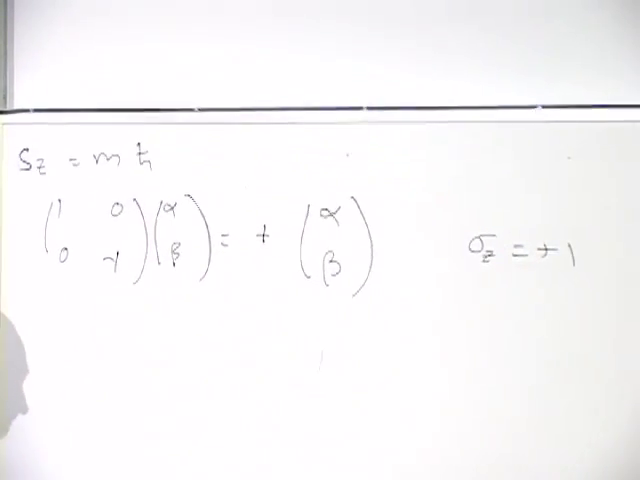
\includegraphics[width=0.74\textwidth]{lecture_08_figure_02.png}
\caption{معادلة القيمة الذاتية \(+1\) لـ \(\sigma_z\) عندما يؤثر في سبينور ذي مركبتين.}
\lectureframe{00:34:57}
\end{figure}

بالنسبة إلى القيمة الذاتية \(+1\)، فإن الضرب صفًا صفًا يعطي
\begin{equation}
\begin{pmatrix}
1\cdot\alpha+0\cdot\beta\\
0\cdot\alpha-\beta
\end{pmatrix}
=
\begin{pmatrix}
\alpha\\
-\beta
\end{pmatrix}
=
\begin{pmatrix}
\alpha\\
\beta
\end{pmatrix}.
\end{equation}
المعادلة العليا متحققة تلقائيًا، بينما تعطي السفلى \(-\beta=\beta\)، ومن ثم \(\beta=0\). ويشترط التطبيع \(|\alpha|=1\)؛ وباختيار الطور الكلي غير ذي الصلة بحيث \(\alpha=1\)،
\begin{equation}
|+z\rangle=
\begin{pmatrix}
1\\
0
\end{pmatrix}.
\end{equation}

بالنسبة إلى القيمة الذاتية \(-1\)،
\begin{equation}
\begin{pmatrix}
\alpha\\
-\beta
\end{pmatrix}
=
\begin{pmatrix}
-\alpha\\
-\beta
\end{pmatrix}.
\end{equation}
فالآن تكون المعادلة السفلى متحققة تلقائيًا، وتعطي العليا \(\alpha=-\alpha\)، ومن ثم \(\alpha=0\). وباختيار \(\beta=1\) نحصل على
\begin{equation}
|-z\rangle=
\begin{pmatrix}
0\\
1
\end{pmatrix}.
\end{equation}

الآن غيّر التجربة وقِس \(S_x\). وبما أن
\begin{equation}
\sigma_x
\begin{pmatrix}
\alpha\\
\beta
\end{pmatrix}
=
\begin{pmatrix}
0\cdot\alpha+\beta\\
\alpha+0\cdot\beta
\end{pmatrix}
=
\begin{pmatrix}
\beta\\
\alpha
\end{pmatrix},
\end{equation}
فإن معادلة \(+1\) تصبح
\begin{equation}
\begin{pmatrix}
\beta\\
\alpha
\end{pmatrix}
=
\begin{pmatrix}
\alpha\\
\beta
\end{pmatrix}.
\end{equation}
ومعادلتَا المركبتين، \(\beta=\alpha\) و\(\alpha=\beta\)، هما الشرط نفسه. ويعطي التطبيع
\begin{equation}
2|\alpha|^2=1,
\end{equation}
لذا فإن اختيارًا ملائمًا هو
\begin{equation}
|+x\rangle
=
\frac{1}{\sqrt2}
\begin{pmatrix}
1\\
1
\end{pmatrix}.
\end{equation}

\begin{figure}[t]
\centering
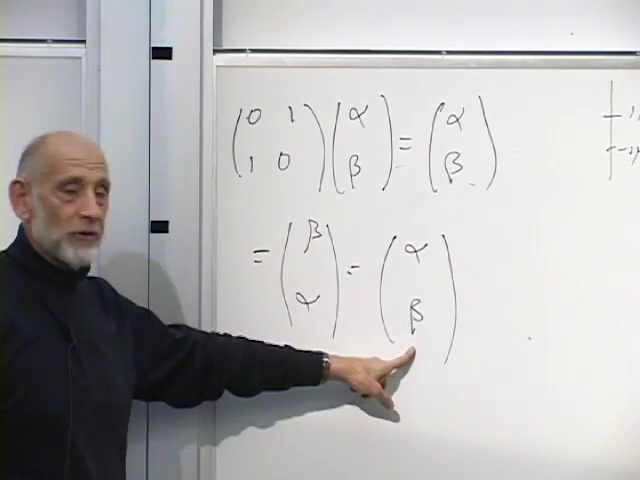
\includegraphics[width=0.74\textwidth]{lecture_08_figure_03.png}
\caption{بالنسبة إلى القيمة الذاتية \(+1\)، فإن \(\sigma_x\) يبدّل المركبتين، مما يقتضي \(\alpha=\beta\).}
\lectureframe{00:39:42}
\end{figure}

\begin{classroomqa}
\lecturetimestamp{00:40:13}
\audiencequestion{إذا أُدرج عامل النصف، فهل تكون القيمة الذاتية نصفًا؟}
\lecturerresponse{نعم. فمصفوفة باولي \(\sigma_x\) لها القيم الذاتية \(\pm1\)، بينما \(S_x=\sigma_x/2\) له القيم الذاتية \(\pm\tfrac12\).}
\end{classroomqa}

بالنسبة إلى القيمة الذاتية \(-1\)،
\begin{equation}
\begin{pmatrix}
\beta\\
\alpha
\end{pmatrix}
=
-
\begin{pmatrix}
\alpha\\
\beta
\end{pmatrix},
\end{equation}
إذًا
\begin{equation}
\beta=-\alpha,
\qquad
\alpha=-\beta.
\end{equation}
وهاتان هما، من جديد، المعادلة نفسها. وبعد التطبيع،
\begin{equation}
|-x\rangle
=
\frac{1}{\sqrt2}
\begin{pmatrix}
1\\
-1
\end{pmatrix}.
\end{equation}
وعليه فإن تراكبًا متساويًا من حالتي اللف المغزلي إلى أعلى على محور \(z\) وإلى أسفل على محور \(z\) يكون مستقطبًا على طول المحور \(x\) الموجب، بينما يكون التراكب نفسه مع إشارة سالبة نسبية مستقطبًا على طول المحور \(x\) السالب.

أما بالنسبة إلى اتجاه \(y\)،
\begin{equation}
\sigma_y
\begin{pmatrix}
\alpha\\
\beta
\end{pmatrix}
=
\begin{pmatrix}
-i\beta\\
i\alpha
\end{pmatrix}.
\end{equation}
فإن المتجهين الذاتيين المُطبَّعين هما
\begin{equation}
|+y\rangle
=
\frac{1}{\sqrt2}
\begin{pmatrix}
1\\
i
\end{pmatrix},
\qquad
|-y\rangle
=
\frac{1}{\sqrt2}
\begin{pmatrix}
1\\
-i
\end{pmatrix},
\end{equation}
وذلك حتى طور كلي. وتعطي كلتا الحالتين احتمالًا مقداره \(1/2\) لكون اللف المغزلي إلى أعلى على محور \(z\) و\(1/2\) لكونه إلى أسفل على محور \(z\). والطور النسبي \(i\)، الذي لا يظهر في هذين الاحتمالين، هو ما يميّز الاستقطاب على اتجاه \(y\) من الاستقطاب على اتجاه \(x\). كما تصف التركيبات الخطية أيضًا لفًا مغزليًا مستقطبًا على امتداد اتجاهات اعتباطية؛ ويُؤجَّل ذلك الحساب.

\begin{classroomqa}
\lecturetimestamp{00:44:22}
\audiencequestion{هل أُسنِدت إشارة مركبة \(i\) إلى القيمة الذاتية الخاطئة لـ \(\sigma_y\)؟}
\lecturerresponse{قد تكون الإشارة قد أُسنِدت فعلًا إلى القيمة الذاتية الخاطئة. والتعيين هنا غير مؤكد؛ ولا يُثبَّت هنا اعتمادًا على الذاكرة.}
\end{classroomqa}

والتحقق المباشر هو
\begin{align}
\sigma_y\frac{1}{\sqrt2}
\begin{pmatrix}
1\\
i
\end{pmatrix}
&=
\frac{1}{\sqrt2}
\begin{pmatrix}
-i\,i\\
i
\end{pmatrix}
=
\frac{1}{\sqrt2}
\begin{pmatrix}
1\\
i
\end{pmatrix},\\
\sigma_y\frac{1}{\sqrt2}
\begin{pmatrix}
1\\
-i
\end{pmatrix}
&=
\frac{1}{\sqrt2}
\begin{pmatrix}
(-i)(-i)\\
i
\end{pmatrix}
=
-\frac{1}{\sqrt2}
\begin{pmatrix}
1\\
-i
\end{pmatrix}.
\end{align}
ومن ثم فإن \(+i\) يقترن بالقيمة الذاتية \(+1\)، و\(-i\) يقترن بالقيمة الذاتية \(-1\).\footnote{يبقى التعيين الشفهي غير محسوم بعد عدة تبديلات؛ أما الإشارتان المعروضتان هنا فتتحددان بعملية ضرب المصفوفة المعروضة.} وكل حالة لف مغزلي نصفي، بما في ذلك كل حالة مستقطبة على امتداد اتجاه اعتباطي، هي تركيب خطي من \(|+z\rangle\) و\(|-z\rangle\).

\section{اللف المغزلي الواحد والسبينورات المعتمدة على الموضع}

بالنسبة إلى اللف المغزلي \(1\)، فإن القيم الممكنة لـ \(S_z\) هي \(+1,0,-1\). ومن ثم فإن فضاء الحالات ثلاثي الأبعاد. واللف المغزلي \(1\) لفٌّ صحيح ويقابل إحصاءً بوزونيًا. ونحن نبحث عن ثلاث مصفوفات \(3\times3\) تحقق مبدلات العزم الزاوي نفسها.

ويُعطى أدناه تمثيل متماثل بين الاتجاهات الإحداثية الثلاثة.\footnote{تتبع إشارة \(S_y\) المصفوفة الظاهرة قرب \(00{:}48{:}50\)، كما تتحدد أيضًا بواسطة \([S_x,S_y]=iS_z\). ومن شأن قلب تلك الإشارة أن يقلب المبدل المطلوب.}
\begin{equation}
\begin{aligned}
S_x
&=
i
\begin{pmatrix}
0&0&0\\
0&0&1\\
0&-1&0
\end{pmatrix},
&
S_y
&=
i
\begin{pmatrix}
0&0&1\\
0&0&0\\
-1&0&0
\end{pmatrix},\\
S_z
&=
i
\begin{pmatrix}
0&1&0\\
-1&0&0\\
0&0&0
\end{pmatrix}.
\end{aligned}
\end{equation}
كل مصفوفة هي \(i\) في مصفوفة حقيقية مضادة للتناظر. وتحتوي كل واحدة منها على مدخل مقداره \(1\) وآخر مقداره \(-1\)، وعلى صف وعمود منعدمَين مرتبطين بإحداثيها الخاص: الأول من أجل \(S_x\)، والثاني من أجل \(S_y\)، والثالث من أجل \(S_z\). وهذا يعطي أداة تذكّر مفيدة. وفي هذا التمثيل لا يكون \(S_z\) قطريًا.

لتكن
\begin{equation}
v=
\begin{pmatrix}
\alpha\\
\beta\\
\gamma
\end{pmatrix}.
\end{equation}
إذن
\begin{equation}
S_zv
=
\begin{pmatrix}
i\beta\\
-i\alpha\\
0
\end{pmatrix}.
\end{equation}
بالنسبة إلى القيمة الذاتية \(+1\)،
\begin{equation}
i\beta=\alpha,
\qquad
-i\alpha=\beta,
\qquad
0=\gamma.
\end{equation}
ومن ثم \(\beta=-i\alpha\) و\(\gamma=0\). ويعطي التطبيع \(2|\alpha|^2=1\)، لذا
\begin{equation}
|m=+1\rangle
=
\frac{1}{\sqrt2}
\begin{pmatrix}
1\\
-i\\
0
\end{pmatrix}.
\end{equation}
وبالنسبة إلى القيمة الذاتية \(-1\)،
\begin{equation}
i\beta=-\alpha,
\qquad
-i\alpha=-\beta,
\qquad
0=-\gamma,
\end{equation}
ومن ثم \(\beta=i\alpha\) و\(\gamma=0\)، و
\begin{equation}
|m=-1\rangle
=
\frac{1}{\sqrt2}
\begin{pmatrix}
1\\
i\\
0
\end{pmatrix}.
\end{equation}
وأخيرًا، تعطي معادلة القيمة الذاتية الصفرية \(\alpha=\beta=0\)، وتترك \(\gamma\) اعتباطيًا. وحلها المطبع هو
\begin{equation}
|m=0\rangle
=
\begin{pmatrix}
0\\
0\\
1
\end{pmatrix}.
\end{equation}
ولا توجد قيم ذاتية أخرى: فهذه المتجهات الذاتية الثلاثة تستنفد الفضاء الثلاثي الأبعاد. وليست العوامل \(1/\sqrt2\) شكلية فحسب. فالمعاملات نفسها تدخل لاحقًا في تنبؤات تجريبية كمية عندما يُطبَّق هذا الجبر على الإيزوسبين.

\begin{classroomqa}
\lecturetimestamp{00:54:10}
\audiencequestion{كيف ينبغي قراءة المدخلات العقدية لهذه المتجهات الذاتية للَّف المغزلي الواحد؟}
\lecturerresponse{بالنسبة إلى \(m=+1\) فالمركبات هي \(1/\sqrt2,-i/\sqrt2,0\)؛ وبالنسبة إلى \(m=-1\) فهي \(1/\sqrt2,i/\sqrt2,0\)؛ وبالنسبة إلى \(m=0\) فهي \(0,0,1\).}
\end{classroomqa}

توجد ثلاثيات أخرى من المصفوفات تحقق الجبر نفسه وهي مكافئة فيزيائيًا. والتمثيل المتماثل أعلاه مفيد لأنه يعامل الاتجاهات الثلاثة على السواء، وسيُستخدم مرة أخرى.

\subsection{استعادة الموضع}

والآن استعد حركة الجسيم. يتبادل اللف المغزلي مع الموضع ومع الزخم، لذا يمكن تحديد أيٍّ منهما معًا مع مركبة لف مغزلي. أما الموضع والزخم فلا يتبادلان، كما أن مركبات اللف المغزلي المختلفة لا تتبادل فيما بينها.

يُوصَف جسيم متحرك ذو لف مغزلي نصفي بسبينور يعتمد على الموضع،
\begin{equation}
\psi(x)=
\begin{pmatrix}
\psi_\uparrow(x)\\
\psi_\downarrow(x)
\end{pmatrix}.
\end{equation}
والكميتان
\begin{equation}
\rho_{\uparrow_z}(x)=|\psi_\uparrow(x)|^2,
\qquad
\rho_{\downarrow_z}(x)=|\psi_\downarrow(x)|^2
\end{equation}
هما كثافتا احتمال مشتركتان للموضع واللف المغزلي. ومجموعهما،
\begin{equation}
\rho(x)=\psi^\dagger(x)\psi(x)
=|\psi_\uparrow(x)|^2+|\psi_\downarrow(x)|^2,
\end{equation}
هو كثافة الموضع. وإذا كان معلومًا أن الجسيم قد كُشف عند \(x\)، فإن الاحتمالين الشرطيين هما
\begin{equation}
P(\uparrow_z\mid x)
=
\frac{|\psi_\uparrow(x)|^2}{\psi^\dagger(x)\psi(x)},
\qquad
P(\downarrow_z\mid x)
=
\frac{|\psi_\downarrow(x)|^2}{\psi^\dagger(x)\psi(x)},
\end{equation}
متى كان \(\rho(x)\neq0\). وهكذا يُمثَّل الإلكترون بدالة موجية مكانية ذات مركبتين، مع إمكان تغيّر سعات اللف المغزلي المحلية من موضع إلى آخر.

بالنسبة إلى جسيم متحرك ذي لف مغزلي واحد، نكتب
\begin{equation}
\phi(x)=
\begin{pmatrix}
\phi_1(x)\\
\phi_2(x)\\
\phi_3(x)
\end{pmatrix}.
\end{equation}
وعند كل نقطة في الفضاء، تُشكِّل المركبات الثلاث متجهًا في فضاء اللف المغزلي نفسه المستخدم أعلاه. وجسيمات اللف المغزلي الواحد لها لف مغزلي صحيح، وهي بوزونات.

\begin{classroomqa}
\lecturetimestamp{01:00:10}
\audiencequestion{هل تمثل \(\phi_1(x)\) نفسها احتمال النتيجة \(m=+1\) للَّف المغزلي؟}
\lecturerresponse{لا. إنها سعة في الأساس المختار ذي المركبات الثلاث. وللحصول على ناتج لف مغزلي محدد، كوِّن البرا للمتجه الذاتي المطبَّع الموافق، وأسقط الحقل عليه، ثم خذ مربع القيمة المطلقة.}
\end{classroomqa}

\begin{figure}[t]
\centering
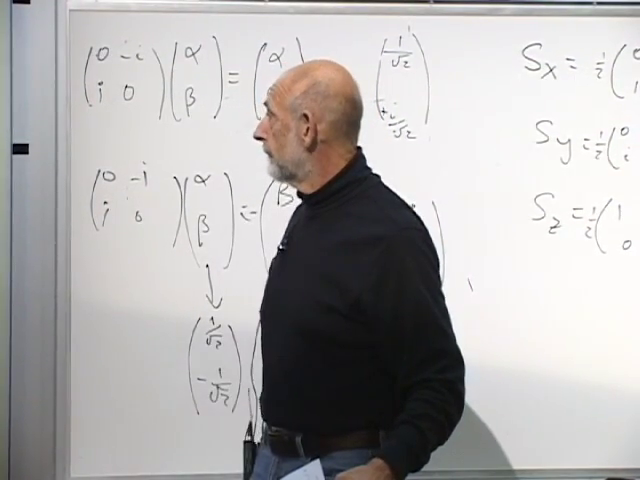
\includegraphics[width=0.82\textwidth]{lecture_08_figure_04.png}
\caption{المتجهات الذاتية المطبَّعة لـ \(\sigma_y\) إلى جانب المصفوفات الثلاث الخاصة باللف المغزلي نصف.}
\lectureframe{01:00:12}
\end{figure}

على سبيل المثال،
\begin{equation}
\begin{aligned}
|m=+1\rangle
&=
\frac{1}{\sqrt2}
\begin{pmatrix}
1\\
-i\\
0
\end{pmatrix}
\\
\Longrightarrow\quad\langle m=+1|
&=
\frac{1}{\sqrt2}
\begin{pmatrix}
1&i&0
\end{pmatrix}.
\end{aligned}
\end{equation}
ومن ثم فإن سعة الإسقاط هي
\begin{align}
\langle m=+1|\phi(x)\rangle
&=
\frac{1}{\sqrt2}
\begin{pmatrix}
1&i&0
\end{pmatrix}
\begin{pmatrix}
\phi_1(x)\\
\phi_2(x)\\
\phi_3(x)
\end{pmatrix}\\
&=
\frac{\phi_1(x)+i\phi_2(x)}{\sqrt2}.
\end{align}
ويعطي تطبيق القاعدة نفسها على المتجهات الذاتية الثلاثة كلها الكثافات المفصَّلة بحسب اللف المغزلي.\footnote{تُتم هذه الصيغ جبر الإسقاط بعد التصحيح الصريح بأن \(\phi_1\) و \(\phi_2\) ليسا بالضرورة حقيقيين. وإن معاملتهما على أنهما حقيقيان تمحو على نحو غير صحيح التداخل الذي يميز بين الكثافتين \(m=+1\) و \(m=-1\).}
\begin{align}
\rho_{+1}(x)
&=
\frac12\left|\phi_1(x)+i\phi_2(x)\right|^2,\\
\rho_{-1}(x)
&=
\frac12\left|\phi_1(x)-i\phi_2(x)\right|^2,\\
\rho_0(x)
&=
|\phi_3(x)|^2.
\end{align}
وهي تحقق
\begin{equation}
\begin{aligned}
\rho_{+1}(x)+\rho_{-1}(x)+\rho_0(x)
&=
|\phi_1(x)|^2+|\phi_2(x)|^2
\\
&\quad{}+|\phi_3(x)|^2
\\
&=
\phi^\dagger(x)\phi(x).
\end{aligned}
\end{equation}
وإذا اشترطنا أن الجسيم قد كُشف عند \(x\)، فإن
\begin{equation}
P(m\mid x)
=
\frac{\rho_m(x)}{\phi^\dagger(x)\phi(x)},
\end{equation}
بشرط \(\phi^\dagger(x)\phi(x)\neq0\). والقاعدة العامة للقياس هي دائمًا نفسها: كوِّن البرا للمتجه الذاتي المطبَّع المطلوب، وأسقط الحالة الفعلية عليه، ثم خذ مربع القيمة المطلقة. وتحتفظ الكثافة الناتجة باعتمادها على الموضع.

مصفوفات اللف الأعلى أكثر تعقيدًا، لكن المبدأ لا يتغير.

\begin{classroomqa}
\lecturetimestamp{01:07:31}
\audiencequestion{ما بُعد فضاء الحالات للَّف المغزلي ثلاثة أنصاف؟}
\lecturerresponse{له أربع حالات، مع \(m=\tfrac32,\tfrac12,-\tfrac12,-\tfrac32\). أما اللف المغزلي اثنان فله خمس حالات.}
\end{classroomqa}

\begin{classroomqa}
\lecturetimestamp{01:07:55}
\audiencequestion{لماذا اشتملت المناقشة على \(x,y,z\) من دون اتجاه زمني؟ أهذه المعالجة لا نسبوية؟}
\lecturerresponse{حتى الآن هي معالجة لا نسبوية. فاللف المغزلي، مثل الكتلة، يُميَّز بأبسط صورة في إطار سكون الجسيم؛ ويُستحصل على وصفه في إطار عطالي آخر بتحويل لورنتز المناسب. وتُؤجَّل تلك الخطوة النسبوية.}
\end{classroomqa}

توفر معادلة ديراك الإطار النسبي وتفسر لماذا تحتوي دالتها الموجية ذات المركبات الأربع على ازدواج لف مغزلي.

\section{مصفوفات ديراك والسبينور ذو المركبات الأربع}

تحقق الدالة الموجية الديراكية ذات المركبات الأربع
\begin{equation}
i\frac{\partial\Psi}{\partial t}
=
-i\alpha_i\frac{\partial\Psi}{\partial x_i}
+m\beta\Psi,
\qquad i=1,2,3,
\end{equation}
حيث يُجمَع على أي فهرس مكاني مكرر. ومن ثم فإن حد المشتقة يعني
\begin{equation}
\alpha_1\frac{\partial\Psi}{\partial x}
+\alpha_2\frac{\partial\Psi}{\partial y}
+\alpha_3\frac{\partial\Psi}{\partial z}.
\end{equation}
وبالنسبة إلى موجة مستوية، تصبح هذه المعادلة الجبرية
\begin{equation}
\omega\Psi=(\alpha_i k_i+m\beta)\Psi.
\end{equation}

\begin{classroomqa}
\lecturetimestamp{01:11:32}
\audiencequestion{هل تدل المرتان اللتان يَرِد فيهما \(m\) على الشيء نفسه؟}
\lecturerresponse{لا. استُخدمت إحداهما بوصفها فهرسًا مكانيًا، والأخرى هي كتلة الجسيم. أعد تسمية الفهرس المكاني \(i\)؛ وعندما يَرِد \(i\) مرتين يُجمَع من \(1\) إلى \(3\).}
\end{classroomqa}

إن تربيع مؤثر التردد يجب أن يعيد إنتاج العلاقة النسبية
\begin{equation}
\omega^2=\mathbf{k}^2+m^2.
\end{equation}
ولذلك تقتضي الحدود التربيعية، لكل \(i\)،
\begin{equation}
\alpha_i^2=I_4,
\qquad
\beta^2=I_4.
\end{equation}

\begin{classroomqa}
\lecturetimestamp{01:13:01}
\audiencequestion{هل يختلف \(\beta\) باختلاف كل واحدة من المركبات الأربع لـ \(\Psi\)؟}
\lecturerresponse{لا. توجد مصفوفة واحدة هي \(\beta\)، وهي تؤثر في السبينور كله ذي المركبات الأربع، وتحقق \(\beta^2=I_4\).}
\end{classroomqa}

يجب أن تنعدم الحدود المختلطة. وبالنسبة إلى الاتجاهات المكانية المختلفة، وكذلك بين كل \(\alpha_i\) و \(\beta\)، نحصل على
\begin{equation}
\alpha_i\alpha_j+\alpha_j\alpha_i=0
\quad (i\neq j),
\qquad
\alpha_i\beta+\beta\alpha_i=0.
\end{equation}
وبصورة مكافئة،
\begin{equation}
\{\alpha_i,\alpha_j\}=2\delta_{ij}I_4,
\quad
\{\alpha_i,\beta\}=0,
\quad
\{\beta,\beta\}=2I_4.
\end{equation}
كل مصفوفة تتضاد تبادليًا مع كل مصفوفة مختلفة عنها، في حين أن مضاد المبدلة لها مع نفسها يساوي ضعفي مصفوفة الوحدة.

لولا \(\beta\)، لكانت مصفوفات باولي الثلاث توفر بالفعل ثلاث مصفوفات \(2\times2\) مربعاتها تساوي الهوية وتتضاد تبادليًا زوجيًا. ويتطلب حد الكتلة مصفوفة رابعة من هذا النوع. ولا توجد مصفوفة رابعة \(2\times2\) بالخواص المطلوبة، كما أن مصفوفات \(3\times3\) لا تحقق هذا الجبر أيضًا. ولذلك فإن أصغر تمثيل هو \(4\times4\).

يمكن تقسيم مصفوفة \(4\times4\) إلى أربع كتل \(2\times2\). وفي أحد التمثيلات الملائمة،
\begin{equation}
\alpha_i=
\begin{pmatrix}
\sigma_i&0\\
0&-\sigma_i
\end{pmatrix},
\qquad i=1,2,3.
\end{equation}

\begin{figure}[t]
\centering
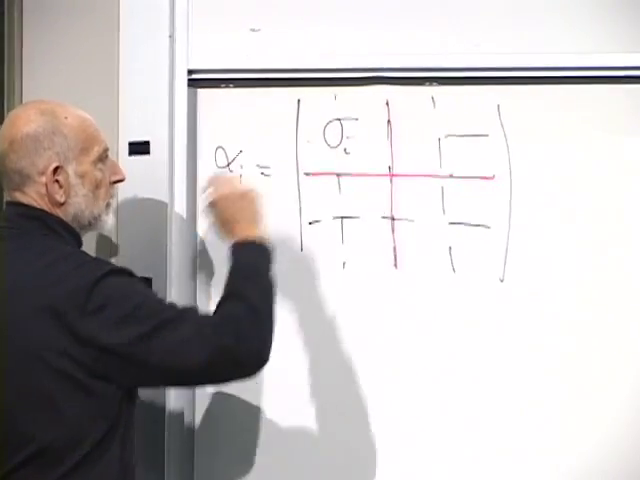
\includegraphics[width=0.68\textwidth]{lecture_08_figure_05.png}
\caption{مصفوفة ديراك \(\alpha_i\) مكتوبة على هيئة كتل \(2\times2\)، مع \(\sigma_i\) و \(-\sigma_i\) على القطر.}
\lectureframe{01:17:23}
\end{figure}

\begin{classroomqa}
\lecturetimestamp{01:17:41}
\audiencequestion{هل كانت كتل \(\sigma_i\) مرتبة على النحو المعاكس في التمثيل السابق؟}
\lecturerresponse{نعم. فقد وُضعت خارج القطر في تمثيل آخر. والترتيبان متكافئان، ويرتبط أحدهما بالآخر بتحويل تشابه.}
\end{classroomqa}

في التمثيل الحالي تكون المصفوفة المتبقية هي
\begin{equation}
\beta=
\begin{pmatrix}
0&I_2\\
I_2&0
\end{pmatrix},
\qquad
I_2=
\begin{pmatrix}
1&0\\
0&1
\end{pmatrix}.
\end{equation}
ويختزل ضرب الكتل التحقق من جبر \(4\times4\) إلى ضرب اعتيادي لمصفوفات \(2\times2\).

\begin{classroomqa}
\lecturetimestamp{01:19:17}
\audiencequestion{هل استخدم التمثيل السابق إشارة مختلفة أو شكلًا قطريًا لـ \(\beta\)؟}
\lecturerresponse{لقد استخدم أساسًا مختلفًا لكنه مكافئ فيزيائيًا. ويخلط تغيير الأساس المركبات الأربع لـ \(\Psi\) ويغيّر مظهر المصفوفات من غير أن يغيّر الفيزياء.}
\end{classroomqa}

المركبات الأربع لـ \(\Psi\) ليست هي الإحداثيات الأربع للزمكان. بل هي إحداثيات في أصغر فضاء متجهي يمكن أن يؤثر عليه جبر مضادات التبديل هذا. وهناك بنيتان ثنائيتان متميزتان: التقسيم إلى كتل \(2\times2\)، والبنية الباولية ثنائية المركبة داخل كل كتلة. واستباقًا للتفسير الذي سيثبت أدناه، يمكن تنظيم الإمكانات الأربع على الصورة
\begin{equation}
\begin{array}{c|cc}
& S_z=+\tfrac12 & S_z=-\tfrac12\\ \hline
\omega>0 & (\omega>0,+\tfrac12) & (\omega>0,-\tfrac12)\\
\omega<0 & (\omega<0,+\tfrac12) & (\omega<0,-\tfrac12)
\end{array}.
\end{equation}
ويتألف الصف السفلي من حالات إلكترون ذات تردد سالب. وهو ليس صفًا من البوزيترونات؛ فسيُفسَّر البوزيترون على أنه ثقب في المجموعة الممتلئة من تلك الحالات.

\section{تضاعف الطاقة في إطار السكون والبوزيترون}

أسهل ما يكون إظهار البنية الثنائية للطاقة عند انعدام الزخم. فعندما يكون \(\mathbf{k}=0\)، تكون حالة الموجة المستوية ثابتة مكانيًا ويختفي حد المشتقة المكانية. ومعادلة إطار السكون\footnote{تحتفظ الشريحة عند \(01{:}23{:}38\) مؤقتًا بعامل إضافي هو \(i\) في حد الكتلة؛ ويزيله التصحيح المنطوق عند \(01{:}24{:}05\).} هي
\begin{equation}
i\frac{\partial\Psi}{\partial t}=m\beta\Psi.
\end{equation}

\begin{figure}[t]
\centering
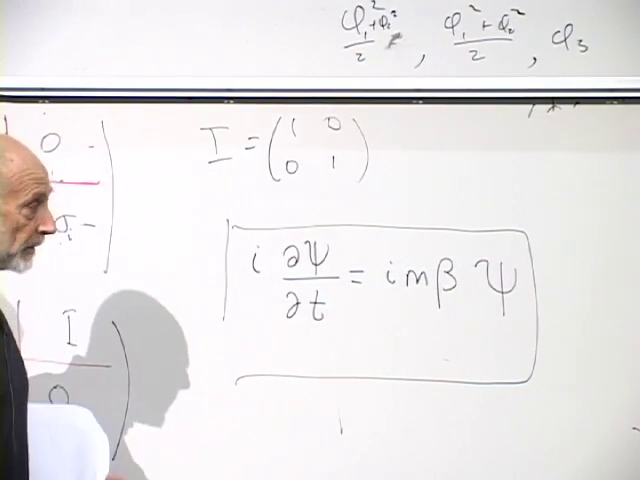
\includegraphics[width=0.76\textwidth]{lecture_08_figure_06.png}
\caption{عند انعدام الزخم تنعدم المشتقات المكانية، فتبقى معادلة إطار السكون المصححة \(i\partial_t\Psi=m\beta\Psi\).}
\lectureframe{01:23:38}
\end{figure}

قسّم العمود ذا المركبات الأربع إلى جزأين، علوي وسفلي، لكل منهما مركبتان:
\begin{equation}
\Psi=
\begin{pmatrix}
\psi_+\\
\psi_-
\end{pmatrix}.
\end{equation}

\begin{classroomqa}
\lecturetimestamp{01:24:47}
\audiencequestion{هل تعني التسميتان \(\psi_+\) و \(\psi_-\) بالفعل الطاقة الموجبة والطاقة السالبة؟}
\lecturerresponse{لا. ففي هذه المرحلة هما مجرد اسمين للكتلتين العلوية والسفلية ثنائيتَي المركبات. ولم تُستخرج تراكيبهما الطاقية بعد.}
\end{classroomqa}

\begin{classroomqa}
\lecturetimestamp{01:25:10}
\audiencequestion{ماذا يمثل العمود المقسَّم ذو المركبات الأربع؟}
\lecturerresponse{إنه السبينور الديراكي نفسه ذو المركبات الأربع، منظَّمًا بحيث يطابق صيغة الكتل للمصفوفات. وكل نصف هو عنصر ذو مركبتين، وعنصران كهذان يكوِّنان العمود الأصلي ذا المركبات الأربع.}
\end{classroomqa}

تبدّل المصفوفة \(\beta\) الكتلتين:
\begin{equation}
\beta
\begin{pmatrix}
\psi_+\\
\psi_-
\end{pmatrix}
=
\begin{pmatrix}
\psi_-\\
\psi_+
\end{pmatrix}.
\end{equation}
ولذلك تصبح معادلة إطار السكون
\begin{equation}
i\frac{\partial\psi_+}{\partial t}=m\psi_-,
\qquad
i\frac{\partial\psi_-}{\partial t}=m\psi_+.
\end{equation}

هناك اقتراحان طبيعيان. فأخذ مشتقة زمنية أخرى من شأنه أن يفصل النظام، لكن جمع المعادلتين وطرحهما يجعلهما في صورة قطرية فورًا. وفي الواقع،
\begin{align}
i\frac{\partial}{\partial t}(\psi_++\psi_-)
&=m(\psi_++\psi_-),\\
i\frac{\partial}{\partial t}(\psi_+-\psi_-)
&=-m(\psi_+-\psi_-).
\end{align}
وبتعريف
\begin{equation}
\chi_+=\psi_++\psi_-,
\qquad
\chi_-=\psi_+-\psi_-,
\end{equation}
نحصل على معادلتين مستقلتين،
\begin{equation}
i\partial_t\chi_+=m\chi_+,
\qquad
i\partial_t\chi_-=-m\chi_-.
\end{equation}
وبالنسبة إلى اعتماد ذي تردد محدد \(e^{-i\omega t}\)، يكون للمجموع
\begin{equation}
\omega=+m,
\end{equation}
بينما يكون للفرق
\begin{equation}
\omega=-m.
\end{equation}
وهذا هو بالضبط تضاعف الطاقة الموجبة والسالبة الذي وُجد في المثال الأحادي البعد السابق: فالمعادلة النسبية تمتلك مرة أخرى حلول إلكترون ذات طاقة موجبة وحلول إلكترون ذات طاقة سالبة. ومن ثم ينفصل تضاعف الكتل إلى فرعين للطاقة الموجبة والسالبة. ويمكن كتابة حالات إطار السكون الخالصة على الصورة
\begin{equation}
\Psi_{\omega=+m}=
\begin{pmatrix}
\xi\\
\xi
\end{pmatrix},
\qquad
\Psi_{\omega=-m}=
\begin{pmatrix}
\xi\\
-\xi
\end{pmatrix},
\end{equation}
حيث تظل \(\xi\) عنصرًا اعتباطيًا ذا مركبتين.

لقد تخلَّص المجموع والفرق من إحدى البنيتين الثنائيتين، لكن المركبتين في \(\xi\) تبقيان. وتؤثر مصفوفات باولي في هذا الزوج المتبقي. وهذا هو الزوج المرتبط باللف المغزلي، والخاضع للتحقق المتعلق بالدوران وقانون الانحفاظ الذي سيُناقش أدناه.

\begin{classroomqa}
\lecturetimestamp{01:32:23}
\audiencequestion{هل يمكن التعامل مع اللف المغزلي بوصفه البنية الثنائية الخارجية، ومع إشارة الطاقة بوصفها الداخلية؟}
\lecturerresponse{نعم. إن ترتيبي العاملين متكافئان. ويمكن تبديل أي الفهرسين يُكتب أولًا؛ فالتغيير ليس إلا إعادة ترتيب للمركبات الأربع.}
\end{classroomqa}

يقود فرع التردد السالب إلى تفسير بحر ديراك. ويُسنَد إلى التردد السالب طاقة إلكترون سالبة. وملء كل حالة إلكترون سالبة الطاقة يخفِّض الطاقة إلى أبعد مدى يسمح به مبدأ الاستبعاد، لأن إلكترونًا واحدًا فقط يمكنه أن يشغل كل حالة فيرميونية كاملة. وعندئذ يُسمَّى بحر الطاقة السالبة الممتلئ تمامًا الفراغ.

انقل إلكترونًا واحدًا من هذا البحر المملوء إلى حالة موجبة الطاقة. تحتوي النتيجة على إلكترون ذي طاقة موجبة وعلى حالة سالبة الطاقة غير مشغولة. إن إزالة طاقة سالبة ترفع الطاقة، لذا تكون للفجوة طاقة إثارة موجبة؛ ولأن إلكترونًا مفقود، فإنها تحمل أيضًا الشحنة الكهربائية المعاكسة. الفجوة هي بوزيترون.

\begin{classroomqa}
\lecturetimestamp{01:32:57}
\audiencequestion{هل يمكن شرح تفسير البوزيترون مرة أخرى؟}
\lecturerresponse{مجموع الجزأين له تردد موجب وفرقُهما له تردد سالب. وحلول التردد السالب هي حالات إلكترون سالبة الطاقة، ويُحصَل على الفراغ بملء جميعها. إن رفع أحد الإلكترونات المشغولة إلى طاقة موجبة يترك إلكترونًا ذا طاقة موجبة وفجوةً معًا. وتلك الفجوة ذات الطاقة الموجبة والشحنة المعاكسة هي البوزيترون.}
\end{classroomqa}

وهكذا أنتج الجبر في آن واحد نتيجتين: فرعي الطاقة الموجبة والسالبة، اللذين يصبحان بنية الجسيم--ضد الجسيم، وبنيةً متبقيةً ذات مركبتين مرتبطة بلف مغزلي مقداره نصف. والنقطة اللافتة هي أن كليهما انبثق من أصغر المصفوفات القادرة على استيفاء علاقات ضديد التبديل النسبية. ولم يكن اللف المغزلي قد ظهر إلا حديثًا بوصفه خاصية تجريبية حين أنتج هذا البناء الرياضي جسيماتٍ ذات لف مغزلي مع فرعٍ لضد الجسيم؛ وفي ذلك السياق التاريخي كانت النتيجة مثيرة.

\begin{classroomqa}
\lecturetimestamp{01:35:14}
\audiencequestion{هل الإلكترونات سالبة الطاقة نفسها هي البوزيترونات؟}
\lecturerresponse{لا. حالات الإلكترون سالبة الطاقة مملوءة في الفراغ. والبوزيترون هو غياب إلكترون واحد من تلك المجموعة المملوءة: فجوة، لا إلكترون سالب الطاقة.}
\end{classroomqa}

يمكن للفجوة أن تشارك في انتقالات. وللبوزيترون طاقة موجبة لأنه غياب إلكترون سالب الطاقة. وإذا ملأ إلكترون ذو طاقة موجبة الفجوة، فإن الإلكترون والبوزيترون يفني أحدهما الآخر، ولكن لا بد أن تُحمَل طاقتهما بعيدًا، عادةً بواسطة الفوتونات. وبلغة البحر، يكون إلكترون قد ملأ حالة سالبة الطاقة غير مشغولة. ويمكن تصوير انطلاق الطاقة نفسه كما لو أن إلكترونًا مثارًا في ذرة يهبط إلى مستوى أدنى: فالانتقال الهابط يبعث فوتونات.

\begin{classroomqa}
\lecturetimestamp{01:36:39}
\audiencequestion{لماذا لا تهبط الإلكترونات الواقعة عند طاقات سالبة أعلى إلى الفجوة؟}
\lecturerresponse{هذا السؤال يخلط بين حالتين. فملء الفجوة بإلكترون ذي طاقة موجبة هو إفناء إلكترون--بوزيترون، مع حمل الفوتونات للطاقة بعيدًا. أما انتقال إلكترون من بحر الطاقات السالبة فهو عملية مختلفة، ستُتناول أدناه.}
\end{classroomqa}

إن حساب الزخم الصفري، بمفرده، قد أثبت انحلالًا ثنائيًا بعد فصل إشارة الطاقة. لكن وجود انحلال بين حالتين ليس، بمفرده، برهانًا على أن هاتين الحالتين تحملان زخمًا زاويًا.

\begin{classroomqa}
\lecturetimestamp{01:37:44}
\audiencequestion{كيف يثبت حساب الزخم الصفري أن الزوج المتبقي من الحالات يمثل لفًا مغزليًا؟}
\lecturerresponse{يمكن تسمية هذا الزوج أعلى وأسفل، وتظهر مصفوفات باولي في المعادلة الكاملة، لكن ذلك وحده ليس برهانًا بعد. فلا بد إما من إظهار كيف يتحول الزوج تحت الدورانات المكانية، أو من أن إسناد لف مغزلي إليه يجعل الزخم الزاوي الكلي محفوظًا في التفاعلات والتصادمات. ويُؤجَّل هذا البرهان.}
\end{classroomqa}

بالنسبة إلى حالة سكون موجبة الطاقة، يكون الجزآن العلوي والسفلي متساويين،
\begin{equation}
\Psi_{\omega=+m}=
\begin{pmatrix}
\xi\\
\xi
\end{pmatrix}.
\end{equation}
وأما إثبات أن \(\xi\) يشكل مزدوجة زخم زاوي، فيتطلب حجة الدوران أو الانحفاظ التي وُصفت للتو؛ ولا يترتب ذلك لمجرد عد مركبتين.

\begin{classroomqa}
\lecturetimestamp{01:40:46}
\audiencequestion{هل يمكن لإلكترون مختلف أن يفنى مع البوزيترون حتى لو كانت طاقته مختلفة؟}
\lecturerresponse{نعم. لا تحتفظ الإلكترونات بأي هوية فردية. ويمكن لأي إلكترون متاح أن يملأ الفجوة، وتنعكس الفروق في الطاقة والزخم الابتدائيين في عدد الفوتونات المنبعثة وطاقاتها.}
\end{classroomqa}

كما تفسر صورة الفجوة أيضًا انتقالًا يقع بأكمله داخل بحر الطاقات السالبة. افترض أن حالة سالبة الطاقة مشغولة انتقلت إلى الفجوة. عندئذٍ تُملأ الفجوة الأصلية، لكن الحالة التي جاء منها ذلك الإلكترون تصبح الآن فارغة. لقد انتقلت الفجوة. وبصورة مكافئة، يكون البوزيترون قد غيّر طاقته وأصدر إشعاعًا.

\begin{classroomqa}
\lecturetimestamp{01:42:12}
\audiencequestion{لماذا لا يمكن للمستويات سالبة الطاقة المجاورة أن تهبط تباعًا إلى الفجوة؟}
\lecturerresponse{يمكنها أن تنقل الفجوة من مستوى إلى آخر. فإلكترون يهبط إلى الفجوة القديمة يترك فجوة جديدة عند طاقته السابقة، ولذلك يصبح البوزيترون الابتدائي بوزيترونًا ذا طاقة مختلفة. وتحمل الفوتونات فرق الطاقة.}
\end{classroomqa}

\begin{classroomqa}
\lecturetimestamp{01:44:39}
\audiencequestion{لماذا لا يؤدي هذا إلى شلالٍ إشعاعي هابط بلا نهاية؟}
\lecturerresponse{لأن الطاقة والزخم يجب أن يُحفَظا في آن واحد. وهذان قانونا الانحفاظ لا يسمحان بهذه العملية غير المقيّدة. وتنشأ المسألة نفسها بالنسبة إلى إلكترون حر عادي: إذ لا يمكنه ببساطة أن يواصل خفض طاقته بإصدار فوتونات في الفضاء الخالي.}
\end{classroomqa}
\chapter{اللاجرانجيات والحقول وعمليات الجسيمات المحلية}

حقول البوزونات وحقول الفرميونات والحقل الكهرومغناطيسي كلها تخضع لمعادلات ذات طابع موجي. وتتضمن تلك المعادلات الحقول نفسها إلى جانب مشتقاتها المكانية والزمانية. ويمكن للمرء أن يسرد معادلة حركة منفصلة لكل حقل، لكن اللاجرانجي يجمع المنظومة بأكملها في تعبير مدمج واحد. ويعطي تطبيق قاعدة أويلر--لاجرانج على ذلك التعبير معادلات جميع الحقول دفعة واحدة.

هذا البناء يرتبط ارتباطًا وثيقًا بالفعل الساكن. والمهمة المباشرة هنا أكثر تحديدًا: تحديد ما الذي يعتمد عليه لاجرانجي الحقل، واستخدامه لاستخراج بضع معادلات كلاسيكية، ثم إعادة تفسير تعابير الحقول نفسها تفسيرًا كموميًا. وفي النظرية الكمومية يحكم اللاجرانجي حركة الجسيمات وتآثرها، وفي نهاية المطاف سعات التصادمات ومقاطعها العرضية.

\section{ترميز مدمج لمعادلات الحقول}

لحقل قياسي واحد، تعتمد الكثافة اللاجرانجية على الحقل وعلى مشتقاته الأولى،
\begin{equation}
\mathcal L
=
\mathcal L\!\left(\phi,\partial_t\phi,\partial_x\phi,\ldots\right)
=
\mathcal L\!\left(\phi,\partial_\mu\phi\right).
\end{equation}
وغالبًا ما تكون القائمة الصريحة للمشتقات الزمانية والمكانية أكثر فائدة أثناء الحساب؛ أمّا الترميز \(\partial_\mu\phi\) فيجمع القائمة نفسها في صيغة نسبية.

\begin{figure}[htbp]
\centering
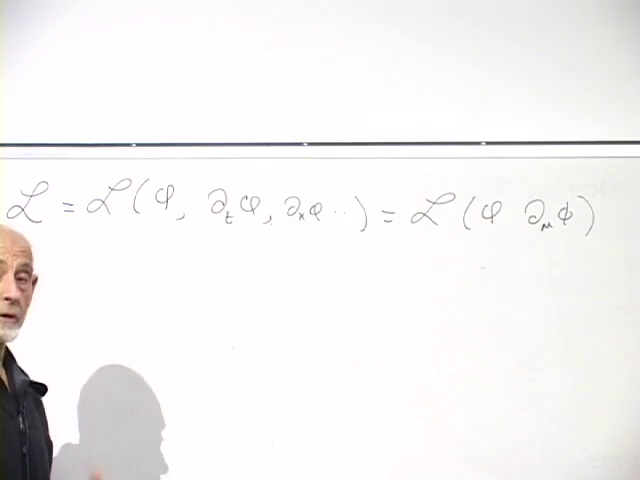
\includegraphics[width=0.82\textwidth]{lecture_09_figure_03.png}
\caption{اعتماد لاجرانجي لحقل قياسي على الحقل وعلى مشتقاته الزمكانية.}
\lectureframe{00:03:56}
\end{figure}

ومعادلة أويلر--لاجرانج للحقل هي
\begin{equation}
\frac{\partial}{\partial t}
\frac{\partial\mathcal L}{\partial\dot\phi}
+
\frac{\partial}{\partial x}
\frac{\partial\mathcal L}{\partial\phi_x}
+
\frac{\partial}{\partial y}
\frac{\partial\mathcal L}{\partial\phi_y}
+
\frac{\partial}{\partial z}
\frac{\partial\mathcal L}{\partial\phi_z}
=
\frac{\partial\mathcal L}{\partial\phi},
\end{equation}
حيث
\begin{equation}
\dot\phi=\frac{\partial\phi}{\partial t},
\qquad
\phi_x=\frac{\partial\phi}{\partial x},
\qquad
\phi_y=\frac{\partial\phi}{\partial y},
\qquad
\phi_z=\frac{\partial\phi}{\partial z}.
\end{equation}
وإذا كانت \(\mathcal L\) تتضمن عدة حقول، فتُطبَّق هذه القاعدة مرة واحدة على كل حقل. والنتيجة هي منظومة معادلات الحركة.

وأبسط مثال لحقل قياسي هو
\begin{equation}
\begin{split}
\mathcal L
&=
\frac12\dot\phi^2
-\frac12\phi_x^2
-\frac12\phi_y^2
-\frac12\phi_z^2
-V(\phi)
\\
&=
\frac12\dot\phi^2-\frac12(\boldsymbol\nabla\phi)^2-V(\phi).
\end{split}
\end{equation}
وتحمل حدود المشتقات المكانية إشارة معاكسة لإشارة حد المشتقة الزمنية. وبالتفاضل حدًا حدًا نحصل على
\begin{align}
\frac{\partial\mathcal L}{\partial\dot\phi}&=\dot\phi,
&
\frac{\partial\mathcal L}{\partial\phi_i}&=-\phi_i,
&
\frac{\partial\mathcal L}{\partial\phi}&=-V'(\phi),
\end{align}
ولذلك
\begin{equation}
\ddot\phi-\nabla^2\phi=-V'(\phi).
\end{equation}

\begin{figure}[htbp]
\centering
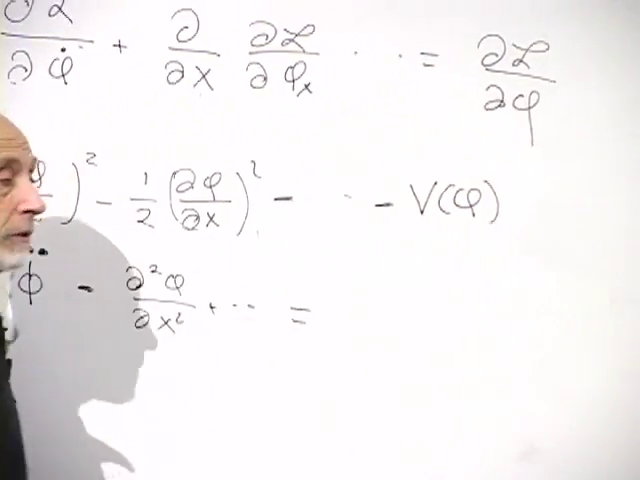
\includegraphics[width=0.74\textwidth]{lecture_09_figure_04.png}
\caption{معادلة أويلر--لاجرانج، ولاجرانجي الحقل القياسي، ومعادلة الحقل التي يولدها \(V(\phi)\).}
\lectureframe{00:08:23}
\end{figure}

هذه هي المعادلة التي يولدها لاجرانجي الحقل القياسي.\editorialnote{الإطار المحتفَظ به مقصوص عند الحافة اليسرى؛ والإكمال المعروض يحدده الاشتقاق الشفهي المحيط به مباشرة.}

هنا \(V(\phi)\) هي كثافة طاقة الوضع للحقل. وليس لمساهمة ثابتة في \(V\) أي أثر في هذه المعادلة لأن مشتقتها تنعدم. وجهد خطي ممكن جبريًا، لكنه لا يملك حدًا أدنى: إذ يمكن لطاقة الحقل أن تنحدر نحو سالب ما لا نهاية. لذلك فإن أول مثال مستقر هو
\begin{equation}
V(\phi)=\frac12m^2\phi^2,
\qquad
V'(\phi)=m^2\phi,
\end{equation}
الذي يعطي
\begin{equation}
\ddot\phi-\nabla^2\phi=-m^2\phi.
\end{equation}

ولإبراز معنى \(m\)، نعوّض بموجة مستوية،
\begin{equation}
\phi(\mathbf x,t)=\phi_0e^{i\omega t-i\mathbf k\cdot\mathbf x}.
\end{equation}
وعندئذ
\begin{equation}
\ddot\phi=-\omega^2\phi,
\qquad
\nabla^2\phi=-\mathbf k^2\phi,
\end{equation}
فتصبح معادلة الموجة
\begin{equation}
-\omega^2\phi+\mathbf k^2\phi=-m^2\phi.
\end{equation}
وبعد اختزال \(\phi\)،
\begin{equation}
\omega^2=\mathbf k^2+m^2.
\end{equation}
وفي وحدات يكون فيها \(\hbar=c=1\)، يكون التردد طاقة ويكون العدد الموجي زخمًا. ومن ثم
\begin{equation}
E^2=\mathbf p^2+m^2,
\end{equation}
أو، بعد إعادة قوى \(c\)، \(E^2=\mathbf p^2c^2+m^2c^4\). والمعلمة \(m\) هي كتلة كمّ واحد من الحقل.

يمكن فرض الثبات النسبي على مستوى الصياغة الموجزة. فإذا كانت \(\mathcal L\) كميةً قياسية لورنتزية، كانت معادلات حركتها ثابتةً تحت تحولات لورنتز. والإشارة النسبية بين المشتقات الزمنية والمكانية هي إشارة الزمكان المألوفة في النسبية الخاصة.

\section{اللاخطية والحقول الكلاسيكية المقترنة}

تُدخل الأسس الأعلى للحقل نوعًا جديدًا من السلوك. فإذا كان
\begin{equation}
V(\phi)=\frac12m^2\phi^2+g\phi^3,
\end{equation}
فإن
\begin{equation}
\ddot\phi-\nabla^2\phi=-m^2\phi-3g\phi^2.
\end{equation}
تعطي الحدود التربيعية في اللاغرانجي معادلات خطية في الحقل. أما الحدود التكعيبية وما فوقها فتعطي معادلات لاخطية.

يظهر هذا التمييز في حركة الحزم الموجية. ففي معادلة خطية، يمكن جمع حزمة متحركة نحو اليمين وحزمة متحركة نحو اليسار لتكوين حل آخر. وهما تتراكبان وتتداخلان مدةً من الزمن، ثم تمر كل منهما خلال الأخرى وتخرجان بأشكالهما الأصلية. أما مع الحدود اللاخطية، فتؤثر الحزم بعضها في بعض. ويمكنها أن تتشتت، أو تتشوه، أو تتفكك إلى موجات أشد تعقيدًا. والتداخل المؤقت للموجات الخطية ليس تفاعلًا؛ أما التغير الدائم في الحزم فيدل على اللاخطية.

يظهر النمط نفسه مع حقلين قياسيين. لنأخذ
\begin{align}
\mathcal L
&=
\frac12(\partial_\mu\phi)(\partial^\mu\phi)
+\frac12(\partial_\mu\rho)(\partial^\mu\rho)
-V(\phi,\rho),
\\
V(\phi,\rho)
&=
\frac12m^2\phi^2+\frac12M^2\rho^2+\rho\phi^2.
\end{align}
ومن دون الحد الأخير تكون المعادلتان مستقلتين،
\begin{equation}
\ddot\phi-\nabla^2\phi=-m^2\phi,
\qquad
\ddot\rho-\nabla^2\rho=-M^2\rho.
\end{equation}
وهما تصفان كمّات من نوعين، كتلتهما \(m\) و\(M\). ومع إدراج الحد المختلط،
\begin{align}
\ddot\phi-\nabla^2\phi&=-m^2\phi-2\rho\phi,
\\
\ddot\rho-\nabla^2\rho&=-M^2\rho-\phi^2.
\end{align}
تحتوي كل معادلة الآن على الحقل الآخر. فالمعادلتان مقترنتان ولاخطيّتان: إذ تبعثر حزمة \(\phi\) حزمة \(\rho\)، والعكس بالعكس. وتحكم حدود المشتقات علاقة الطاقة--الزخم، وتحدد الحدود التربيعية غير المشتقة الكتل، ويحمل الحد المختلط الأعلى رتبةً التفاعل. وهذا هو النمط الكلاسيكي الأساسي.

\section{حقول ديراك واقتران قياسي}

بالنسبة إلى حقل ديراك، تكون المعادلة من الرتبة الأولى في الزمن. وفي اختزال أحادي البعد، مع فهم الامتداد إلى ثلاثة اتجاهات مكانية، تكون بنية حدوده كما يلي
\begin{equation}
i\dot\Psi
\simeq
i\alpha\frac{\partial\Psi}{\partial x}+m\beta\Psi,
\qquad
i\boldsymbol\alpha\cdot\boldsymbol\nabla\Psi
=i\sum_i\alpha_i\frac{\partial\Psi}{\partial x_i}.
\end{equation}
وتؤثر المصفوفات \(\alpha_i\) و\(\beta\) في مركبات \(\Psi\). ويحتوي لاغرانجي مناظر على حد خطي في \(\partial_t\Psi\)، وحد ثنائي خطي في المشتقة المكانية يتضمن \(\alpha_i\)، وحد الكتلة الثنائي الخطي \(m\Psi^\dagger\beta\Psi\). ولا نحتاج هنا إلا إلى هذه الحقيقة البنيوية.\editorialnote{تُركت الإشارات والأقواس وموضع \(i\) في الصياغة المقترحة للاغرانجي ديراك دون حسم صريح في المصدر. ولا يُستنتج منها أي صيغة دقيقة تعتمد على الاصطلاح.}

\begin{figure}[htbp]
\centering
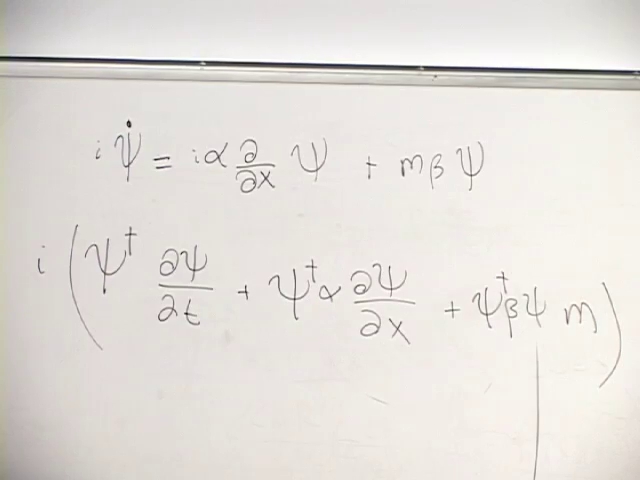
\includegraphics[width=0.76\textwidth]{lecture_09_figure_05.png}
\caption{حدود المشتقة الزمنية والمشتقة المكانية والكتلة في مناقشة حقل ديراك.}
\lectureframe{00:25:37}
\end{figure}

\begin{classroomqa}
\lecturetimestamp{00:26:37}
\audiencequestion{هل وُضع القوس في لاغرانجية ديراك المقترَحة في موضعه الصحيح، بحيث يضرب \(i\) التعبير بأكمله؟}
\lecturerresponse{لا يُبتّ هنا في هذا الموضع بثقة، وليس ذلك لازمًا للنقطة البنيوية: توجد لاغرانجية تولِّد معادلة ديراك.}
\end{classroomqa}

أضِف الآن مجالًا قياسيًا \(\phi\). إن الجداء الساذج \(\Psi^\dagger\Psi\,\phi\) ليس قياسيًا لورنتزيًا. وإدخال مصفوفة ديراك نفسها التي تظهر في حد الكتلة يعطي
\begin{equation}
\mathcal L_{\mathrm{int}}
\propto
\Psi^\dagger\beta\Psi\,\phi.
\end{equation}
وبصورة مكافئة، فإن \(\Psi^\dagger\beta\Psi\) هو الثنائي الخطي الديراكي القياسي. وعند مغايرة اللاغرانجية الكاملة يُضاف حد متناسب مع \(\phi\) إلى معادلة ديراك، ويُضاف مصدر متناسب مع \(\Psi^\dagger\beta\Psi\) إلى معادلة المجال القياسي. ويشتت كلٌّ من المجالين الآخر.

\begin{classroomqa}
\lecturetimestamp{00:28:03}
\audiencequestion{هل إن \(\beta\) المُدخلة في تآثر القياسي--الفرميوني هي \(\beta\) نفسها التي تظهر في حد كتلة ديراك؟}
\lecturerresponse{نعم. إنها مصفوفة ديراك نفسها.}
\end{classroomqa}

إن المقارنة
\begin{equation}
m\Psi^\dagger\beta\Psi
\qquad\hbox{and}\qquad
\Psi^\dagger\beta\Psi\,\phi
\end{equation}
تجعل الاقتران يبدو كما لو أنه معلمة كتلة استُبدلت بمجال قياسي. وسيعود هذا الملحظ عندما يُنظر قرب النهاية في مجال ذي قيمة فراغية غير صفرية.

حتى الآن كان التفسير كلاسيكيًا: تشتت الحزم الموجية حزمًا موجية أخرى. ولهذا الجبر نفسه معنى جسيمي أوضح حين تصبح الحقول مؤثرات.

\section{ما الذي تفعله أُسُس الحقول الكمومية}

يحتوي المجال الكمومي القياسي الحقيقي على مؤثرات الإنشاء والإفناء معًا. وعلى نحو تخطيطي،
\begin{equation}
\phi(x)\sim A^+(x)+A^-(x),
\end{equation}
حيث إن \(A^+\) ينشئ كمًّا و\(A^-\) يفني كمًّا. وعليه، يحتوي \(\phi^3(x)\) على أربعة أنواع من العمليات الموضعية:
\begin{equation}
\phi^3
\sim
(A^+)^3+(A^+)^2A^-+A^+(A^-)^2+(A^-)^3,
\end{equation}
حيث أُهملت في هذه القراءة التخطيطية تفاصيل الترتيب والمعاملات العددية. والتغيّرات الأربعة في عدد الجسيمات هي
\begin{equation}
3\longrightarrow0,
\qquad
0\longrightarrow3,
\qquad
2\longrightarrow1,
\qquad
1\longrightarrow2.
\end{equation}
وتؤثر عوامل المجال الثلاثة جميعًا في النقطة نفسها \(x\). ولذلك فإن حدًا تكعيبيًا واحدًا يضم إفناء ثلاثة جسيمات، وإنشاء ثلاثة جسيمات، واندماج كمّين في كمّ واحد، وانقسام كمّ واحد إلى كمّين. وفي سعة فيزيائية قد يُستبعد بعض هذه القراءات الموضعية لاحقًا بفعل حفظ الطاقة--الزخم، لكنها كلها موجودة في جداء المؤثرات نفسه.

للحدود الحرة التربيعية دور مختلف. أولًا، لِنُهمِل عامل تطبيع الفرق بين النقطتين المتجاورتين \(x\) و\(x'\):
\begin{equation}
\partial_x\phi
\ \propto\
\phi(x)-\phi(x').
\end{equation}
ويعطي التربيع والتوسيع بنية الحدود
\begin{align}
\frac12(\partial_x\phi)^2
&\ \propto\
\frac12\bigl[\phi(x)-\phi(x')\bigr]^2
\\
&=
\frac12\phi(x)^2
+\frac12\phi(x')^2
-\phi(x)\phi(x').
\end{align}
ولكل مربع عند النقطة نفسها عدة قراءات على مستوى المؤثرات: فقد ينشئ كمّين، أو يفني كمّين، أو يفني كمًّا ويعيد إنشاءه في تلك النقطة نفسها. وهذه الحدود لا تنقل جسيمًا. ويمكن للحد المتقاطع أن يفني كمًّا عند \(x'\) ويُنشئه عند \(x\)، أو بالعكس. ولذلك فهو يعمل حدَّ قفز بين أقرب الجيران. وتنقل العوامل المتكررة جسيمًا من \(x\) إلى \(x'\)، ثم إلى \(x''\)، وهكذا. وتحكم حدود المشتقة التربيعية الانتشار الحر؛ أما الحدود التكعيبية وما فوقها فتشتت الجسيمات وتُنشئها وتفنيها.

\begin{classroomqa}
\lecturetimestamp{00:36:07}
\audiencequestion{هل ينبغي أن يتضمن تمثيل المشتقة بالفروق المنتهية الفاصل \(x-x'\)؟}
\lecturerresponse{نعم. إذا سُمِّي هذا الفاصل \(L\) ظهر العامل \(L^{-2}\) بعد تربيع الفرق. وهذا العامل العددي يغيّر المعامل، لا تفسير القفز.}
\end{classroomqa}

وتعطي استعادة الفاصل
\begin{align}
\frac12(\partial_x\phi)^2
&\longrightarrow
\frac{1}{2L^2}\bigl[\phi(x)-\phi(x')\bigr]^2
\\
&=
\frac{1}{2L^2}\phi(x)^2
+\frac{1}{2L^2}\phi(x')^2
-\frac{1}{L^2}\phi(x)\phi(x').
\end{align}

حد الكتلة تربيعي أيضًا، لكنه لا يحتوي على مشتقة:
\begin{equation}
\frac12m^2\phi(x)^2.
\end{equation}
وقراءته أحادية الجسيم هي أن كمًّا واردًا يُمتص ثم يُعاد إصداره عند النقطة نفسها. وهو لا ينقل الكم؛ بل يزن وجوده هناك، أو بهذا المعنى يعدّه. ويحتوي مربع المؤثر نفسه أيضًا على قراءتي الإنشاء المزدوج والإفناء المزدوج. لذا فالتمييز المرتبط بالحركة هو بين حد تبادلي يصل بين نقطتين متجاورتين وإدراج كتلة يعمل داخل نقطة واحدة.

\section{الرأس الموضعي في الكهروديناميكا الكمية}

هذه الرسوم التخطيطية الأولية لعمليات الجسيمات هي بدايات مخططات فاينمان. والمثال المركزي هو الكهروديناميكا الكمية، وهي نظرية الإلكترونات والبوزيترونات والفوتونات.

لمعادلة ديراك أنماط ذات طاقة موجبة وأخرى ذات طاقة سالبة. وفي الاصطلاح الأقدم، يحتوي \(\Psi\) على مؤثرات إفناء لكلا نوعي الأنماط، بينما يحتوي \(\Psi^\dagger\) على مؤثرات الإنشاء المناظرة. وتُعادُ إعادةُ تفسير إزالة إلكترون ذي طاقة سالبة على أنها إنشاء بوزيترون ذي طاقة موجبة. وبعد إعادة التسمية هذه، يكون التحليل التخطيطي المفيد هو
\begin{align}
\Psi
&\sim
C^-_{e^-}+C^+_{e^+},
\\
\Psi^\dagger
&\sim
C^+_{e^-}+C^-_{e^+}.
\end{align}
وهكذا فإن \(\Psi\) يفني إلكترونًا أو ينشئ بوزيترونًا، بينما ينشئ \(\Psi^\dagger\) إلكترونًا أو يفني بوزيترونًا. ولا يُقصد بهذا الاختصار أي عامل تطبيع أو مؤشر لف مغزلي أو تكامل على الزخم.

يقترن تآثر الكهروديناميكا الكمية بتيار ديراك مع الكمون المتجهي الكهرومغناطيسي. وفي ترميز المركبات المستعمل هنا، تكون بنيته
\begin{equation}
\mathcal L_{\mathrm{QED,int}}
\sim
e\left(
\Psi^\dagger\Psi\,A_0
+
\Psi^\dagger\boldsymbol{\alpha}\Psi\mathbin{\boldsymbol{\cdot}}\mathbf A
\right),
\end{equation}
حيث
\begin{equation}
J^0=\Psi^\dagger\Psi,
\qquad
\mathbf J=\Psi^\dagger\boldsymbol{\alpha}\Psi.
\end{equation}
والرمز \(\sim\) مهم: فالإشارة النسبية بين الحدين الزمني والمكاني تعتمد على اصطلاحي المتريّة والكمون المتجهي. أما العبارة الثابتة فهي أن التيار الرباعي يُعقَد مع الكمون الرباعي.\editorialnote{يحدد المصدر المركبتين الزمنية والمكانية للتيار، لكنه لا يحسم اصطلاحًا للمتريّة في عقد المركبات.}

يحتوي حقل الفوتون \(A_\mu\) نفسه على مؤثرات إنشاء الفوتونات وإفنائها. كما أن طبيعته المتجهية تحمل أيضًا استقطاب الفوتون---أي ``علامة'' اتجاهية صغيرة بالإضافة إلى زخمه.

\begin{classroomqa}
\lecturetimestamp{00:44:28}
\audiencequestion{كيف يمكن أن يكون التآثر قياسيًا بينما يكون \(A_\mu\) متجهًا ويبدو عامل الفرميون في البداية كمية قياسية؟}
\lecturerresponse{توفر الفرميونات أيضًا متجهًا رباعيًا: \(\Psi^\dagger\Psi\) هو مركبته الزمنية و\(\Psi^\dagger\boldsymbol\alpha\Psi\) مركبته المكانية. وعقد ذلك التيار مع \(A_\mu\) ينتج كمية قياسية.}
\end{classroomqa}

بضرب المحتوى المؤثري لـ \(\Psi^\dagger\) و\(\Psi\) و\(A_\mu\) نحصل على أربعة تفسيرات مألوفة لرأس موضعي واحد:
\begin{enumerate}
\item يصدر إلكترون فوتونًا؛
\item يمتص إلكترون فوتونًا؛
\item يفنى إلكترون وبوزيترون في فوتون؛
\item يُنشئ فوتون زوج إلكترون--بوزيترون.
\end{enumerate}
في التفسير الأول، يفني \(\Psi\) الإلكترون الوارد، وينشئ \(\Psi^\dagger\) الإلكترون الصادر، وينشئ حقل الفوتون الفوتون. واختيار جزء إفناء الفوتون يعطي الامتصاص. واختيار الأجزاء الخاصة بالبوزيترون يعطي فناء الزوج أو إنشاء الزوج. ويحتوي حد موضعي واحد العائلة كلها.

في مخطط تدفق الفرميونات، يشير السهم على خط البوزيترون عكس اتجاه انتشار البوزيترون. وبهذا الاصطلاح يمر سهم الفرميون بلا انقطاع عبر كل رأس مسموح به في الكهروديناميكا الكمية. وتختلف التفسيرات الأربعة بنقل الأرجل الخارجية بين جانبي الوارد والصادر، لا بكسر خط تدفق الفرميون.

كل واحد من هذه التفسيرات يحمل المعامل نفسه \(e\)، وهو الشحنة الكهربائية في الاصطلاح المجهري المستعمل. وهذا المعامل هو الشحنة الكهربائية \(e\)، وليس ثابت البنية الدقيقة، مع أن كليهما مرتبط بالآخر ارتباطًا وثيقًا. وسعة الرأس تتناسب مع \(e\)؛ وبعد إدراج جميع العوامل الحركية وعوامل التطبيع، يتناسب مقياس الاحتمال الموافق مع \(e^2\).

\begin{classroomqa}
\lecturetimestamp{00:49:44}
\audiencequestion{هل لتفسير فوتون إلى إلكترون--بوزيترون المعامل نفسه مثل سائر تفسيرات الرأس؟}
\lecturerresponse{نعم. فهو يحمل معامل الشحنة الكهربائية نفسه \(e\).}
\end{classroomqa}

\begin{classroomqa}
\lecturetimestamp{00:49:59}
\audiencequestion{هل لا بد من وجود عامل تحجيم، بما أن الاحتمال لا وحدة له؟}
\lecturerresponse{في الاصطلاح المجهري الطبيعي المستخدم هنا، تكون الشحنة \(e\) عديمة الأبعاد. فهي مقياس السعة، بينما يمد مربعها بمقياس الاحتمال.}
\end{classroomqa}

وصورة ملموسة لذلك هي إلكترون يصطدم بجدار ويتوقف فجأة. وهناك بعض الاحتمال لأن تغادر الطاقة والزخم على هيئة فوتون. والعامل الكهرومغناطيسي الأولي في سعة هذا الإشعاع هو \(e\)، لذا فإن مقياس احتماله يحتوي على \(e^2\). وهذه العبارة تعزل عامل الاقتران؛ فالاحتمال الفعلي يعتمد أيضًا على حالة الإلكترون وعلى الحركيات.

\begin{figure}[htbp]
\centering
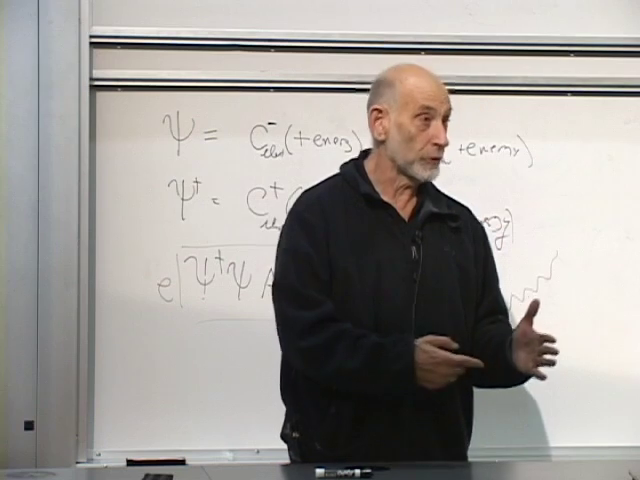
\includegraphics[width=0.78\textwidth]{lecture_09_figure_06.png}
\caption{محتوى مؤثرات الإلكترون والبوزيترون في \(\Psi\) و\(\Psi^\dagger\)، مع رسم تخطيطي لتآثر إلكترون--فوتون.}
\lectureframe{00:50:39}
\end{figure}

\begin{classroomqa}
\lecturetimestamp{00:51:15}
\audiencequestion{هل للشحنة الكهربائية وحدات؟}
\lecturerresponse{ليس في الاصطلاح المجهري الطبيعي المستخدم هنا. فكثيرًا ما تُعطى الشحنة العيانية بالكولوم، لكن نظرية الجسيمات تقيس الشحنة نسبةً إلى وحدة أولية مختارة. وفي وحدات بلانك أو غيرها من الوحدات الطبيعية تُعبَّر الكميات على هيئة أعداد محضة.}
\end{classroomqa}

يكمن التباين في الاصطلاحات والمقاييس. فالكولوم ملائم للتيار في الأسلاك؛ والاقتران العديم الأبعاد ملائم للسعات المجهرية.\editorialnote{سؤال موجز من 00:52:37--00:53:15 حول ``تجميع'' الحدود الحاملة للشحنة تالف إلى حد كبير، ولم يفض إلى صياغة محددة.}

تُقيَّم الحقول الثلاثة جميعًا في التآثر الأولي للكهروديناميكا الكمية عند نقطة واحدة في الزمكان. ولا يُسنَد إلى الرأس نفسه أي تأخر زمني داخلي.

\begin{classroomqa}
\lecturetimestamp{00:53:19}
\audiencequestion{هل يكون امتصاص الإلكترون وإعادة إصداره وانبعاث الفوتون متزامنة، أم أن المعادلة تُضمّن تأخرًا؟}
\lecturerresponse{في الرأس الأولي تُقيَّم جميع المؤثرات عند النقطة نفسها من الزمكان. لذلك لا تتضمن العملية الأساسية أي تأخر بين تلك الأفعال.}
\end{classroomqa}

\begin{classroomqa}
\lecturetimestamp{00:53:57}
\audiencequestion{هل يجب أن تُحفظ كل كمية محفوظة على حدة؟}
\lecturerresponse{نعم. والشحنة الكهربائية إحدى الكميات التي يجب أن تُحفظ على حدة.}
\end{classroomqa}

يظهر حفظ الشحنة في كل من المخطط والجبر. فالعملية التي تحوِّل إلكترونًا واردًا إلى بوزيترون صادر تقلب الشحنة، وليست رأسًا مسموحًا به في الكهروديناميكا الكمية. وعندما يُرسم الزمن إلى الأعلى، يتبع سهم الإلكترون اتجاه الزمن إلى الأعلى ويشير سهم البوزيترون إلى الأسفل؛ ويكون في الرأس الصحيح دائمًا سهم فرميوني يمر عبره. جبريًا، يحتوي التآثر على \(\Psi\) واحد و\(\Psi^\dagger\) واحد. فالأول يرفع الشحنة بمقدار وحدة واحدة عندما يفني إلكترونًا أو ينشئ بوزيترونًا، والثاني يخفضها بمقدار وحدة واحدة. وتتلاشى آثارهما.

\begin{classroomqa}
\lecturetimestamp{00:56:05}
\audiencequestion{هل التعبير المؤطر للإلكترون--الفوتون هو لاغرانجيان الكهروديناميكا الكمية كله؟}
\lecturerresponse{لا. إنه حد التآثر. ولم تُكتب الحدود الحرة التربيعية للفوتون ولا حدود ديراك التربيعية التي تحكم الانتشار.}
\end{classroomqa}

\begin{classroomqa}
\lecturetimestamp{00:56:35}
\audiencequestion{هل يُستنتج لاغرانجيان كلاسيكي بينما يُخمَّن لاغرانجيان كمي ويُختبر، وهل تبقى بنية الحركية ناقص الجهد في ميكانيكا الكم؟}
\lecturerresponse{يبقى نمط الحركية ناقص الجهد: فمشتقات الزمن تعطي الصورة الحركية، وتعممها التدرجات المكانية، وتعطي حدود الحقول غير المشتقة الصورة الجهدية. ولاغرانجيان الكمي هو الوصف الأكثر أساسية. وفي حالة تحتوي عددًا كبيرًا جدًا من الكمات، ينتج لاغرانجيان نفسه معادلات الموجات الكلاسيكية. وتُقترح اللاغرانجيانات المرشحة باستخدام المبادئ الفيزيائية ونظرية أعمق، ثم تُثبَت أو تُرفَض عبر تجارب التصادم.}
\end{classroomqa}

يفسر حد الإشغال الكبير لماذا يمكن للتعبير نفسه أن يحكم نظرية جسيمات كمية وموجاتها الكلاسيكية. وهذا التوافق ليس معجزة مستقلة فُرضت بعد ذلك؛ فالحقل الكلاسيكي هو السلوك الجمعي لعدد كبير من الكمات. وعلى العكس من ذلك، تكشف التصادمات التجريبية الرؤوس الأولية مباشرةً بما يكفي لتحديد تآثرات الكهروديناميكا الكمية والنموذج المعياري بدقة كبيرة.

\section{العبور وقوانين الحفظ في الزمكان}

يمكن تبديل أرجل رأس موضعي بين موضعي الداخل والخارج. فالجسيم الخارج الذي يُنقل إلى جهة الداخل يُعاد تفسيره على أنه جسيمه المضاد، وبالعكس. وبهذا المعنى فإن مؤثر الإلكترون--البوزيترون--الفوتون نفسه له قراءة موضعية على أنها انبعاث، وامتصاص، وفناء زوجي، وخلق زوجي، وحتى قراءة يكون فيها الجميع داخلين.

\begin{classroomqa}
\lecturetimestamp{00:59:34}
\audiencequestion{إذا أُدير مخطط رأس أساسي، فهل يظل قراءة موضعية صحيحة؟}
\lecturerresponse{نعم. يمكن نقل أرجله الخارجية بين موضعي الداخل والخارج، مع إعادة التفسير المناظرة للجسيم--الجسيم المضاد.}
\end{classroomqa}

القراءة المؤثرية الموضعية ليست بعدُ عملية فيزيائية مكتملة. ويجب تكامل سعتها على كل نقطة في الزمكان يمكن أن يحدث عندها الرأس. فتكامل الزمن يفرض حفظ الطاقة، وتكامل المكان يفرض حفظ الزخم. والصورة التي يختفي فيها إلكترون وبوزيترون وفوتون جميعًا في الفراغ موجودة بوصفها قراءة موضعية صورية، لكن السعة المتكاملة تنعدم لأن العملية لا يمكنها أن تحفظ الطاقة والزخم.

\begin{classroomqa}
\lecturetimestamp{01:00:30}
\audiencequestion{هل تعني الصورة التي يكون فيها الجميع داخلين أن إلكترونًا وبوزيترونًا وفوتونًا يمكن أن يختفوا في العدم؟}
\lecturerresponse{إنها قراءة للمؤثر الموضعي، لكن السعة الفيزيائية تتضمن تكاملًا على موضع الرأس. وتفرض تلك التكاملات حفظ الطاقة والزخم، لذا فهذه العملية الممنوعة حركيًا سعتها صفر.}
\end{classroomqa}

\begin{classroomqa}
\lecturetimestamp{01:01:57}
\audiencequestion{وهل توجد أيضًا القراءة العكسية من الفراغ إلى إلكترون--بوزيترون--فوتون، وهل تختفي العمليات المستبعَدة بعد التكامل؟}
\lecturerresponse{القراءة الموضعية العكسية موجودة أيضًا. والتكامل على المكان والزمان يزيل أي عملية لا تنسجم مع قوانين الحفظ.}
\end{classroomqa}

تنسجم المشتقات في اللاغرانجيان مع التوسع المؤثري من غير أن يُشتق رمزا الخلق والفناء نفسيهما. وللحقل الصورة التخطيطية
\begin{equation}
\Psi(x)
\sim
\int d^3k\,
\bigl[
C(\mathbf k)e^{i\mathbf k\cdot\mathbf x-i\omega t}
+\cdots
\bigr].
\end{equation}
والمؤثرات \(C(\mathbf k)\) هي معاملات في هذا التوسع الزمكاني. وتؤثر المشتقات في الموجات المستوية فتُنزل \(\mathbf k\) أو \(\omega\).

\begin{classroomqa}
\lecturetimestamp{01:02:27}
\audiencequestion{عند اشتقاق توسع حقل، هل يُشتق مؤثر الخلق نفسه؟}
\lecturerresponse{لا. مؤثرا الخلق والفناء مستقلان عن إحداثي الزمكان في هذا التوسع. وتؤثر المشتقات في العوامل الأسية وتُنزل الزخم والتردد.}
\end{classroomqa}

\section{النيوكليونات والبيونات بوصفها نظرية فعالة}

يمكن للغة نفسها أن تصف البروتونات والنيوترونات والبيونات. فالبروتونات والنيوترونات فرميونات تمثلها الحقول \(\Psi_p\) و\(\Psi_n\). وفي هذا النقاش الخاص بعدّ التفاعلات، تُعامَل حقول البيون على أنها حقول قياسية بثلاثة أصناف من الشحنة،
\begin{equation}
\pi^+,
\qquad
\pi^-,
\qquad
\pi^0.
\end{equation}
يحمل البروتون و\(\pi^+\) وحدة موجبة واحدة من الشحنة الكهربائية، ويحمل \(\pi^-\) وحدة سالبة واحدة، أما النيوترون و\(\pi^0\) فمتعادلَان. وعلى مستوى أعمق، البيونات منظومات كوارك--ضديد كوارك، لكن يمكن في البداية ترك هذا الوصف الداخلي دون حسم.

قائمة تخطيطية محافظة على الشحنة لجداءات حقول النيوكليون--البيون هي
\begin{equation}
\mathcal L_{N\pi}
\sim
\left\{
\Psi_p^\dagger\Psi_n\,\pi^+,\;
\Psi_n^\dagger\Psi_p\,\pi^-,\;
\Psi_p^\dagger\Psi_p\,\pi^0,\;
\Psi_n^\dagger\Psi_n\,\pi^0
\right\}.
\end{equation}
المعروض هنا هو فقط محتوى الحقول وإسنادات الشحنة؛ أما المعاملات النسبية، والإشارات، وبنية المصفوفة السبينورية، فلا تُثبَّت هنا. وتتحدد شحنة حقل البيون الأول باختبار قراءة محددة: فبإمكان نيوترون مع بيون موجب أن ينتجا بروتونًا، بينما استعمال بيون سالب هناك من شأنه أن يحول شحنة داخلة سالبة إلى شحنة خارجة موجبة. ويعطي الحد المرافق العملية ذات الشحنة المعاكسة.\editorialnote{صُحِّحت إشارة البيون عدة مرات في المصدر قبل الوصول إلى الزوج المحافظ على الشحنة المعروض هنا؛ والترتيب المعروض يسجل تلك البنية التخطيطية النهائية.}

ولكل حد مرة أخرى عدة قراءات متقاطعة. فنقل نيوترون خارج إلى جهة الداخل يحوله إلى ضديد نيوترون داخل. ولذلك يمكن للرأس المشحون أن يصف بروتونًا وضديد نيوترون يتحدان في \(\pi^+\)، وكذلك عمليات مثل \(p\to n+\pi^+\) عندما تسمح الحركيات بذلك. وتتيح الحدود المتعادلة لبروتون أو نيوترون أن يصدر أو يمتص \(\pi^0\). ويختار حفظ الشحنة العائلة المسموح بها، بينما تحدد الطاقة والزخم وأي تناظرات إضافية أيَّ فرد منها يمكن أن يقع في تجربة معينة.

كان هذا وصفًا فعالًا مفيدًا قبل أن تُعرف البنية التحتية الكواركية. وما يزال مفيدًا كلما عجز المسبار عن تمييز تلك البنية. فللبروتون توزع متناهٍ في الامتداد لمكوناته، على نحو يشبه امتلاك الذرة بنية داخلية، وإن كان على مقياس أصغر بكثير. وإذا نقلت تجربة زخمًا قليلًا جدًا بحيث لا يكفي لتفكيك البروتون أو تمييزه، أمكن معاملة البروتون بوصفه جسيمًا نقطيًا له حقله الخاص. أما التصادم الشديد بما يكفي فيكشف الكواركات، وعندئذٍ لا يعود حقل البروتون الجسيمي النقطي كافيًا.

ولأن البروتون مشحون، فله أيضًا تآثر موضعي بروتون--فوتون، تخطيطيًا \(J_p^\mu A_\mu\)، حيث إن \(J_p^\mu\) هو تيار البروتون. وللإلكترون تآثره المناظر إلكترون--فوتون. ولا يمكن للبروتون بدلًا من ذلك أن يتحول إلى نيوترون بإصدار فوتون: إذ إن \(p\to n+\gamma\) ينتهك حفظ الشحنة.

\begin{classroomqa}
\lecturetimestamp{01:10:28}
\audiencequestion{ماذا يحدث عندما يتآثر بروتون وإلكترون؟}
\lecturerresponse{لكل جسيم مشحون رأس فوتون. يمكن للبروتون أن يصدر فوتونًا مع بقائه بروتونًا، ويمكن للإلكترون أن يمتص الفوتون مع بقائه إلكترونًا. ويُبنى تشتت البروتون--الإلكترون من هذين الرأسين الموضعيين وانتشار الفوتون بينهما.}
\end{classroomqa}

\section{الموضعية والعمليات الأولية المتكررة}

لا يوجد حد لا موضعي خاص للتبادل الكامل بروتون--إلكترون. فرأس موضعي واحد يصدر الفوتون عند البروتون، وتنقله الحدود التربيعية للفوتون من نقطة مجاورة إلى نقطة مجاورة، ويمتصه رأس موضعي آخر عند الإلكترون. والعملية الممتدة هي حاصل ضرب تلك القطع الأولية.
\begin{equation}
\begin{aligned}
\bigl[J_p^\mu A_\mu\bigr](x_p)
&\longrightarrow
\underbrace{x_p\to x_1\to x_2\to\cdots\to x_e}_{\text{quadratic photon propagation}}
\\
&\longrightarrow
\bigl[J_e^\nu A_\nu\bigr](x_e).
\end{aligned}
\end{equation}
والأسهم في هذه السلسلة التخطيطية تدل على إدخالات متعاقبة بين نقاط متجاورة، لا على تآثر لا موضعي جديد.

\begin{classroomqa}
\lecturetimestamp{01:12:06}
\audiencequestion{كيف يكتب المرء اللاغرانجيان للتبادل الكامل بروتون--إلكترون؟}
\lecturerresponse{لا يضاف حد للحدث الممتد كله. بل يُبنى من رأس موضعي بروتون--فوتون، وحدود انتشار تربيعية متكررة، ورأس موضعي إلكترون--فوتون.}
\end{classroomqa}

للبنية الموضعية صورتان. فحد التآثر غير المشتق يؤثر عند نقطة واحدة في الزمكان. أما الحد المشتق، المعبَّر عنه بفارق منتهٍ، فيصل تلك النقطة بنقطة مجاورة فقط. ولا ينقل أي من النوعين جسيمًا مباشرة عبر مسافة منتهية. فالانتشار بعيد المدى يُركَّب من انتقالات متناهية الصغر كثيرة؛ ولا يوجد تأثير أولي عن بُعد.

\begin{classroomqa}
\lecturetimestamp{01:14:36}
\audiencequestion{هل يحتوي اللاغرانجيان على حدود عند نقطة واحدة فقط؟}
\lecturerresponse{تؤثر حدود التآثر عند نقطة واحدة. أما الحدود المشتقة فتصل نقطة بنقطة مجاورة لها على نحو متناهٍ في القرب. ويؤدي الإصدار، ثم القفزات الكثيرة بين النقاط المتجاورة، ثم الامتصاص معًا إلى تبادل منتهٍ.}
\end{classroomqa}

\begin{classroomqa}
\lecturetimestamp{01:15:36}
\audiencequestion{هل جميع قطع العملية الممتدة موجودة، وهل يعني تركيبها أخذ حاصل ضربها؟}
\lecturerresponse{نعم. فكل إصدار أولي، أو قفزة، أو امتصاص، مُرمَّز له في اللاغرانجيان. وتُركِّب جداءات الإدخالات المتكررة تلك القطع في العملية الأكبر.}
\end{classroomqa}

تفترض نظرية الحقل الكمومي النسبية قيد المناقشة الإطار الزمكاني الذي تُعرَّف عليه حقولها. ولا ينبغي الخلط بينها وبين نظرية كمومية كاملة لهندسة زمكانية ديناميكية.

\begin{classroomqa}
\lecturetimestamp{01:16:28}
\audiencequestion{هل يظل هذا التركيب صالحًا في وضع نسبي شديد، مثل القرب من أفق ثقب أسود؟}
\lecturerresponse{امتداد ذلك إلى حالة الثقب الأسود خارج نطاق هذا البناء. فنظرية الحقل الكمومي المستعملة هنا لا توفر بذاتها وصفًا كاملًا لديناميكيات الثقوب السوداء، حيث تكون الجاذبية أساسية.}
\end{classroomqa}

الحقل مؤثر لفعل موضعي أولي. ويمكن لعامل حقلي واحد أن يمتص جسيمًا أو أن يصدر جسيمًا. ويمكن لجداء عاملين أن يمتص جسيمًا ويصدر آخر عند النقطة نفسها؛ كما تستطيع الجداءات الأعلى رتبة أن تغير محتوى الجسيمات أكثر. وتصل جداءات المؤثرات الموضعية هذه الأفعال في تواريخ. وفي الزمكان تُمثَّل الحركة بامتصاص في منطقة صغيرة، ثم إعادة إصدار إلى منطقة مجاورة، ثم امتصاص آخر، ثم إعادة إصدار أخرى. وجعل طول الخطوة يقترب من الصفر مع ازدياد عدد الخطوات يعطي المسار المتصل.

\begin{classroomqa}
\lecturetimestamp{01:17:30}
\audiencequestion{كيف ينبغي فهم الحقول والمسافة والزمن في هذه الصورة القائمة على الخطوات المحلية؟}
\lecturerresponse{الحقول هي مؤثرات للامتصاص والإصدار المحليين. وتربط المضروبات بين تلك الأفعال الأولية، وتُبنى الحركة عبر الزمكان من خطوات متناهية الصغر بين المواضع المتجاورة قبل أخذ حد المتصل.}
\end{classroomqa}

ولذلك فإن نقطة بداية منظَّمة هي تقسيم الزمكان إلى خلايا صغيرة، مع إلحاق مؤثرات الحقل بالخلايا.\editorialnote{صياغة الحضور عند 01:17:30--01:20:40 محجوبة جزئياً؛ والسؤال المعاد بصياغته لا يحتفظ إلا بموضوعه الذي أمكن استرجاعه، بينما الجواب عن المؤثرات المحلية وخطوات الزمكان المتعاقبة واضح.} وتتحول المشتقات إلى فروق. وتصل الحدود التربيعية المختلطة بين الخلايا المتجاورة، بينما تؤثر حدود الكتلة والتفاعل داخل خلية واحدة. والخلايا أداة لتعريف النظرية الحدية، وليست جسيمات إضافية ولا مقياساً فيزيائياً جديداً للكتلة.

لا يلزم أن تُضاف تأثيرات النسبية الخاصة على نحو منفصل في كل خطوة. فإذا كان اللاجرانجي كمية قياسية لورنتزية، فإن السعات المجمَّعة منه تكون ثابتة تحت تحولات لورنتز، وتترتب تأثيرات مثل تمدد الزمن على تلك البنية.

\begin{classroomqa}
\lecturetimestamp{01:21:10}
\audiencequestion{هل تخلق الحركة عالية الطاقة وتمدد الزمن مشكلات إضافية في عملية متعددة الخطوات؟}
\lecturerresponse{لا يلزم تصحيح منفصل. فإذا كان اللاجرانجي كمية قياسية لورنتزية، فإن تأثيرات النسبية الخاصة مثل تمدد الزمن مدمجة بالفعل في النتيجة. أما منشأ القلق المحدد الكامن وراء السؤال فليس واضحاً تماماً.}
\end{classroomqa}

يمكن تمثيل مؤثرات الإنشاء والإفناء في أساس الموضع أو في أساس الزخم. ومؤثر الإنشاء في فضاء الموضع هو تراكب فورييه لمؤثرات الإنشاء في فضاء الزخم، وبالعكس. ولا يوجد مؤثر ينشئ حالة يكون فيها الموضع محدداً بدقة والزخم محدداً بدقة في آن واحد. فتوطين الجسيم على نحو حاد يتطلب نطاقاً واسعاً من الزخوم؛ وتوطينه على نحو حاد في الزخم ينشره على الموضع. وعلاقة فورييه بين الأساسين هي مبدأ عدم اليقين بهذه اللغة.

\begin{classroomqa}
\lecturetimestamp{01:22:48}
\audiencequestion{كيف ترتبط مؤثرات الإنشاء والإفناء بالموضع والزخم ومبدأ عدم اليقين؟}
\lecturerresponse{يمكن تمثيلها بوصفها توابع للموضع أو توابع للزخم. والتمثيلان تحويل فورييه أحدهما للآخر. فالحالة الحادة التوضع في الموضع تتطلب كثيراً من الزخوم، بينما تكون الحالة الحادة في الزخم ممتدة على الموضع؛ ولا يوجد مؤثر إنشاء لـ \(x\) و\(p\) محددين بحدة في آن واحد.}
\end{classroomqa}

يمكن الآن صياغة بناء الخلايا بالكامل. وسِم الخلايا بـ \(n\)، واستبدل المشتق بفارق منتهٍ مثل
\begin{equation}
\partial_\mu\phi(x)
\longrightarrow
\frac{\phi_{n+\hat\mu}-\phi_n}{a},
\end{equation}
وضع كل نوع حقلي في كل خلية. حد تربيعي مختلط يزيل كمّاً من خلية ويُنشئه في خلية مجاورة. وتُستعاد نظرية المتصل بأخذ التباعد \(a\) نحو الصفر بعد تعريف التعابير المنظَّمة.
\begin{equation}
\underbrace{\phi_n\phi_{n+\hat\mu}}_{\text{hop }n\leftrightarrow n+\hat\mu},
\qquad
\underbrace{m^2\phi_n^2}_{\text{same-cell mass insertion}}.
\end{equation}

\begin{classroomqa}
\lecturetimestamp{01:25:16}
\audiencequestion{هل يمكن إتمام تقسيم الزمكان إلى خلايا؟}
\lecturerresponse{نعم. تُفهرس الحقول بالخلايا، وتتحول المشتقات إلى فروق منتهية، وتنقل الحدود التربيعية الجسيمات قفزاً بين الخلايا المتجاورة. ويُستعاد المتصل عندما يؤول حجم الخلية إلى الصفر.}
\end{classroomqa}

تقفز الإلكترونات بين الخلايا عبر حدودها التربيعية، وكذلك تفعل الفوتونات. وعندما يجتمع إلكترون وفوتون في خلية واحدة، يمكن لتفاعل QED أن يمتص الإلكترون ويعيد إصداره مع إنشاء الفوتون أو إفنائه. ولحد الكتلة القياسي قراءة داخل الخلية نفسها: يدخل الجسيم تلك الخلية ويغادرها بمعامل يتناسب مع \(m^2\). وهو لا يوفّر قفزة.

\begin{classroomqa}
\lecturetimestamp{01:28:18}
\audiencequestion{هل يرتبط حجم الخلية بمعامل الكتلة؟}
\lecturerresponse{لا. حجم الخلية هو تباعد تنظيمي يُؤخذ في النهاية إلى الصفر؛ أما معامل الكتلة فهو وسيط مستقل في اللاجرانجي.}
\end{classroomqa}

\begin{classroomqa}
\lecturetimestamp{01:28:43}
\audiencequestion{هل ضرب العوامل المحلية هو بناء لسعة مشتركة على امتداد الزمكان، لا مجرد تعاقب زمني؟}
\lecturerresponse{نعم. تغطي الخلايا الزمكان، وتتجمع إسهاماتها المحلية عبر شبكة الزمكان تلك. ويعطي المضروب سعة مشتركة للأحداث المحلية المطلوبة وخطوات الانتشار.}
\end{classroomqa}

\section{المصادر والكواشف والديناميات بينهما}

العملية الكاملة هي تاريخ في الزمكان. ويتحدد شرطها الابتدائي بما يهيئه المجرِّب، وشرطها النهائي بما تسجله الكواشف. ومصدر بسيط هو فتيلة ساخنة تبعث إلكتروناً. فمؤثر حقلي عند الفتيلة ينشئ ذلك الإلكترون الوارد؛ ومؤثرات حقلية عند مواضع الكواشف تصف امتصاصه في نهاية المطاف.

\begin{classroomqa}
\lecturetimestamp{01:29:30}
\audiencequestion{ما المرحلة الابتدائية لمثل هذه العملية في الزمكان؟}
\lecturerresponse{تُهيَّأ عند المصادر. والإلكترون المنبعث من فتيلة ساخنة مثال بسيط: فمؤثر حقلي عند الفتيلة ينشئ الإلكترون، بينما تحدد مؤثرات حقلية عند الكواشف أحداث الامتصاص النهائية.}
\end{classroomqa}

يمكن كذلك صياغة البناء نفسه انطلاقاً من الخلاء. فمؤثرات الإنشاء عند المصادر تبني الحالة الداخلة على الخلاء. ومؤثرات الإفناء المرتبطة بالكواشف تنتقي الحالة الخارجة. وهذه المؤثرات تحدد الشروط الحدية؛ وهي لا تحل محل الديناميات في كامل المنطقة بين المصدر والكاشف.

\begin{classroomqa}
\lecturetimestamp{01:31:11}
\audiencequestion{هل يكون من الخطأ حصر الديناميات في البواعث وحدها بدلاً من امتدادها في النظام كله؟}
\lecturerresponse{نعم. ابدأ من الخلاء، واستعمل مؤثرات المصدر لتهيئة الجسيمات الداخلة، واستعمل مؤثرات الكاشف لانتقاء الجسيمات النهائية. وبينهما تعمل إدخالات اللاجرانجي المتكررة في الزمكان كله، فتنقل الجسيمات، وتنشئها، وتفنيها.}
\end{classroomqa}

ومع عدد كافٍ من الإدخالات، يمكن لعدة جسيمات أن تتحرك في آن واحد عبر كثير من الخلايا المتجاورة؛ كما يمكن إنشاء الجسيمات أو إفناؤها على طول الطريق. وتبيّن المؤثرات الابتدائية ما الذي يدخل، وتبيّن المؤثرات النهائية ما الذي يُسجَّل، وتوفر عمليات اللاجرانجي المتكررة كل ما بينهما.

\begin{classroomqa}
\lecturetimestamp{01:33:24}
\audiencequestion{إذا أمكن حدوث عدد اعتباطي من إدخالات اللاجرانجي، فهل يُكامل على مواضعها؟}
\lecturerresponse{نعم. يُكامل على مواضعها في الزمكان. ولا تُشتق قواعد فاينمان الدقيقة هنا؛ وإنما النقطة المباشرة هي أن تعابير حقلية محلية بسيطة ترمّز إلى التفاعلات الأولية التي تُركَّب منها عملية كاملة.}
\end{classroomqa}

\section{تناظر الطور والشحنة والسعات}

إن كتابة العمليات الأولية في اللاجرانجي تجعل تناظراتها مرئية أيضاً. اعتبر تحول طور شامل لحقل الإلكترون،
\begin{equation}
\Psi\longrightarrow e^{i\theta}\Psi,
\qquad
\Psi^\dagger\longrightarrow e^{-i\theta}\Psi^\dagger,
\qquad
A_\mu\longrightarrow A_\mu.
\end{equation}
فالحد الذي يحتوي على عدد متساوٍ من \(\Psi\) و\(\Psi^\dagger\) لا يتغير لأن الأطوار تتلاشى فيما بينها. أما الحد ذو العددين غير المتساويين فسيكتسب طوراً. وتساوي هذين العددين هو الصورة الجبرية لانحفاظ الشحنة.

وهذه ميزة مركزية للوصف باللاجرانجي. فعوامله الحقلية تُظهر العمليات الأولية، وتُظهر تراكيبها التناظرات، وتُظهر التناظرات قوانين الانحفاظ. وتحول الإدخالات المتكررة الحالة الابتدائية المهيأة إلى الحالة النهائية المنتقاة. والنتيجة هي سعة كمومية. ويتطلب التقييم الدقيق قواعد فاينمان، لكن المحتوى البنيوي ظاهر بالفعل: فالعمليات المحلية تتكرر بكل ترتيب تسمح به قوانين الانحفاظ.

\section{قياسات الحقول والمبدلات}

تحتفظ مؤثرات الحقل بالمعنى المعتاد للمؤثرات في ميكانيكا الكم. فقيمها الذاتية هي النتائج الممكنة لقياسات الحقل، ومتجهاتها الذاتية تصف الحالات المرتبطة بتلك القيم. ويمكن سبر مجال كهربائي بوضع جسيم مشحون فيه ومراقبة كيف يتسارع ذلك الجسيم.

\begin{classroomqa}
\lecturetimestamp{01:37:06}
\audiencequestion{هل تؤدي القيم الذاتية والمتجهات الذاتية لمؤثرات الحقل دورها المعتاد في ميكانيكا الكم؟}
\lecturerresponse{نعم. القيم الذاتية هي القيم الحقلية الممكنة في القياس، ويمكن سبر الحقول من خلال تأثيراتها في الجسيمات. وتحدد المبدلات القيود على القياسات المتزامنة.}
\end{classroomqa}

الهوية التافهة
\begin{equation}
[\phi(x),\phi(x)]=0
\end{equation}
لا تحسم مسألة القياس. فلا بد من تحديد مرصودين وعلاقتهما الزمكانية. ويشكّل الحقل وزخمه المرافق زوجًا قانونيًا لا يتبادل، ومؤثرات الحقل عند نقاط يفصل بينها فاصل زمني قد لا تتبادل؛ أما الحقول البوزونية المحلية عند فصل مكاني فتتبادل، كما تقتضيه المحلية. ومن ثم تنتقل العلاقة المألوفة بين المبدِّلات وعدم اليقين إلى هنا أيضًا، ولكن فقط بعد تعيين زوج المؤثرات تعيينًا صحيحًا.\editorialnote{يعرض المصدر عدمَ التبادل عند نقاط متميزة على نحو أوسع مما ينبغي. والتقييد الوارد هنا يحافظ على مغزاه المتعلق بالقياس مع فرض السببية الميكروية للحقول البوزونية المحلية ذات الفصل المكاني.}

\begin{classroomqa}
\lecturetimestamp{01:39:57}
\audiencequestion{هل يُقاس المجال الكهربائي أو الكهرومغناطيسي بالفولت، أم بالفولت لكل متر؟}
\lecturerresponse{يُقاس المجال الكهربائي بالفولت لكل متر. وليست الفولتات والأمتار اللغة الأكثر فائدة لعمليات الحقول المجهرية، إذ تُنظَّم على نحو أيسر من حيث الفوتونات. وعلى العكس، فإن نظرية الحقل الكمومي ليست اللغة المفيدة لتقرير كيف تسقي منزلًا.}
\end{classroomqa}

الوحدات الطبيعية لوصفٍ ما ليست بالضرورة هي الوحدات الأكثر إيضاحًا في وصفٍ آخر. فالفولت والفولت لكل متر يلائمان الأجهزة العيانية؛ أما خلق الفوتونات وإفناؤها فيلائمان العمليات المجهرية.

\begin{classroomqa}
\lecturetimestamp{01:41:10}
\audiencequestion{هل الفكرة المركزية هي أن حدود اللاغرانجيان لبنات بناء تُجمع في عمليات أكبر؟}
\lecturerresponse{نعم. تتكرر العمليات الأولية من نقطة إلى أخرى. وكل عنصر أساسي يؤثر عند نقطة واحدة في الزمكان، أو يصل بين نقاط متجاورة من خلال حد اشتقاقي. ويُبنى الانتشار الذي يبدو لا محليًا من هذه الخطوات المحلية؛ فلا يوجد فعل أولي عن بُعد.}
\end{classroomqa}

\section{حواصل ضرب العمليات المحلية والمجاميع على المسارات}

ثمة طريقة استرشادية موجزة لعرض تكرار العمليات المحلية. قسِّم الزمكان إلى خلايا واكتب
\begin{equation}
\prod_x\bigl(1+\mathcal L_I(x)\bigr),
\end{equation}
حيث يرمز \(x\) إلى الخلايا، و\(\mathcal L_I(x)\) هو لاغرانجيان التآثر المحلي. وهذه ليست الصيغة المستمرة الدقيقة. إنها بديل توافقي يكشف كيف تولِّد حواصل الضرب كل اختيار مسموح به من الأحداث المحلية.

\begin{classroomqa}
\lecturetimestamp{01:42:18}
\audiencequestion{هل يمكن اختزال كثير من خطوات الخلق والانتشار والإفناء في تعبير واحد؟}
\lecturerresponse{استرشاديًا، يُضرَب عامل واحد \(1+\mathcal L_I(x)\) لكل خلية زمكانية. ويولِّد بسط حاصل الضرب عدم وقوع أي حدث، أو وقوع حدث واحد عند أي نقطة مختارة، أو وقوع أحداث عند عدة نقاط.}
\end{classroomqa}

بالنسبة إلى خليتين،
\begin{align}
\bigl(1+\mathcal L_I(x)\bigr)
\bigl(1+\mathcal L_I(x')\bigr)
&=
1+\mathcal L_I(x)+\mathcal L_I(x')
\notag\\
&\quad{}+\mathcal L_I(x)\mathcal L_I(x').
\end{align}
يعني الحد الأول أن أيًّا من التآثرين لا يحدث. والحدان التاليان يضعان تآثرًا أوليًا واحدًا عند \(x\) أو عند \(x'\). أما الحد الأخير فيضع تآثرات عند النقطتين كلتيهما. ومع كثرة العوامل تظهر حدود تشمل نقطة واحدة، أو نقطتين، أو ثلاث نقاط، وهكذا. ويمكن لحد ذي عدة رؤوس أن يصف، على سبيل المثال، جسيمين داخلين ينتجان ثلاثة جسيمات خارجة.

تدخل الحدود التربيعية الخاصة بالانتشار في البناء نفسه. وتُمثَّل إزاحة منتهية بسلسلة من الإدراجات المتجاورة. وفي مكان ما من حاصل الضرب بعد بسطه توجد عوامل عند خلية ما، وعند جارتها، ثم الجارة التالية، وهكذا، تنقل جسيمًا بين نقطتي النهاية.

\begin{classroomqa}
\lecturetimestamp{01:46:29}
\audiencequestion{إذا كان الانتشار المنتهي يتطلب كثيرًا من حدود الحركة المحلية، فكيف تُستعاد الحركة المطلوبة؟}
\lecturerresponse{يحتوي حاصل الضرب الكبير على سلاسل من الإدراجات المتجاورة تنقل الجسيم من نقطته الابتدائية إلى نقطته النهائية. ويوجد عمومًا كثير من هذه السلاسل على مسارات مختلفة. ويسهم كل مسار بسعة، والسعة الكلية هي مجموعها.}
\end{classroomqa}

إذا كان \(r\) يرمز إلى مسار، فعلى نحو تخطيطي
\begin{equation}
\mathcal A_{\mathrm{total}}=\sum_r\mathcal A_r,
\qquad
P=\left|\mathcal A_{\mathrm{total}}\right|^2.
\end{equation}
لا تُسنَد إلى المسارات احتمالات اعتيادية ثم تُجمع. بل تُجمع السعات أولًا:
\begin{equation}
\left|\sum_r\mathcal A_r\right|^2
=
\sum_r|\mathcal A_r|^2
+
\sum_{r\ne s}\mathcal A_r\mathcal A_s^*.
\end{equation}
والحدود المتصالبة هي حدود التداخل.

\begin{classroomqa}
\lecturetimestamp{01:48:27}
\audiencequestion{هل ينسجم هذا مع تجربة الشقين؟}
\lecturerresponse{تمامًا. تسهم البدائل المارة عبر الشقين بسعات. ويُنتج تربيع مجموعها حدود تداخل، تمامًا كما تتداخل المسارات الزمكانية الكثيرة في بناء الخطوات المحلية.}
\end{classroomqa}

\begin{classroomqa}
\lecturetimestamp{01:49:00}
\audiencequestion{من أين يأتي \(1\) في كل عامل \(1+\mathcal L_I\)؟}
\lecturerresponse{إنها أداة توافقية تتيح للخلية أن تسهم بلا تآثر كما تتيح لها أن تسهم بتآثر. وهي مرتبطة بطرائق التكامل على المسارات، لكن حاصل الضرب المعروض ليس إلا تقريبًا استرشاديًا للتعبير التقني.}
\end{classroomqa}

تزود الصورية الدقيقة بالتكاملات الصحيحة على الزمكان، والترتيب، والتطبيع، والأطوار. ويكون حاصل الضرب مفيدًا لأنه يكشف التوافيق من غير أن يدّعي أنه الصياغة الكاملة.

\begin{classroomqa}
\lecturetimestamp{01:49:57}
\audiencequestion{هل هذا هو مبدأ الفعل الساكن؟}
\lecturerresponse{لا. يختار الفعل الساكن الكلاسيكي مسارًا كلاسيكيًا مميزًا. أما ميكانيكا الكم فبدلًا من ذلك تجمع السعات على المسارات، وتُحكَم أوزانها بالفعل. وحتى مسار غير مباشر إلى حد بعيد---يمر عبر باريس في الطريق من مكتب إلى منزل قريب---ينتمي إلى المجموع الكمومي.}
\end{classroomqa}

التباين بسيط، وإن كانت الصلة دقيقة. تختار الميكانيكا الكلاسيكية مسارًا ذا فعل ساكن. أما ميكانيكا الكم فتجمع على المسارات؛ وفي الحد المناسب تتعزز الأطوار حول المسار الكلاسيكي.

\section{استنباط اللاغرانجيان واختيار قطاع}

ما إن يُعطى لاغرانجيان وتُحدَّد عملية معينة حتى تكون قواعد حساب احتمالها محددة. وقد يظل إجراء الحساب يتطلب براعة، كما تفعل الرياضيات الصعبة كثيرًا، لكن اللايقين الأعمق يكمن في اكتشاف أي الحقول والاقترانات تستخدمها الطبيعة.

\begin{classroomqa}
\lecturetimestamp{01:50:43}
\audiencequestion{هل تكمن البراعة في صياغة اللاغرانجيان أم في استخدامه؟}
\lecturerresponse{تكمن البراعة الأساسية في استنباط اللاغرانجيان من المعطيات التجريبية. فحالما يُعرف، تكون لعملية مثل دخول جسيمين وخروج أربعة سعة محددة تُحسَب بقواعد دقيقة. وقد يتطلب تنفيذ الرياضيات ذكاءً، لكن ذلك ليس غموضًا في النظرية.}
\end{classroomqa}

تكشف تصادمات الجسيمات الرؤوس الأولية. وتُقترح حدود، غالبًا باسترشاد بالتناظر وبمبادئ أعمق، ثم تُختبَر السعات الناتجة بمقارنتها بالنتائج المرصودة. ويثبّت النجاح كلاً من التوافيق المسموح بها للحقول ومعاملاتها العددية.

\begin{classroomqa}
\lecturetimestamp{01:52:24}
\audiencequestion{هل يوجد لاغرانجيان منفصل لكل تآثر---كتاب كبير من اللاغرانجيانات؟}
\lecturerresponse{الصورة العملية بدلًا من ذلك هي لاغرانجيان واحد كبير يحتوي جميع الحقول والتآثرات، مع أن هذه الصورة قد تكون خاطئة في النهاية. وتظهر قطاعات يمكن تمييزها بوصفها أجزاء من المجموع. فالجسيم الجديد يضيف حقلاً؛ والعملية الأولية الجديدة تضيف حد تآثر.}
\end{classroomqa}

قد يكون التعبير الكامل غير مرتب من غير أن يبلغ طول كتاب. وعلى سبيل تقدير خشن مقصود، يمكن تخيل نحو مئة كيان تُسمى جسيمات أولية وعدة مئات من الحدود. ويمكن للديناميكا الكهربائية الكمية، والتآثرين الشديد والضعيف، وقطاع جاذبي، أن تشغل بضع صفحات مكتوبة بكثافة فحسب. وليس العدد الدقيق هو المقصود. فالصورة العملية هي تعبير ديناميكي واحد مركب من أجزاء كثيرة يمكن تمييزها، وهي صراحةً صورة قد يتبين في النهاية أنها غير مكتملة.

إن كانت الحقول تحدد هندسة زمكانية أكثر أساسية، فذلك يقع خارج الإطار المعتاد لنظرية الحقل الكمومي المستخدم هنا.\editorialnote{السؤال عند 01:55:00--01:55:20 متضرر إلى حد لا يسمح بتعيين المتشعب أو البنية الهندسية على نحو موثوق؛ وليس المضمون بثقة إلا هذا الجواب الذي يبيّن حدود النطاق.}

\begin{classroomqa}
\lecturetimestamp{01:55:22}
\audiencequestion{هل الأعداد المحددة تجريبيًا هي ثوابت الاقتران؟}
\lecturerresponse{ثوابت الاقتران هي معاملات حدود في اللاغرانجيان. والمعامل \(m^2\) لحد كتلي تربيعي مثال واحد؛ ومعاملات \(\phi^4\) و\(\phi^6\) أو قوى أعلى من ذلك أمثلة أخرى.}
\end{classroomqa}

يضبط معامل واحد عائلةً من السعات المترابطة لأن لكل حاصل ضرب حقلي عدة قراءات من حيث الخلق والإفناء. ولذلك فإن معرفة اللاغرانجيان تحدد أكثر بكثير من تفاعل منفرد معزول.

\begin{classroomqa}
\lecturetimestamp{01:56:05}
\audiencequestion{هل يجب معرفة اللاغرانجيان كله من أجل حساب الديناميكا الكهربائية الكمية؟}
\lecturerresponse{تتطلب الدقة اللامتناهية كل قطاع يمكن للإلكترونات والفوتونات أن تتفاعل من خلاله. لكن عند الطاقات الذرية يمكن عادةً عزل قطاع الإلكترون--الفوتون. ولا توجد طاقة كافية لتمييز البنية الكواركية الدقيقة، لذا يمكن إهمال القطاعات الأخرى بالقدر الذي تقتضيه الدقة المطلوبة.}
\end{classroomqa}

في الحسابات العملية يُستعمل القطاع الملائم للسلم التجريبي. وهذا يشبه ديناميكا الموائع: إذ يمكن لنظام مجهري معقد أن يتيح وصفًا خشنَ التحبيب دقيقًا من دون إظهار جميع مكوّناته الأعمق. ولذلك يمكن أن تكون نظرية الحقل الكمومي فينومينولوجية ودقيقة في آن واحد---فينومينولوجية في الحقول والمعاملات المستنتجة من التجربة، ودقيقة في القواعد المطبقة بعد تعيين تلك العناصر.

\begin{classroomqa}
\lecturetimestamp{01:58:09}
\audiencequestion{هل يتضمن النموذج المعياري الجاذبية، وهل تتضمن هذه اللاجرانجيات النسبية نظرية النسبية العامة؟}
\lecturerresponse{النظرية التي يُطلق عليها رسميًا اسم النموذج المعياري لا تتضمن الجاذبية، مع أنه يمكن إلحاق الجاذبية بها عند مناقشة نظرية أوسع. أما نظريات الحقل التي نبحثها هنا فتجمع بين ميكانيكا الكم والنسبية الخاصة. وهي لا تتضمن، بذاتها، النسبية العامة.}
\end{classroomqa}

\section{قيمة فراغية بوصفها معامل كتلة}

تظهر كتلة الحقل القياسي بوصفها معامل \(\phi^2\). لذلك يمكن لتآثر مع حقل آخر أن يحاكي حدًا كتليًا عندما تكون لذلك الحقل الآخر قيمة فراغية غير صفرية.

\begin{classroomqa}
\lecturetimestamp{01:59:16}
\audiencequestion{إذا نشأت كتل الجسيمات عبر تآثرات هيغز، فهل يمكن لاقتران هيغز أن يعمل بوصفه حدًا كتليًا؟}
\lecturerresponse{نعم. الحد \(H\phi^2\) تكعيبي، ويمثل عادةً تآثرًا له ساقان من \(\phi\) وساق واحدة من \(H\). وإذا اختار الجهد \(V(H)\) خلاءً تكون فيه \(H\) غير صفرية، فإن تلك القيمة الفراغية تكون عددًا يضرب \(\phi^2\)، ولذلك تسهم في حد كتلي تربيعي فعال.}
\end{classroomqa}

اعتبر، على نحو تخطيطي،
\begin{equation}
\mathcal L\supset H\phi^2-V(H).
\end{equation}
بوصفه حدًا مؤثريًا، يمكن لـ \(H\phi^2\) أن يمتص كمًّا من \(\phi\)، ويصدر كمًّا من \(\phi\)، وأن يصدر كمًّا من \(H\) أو يمتصه. وافترض أن للجهد قيمتين صغريين بعيدتين عن \(H=0\)، وأن الخلاء يختار إحداهما:
\begin{equation}
\langle H\rangle=v\ne0.
\end{equation}
واكتب الحقل على أنه قيمته الفراغية مضافًا إليها تقلب،
\begin{equation}
H=v+h.
\end{equation}
وعندئذٍ
\begin{equation}
H\phi^2=v\phi^2+h\phi^2.
\end{equation}
الحد الأول تربيعي في \(\phi\) ويسهم في معامل كتلته؛ أما الثاني فيبقى تآثرًا مع الحقل المتقلب \(h\).\editorialnote{ينهي المصدر الجملة وهو يذكر أن القيمة الفراغية غير الصفرية تصبح معامل كتلة. والإحلال المعروض هو الإتمام الجبري المباشر؛ أما تطبيعه وإشارته فيعتمدان على اصطلاحات اللاجرانجيان الكامل.}

\begin{classroomqa}
\lecturetimestamp{02:01:29}
\audiencequestion{هل يتضمن النموذج المعياري خلق الجسيمات الافتراضية وإفنائها؟}
\lecturerresponse{بالتأكيد. فالخلق والإفناء الافتراضيان متأصلان في العمليات الكمومية المتكررة التي يشفّرها لاجرانجيان النموذج المعياري.}
\end{classroomqa}
\chapter{من تكاملات المسار إلى المروِّجات والرؤوس}

قبل الانتقال إلى استعراض الجسيمات وتآثراتها، يجدر توضيح البناء المركزي. فاللاجرانجي يفعل أكثر من مجرد ترميز معادلات الحقل الكلاسيكية. فمن خلال تكامل المسار يوفّر أيضًا سعاتٍ لانتشار الجسيمات وانشطارها والتحامها وتشتتها. وهذا هو الطريق الأكثر مباشرة من نظرية الحقل الكمومي إلى مخططات فينمان.

\section{مبدأ الفعل الأصغر للجسيمات والحقول}

تكامل المسار لدى فينمان هو النظير الكمومي لمبدأ الفعل الأصغر. ابدأ بجسيم نيوتني عادي، يعتمد لاجرانجيه على إحداثياته وسرعاته،
\begin{equation}
\mathcal{L}=\mathcal{L}(x,\dot{x}),
\end{equation}
والفعل المسند إلى مسار هو
\begin{equation}
S[x]=\int \mathcal{L}(x,\dot{x})\,dt.
\end{equation}
لكل مسار مرشَّح من نقطة في الزمكان إلى أخرى فعلٌ، سواء استوفى معادلات نيوتن أم لا. ويتميّز المسار الكلاسيكي بأن الفعل ساكن عنده. وفي اللغة التقليدية ``للفعل الأصغر'' يُقال إنه يصغِّر الفعل، مع أن السكونية هي العبارة الأعم. ويعطي شرط السكونية المعادلات التفاضلية الكلاسيكية للحركة.

\begin{figure}[htbp]
\centering
\includegraphics[width=0.72\textwidth]{lecture_10_figure_02.png}
\caption{تكامل الفعل لمسار جسيم.}
\lectureframe{00:02:14}
\end{figure}

تنطبق البنية نفسها على حقل كلاسيكي. ومثّل جميع الحقول على نحو عام بالرمز \(\phi\). وقد تعتمد كثافة لاجرانجي محلية للحقل على الحقول وعلى مشتقاتها المكانية والزمانية معًا:
\begin{equation}
\mathcal{L}
=\mathcal{L}\!\left(\phi,\frac{\partial\phi}{\partial x^\mu}\right)
=\mathcal{L}(\phi,\partial_\mu\phi).
\end{equation}
وتقتضي النسبية أن يتحول \(\mathcal{L}\) على أنه مقدار قياسي لورنتزي. ومع مراعاة هذا الشرط، فإن التراكيب القياسية المبنية من الحقول ومشتقاتها تعطي الحدود الممكنة في اللاجرانجي.

\begin{figure}[htbp]
\centering
\includegraphics[width=0.62\textwidth]{lecture_10_figure_03.png}
\caption{اعتماد لاجرانجي الحقل على الحقل وعلى مشتقاته الزمكانية.}
\lectureframe{00:04:09}
\end{figure}

بالنسبة إلى الحقل، يُكامل الفعل على منطقة من الزمكان:
\begin{equation}
S[\phi]=\int_{\Omega} d^4x\,\mathcal{L}(\phi,\partial_\mu\phi),
\qquad
d^4x=dt\,dx\,dy\,dz.
\end{equation}
فعل الجسيم تكامل على الزمن على طول مسار. أما فعل الحقل فهو كثافة لاجرانجي مكاملة في أرجاء منطقة زمكانية بأكملها.

ونظير تثبيت نقطتي نهاية مسار جسيم هو تعيين تهيئة الحقل الكاملة على شريحة زمنية ابتدائية وعلى شريحة زمنية نهائية. فإذا كان الحقل الابتدائي هو \(\phi_{\mathrm{i}}(\mathbf{x})\) وكان الحقل النهائي هو \(\phi_{\mathrm{f}}(\mathbf{x})\)، فإن حقلًا وسيطًا يملأ الحيّز كله بينهما. وعندما تسمح معطيات الحد بوجود حل كلاسيكي وسيط، يكون ذلك الحل نقطة سكون للفعل مع تثبيت التهيئتين الحدّيتين.
\editorialnote{قد لا تسمح تهيئات حقل كاملة اعتباطية على شريحتين زمنيتين بوجود حل كلاسيكي. ولذلك فإن عبارة الفعل الساكن مقصورة على معطيات حدية يوجد لها حل وسيط.}

هذا الشكل الهندسي هو النظير في نظرية الحقل لمسار الجسيم.\footnote{أُعيد بناء اللوح الزمكاني من الرسم عند نحو 00:04:29.}
\begin{figure}[htbp]
\centering
\begin{tikzpicture}[scale=0.88]
\draw[->] (-0.65,0) -- (-0.65,3.8) node[above] {$t$};
\draw[->] (0,-0.55) -- (5.8,-0.55) node[right] {$\mathbf{x}$};
\draw[thick] (0,0) rectangle (5.2,3.35);
\draw[very thick] (0,0.42) -- (5.2,0.42);
\draw[very thick] (0,2.93) -- (5.2,2.93);
\node at (2.6,0.18) {$\phi_{\mathrm{i}}(\mathbf{x})$};
\node at (2.6,3.17) {$\phi_{\mathrm{f}}(\mathbf{x})$};
\node[align=center] at (2.6,1.68) {interpolating\\field history};
\end{tikzpicture}
\caption{تهيئتا الحقل الابتدائية والنهائية اللتان تحدّان منطقة زمكانية.}
\end{figure}

\begin{classroomqa}
\lecturetimestamp{00:07:34}
\audiencequestion{هل يمكن لحقل أن يعود إلى القيمة نفسها؟}
\lecturerresponse{نعم. لا يوجد ما يمنع حقلًا من العودة إلى قيمة سابقة، كما لا يوجد ما يمنع إحداثي جسيم من العودة إلى موضع سابق.}
\end{classroomqa}

\begin{classroomqa}
\lecturetimestamp{00:07:46}
\audiencequestion{لماذا نتحدث عن أحداث زمكانية أو عن مسار بينما معطيات الحد هي قيم الحقل؟}
\lecturerresponse{يُستبدل بمسار الجسيم تاريخ حقلي. فكل نقطة نهاية في فضاء الحقول هي الحقل بأكمله على شريحة زمنية مختارة، ويحدِّد تاريخ واحد الحقل عند كل نقطة في المنطقة الزمكانية بين الشريحتين.}
\end{classroomqa}

إن اشتراط سكونية الفعل للحقل الوسيط ينتج معادلات تفاضلية جزئية. واعتمادًا على الحقول واللاجرانجي، تشمل هذه المعادلات معادلاتٍ مثل معادلات ماكسويل، ولفعلٍ ثقالي، معادلات أينشتاين. ولا نحتاج هنا إلى الاشتقاق التغايري التفصيلي؛ فالتسلسل المهم هو
\begin{equation}
\mathcal{L}
\longrightarrow
S[\phi]
\longrightarrow
\text{classical field equations}.
\end{equation}

\section{مجموع فينمان على مسارات الجسيمات}

تستبدل ميكانيكا الكم السؤال عن أيِّ مسار يحدث بسؤال عن السعات. تخيّل إدخال جسيم عند \((x,t)\)، ثم إغماض العينين برهة، ثم تشغيل كاشف عند \((x',t')\). والسعة
\begin{equation}
\mathcal{A}(x,t;x',t')
\end{equation}
عدد مركب. ومربع مقدارها هو الاحتمال:
\begin{equation}
\begin{aligned}
P(x,t;x',t')
&=\left|\mathcal{A}(x,t;x',t')\right|^2\\
&=\mathcal{A}(x,t;x',t')
\mathcal{A}(x,t;x',t')^*.
\end{aligned}
\end{equation}

تنسب قاعدة فينمان فعلًا إلى كل مسار مرشَّح، وتربط به الطور
\begin{equation}
\exp\!\left(-\frac{i}{\hbar}S[x]\right)
=
\exp\!\left[-\frac{i}{\hbar}\int \mathcal{L}(x,\dot{x})\,dt\right].
\end{equation}

\begin{figure}[htbp]
\centering
\includegraphics[width=0.70\textwidth]{lecture_10_figure_04.png}
\caption{الطور المركب المقترن بمسار جسيم.}
\lectureframe{00:11:52}
\end{figure}

يلزم العامل \(\hbar\) لكي يكون الأس بلا أبعاد.\footnote{عند 00:11:52 تُقرأ الصيغة على السبورة طبيعيًا على أنها \(e^{-i\int\mathcal{L}\,dt}\)؛ ويُذكر عامل \(\hbar\) شفهيًا عند 00:12:02.} وسعة الانتقال هي مجموع هذه الأطوار على كل مسار ممكن يصل بين النهايتين:
\begin{equation}
\mathcal{A}(x,t;x',t')
=
\sum_{\substack{\text{paths }x(\tau)\\(x,t)\rightarrow(x',t')}}
\exp\!\left(-\frac{i}{\hbar}S[x]\right).
\end{equation}
وهنا لا تعني عبارة ``مسار ممكن'' حلًا لمعادلات نيوتن، بل تعني أي مسار داخل في المجموع. وفي ميكانيكا الكم غير النسبية تتقدم المسارات إلى الأمام في الزمن بدلًا من الالتفاف إلى الخلف. ولثابت بلانك أبعاد الفعل، لذا فإن \(S/\hbar\) بلا أبعاد.

والدالة الأسية هنا طبيعية لأن سعات الخطوات الصغيرة المتعاقبة تتكاثر ضربًا. فإذا قُسِّم مسار إلى أجزاء متتالية، فإن الفعل يتجمع جمعًا،
\begin{equation}
S=S_1+S_2+\cdots,
\end{equation}
بينما تتكاثر الأطوار ضربًا:
\begin{equation}
e^{-iS/\hbar}
=e^{-iS_1/\hbar}e^{-iS_2/\hbar}\cdots.
\end{equation}
وليس العامل \(i\) مجرد أداة تدوين حسابي؛ بل هو جزء من القاعدة الكمومية.

\begin{classroomqa}
\lecturetimestamp{00:13:27}
\audiencequestion{هل ترتبط الدالة الأسية بضرب سعات الخطوات الصغيرة المتعاقبة؟}
\lecturerresponse{نعم. سعات الخطوات المتعاقبة تتكاثر ضربًا، في حين أن الأجزاء المناظرة من الفعل تتجمع جمعًا.}
\end{classroomqa}

\begin{classroomqa}
\lecturetimestamp{00:13:49}
\audiencequestion{هل المجموع على المسارات هو نفسه الاحتمال؟}
\lecturerresponse{لا. مجموع المسارات هو سعة احتمال تكون عمومًا مركبة. ويعطي ضربها في مرافقها المركب الاحتمال.}
\end{classroomqa}

\section{المجموع على تواريخ الحقول}

ويمتد هذا الصوغ نفسه إلى نظرية الحقل الكمومي، وإن كان البناء هنا سيبقى عن قصد غير صارم. ابدأ بتهيئة حقل ابتدائية \(\phi(\mathbf{x})\) وبتهيئة نهائية محددة على نحو مستقل \(\phi'(\mathbf{x})\). وهاتان دالتان كاملتان في المكان، لا قيمتان عند نقطتين معزولتين.

يمكن تخيّل جهاز مثالي يهيِّئ الحقل عند كل نقطة مكانية، ثم يترك النظام يتطور، ثم يقيس الحقل لاحقًا عند كل نقطة. ومثل هذا الجهاز غير واقعي، لكنه يحدِّد السؤال المفهومي بوضوح: ما السعة للانتقال من تهيئة الحقل الكاملة الابتدائية إلى النهائية؟

يسهم كل تاريخ حقلي وسيط يمكن تخيّله. ولكل تاريخ، احسب
\begin{equation}
S[\phi]=\int d^4x\,\mathcal{L}(\phi,\partial_\mu\phi)
\end{equation}
وألحق به الطور الموافق. وعلى نحو تخطيطي،
\begin{equation}
\mathcal{A}\!\left[\phi(\mathbf{x})\rightarrow\phi'(\mathbf{x})\right]
=
\sum_{\substack{\text{field histories}\\
\phi_{\mathrm{i}}=\phi,\;\phi_{\mathrm{f}}=\phi'}}
\exp\!\left(-\frac{i}{\hbar}S[\phi]\right).
\end{equation}
ولا يلزم أن يحلَّ أي تاريخ معادلات الحقل الكلاسيكية. إنه ببساطة تعيين كامل واحد لقيم الحقل في جميع أنحاء المنطقة الزمكانية الفاصلة.

\begin{classroomqa}
\lecturetimestamp{00:17:39}
\audiencequestion{هناك عدد لا نهائي من التواريخ، ولكل طور مقدار يساوي الواحد. فكيف يمكن أن يتقارب مجموعها؟ وهل يجري تصغير هذه التواريخ؟}
\lecturerresponse{التواريخ تُجمع، لا تُصغَّر. فالحدود أطوار موزعة حول دائرة الوحدة، ولذا يمكن أن يُلغي بعضها بعضًا. وهذا يختلف عن جمع عدد لا نهائي من الحدود الموجبة التي تبقى بعيدة عن الصفر. ويمكن للتكاملات التذبذبية أن تتقارب؛ والتمثيل الفورييري لدالة دلتا مثال مألوف. ولو توزعت الأطوار بانتظام حول الدائرة، لانعدم مجموعها المتجهي. ومعظم التواريخ يُلغي بعضها بعضًا بقوة. أما التواريخ القريبة من تاريخ ذي فعل ساكن فيكون الإلغاء بينها أضعف، لأن الطور يتغير هناك بأبطأ معدل، وهكذا يظهر الحد الكلاسيكي.}
\end{classroomqa}

\editorialnote{يتطلب تكامل المسار في الزمن الحقيقي عادةً وصفةً للتقارب. ويقدِّم نقاش دائرة الوحدة هنا حجة الإلغاء التذبذبي المستخدمة في هذا الموضع، لا برهانًا عامًا على التقارب.}

يمكن تصوير هذا الإلغاء على أنه مجموع متجهات في المستوى المركب.\footnote{أُعيد بناء إنشاء دائرة الوحدة من مناقشة السبورة عند 00:18:32--00:20:21.}
\begin{figure}[htbp]
\centering
\begin{tikzpicture}[scale=1.05]
\draw[->] (-2.2,0) -- (2.35,0) node[right] {$\operatorname{Re}$};
\draw[->] (0,-2.2) -- (0,2.35) node[above] {$\operatorname{Im}$};
\draw (0,0) circle (1.65);
\draw[thick,->] (0,0) -- (1.42,0.84);
\draw[thick,->] (0,0) -- (-1.38,-0.90);
\draw[thick,->] (0,0) -- (-0.52,1.57);
\draw[thick,->] (0,0) -- (0.60,-1.54);
\node[right] at (1.42,0.84) {$e^{-iS_1/\hbar}$};
\end{tikzpicture}
\caption{يمكن للأطوار ذات المقدار الواحد أن يُلغي بعضها بعضًا عندما تختلف اتجاهاتها.}
\end{figure}

بل إن،
\begin{equation}
e^{-iS/\hbar}
=
\cos\!\left(\frac{S}{\hbar}\right)
-i\sin\!\left(\frac{S}{\hbar}\right).
\end{equation}
كل إسهام متجه وحدة. والإسهامات التي تتجه في اتجاهات مختلفة يطرح بعضها بعضًا كما يجمع بعضها بعضًا. وقرب نقطة سكون لـ \(S\)، يكون للتواريخ القريبة الطور نفسه تقريبًا، ولذلك تعزّز إسهاماتها بعضها بعضًا على نحو أكثر فاعلية. وبعيدًا عن الفعل الساكن، يتغير الطور بسرعة ويهيمن التداخل الهدام.

تقع بنية تكامل المسار هذه في أساس نظرية الحقل الكمومي الحديثة كلها تقريبًا. وستُذكر الخطوة العملية التالية بدلًا من اشتقاقها. وهذا مسلك مفرط في التبسيط إلى الحساب، لكنه يُظهر كيف يمكن استعمال الشيء نفسه بلغتين.

إن حساب عملية ما هو حساب احتمال انتقال من حالة ابتدائية إلى حالة نهائية. أحد الوصفين يحدد تهيئة حقلية ابتدائية وتهيئة حقلية نهائية. والوصف الآخر يحدد جسيمات داخلة وجسيمات خارجة، أي كوانتا حقل واحد أو عدة حقول. تبدو هاتان المسألتان مختلفتين، لكن كلتيهما تُحسب من تكامل المسار نفسه في نظرية الحقل.

\section{صيغة متقطعة للزمكان}

ولإعطاء المجموع على تواريخ الحقل معنىً ملموسًا، قسّم الزمكان إلى خلايا صغيرة وأسند قيمة حقلية إلى كل خلية. ويُقترب من حد الاستمرار بتصغير حجم الخلية، لكن الخلايا تبقى في الوقت الحاضر منتهية الحجم. وهذا يحوّل المجموع الصوري على الدوال إلى مجموع على إسناد أعداد إلى خلايا الشبكة.

يستعمل تقريب حدسي سابق حاصلَ ضرب لعوامل تشبه \(1+\mathcal{L}_i\)، عاملًا واحدًا لكل خلية، ثم يميّز الحدود التي تصف انتشار الجسيمات وتصادمها. وهذا البناء من الأهمية بحيث يستحق التكرار، لكن يجب تصحيح العامل. فالكمية الصغيرة ليست اللاغرانجيان نفسه، بل الفعل المحتوى في خلية.

إذا كان للخلية حجم زمكاني
\begin{equation}
a^4=\Delta t\,\Delta x\,\Delta y\,\Delta z,
\end{equation}
فإن فعلها هو
\begin{equation}
A_i=\mathcal{L}_i a^4.
\end{equation}
وبما أن الخلية صغيرة، فإن \(A_i\) صغير. ومع إهمال \(\hbar\) مؤقتًا، يكون العامل الأولي المصحح
\begin{equation}
1-iA_i,
\end{equation}
بدلًا من \(1+\mathcal{L}_i\).

لأي \(\epsilon\) صغير،
\begin{equation}
1+\epsilon\simeq e^\epsilon,
\end{equation}
وذلك لأن
\begin{equation}
e^\epsilon
=1+\epsilon+\frac{\epsilon^2}{2!}
+\frac{\epsilon^3}{3!}+\cdots.
\end{equation}
ومن ثم، في هذه الوحدات المؤقتة، يقارب \(1-iA_i\) المقدار \(e^{-iA_i}\) إذا كانت الخلية صغيرة بما يكفي. ومن الأنظف استعمال العامل الأسي الدقيق منذ البداية.

\begin{classroomqa}
\lecturetimestamp{00:27:57}
\audiencequestion{هل يتطلب العامل الأسي عاملًا من \(\hbar\)؟}
\lecturerresponse{نعم. عامل الخلية اللابعدي هو \(1-iA_i/\hbar\) في الرتبة الأولى، والعامل الأسي الدقيق هو \(\exp(-iA_i/\hbar)\). ويمكن لاحقًا اعتماد وحدات يكون فيها \(\hbar=1\).}
\end{classroomqa}

وبإرجاع \(\hbar\)، يكون العامل الوسيط المصحح وصيغته الأسية هما
\begin{equation}
1-\frac{i}{\hbar}A_i
\simeq
\exp\!\left(-\frac{i}{\hbar}A_i\right).
\end{equation}

من أجل تاريخ ثابت، استبدل تكامل الزمكان بمجموع أفعال الخلايا:
\begin{equation}
S[\phi]
=\int d^4x\,\mathcal{L}
\;\longrightarrow\;
\sum_i A_i.
\end{equation}
وعندئذٍ يصبح عامل الطور لذلك التاريخ
\begin{equation}
\exp\!\left(-\frac{i}{\hbar}\sum_i A_i\right).
\end{equation}
والعامل الأسي لمجموع يساوي حاصل ضرب العوامل الأسية:
\begin{equation}
\exp\!\left(-\frac{i}{\hbar}\sum_i A_i\right)
=
\prod_i\exp\!\left(-\frac{i}{\hbar}A_i\right).
\end{equation}
وترتيب العمليات مهم. اختر أولًا تاريخًا كاملًا واحدًا واضرب أوزان خلاياه. وعندئذ فقط اجمع على التواريخ المختلفة.

كما تجعل الشبكة معطيات الحدود صريحة.\footnote{أُعيد بناء رقعة الشطرنج وصفّيها الأول والأخير المثبَّتين من الرسوم عند نحو 00:23:54 و00:30:49.}
\begin{figure}[htbp]
\centering
\begin{tikzpicture}[scale=0.72]
\draw[step=0.8,thin] (0,0) grid (6.4,4.8);
\draw[thick] (0,0) rectangle (6.4,4.8);
\fill[gray!22] (0,0) rectangle (6.4,0.8);
\fill[gray!22] (0,4.0) rectangle (6.4,4.8);
\draw[very thick] (0,0.8) -- (6.4,0.8);
\draw[very thick] (0,4.0) -- (6.4,4.0);
\node at (3.2,0.4) {fixed initial field values};
\node at (3.2,4.4) {fixed final field values};
\node[align=center] at (3.2,2.4) {all interior field\\assignments are summed};
\end{tikzpicture}
\caption{تواريخ حقلية متقطعة ذات صفين شبكيين ابتدائي ونهائي مثبتين.}
\end{figure}

يحدد الصف الأول تهيئة الحقل الابتدائية، ويحدد الصف الأخير التهيئة النهائية. ويُسمح لكل خلية داخلية بكل قيمة حقلية تدخل في التقطيع. وهكذا تأخذ سعة الانتقال الصيغة التخطيطية
\begin{equation}
\mathcal{A}\!\left[\phi_{\mathrm{i}}\rightarrow\phi_{\mathrm{f}}\right]
=
\sum_{\{\phi\}_{\mathrm{interior}}}
\prod_i\exp\!\left(-\frac{i}{\hbar}A_i[\phi]\right),
\end{equation}
مع إبقاء الصفين الأول والأخير ثابتين. وبصورة مكافئة، يُحسب لكل إسناد داخلي العامل الأسي للفعل الكلي، ثم تُضاف تلك المساهمة إلى مساهمات جميع الإسنادات الأخرى.

\section{من تهيئات الحقول إلى تهيئات الجسيمات}

يمكن وصف سعة الانتقال نفسها بدلالة الحقول أو بدلالة الجسيمات. فبدلًا من تثبيت الحقل على الشريحتين الزمنيتين الأولى والأخيرة، يمكن تحديد مجموعة داخلة من كوانتا الحقل ومجموعة خارجة من كوانتا الحقل، ثم السؤال عن السعة التي تصل بينهما. والشيء الجاري تقييمه هو نفسه. إنما الذي تغيّر هو وصف الحدود.

تحتوي الحقول الكمومية على مؤثرات إنشاء وإفناء. ولذلك تؤثر جداءات الحقول في حالات الجسيمات بإنشاء الكوانتا أو إفنائها أو نقلها. وهذه القراءة من حيث المؤثرات هي التي تحوّل تكامل المسار الشبكي إلى مجموعة من قواعد الجسيمات.

\begin{classroomqa}
\lecturetimestamp{00:34:11}
\audiencequestion{هل يمكن بالضرورة التعرف على كوانتا الحقل بوصفها جسيمات؟}
\lecturerresponse{ليس دائمًا بالمعنى التقليدي لجسيمات يمكن رصد كل منها على حدة. فالكواركات، مثلًا، هي كوانتا حقول الكوارك، لكن الحبس يمنع الكوارك المنعزل من الإفلات ومن أن يُكتشف وحده. وعلى نحو أعم، لا يلزم أن يوجد تقابل واحد لواحد بين الحقول المسمّاة في نظرية ما وأنواع الجسيمات التي تظهر بوصفها حالات قابلة للرصد بالمعنى التقليدي. وبعض نظريات الحقول لا تسمح بهذا التقابل البسيط. وإذا استُعمل ``جسيم'' بمعنى واسع يدل على كمّ غير قابل للانقسام يحمل طاقة وأعدادًا كمومية أخرى، فقد يصبح التمييز عندئذٍ جزئيًا مسألة اصطلاح.}
\end{classroomqa}

\editorialnote{العبارة المتعلقة بالاقتران الضعيف في المصدر عند 00:35:45--00:36:08 ملتبسة نحويًا، وتُترك هنا من دون حسم. أما الدعوى الموثوقة فهي أن تسميات الحقول وأنواع الجسيمات القابلة للرصد على نحو تقليدي لا يلزم أن تتقابل تقابلًا واحدًا لواحد.}

أما المجموع الشبكي نفسه فما يزال يمتد على قيم الحقل. وهو غير مقيَّد بتهيئات تشبه حلولًا كلاسيكية ملساء.

\begin{classroomqa}
\lecturetimestamp{00:36:44}
\audiencequestion{هل يجب أن تكون تواريخ الحقل متصلة، أو على الأقل متصلة تقريبًا؟}
\lecturerresponse{لا. على شبكة متقطعة، تحمل الخلايا المتجاورة ببساطة قيمًا حقلية، ويُدرج كل إسناد في المجموع. ولا يوجد قيد يقتصر على التواريخ المتصلة تقريبًا. فالحقول الكمومية تتقلب بقوة، والتواريخ النموذجية ليست حقولًا كلاسيكية ملساء.}
\end{classroomqa}

المتغيرات التي تُسنَد استقلالًا هي قيم الحقول عند مواقع الشبكة أو خلاياها. وتُستخرج مشتقاتها من الفروق بين القيم المتجاورة.

\begin{classroomqa}
\lecturetimestamp{00:37:56}
\audiencequestion{هل تُسنَد للحقول ولمشتقاتها قيم مستقلة؟}
\lecturerresponse{لا. تُسنَد قيم الحقول عند المواقع. ثم يُعاد بناء المشتقة من الفرق بين قيم الحقل المتجاورة. ومن الممكن اعتماد اصطلاحات مختلفة للفروق المنتهية، لكن المشتقات ليست متغيرات مستقلة إضافية.}
\end{classroomqa}

وهكذا، عند تباعد شبكي \(a\)، يمكن أن نكتب تخطيطيًا
\begin{equation}
\partial_\mu\phi(x)
\longrightarrow
\frac{\phi(x+a\hat\mu)-\phi(x)}{a}.
\end{equation}
ويمكن أيضًا تقسيم محور قيم الحقل نفسه إلى فواصل صغيرة، بما يترك مجموعة معدودة من القيم الممكنة عند كل موقع.

\begin{classroomqa}
\lecturetimestamp{00:38:53}
\audiencequestion{ما الذي يتغير عندما يوجد أكثر من حقل واحد؟}
\lecturerresponse{تُسنَد قيمة من كل حقل عند كل موقع، ويمتد المجموع على جميع هذه الإسنادات.}
\end{classroomqa}

لا ينبغي الخلط بين حقل ذي قيم عقدية ودالة تحليلية لمتغير عقدي. فالتحليلية شرط نعومة قوي على نحو استثنائي. وتواريخ الحقل في تكامل المسار لا يلزم أن تخضع له، وهي عمومًا ليست حتى ملساء على نحو تقريبي.

\begin{classroomqa}
\lecturetimestamp{00:39:07}
\audiencequestion{إذا كانت الحقول ذات قيم عقدية، فهل يجب أن تستوفي قيمها شروط النعومة التي تحققها الدوال التحليلية؟}
\lecturerresponse{لا. كون القيم عقدية لا يعني أنها تحليلية. فنظرية الدوال التحليلية تتناول صنفًا من الدوال بالغ النعومة وشديد التقييد. وتواريخ الحقل التي يُجمع عليها هنا لا يلزم أن تكون دوال تحليلية في الموضع؛ فالتواريخ النموذجية شديدة الاضطراب، وقد يُنظر إليها على أنها شديدة الانقطاع في حد الاستمرار.}
\end{classroomqa}

تبدو الحسبة الناتجة هائلة الصعوبة. فحتى بعد تقطيع الزمكان وقيم الحقل، قد يبقى عدد الإسنادات المطلوب أخذ عينات منه هائلًا.

\begin{classroomqa}
\lecturetimestamp{00:40:04}
\audiencequestion{كيف يعرف الحاسوب كم عدد إسنادات الشبكة التي ينبغي أخذ عينات منها، أو متى يكون الحساب قد تقارب؟}
\lecturerresponse{هذا السؤال يندرج ضمن نظرية المعيار الشبكية، أو بصورة أعم ضمن نظرية الحقل الكمومي الشبكية. وقد أصبحت الآن مجالًا حسابيًا فعّالًا. كنتُ مشاركًا في البدايات الأولى في وضع قواعد نظرية المعيار الشبكية، لا في تكنولوجيا الحاسوب اللاحقة. وقد استغرق وضع القواعد نحو ثلاثة أسابيع؛ أما تطوير التكنولوجيا اللازمة لحساب هذه الأمور فاستغرق ما يقارب ثلاثين سنة. وجاء كثير من الحكمة العملية من الميكانيكا الإحصائية، حيث تُستحصل دوال التقسيم أيضًا بجمع التهيئات على شبكة---ومثال ذلك ما إذا كان موقع في بلورة مشغولًا. أما تحديد ما إذا كان قد جرى أخذ عينات من عدد كافٍ من التهيئات فهو مسألة تقنية. ويعرف الخبراء --- أو يظنون أنهم يعرفون --- متى يكون الحساب تحت السيطرة، كما أن الحسابات الناتجة تتفق مع التجربة.}
\end{classroomqa}

لقد جاءت القواعد المفهومية لنظرية المعيار الشبكية سريعًا؛ أما التكنولوجيا اللازمة للحساب بها فاستغرقت زمنًا أطول بكثير. وليست رقعة الشطرنج مجرد تشبيه. إنها أيضًا نقطة انطلاق طريقة حسابية عملية.

\section{الحدود التربيعية وانتشار الجسيمات}

لنعد الآن إلى تفسير الحقول بوصفها مؤثرات. فبالنسبة إلى موقعين متجاورين \(x\) و\(x'\)، يمكن للجداء
\begin{equation}
\phi(x)\phi(x')
\end{equation}
أن يوفّر، في عنصر مصفوفي مناسب في قطاع أحادي الجسيم، إفناء جسيم عند أحد الموقعين واستحداثه عند الآخر. ولذلك يمكن تصويره في ذلك القطاع على أنه قفزة عبر وصلة واحدة. وهذه قراءة واحدة لجداء المؤثرات، وليست معناه الوحيد.

الحدود المسؤولة عن مثل هذه الوصلات هي حدود المشتقات. وعلى وجه الدقة، فهي لا ترتبط بخلية واحدة بل بزوج متجاور. فالمشتقة الزمنية، على سبيل المثال، تصبح
\begin{equation}
\partial_t\phi(t,\mathbf{x})
\longrightarrow
\frac{\phi(t+a,\mathbf{x})-\phi(t,\mathbf{x})}{a},
\end{equation}
وتُعامل المشتقة المكانية بالطريقة نفسها على طول وصلة مكانية.

\begin{classroomqa}
\lecturetimestamp{00:44:39}
\audiencequestion{هل تحتوي اللاغرانجيانات قيد المناقشة على مشتقات ثانية؟}
\lecturerresponse{النظريات المعيارية التي نبحثها هنا تُكتب بمشتقات أولى. لذلك تستخدم صيغها على الشبكة فروقًا أولى بين المواقع المتجاورة.}
\end{classroomqa}

إن تربيع فرق أول يولّد حدودًا عند الموقع نفسه وحدًّا تداخليًا بين موقعين متجاورين:
\begin{align}
\frac{1}{2}\bigl[\phi(x)-\phi(x')\bigr]^2
&=
\frac{1}{2}\phi(x)^2
+\frac{1}{2}\phi(x')^2
-\phi(x)\phi(x').
\end{align}
ويمكن للحد التداخلي أن يوفّر انتقالًا من أحد الموقعين إلى الآخر. أما المربعان فهما حدان عند الموقع نفسه. وحدود المشتقات التربيعية هي الحدود الحركية، وستُستخدم حدودها التداخلية بين الجيران أولًا لبناء الانتشار.

لعزل التوافيق، اجمع جداءات الجيران في
\begin{equation}
K=\sum_{\langle x,x'\rangle}\phi(x)\phi(x').
\end{equation}
ويُكتب العامل الموافق في وزن تكامل المسار، على نحو تخطيطي، على الصورة
\begin{equation}
e^{-iK}.
\end{equation}
\editorialnote{في هذا العامل الشبكي التخطيطي، حُذفت قوى تباعد الشبكة، \(\hbar\)، وإشارات المتري، وثوابت التطبيع، ومعاملات الوصلات.}
وتوسعه هو
\begin{equation}
e^{-iK}
=1-iK-\frac{1}{2!}K^2+\frac{i}{3!}K^3+\cdots,
\end{equation}
أو، مع إظهار المجاميع على الجيران،
\begin{align}
e^{-iK}
={}&1
-i\sum_{\langle x,x'\rangle}\phi(x)\phi(x')
\nonumber\\
&-\frac{1}{2!}
\sum_{\langle x,x'\rangle}
\sum_{\langle y,y'\rangle}
\phi(x)\phi(x')\phi(y)\phi(y')
+\cdots .
\end{align}
ويختار كل عامل زوجًا متجاورًا على نحو مستقل.

تخضع مخططات الجسيمات لقاعدة عدم وجود نهايات سائبة. ولا يُسمح بطرف مكشوف إلا حيث يُدخل شرط الحد صراحةً جسيمًا في الشريحة الابتدائية أو يزيله في الشريحة النهائية. أما الوصلة المنفردة في الداخل فلها نهايات غير مقترنة، ولذلك لا تمثل إسهامًا كاملًا في الانتقال المحدد. ويجب أن تتصل نهايات الوصلات الداخلية ببعضها.

لننظر أولًا في شبكة ذات طبقتين زمنيتين فقط. فإذا أدخلت الحالة الابتدائية جسيمًا عند \(x\) وأزالته الحالة النهائية عند النقطة المجاورة \(x'\)، أمكن لحد الرتبة الأولى أن يصل بين الإدخالين الحدّيين:
\begin{equation}
x\longrightarrow x',
\qquad
\mathcal{A}_{\text{one link}}\sim -i.
\end{equation}
والمعامل \(-i\) ليس إلا المعامل في هذا التوسع التخطيطي؛ أما عوامل الشبكة والتطبيع المحذوفة فتبقى مفهومة ضمنًا.

\begin{classroomqa}
\lecturetimestamp{00:52:16}
\audiencequestion{هل يسهم حد الوصلة الواحدة من الرتبة الأولى فقط عندما يكون الموقعان الابتدائي والنهائي المعنيان متجاورين؟}
\lecturerresponse{نعم. فهذا الحد يختار زوجًا متجاورًا واحدًا، لذا لا يمكنه أن يصل بين هذين الموقعين الحدّيين إلا عندما يكونان جارين. أما الانتشار إلى مسافات أبعد فيأتي من جداءات رتب أعلى.}
\end{classroomqa}

عند الرتبة الثانية، يُجمع كل من العاملين على نحو مستقل على أزواج الجيران:
\begin{equation}
K^2
=
\sum_{\langle x,x'\rangle}
\sum_{\langle y,y'\rangle}
\phi(x)\phi(x')\phi(y)\phi(y').
\end{equation}

\begin{classroomqa}
\lecturetimestamp{00:52:40}
\audiencequestion{هل يجب أن يكون الزوج المتجاور الثاني ملاصقًا للزوج الذي يختاره العامل الأول؟}
\lecturerresponse{لا. فكل عامل يختار زوجًا متجاورًا على نحو مستقل. وقد يشترك الزوجان في موقع، وقد يكونان منفصلين تمامًا، وقد يكونان حتى الزوج نفسه. ويشمل المجموع كل احتمال.}
\end{classroomqa}

بالنسبة إلى جسيم واحد ينتشر عبر ثلاث طبقات زمنية، يكون الاختيار المفيد من الرتبة الثانية ذا موقع وسيط مشترك:
\begin{equation}
\bigl[\phi(x_0)\phi(x_1)\bigr]
\bigl[\phi(x_1)\phi(x_2)\bigr],
\qquad
x_0\longrightarrow x_1\longrightarrow x_2.
\end{equation}
فتتصل نهاية الوصلة الأولى ببداية الثانية. ولا تبقى مكشوفة إلا نقطة النهاية الابتدائية عند \(x_0\) ونقطة النهاية النهائية عند \(x_2\)، ولذلك يسهم هذا الحد في الانتقال المطلوب لأحادي الجسيم. وفي الأسّ التخطيطي يكون معامله
\begin{equation}
-\frac{1}{2!}.
\end{equation}

وقد تُشكِّل الاختيارات بدلًا من ذلك قفزات منفصلة.\footnote{أُعيد تركيب مخططات الوصلات من المقطع عند 00:49:18--00:55:12.}
\begin{figure}[htbp]
\centering
\resizebox{\linewidth}{!}{%
\begin{tikzpicture}[scale=0.86]
\node at (0,2.9) {one joined chain};
\fill (0,0) circle (2pt);
\fill (0.7,1.0) circle (2pt);
\fill (0,2.0) circle (2pt);
\draw[thick,->] (0,0) -- (0.7,1.0);
\draw[thick,->] (0.7,1.0) -- (0,2.0);

\begin{scope}[xshift=4.2cm]
\node at (0.8,2.9) {two independent hops};
\fill (0,0) circle (2pt);
\fill (0.6,1.0) circle (2pt);
\fill (1.6,0) circle (2pt);
\fill (2.2,1.0) circle (2pt);
\draw[thick,->] (0,0) -- (0.6,1.0);
\draw[thick,->] (1.6,0) -- (2.2,1.0);
\end{scope}

\begin{scope}[xshift=9.1cm]
\node at (0.5,2.9) {an unmatched link};
\fill (0,0) circle (2pt);
\fill (1.0,1.0) circle (2pt);
\draw[thick,->] (0,0) -- (1.0,1.0);
\node[below] at (0,0) {interior};
\node[right] at (1.0,1.0) {dangling};
\end{scope}
\end{tikzpicture}%
}
\caption{اختيارات موصولة، ومستقلة، وغير مقترنة، لوصلات متجاورة.}
\end{figure}

قد يوجد بالفعل أكثر من مسار واحد عند هذه الرتبة. فبالنسبة إلى إزاحة بمقدار خطوة شبكية زمنية واحدة وخطوة مكانية واحدة، يصل التسلسلان
\begin{align}
x
&\longrightarrow x+\hat t
\longrightarrow x+\hat t+\hat s,\\
x
&\longrightarrow x+\hat s
\longrightarrow x+\hat s+\hat t
\end{align}
إلى نقطة النهاية نفسها.

\begin{classroomqa}
\lecturetimestamp{00:55:53}
\audiencequestion{هل يوجد مسار آخر من خطوتين إلى نقطة النهاية القطرية نفسها؟}
\lecturerresponse{نعم. يمكن أخذ الخطوة الزمنية أولًا ثم الخطوة المكانية ثانيًا، أو أخذهما بالترتيب المعاكس. وكلا المسارين يسهم في سعة الانتقال نفسها.}
\end{classroomqa}

ولا يوجد ما يدعو إلى التوقف عند وصلتين. فالحد من الرتبة الثالثة يوفّر سلاسل من ثلاث وصلات متجاورة. وقد يتقدّم مسار ما مباشرة، أو يقوم بالتفاف، أو يبتعد ثم يعود قبل بلوغ النقطة النهائية. وتشمل الرتب الأعلى من ذلك التفافات أطول ورجوعًا متكررًا على الأثر. ولذلك فإن التوسيع إلى رتبة اعتباطية يولّد إسهامًا لكل مسار مركّب من وصلات محلية. والسعة من نقطة إلى نقطة هي مجموعها كلها، بمعاملات تحتوي القوى المناسبة لـ \(i\) وعوامل المضروب:
\begin{equation}
\begin{gathered}
\mathcal{A}(x_{\mathrm{in}}\to x_{\mathrm{out}})
=
\sum_{\text{joined lattice routes }r}c_r,
\\
c_r\ \hbox{read from the exponential expansion}.
\end{gathered}
\end{equation}
والمعاملات، بوجه عام، عقدية، لذا تكون السعة الناتجة عقدية.

يضيف الانتشار النسبي إمكانية أخرى. فقد يسير مسار ما صعودًا وهبوطًا في اتجاه الزمن، وقد يعبر الوصلة نفسها مرارًا.

\begin{classroomqa}
\lecturetimestamp{00:58:47}
\audiencequestion{هل يمكن لمسار أن يمر عبر الخليتين نفسيهما مرارًا وتكرارًا؟}
\lecturerresponse{نعم. تُحتسب الاجتيازات المتكررة، وفي التوسع النسبي قد يسير المسار أيضًا إلى الخلف في الزمن.}
\end{classroomqa}

يتيح مقطع راجع في الزمن قراءتين رسوميتين متكافئتين. فيمكن التعامل معه بوصفه خط جسيم يسير إلى الخلف في الزمن. وبدلًا من ذلك، إذا تتبعنا الزمن إلى الأمام فقط، فإن زوجًا جسيم--ضديد الجسيم يُستحدث، ويواصل الجسيم منه سيره إلى الأمام، ثم يلتقي ضديد الجسيم لاحقًا بالجسيم الأصلي ويفنيه. والخط المتصل نفسه يشفّر كلا الوصفين.\footnote{تتبع القراءتان الرسم والشرح عند 00:59:00--00:59:51.}

\begin{figure}[htbp]
\centering
\begin{tikzpicture}[scale=0.85]
\draw[->] (0,0) -- (0,3.8) node[above] {$t$};
\draw[->] (0,0) -- (5.4,0) node[right] {$x$};
\draw[very thick,->] (0.8,0.45) -- (2.0,2.55);
\draw[very thick,->] (2.0,2.55) -- (3.15,1.15);
\draw[very thick,->] (3.15,1.15) -- (4.35,3.25);
\fill (2.0,2.55) circle (2pt);
\fill (3.15,1.15) circle (2pt);
\node[left] at (1.95,2.62) {annihilation};
\node[right] at (3.20,1.08) {pair creation};
\node[right] at (2.50,1.92) {backward-time segment};
\end{tikzpicture}
\caption{مقطع راجع في الزمن يُقرأ إلى الأمام بوصفه استحداث زوج وإفناءه.}
\end{figure}

تضبط عوامل المضروب التي تظهر عند الرتب العالية متسلسلة الأس، لكن ذلك ليس هو نفسه ضبط المجموع الكامل على تشكيلات الحقول.

\begin{classroomqa}
\lecturetimestamp{01:00:00}
\audiencequestion{هل تضمن عوامل \(1/n!\) التقارب؟}
\lecturerresponse{هي تضمن تقارب متسلسلة الأس لحجة ثابتة. لكنها لا تضمن بذاتها تقارب المجموع المنفصل على جميع تشكيلات الحقول. وهذان سؤالان متميزان. وعلى شبكة منتهية ذات مجموعة متقطعة منتهية من قيم الحقل، يكون عدد التشكيلات منتهيًا، لكن حدي الاستمرار والحجم اللانهائي يتطلبان ضبطًا إضافيًا.}
\end{classroomqa}

\section{جداء وصلة واحدة وقراءات جسيمية متعددة}

يحتوي جداء الرتبة الثانية على أكثر من مجرد انتشار أحادي الجسيم. فعندما يشترك زوجاه المتجاوران في نقطة نهاية، يمكنه أن ينقل جسيمًا واحدًا عبر سلسلة من وصلتين:
\begin{equation}
\bigl[\phi(x_0)\phi(x_1)\bigr]
\bigl[\phi(x_1)\phi(x_2)\bigr].
\end{equation}
وعندما يكون الزوجان المختاران منفصلين، يمكن للحد نفسه من الرتبة الثانية أن ينقل جسيمين، كلًّا منهما عبر وصلة واحدة.\footnote{أُعيد بناء المقارنة بين الانتشار أحادي الجسيم وقفزتين مستقلتين أحاديتَي الوصلة من مناقشة اللوح عند 01:00:46--01:02:34.}
\begin{equation}
\bigl[\phi(x_0)\phi(x_1)\bigr]
\bigl[\phi(y_0)\phi(y_1)\bigr],
\qquad x_0\neq y_0.
\end{equation}
ينقل العامل الأول جسيمًا، وينقل الثاني جسيمًا آخر. وهكذا يحتوي التوسع الشبكي التربيعي على سعات انتشار في كل قطاع متعدد الجسيمات. وقد تصف الرتبة الجبرية نفسها مسارًا متصلًا أطول واحدًا أو عدة مسارات أقصر غير متصلة.

هذا قدر كبير من المعلومات، لكنه ليس بعدُ رأس تفاعل حقيقيًا. فمع وجود حدود انتشار تربيعية فقط، لا تنشطر خطوط الجسيمات المتصلة إلى عدد مختلف من الخطوط. وتتطلب العمليات التي تغيّر عدد الجسيمات تفاعلات إضافية، حتى وإن كانت جداءات المؤثرات الموضعية قد تتيح عدة قراءات على هيئة استحداث وإفناء.

\begin{classroomqa}
\lecturetimestamp{01:03:30}
\audiencequestion{هل يمكن لإلكترون وبوزيترون أن يفنيا ولا يتركا أي جسيمات على الإطلاق؟}
\lecturerresponse{إن إسهامًا ذا طاقة داخلة غير منعدمة ومن دون حالة نهائية حاملة للطاقة ينتهك انحفاظ الطاقة. وعند الجمع على مواضعه الزمكانية الممكنة، تتلاشى السعات. ويمكن أن يحدث إفناء إلكترون--بوزيترون عندما يحمل حقل آخر الطاقة بعيدًا---على سبيل المثال، عندما تُنتَج كمّات كهرومغناطيسية.}
\end{classroomqa}

\editorialnote{ينتقل هذا التبادل المقتضب مباشرةً من القفز التربيعي إلى إفناء إلكترون--بوزيترون. والتمييز الموثوق هو أن الحدود التربيعية تؤمّن الانتشار الحر، في حين أن الإفناء الفيزيائي يتطلب تفاعلًا مع حقل آخر؛ أما السعة عديمة المخرجات فتتلاشى بسبب حفظ الطاقة.}

تنجز حدود المشتقات إذن كثيرًا من العمل، لكنها لا تنجز كل شيء. وتتحدد حدود أخرى في اللاغرانجيان بخصائص الحقول وتفاعلاتها المرصودة تجريبيًا.

\section{حد الكتلة}

بالنسبة إلى حقل قياسي، فإن بنية المشتقات قيد المناقشة لها نمط إشارات لورنتزي تخطيطي
\begin{equation}
\mathcal{L}_{\mathrm{kin}}
\sim
\frac{1}{2}\left[
(\partial_t\phi)^2
-(\partial_x\phi)^2
-(\partial_y\phi)^2
-(\partial_z\phi)^2
\right].
\end{equation}
ويثبت هذا العرض بنية الزمن ناقص المكان ذات الصلة بالمناقشة؛ وتُترك اتفاقيات الإشارة الكلية والتطبيع ضمنية.

قد يحتوي اللاغرانجيان أيضًا على قوى الحقل غير المشتق. ويأخذ المثال التربيعي الصورة
\begin{equation}
\text{mass term}\ \propto\ \frac{1}{2}m^2\phi^2,
\end{equation}
حيث يُعرَّف \(m^2\) بوصفه معامل الكتلة.\editorialnote{لا يثبت المصدر في هذا الموضع اتفاقية الإشارة الكلية للاغرانجيان القياسي الكامل.} وفي القراءة الجسيمية التخطيطية، يفني هذا الحد جسيمًا ويعيد خلقه في الموقع الشبكي نفسه. وهو لا يزيح الجسيم. بل يُدرج عاملًا في الموضع نفسه داخل مسار:
\begin{equation}
\text{particle at }x
\longrightarrow
\boxed{m^2\phi(x)^2}
\longrightarrow
\text{particle still at }x.
\end{equation}
وكلما أثّر إدراج من هذا القبيل، اكتسب المسار عاملًا إضافيًا متناسبًا مع \(m^2\).

إذا أبقينا على حدود المشتقات وحدها، فإن الانتشار الناتج في هذا التوسع التخطيطي هو انتشار النظرية عديمة الكتلة. أما بالنسبة إلى حقل ذي كتلة، فقد يشتمل مسار ما على أي عدد من إدراجات الكتلة في الموضع نفسه بين حدود قفزه. ويغيّر حد الكتلة الأوزان النسبية للمسارات بحيث يحمل المنتشر الناتج كتلة الجسيم.

\section{الحدود التكعيبية وتواريخ الانقسام--إعادة الالتحام}

يغيّر حد الكتلة وزن المسار من دون أن يحرّك الجسيم. ويبدأ سلوك أكثر إثارة مع الحدود الأعلى من الدرجة الثانية. خذ تفاعلًا تكعيبيًا،
\begin{equation}
\mathcal{L}_{\mathrm{int}}=g_3\phi^3.
\end{equation}
في خلية شبكية واحدة، تكون لعوامل الحقل الثلاثة أربع قراءات جسيمية:
\begin{equation}
1\longrightarrow 2,
\qquad
2\longrightarrow 1,
\qquad
0\longrightarrow 3,
\qquad
3\longrightarrow 0.
\end{equation}
وعليه، قد يفني عامل تكعيبي جسيمًا واحدًا ويخلق جسيمين، أو يفني جسيمين ويخلق جسيمًا واحدًا، أو يخلق ثلاثة جسيمات، أو يفني ثلاثة جسيمات.

لا تزال عوامل الأزواج المتجاورة التربيعية تؤمّن الانتشار. ويمكن لتتابع منها أن يحمل جسيمًا إلى خلية، ويمكن لعامل تكعيبي في تلك الخلية أن يمتصه ويصدر جسيمين، ويمكن لعوامل تربيعية أخرى أن تحمل هذين الجسيمين بعيدًا. وهذا يسهم في سعة لها جسيم وارد واحد وجسيمان صادران.\footnote{تُعاد هندسة الشبكة بناؤها من الشكل عند 01:08:48--01:09:42.}

\begin{figure}[htbp]
\centering
\begin{tikzpicture}[scale=0.82]
\draw[step=0.8,gray!55,thin] (0,0) grid (4.8,4.8);
\draw[thick,->] (2.4,0.4) -- (2.4,1.2) -- (2.4,2.0) -- (2.4,2.4);
\fill (2.4,2.4) circle (2.2pt);
\draw[thick,->] (2.4,2.4) -- (1.6,3.2) -- (0.8,4.0) -- (0.8,4.4);
\draw[thick,->] (2.4,2.4) -- (3.2,3.2) -- (4.0,4.0) -- (4.0,4.4);
\node[right] at (2.5,2.4) {$g_3\phi^3$};
\node at (2.4,-0.3) {one particle in};
\node at (2.4,5.15) {two particles out};
\end{tikzpicture}
\caption{تحمل العوامل التربيعية جسيمًا إلى رأس انقسام تكعيبي ثم بعيدًا عنه.}
\end{figure}

حتى السعة التي يكون فيها جسيم واحد في البداية وفي النهاية لم تعد مجرد مجموع لمسارات مفردة غير منقطعة. إحدى المساهمات هي الانتشار المباشر عبر سلسلة من القفزات التربيعية. ومساهمة أخرى تحتوي على عاملين تكعيبيين: ينقسم الجسيم إلى اثنين ثم يلتحم الاثنان من جديد لاحقًا. ولذلك قد تحتوي الحالة الوسيطة على جسيمات أكثر من الحالة الخارجية.\footnote{يُعاد بناء البديلين من الشكل عند 01:09:44--01:11:36.}

\begin{figure}[htbp]
\centering
\begin{tikzpicture}[scale=0.9]
\draw[->] (-0.7,0) -- (-0.7,3.9) node[above] {$t$};
\draw[thick,->] (0.6,0.2) -- (0.6,3.5);
\node at (0.6,-0.25) {direct};
\draw[thick,->] (3.1,0.2) -- (3.1,1.15);
\fill (3.1,1.15) circle (2pt);
\draw[thick,->] (3.1,1.15) .. controls (2.2,1.9) and (2.2,2.7) .. (3.1,3.05);
\draw[thick,->] (3.1,1.15) .. controls (4.0,1.9) and (4.0,2.7) .. (3.1,3.05);
\fill (3.1,3.05) circle (2pt);
\draw[thick,->] (3.1,3.05) -- (3.1,3.5);
\node at (3.1,-0.25) {split and rejoin};
\end{tikzpicture}
\caption{الانتشار المباشر ومساهمة انقسام--التحام من جديد في سعة الجسيم الواحد نفسها.}
\end{figure}

في الكهروديناميكا، المثال المناظر هو إلكترون يصدر فوتونًا ثم يعيد امتصاصه لاحقًا. وذلك التاريخ القائم على الإصدار ثم إعادة الامتصاص هو جزء من السعة لانتشار الإلكترون من نقطة إلى أخرى. وتتضمن الرتب الأعلى عدة عمليات إصدار وامتصاص. وقد يتحول الفوتون إلى زوج إلكترون--بوزيترون، وقد يتبادل الإلكترون والبوزيترون في ذلك الزوج الوسيط فوتونًا بينهما. ولا شيء يوجب أن يكون محتوى الجسيمات الوسيط بسيطًا لمجرد أن محتوى الجسيمات الابتدائي والنهائي بسيط.\footnote{تَرِد الأمثلة في إعادة البناء التالية عند 01:11:22--01:12:34.}

\begin{figure}[htbp]
\centering
\begin{tikzpicture}[scale=0.82]
\draw[->] (-0.6,0) -- (-0.6,3.8) node[above] {$t$};
\draw[thick,->] (0.8,0.2) -- (0.8,3.5);
\fill (0.8,1.0) circle (2pt);
\fill (0.8,2.9) circle (2pt);
\draw[thick] (0.8,1.0) .. controls (2.2,1.5) and (2.2,2.4) .. (0.8,2.9);
\node[right] at (1.55,1.95) {$\gamma$};
\node at (0.8,-0.25) {$e^-$ emits and reabsorbs $\gamma$};
\draw[thick] (4.0,0.45) -- (4.8,1.3);
\fill (4.8,1.3) circle (2pt);
\draw[thick,->] (4.8,1.3) .. controls (4.0,2.0) and (4.0,2.7) .. (4.8,3.35);
\draw[thick,->] (4.8,1.3) .. controls (5.6,2.0) and (5.6,2.7) .. (4.8,3.35);
\fill (4.8,3.35) circle (2pt);
\draw[thick] (4.8,3.35) -- (5.55,3.65);
\draw[thin] (4.18,2.05) -- (5.42,2.55);
\node[left] at (4.15,2.2) {$e^-$};
\node[right] at (5.4,2.2) {$e^+$};
\node at (4.8,-0.25) {$\gamma\to e^-e^+\to\gamma$};
\end{tikzpicture}
\caption{مساهمة انبعاث ذاتي لإلكترون، وتاريخ لفوتون يحتوي على زوج إلكترون--بوزيترون.}
\end{figure}

ينشأ كل تاريخ من هذا النوع من جداء محدد لحدود في توسع الأسي. ويحمل معامله القوة المناسبة لـ \(i\)، وعاملًا عامليًا من متسلسلة الأسي، والاقترانات المرتبطة برؤوسه. ويعطي المعامل مساهمة ذلك التاريخ، لكن السعة للحالتين الابتدائية والنهائية المحددتين هي مجموع جميع التواريخ التي لها تلك الحالات الخارجية نفسها.

\begin{classroomqa}
\lecturetimestamp{01:13:18}
\audiencequestion{هل يمكن أن تتحقق العملية الكلية نفسها عبر عدة تواريخ مختلفة بحيث تسهم كلها في سعتها؟}
\lecturerresponse{نعم. تُستخرج سعة العملية من جميع التواريخ المختلفة التي تصل الحالة الابتدائية نفسها بالحالة النهائية نفسها.}
\end{classroomqa}

وعليه، توجد طريقتان متكافئتان لصياغة نظرية الحقل الكمومي. ففي الوصف الحقلي، نحدد تشكيلًا حقليًا ابتدائيًا وتشكيلًا حقليًا نهائيًا ونجمع على كل تاريخ حقلي متدخل بينهما. وفي الوصف الجسيمي، يُحلَّل الحقل إلى كمّات: نحدد محتوى الجسيمات الواردة ومحتوى الجسيمات الصادرة ونجمع جميع التواريخ الجسيمية التي تصل بينهما. ويحكم اللاغرانجيان نفسه كلا الوصفين.

\section{الحدود الرباعية، وقوانين الانحفاظ، والاقترانات}

تفاعل رباعي،
\begin{equation}
\mathcal{L}_{\mathrm{int}}=g_4\phi^4,
\end{equation}
له أربعة عوامل حقل في نقطة واحدة. وتشمل قراءاته الجسيمية الموضعية
\begin{equation}
\begin{gathered}
2\longrightarrow2,
\qquad
1\longrightarrow3,
\qquad
3\longrightarrow1,\\
0\longrightarrow4,
\qquad
4\longrightarrow0.
\end{gathered}
\end{equation}
ولذلك يمكن لرأس واحد ذي أربع أرجل أن يصف تبعثر جسيمين، أو انقسام جسيم واحد إلى ثلاثة، أو التحام ثلاثة في واحد، أو كون الأرجل الأربع كلها موجهة إلى الخارج أو إلى الداخل.\footnote{تُستعاد هذه الاتجاهات من الشكل عند 01:14:28--01:15:18.}

\begin{figure}[htbp]
\centering
\begin{tikzpicture}[scale=0.84]
\fill (0,0) circle (2.2pt);
\draw[thick,->] (-1.5,-1.0) -- (0,0);
\draw[thick,->] (1.5,-1.0) -- (0,0);
\draw[thick,->] (0,0) -- (-1.5,1.0);
\draw[thick,->] (0,0) -- (1.5,1.0);
\node at (0,-1.45) {$2\to2$};
\begin{scope}[xshift=4.3cm]
\fill (0,0) circle (2.2pt);
\draw[thick,->] (0,-1.2) -- (0,0);
\draw[thick,->] (0,0) -- (-1.45,1.0);
\draw[thick,->] (0,0) -- (0,1.4);
\draw[thick,->] (0,0) -- (1.45,1.0);
\node at (0,-1.65) {$1\to3$};
\end{scope}
\begin{scope}[xshift=8.6cm]
\fill (0,0) circle (2.2pt);
\draw[thick,->] (0,0) -- (-1.4,1.0);
\draw[thick,->] (0,0) -- (-0.45,1.35);
\draw[thick,->] (0,0) -- (0.45,1.35);
\draw[thick,->] (0,0) -- (1.4,1.0);
\node at (0,-1.45) {$0\to4$};
\end{scope}
\end{tikzpicture}
\caption{ثلاثة اتجاهات موضعية لرأس تفاعل ذي أربع أرجل.}
\end{figure}

القراءة الموضعية \(0\to4\) لا تعني بذاتها أن أربعة جسيمات يمكن أن تظهر من الفراغ بوصف ذلك عملية فيزيائية. فلا بد مع ذلك من الجمع على جميع المواضع الزمكانية الممكنة للرأس. وعندما لا يمكن للحالة الخارجية المقترحة أن تحقق حفظ الطاقة، تتلاشى الأطوار الآتية من تلك المواضع بعضها مع بعض.

\begin{classroomqa}
\lecturetimestamp{01:15:18}
\audiencequestion{هل يصف الاتجاه ذو الأرجل الأربع إلى الخارج الوصول التلقائي لأربعة جسيمات في الحالة النهائية؟}
\lecturerresponse{إنه قراءة موضعية واحدة لمؤثر الحقول الأربعة، لكن عمليةً من دون طاقة داخلة تنتهك حفظ الطاقة. وعندما تُجمع السعات من جميع المواضع الزمكانية الممكنة للرأس، تتلاشى إلى الصفر.}
\end{classroomqa}

\begin{classroomqa}
\lecturetimestamp{01:15:58}
\audiencequestion{هل ينبثق حفظ الطاقة وحفظ الزخم من الحساب نفسه؟}
\lecturerresponse{نعم. إن تكامل الرأس على جميع الأزمنة يفرض حفظ الطاقة، وتكامله على جميع أنحاء الفضاء يفرض حفظ الزخم. ويزول المجموع على مواضع الرأس إلا إذا حُفظا معًا.}
\end{classroomqa}

مع مراعاة قوانين الانحفاظ تلك، يسهم كل مخطط يسمح به اللاغرانجيان في سعة ما. ويتوقف مقدار تلك المساهمة جزئيًا على معامل كل حد تفاعل. ولنكتب معاملي الحدين التكعيبي والرباعي على أنهما \(G_3\) و\(G_4\). ويسهم كل رأس ذي ثلاث أرجل بعامل واحد من \(G_3\)، ويسهم كل رأس ذي أربع أرجل بعامل واحد من \(G_4\). ولذلك يكون لمخطط يحوي \(V_3\) رؤوسًا تكعيبية و\(V_4\) رؤوسًا رباعية الاعتماد التخطيطي التالي على الاقترانات
\begin{equation}
\mathcal{A}_{\mathrm{graph}}
\propto G_3^{V_3}G_4^{V_4}.
\end{equation}

إذا كانت هذه الاقترانات صغيرة، فإن مخططًا ذا رؤوس قليلة يسهم عادةً أكثر من مخطط ذي رؤوس كثيرة. فكل رأس إضافي يجلب عاملًا صغيرًا آخر. وهذا يمنح المجموع الاضطرابي فرصة لأن يكون مفيدًا: نبدأ بأبسط المخططات، ثم نضيف تصحيحات أصغر فأصغر تباعًا.

وسؤال ما إذا كانت السلسلة الكاملة تتقارب فعلًا سؤال صعب. فالاقترانات الصغيرة تجعل هذا الترتيب معقولًا، لكنها لا تحسم بمفردها كل مشكلة من مشكلات التقارب. وعند الاقتران الكبير قد تفشل السلسلة الساذجة بالكامل. ولا يدل مثل هذا الفشل على أن النظرية الكامنة خاطئة؛ بل قد يدل فقط على أن التوسع في قوى الاقتران كان طريقة غير جيدة لحسابها. وتكون الطرائق قيد المناقشة أنفع ما تكون مباشرةً عندما تكون الاقترانات صغيرة بما يكفي بحيث يكون مخطط ذو أربعة رؤوس أصغر بكثير من مخطط ذي رأسين.

\begin{classroomqa}
\lecturetimestamp{01:19:24}
\audiencequestion{هل يمكن معالجة نظرية اللون بالطريقة نفسها؟}
\lecturerresponse{نعم. يمكن صياغة نظرية اللون بالطريقة نفسها، وستناقش لاحقًا.}
\end{classroomqa}

\section{مؤثرات الانتشار، والرؤوس، والأوصاف المتتامة}

المهمة التالية هي تعداد الجسيمات وترميز دينامياتها إما في لاغرانجيان أو في قواعد فاينمان. وهذان شكلان للمعلومة نفسها. تصف الحدود التربيعية الانتشار من نقطة إلى أخرى. ويُسمّى الخط الذي يمثّل ذلك الانتشار مؤثر انتشار. أما الحدود التي تتضمن ثلاثة حقول أو أكثر فتصف المواضع التي تلتقي فيها الخطوط. ونقاط الالتقاء تلك هي الرؤوس. على سبيل المثال،
\begin{equation}
\begin{aligned}
\text{quadratic term}
&\longleftrightarrow \text{propagator},\\
G_3\phi^3
&\longleftrightarrow \text{three-leg vertex}.
\end{aligned}
\end{equation}

يمكن تحديد نظرية بإعطاء حقل كمومي لكل جسيم وكتابة لاغرانجيان واحد يحتوي جميع كتلها وتفاعلاتها. وبصورة مكافئة، يمكن سرد كل مؤثر انتشار، وكل رأس مسموح به، والمعامل المرتبط بكل رأس. وأيٌّ من القائمتين يخبرنا ما العمليات الممكنة وكيف نُسند السعات إلى مخططاتها.

فعلى سبيل المثال، يمكن لإلكترونين أن يتشتتا بتبادل فوتون. ويحتوي كل خط إلكترون على رأس إلكترون--إلكترون--فوتون، ويصل مؤثر انتشار الفوتون بين الرأسين.\footnote{أُعيد بناء المخطط انطلاقًا من المثال عند 01:21:38.}

\begin{figure}[htbp]
\centering
\begin{tikzpicture}[scale=0.95]
\draw[->] (-0.6,-0.2) -- (0.2,1.4);
\draw[->] (0.2,1.4) -- (-0.7,3.1);
\draw[->] (3.5,-0.2) -- (2.7,1.4);
\draw[->] (2.7,1.4) -- (3.6,3.1);
\fill (0.2,1.4) circle (2pt);
\fill (2.7,1.4) circle (2pt);
\draw[thick] (0.2,1.4) -- (2.7,1.4);
\node[above] at (1.45,1.4) {$\gamma$};
\node[left] at (-0.2,0.5) {$e^-$};
\node[right] at (3.1,0.5) {$e^-$};
\end{tikzpicture}
\caption{تشتت إلكترونين عبر تبادل فوتون.}
\end{figure}

يحدّد اللاغرانجيان السعة لهذا المخطط، ويحتوي التناظرات وقوانين الانحفاظ التي تقيّده. وفي رسم موجَّه زمنيًا، تشكّل الجسيمات الموضوعة في الأسفل التهيئة الابتدائية، وتشكل الجسيمات في الأعلى التهيئة النهائية.

\begin{classroomqa}
\lecturetimestamp{01:22:06}
\audiencequestion{في مخطط فاينمان، هل تكون الجسيمات في الأسفل هي التهيئة الابتدائية وتكون تلك في الأعلى هي التهيئة النهائية؟}
\lecturerresponse{نعم. فالأسفل هو تهيئة الجسيمات الابتدائية، والأعلى هو تهيئة الجسيمات النهائية.}
\end{classroomqa}

وصف الجسيمات ووصف الحقول متتامان، تمامًا كما أن الزخم والموضع وصفان متتامان في ميكانيكا الكم الاعتيادية. فهما يصفان النظام نفسه في أساسين مختلفين. وهناك أيضًا لايقين مناظر: إذا حُدِّد عدد الجسيمات بدقة فإن قيمة الحقل تكون غير يقينية؛ وإذا حُدِّدت قيمة الحقل بدقة فإن عدد الجسيمات يكون غير يقيني. ولا يحل أيٌّ من الوصفين محلَّ الآخر، واللاغرانجيان مفيد في كليهما.

\begin{classroomqa}
\lecturetimestamp{01:23:26}
\audiencequestion{هل تتنبأ النظرية بثوابت الاقتران، أم تُحدَّد تجريبيًا؟}
\lecturerresponse{يمكن للتناظرات أحيانًا أن تربط ثابت اقتران بآخر، لكن قيمها العددية تأتي عمومًا من التجربة.}
\end{classroomqa}

\section{المدخلات المقاسة والتنبؤات الواسعة}

إن نظرية الحقل الكمومي نفسها تتسم بالأناقة والجمال. ولكن حين يبدأ المرء في تعداد الحقائق---ما الجسيمات الموجودة، وما كتلها، وما ثوابت اقترانها---تبدو القائمة فوضوية. إنها فوضى شديدة القبح، وبها قدر ضئيل جدًا من الاتساق، باستثناء الاتساق الذي توفره التناظرات. فالتناظرات تربط بين الأنواع المختلفة من الجسيمات وعملياتها، ولكن إلى حد محدود فقط. ويبقى جزء كبير من هذا الجرد مجرد مجموعة كبيرة من الحقائق العشوائية نسبيًا عن مجموعة من الأنواع المختلفة من الجسيمات لا يبدو أن وراءها دافعًا واضحًا كثيرًا.

\begin{classroomqa}
\lecturetimestamp{01:24:58}
\audiencequestion{لماذا ينبغي الوثوق بثوابت الاقتران المقاسة بهذه الثقة الكبيرة؟}
\lecturerresponse{ما إن يُقاس اقتران حتى يؤدّي تغييره إلى تنبؤات غير صحيحة. وتُختبَر قيمته من خلال الحسابات الكثيرة التي تستخدمه.}
\end{classroomqa}

هناك جسيمات كثيرة جدًا، ما يعني حقولًا كثيرة جدًا---أكثر مما يطيقه أي حس جمالي. وعددها يقارب المئة أو نحو ذلك. وهناك كثير من ثوابت الاقتران، وهي إلى حد ما أعداد مأخوذة من التجربة، وكثير من الكتل التي تتفاوت تفاوتًا هائلًا. وتوجد فيما بينها علاقات قليلة، ولكنها قليلة فحسب.

لكن ما إن تعرفها حتى يمكنك أن تبدأ الحساب. وما إن تعرفها فذلك كل ما يلزم: يمكن للمرء أن يحسب بدقة كبيرة أي شيء يتعلق بتلك الجسيمات. وكل ما يتعلق بالكواركات والإلكترونات والفوتونات وسائرها يمتد إلى الفيزياء الذرية، وفيزياء الجسيمات، والفيزياء النووية، والكيمياء، وربما الأحياء. قد يكون مقدار المدخلات أكبر مما يود المرء، لكن مقدار المخرجات هائل.

\section{الديناميكا الكهربائية الكمومية كمثال اضطرابي}

تقدّم الديناميكا الكهربائية الكمومية مثالًا ملموسًا على توسّع الاقتران.

\begin{classroomqa}
\lecturetimestamp{01:26:12}
\audiencequestion{بالنسبة إلى الإلكترونات والفوتونات، كم عدد اقترانات التفاعل من نوع \(G_n\)؟}
\lecturerresponse{يوجد اقتران تفاعل أولي واحد: الشحنة الكهربائية \(e\). وهو معامل من نوع \(G_3\) مرتبط برأس يدخل فيه إلكترون ويخرج منه إلكترون ويُبعث فيه فوتون أو يُمتص.}
\end{classroomqa}

مع إهمال المصفوفات السبينورية والفهارس، يكون للتفاعل المحتوى الحقلي التخطيطي الآتي
\begin{equation}
\mathcal{L}_{\mathrm{QED,int}}
\sim e\,(\text{electron bilinear})\,A,
\end{equation}
حيث إن \(A\) يدل على حقل الفوتون. ولا نحتاج إلى البنية التفصيلية لمصفوفات ديراك في حجة العدّ. والقاعدة الأولية في الديناميكا الكهربائية الكمومية هي أن يصدر الإلكترون فوتونًا أو يمتصه؛ وجميع مخططات الديناميكا الكهربائية الكمومية الأكثر تعقيدًا تُركَّب من الاستعمال المتكرر لذلك الرأس الواحد.\footnote{أُعيد بناء الرأس التخطيطي من 01:26:42؛ وقد حُجبت عمدًا في الأصل البنية المصفوفية التفصيلية.}

\begin{figure}[htbp]
\centering
\begin{tikzpicture}[scale=0.95]
\draw[thick,->] (-1.5,-0.9) -- (0,0);
\draw[thick,->] (0,0) -- (1.5,0.9);
\draw[thick] (0,0) -- (-0.1,1.65);
\fill (0,0) circle (2.2pt);
\node[right] at (0.15,1.15) {$A,\gamma$};
\node at (0,-1.25) {vertex factor $e$};
\end{tikzpicture}
\caption{الرأس الأولي إلكترون--إلكترون--فوتون في الديناميكا الكهربائية الكمومية.}
\end{figure}

\begin{classroomqa}
\lecturetimestamp{01:27:38}
\audiencequestion{وماذا عن تشتت إلكترون--بروتون؟}
\lecturerresponse{في المعالجة الذرية الأولية، يمكن تمثيل البروتون على نحو مثالي بوصفه مصدرًا نقطيًا ثابتًا ذا كتلة لا نهائية---جسيمًا ثقيلًا مُثبَّتًا في مكانه. ولا تدخل دينامياته الحقلية الكمومية الخاصة إلا عندما تُدرج النظرية الداخلية للبروتونات والنيوترونات.}
\end{classroomqa}

\begin{classroomqa}
\lecturetimestamp{01:28:30}
\audiencequestion{هل يمكن للإلكترون أن يتحرك بسرعة تقارب سرعة الضوء بالنسبة إلى ذلك البروتون؟}
\lecturerresponse{نعم.}
\end{classroomqa}

لننظر في تشتت فوتون على إلكترون. عند الرتبة الدنيا يكون في المخطط رأسان إلكترون--إلكترون--فوتون. ولذلك تكون السعة متناسبة مع \(e^2\):
\begin{equation}
\mathcal{A}_{\mathrm{lowest}}\propto e^2.
\end{equation}
أما الاحتمال، أو بصورة مكافئة اعتماد المقطع العرضي على الاقتران، فيأتي من مربع القيمة المطلقة ويكون متناسبًا مع \(e^4\):
\begin{equation}
P_{\mathrm{lowest}}\ \text{or}\ \sigma_{\mathrm{lowest}}
\propto e^4.
\end{equation}
ومع التطبيع اللابعدي المألوف، يكون الاقتران الكهربائي صغيرًا، لذا فإن حدوث تشتت فعلي أقل احتمالًا بكثير من أن يمر الفوتون ببساطة من دون تشتت.

يوجد بالفعل مخططان عند هذه الرتبة. ففي أحد الترتيبين يُمتص الفوتون الوارد ثم يُصدَر الفوتون الصادر لاحقًا. وفي الآخر يُصدَر الفوتون الصادر قبل أن يُمتص الفوتون الوارد. وكلتا السعتين تسهمان.\footnote{أُعيد بناء الترتيبين الزمنيين من المخططين عند 01:28:42 و01:30:18.}

\begin{figure}[htbp]
\centering
\begin{tikzpicture}[scale=0.86]
\draw[->] (-0.7,0) -- (-0.7,4.1) node[above] {$t$};
\draw[thick,->] (1.0,0.2) -- (1.0,3.8);
\fill (1.0,1.25) circle (2pt);
\fill (1.0,2.75) circle (2pt);
\draw[thick,->] (-0.4,0.55) -- (1.0,1.25);
\draw[thick,->] (1.0,2.75) -- (2.35,3.55);
\node[left] at (-0.15,0.65) {$\gamma_{\mathrm{in}}$};
\node[right] at (1.85,3.35) {$\gamma_{\mathrm{out}}$};
\node at (1.0,-0.3) {absorb, then emit};
\begin{scope}[xshift=5.0cm]
\draw[thick,->] (1.0,0.2) -- (1.0,3.8);
\fill (1.0,1.25) circle (2pt);
\fill (1.0,2.75) circle (2pt);
\draw[thick,->] (1.0,1.25) -- (2.35,2.05);
\draw[thick,->] (-0.4,1.95) -- (1.0,2.75);
\node[right] at (1.85,1.85) {$\gamma_{\mathrm{out}}$};
\node[left] at (-0.15,2.05) {$\gamma_{\mathrm{in}}$};
\node at (1.0,-0.3) {emit, then absorb};
\end{scope}
\end{tikzpicture}
\caption{الترتيبان الزمنيان من الرتبة الدنيا لتشتت إلكترون--فوتون.}
\end{figure}

وعليه، فالسعة من الرتبة الدنيا ليست مخططًا واحدًا، بل مجموع المخططين:
\begin{equation}
\begin{aligned}
\mathcal{A}^{(2)}
&=
\mathcal{A}_{\mathrm{absorb\ then\ emit}}
+\mathcal{A}_{\mathrm{emit\ then\ absorb}},\\
\mathcal{A}^{(2)}&\propto e^2.
\end{aligned}
\end{equation}

تضيف التصحيحات من الرتب الأعلى مزيدًا من الرؤوس الأولية. فالفوتون الداخلي الإضافي المثبت مرتين على خط الإلكترون يضيف عاملين من \(e\)، مما يعطي مساهمة متناسبة مع \(e^4\) في السعة ومع \(e^8\) في مربع مقدارها. ويمكن أيضًا أن يحتوي خط الفوتون على إدراج إلكترون--بوزيترون، وهو ما يضيف مرة أخرى رؤوسًا أولية وقوى إضافية من \(e\). وهذه أمثلة وليست قائمة مستقصاة؛ إذ يمكن إرفاق الفوتون الإضافي في مواضع كثيرة.\footnote{أُعيد بناء البنى من الرتب الأعلى من 01:30:38--01:31:16.}

\begin{figure}[htbp]
\centering
\begin{tikzpicture}[scale=0.82]
\draw[thick,->] (0.9,0.2) -- (0.9,3.8);
\fill (0.9,0.9) circle (2pt);
\fill (0.9,3.05) circle (2pt);
\draw[thick] (0.9,0.9) .. controls (2.45,1.4) and (2.45,2.55) .. (0.9,3.05);
\node at (1.55,-0.25) {additional internal photon};
\begin{scope}[xshift=5.1cm]
\draw[thick] (-0.2,2.0) -- (0.9,2.0);
\fill (0.9,2.0) circle (2pt);
\fill (3.0,2.0) circle (2pt);
\draw[thick,->] (0.9,2.0) .. controls (1.35,3.0) and (2.55,3.0) .. (3.0,2.0);
\draw[thick,->] (3.0,2.0) .. controls (2.55,1.0) and (1.35,1.0) .. (0.9,2.0);
\draw[thick] (3.0,2.0) -- (4.05,2.0);
\node at (1.95,-0.25) {electron--positron insertion};
\end{scope}
\end{tikzpicture}
\caption{بنيتان من رتب أعلى في الديناميكا الكهربائية الكمومية تضيفان رؤوسًا أولية وقوى إضافية من \(e\).}
\end{figure}

وهكذا يمضي التوسع في الديناميكا الكهربائية الكمومية في قوى متعاقبة من \(e^2\). وكل تعقيد جديد مماثل يضيف قوتين من الشحنة الكهربائية إلى السعة. وفي التطبيع المستخدم هنا، يجعل ذلك مثل هذا التصحيح أصغر في السعة بنحو مئة مرة أو بضع مئات المرات من الرتبة السابقة. فالمخططات الأكثر تعقيدًا تضعف تدريجيًا، ولذلك يكون للمجموع الاضطرابي فرصة لأن يكون مفيدًا.

لا يُحصَل على الاحتمال بتربيع كل مخطط على حدة ثم جمع تلك المربعات. بل اجمع أولًا كل سعة تسهم في العملية الخارجية نفسها:
\begin{equation}
\mathcal{A}_{\mathrm{total}}=\sum_r\mathcal{A}_r.
\end{equation}
وعندئذ فقط شكّل
\begin{equation}
P=\left|\mathcal{A}_{\mathrm{total}}\right|^2
=\left|\sum_r\mathcal{A}_r\right|^2.
\end{equation}
أما الحدود المتقاطعة بين المخططات المختلفة فهي حدود تداخل. والقاعدة بسيطة وأساسية: اجمع أولًا، ثم ربِّع.

\section{نحو حصر الجسيمات والنموذج المعياري}

بعد تثبيت المنتشرات، والرؤوس، وعدّ الاقترانات، والتداخل، يمكن أن يبدأ وصف فيزياء الجسيمات على نحو جاد. ويمكن تسمية الجسيمات، وتحديد كتلها، وكتابة اللاغرانجيات التي تحكمها اعتمادًا جزئيًا على النظرية وجزئيًا على التجربة، ودراسة تناظراتها مباشرة في تلك اللاغرانجيات. ثم يقود الإطار نفسه إلى النموذج المعياري وخواصه.

\begin{classroomqa}
\lecturetimestamp{01:33:22}
\audiencequestion{هل يمكن استبدال معامل الكتلة الثابت \(m^2\) بحقل هيغز؟}
\lecturerresponse{نعم. هذه هي الفكرة الصحيحة، وستناقش الآلية لاحقًا.}
\end{classroomqa}

\begin{classroomqa}
\lecturetimestamp{01:33:42}
\audiencequestion{هل يمكن أن تقع نقطتا الشبكة المتجاورتان \(x\) و\(x'\) عند زمنين مختلفين؟}
\lecturerresponse{نعم. قد تكونان متجاورتين في اتجاه الزمن؛ وهكذا يُمثَّل الانتشار الرأسي على الشبكة.}
\end{classroomqa}

بالنسبة إلى النقاط المتجاورة، يحتوي مربع الفروق المنتهية على حدود في الموقع نفسه وحدود ربط بين الموقعين:
\begin{equation}
\bigl[\phi(x)-\phi(x')\bigr]^2
=
\phi(x)^2+\phi(x')^2-2\phi(x)\phi(x').
\end{equation}

\begin{classroomqa}
\lecturetimestamp{01:33:56}
\audiencequestion{أيُّ حدٍّ يمثّل جسيمًا ساكنًا فحسب؟}
\lecturerresponse{تمثّل الحدود في الموقع نفسه \(\phi(x)^2\) و\(\phi(x')^2\) في مربع الفروق المنتهية حالة السكون، بينما يوفّر الحد المتقاطع \(\phi(x)\phi(x')\) تأويل الحركة. كما يساهم حد الكتلة الصريح أيضًا بعوامل في الموقع نفسه تمثل السكون.}
\end{classroomqa}
\end{document}